\documentclass[b5paper,12pt]{book}
\usepackage{xltxtra}
\usepackage{geometry}
% setting page parameters
\geometry{ 
textwidth=6.in,
textheight=9.25in, 
marginparsep=7pt, 
marginparwidth=.6in
}
\usepackage[svgnames,table]{xcolor}
\usepackage{colortbl}
\usepackage{relsize}
% font packages
\usepackage[urw-garamond]{mathdesign}
%\usepackage{ebgaramond}
\usepackage{garamondx}
\setmonofont{Latin Modern Mono Light}
\usepackage{nimbussans}

 \DeclareTextCommandDefault{\nobreakspace}{\leavevmode\nobreak\ } 
 
\usepackage{fullpage}

\usepackage[ colorlinks=true]{hyperref}
\hypersetup{
  colorlinks,
  linkcolor=IndianRed,
  linktoc=all
}

% for customising ToC 
 \usepackage{tocloft}
% set the font for the toc 
\renewcommand{\cfttoctitlefont}{\Large\bfseries\color{CornflowerBlue}}
\renewcommand\cftchappagefont{\color{SteelBlue}}
% set the distance between the section number and section title
\setlength{\cftsecnumwidth}{2em}

\usepackage{pdfpages}

% symbols
\usepackage{amsmath}

% fancy verbose environment
\usepackage{fancyvrb}

% better fractions
\usepackage{nicefrac}

% boxes
\usepackage{mdframed}


% for epigraphs and quotes
\usepackage{dirtytalk}

\usepackage{epigraph}

\renewcommand{\epigraphrule}{0pt}
\setlength{\epigraphwidth}{0.75\textwidth}
\renewcommand{\epigraphsize}{\smaller}

\setlength{\parskip}{0.5\baselineskip}
%\usepackage{pstricks}

\setlength{\parindent}{0pt}

\renewcommand{\baselinestretch}{1.3}

\newenvironment{psmallmatrix}
  {\left(\begin{smallmatrix}}
  {\end{smallmatrix}\right)}

% standardised units

\usepackage{siunitx}
\sisetup{text-celsius = \degree\kern-\scriptspace C}


\makeatletter
\def\@seccntformat#1{%
  \expandafter\ifx\csname c@#1\endcsname\c@section\else
  \csname the#1\endcsname\quad
  \fi}
\makeatother




\usepackage{sectsty}
\chapterfont{\normalfont\color{IndianRed}}  % sets colour of chapters
\sectionfont{\color{DodgerBlue}}

\newcolumntype{A}{%
>{\color{black}\columncolor{LightYellow}[0.9\tabcolsep]%
\raggedright}c}

\newcommand\txthead[1]{%
        \textcolor{Tomato}{\textbf{#1}}}
\usepackage[inline,shortlabels]{enumitem}
% tables
\usepackage{booktabs}

\usepackage{url}
\urlstyle{rm}
\usepackage{tikz}

\usetikzlibrary{arrows}
\usetikzlibrary{trees}
\usetikzlibrary{positioning}
\usetikzlibrary{shapes,arrows}
\usetikzlibrary{decorations.text}
\usetikzlibrary{decorations.pathreplacing,calc}
\usetikzlibrary{patterns}
\newcommand*\circled[1]{\tikz[baseline=(char.base)]{
            \node[shape=circle,draw,inner sep=2pt] (char) {#1};}}



\usepackage{tcolorbox}
\tcbuselibrary{breakable}

\usepackage{mhchem}
\usepackage{chngcntr}
\counterwithout{figure}{chapter}
\counterwithout{equation}{chapter}
\allowdisplaybreaks
\makeatletter   % add "\color{blue}" to argument of "\maketag@@@"
\def\tagform@#1{\maketag@@@{\color{IndianRed}(\ignorespaces#1\unskip\@@italiccorr)}}
\makeatother

\newcommand*\athr{\textcolor{IndianRed}{\textsc{Author: }}}
\newcommand*\rdr{\textcolor{DodgerBlue}{\textsc{Reader: }}}
\newcommand*\prtnr{\textcolor{DodgerBlue}{\textsc{Partner: }}}

\newcommand*\answr{\textcolor{DodgerBlue}{\textsc{Answer: }}}


\makeatletter
\renewcommand{\@chapapp}{Dialogue}
\makeatother

\newtcolorbox{defn}[1][breakable]{colback=white,colframe=DodgerBlue!75!black,title=Definition}

\tcbuselibrary{theorems}
\usepackage{amsthm}
\usepackage{latexsym}
%\newtcbtheorem{mytheo}{Theorem}
%{colback=white,colframe=DodgerBlue!75!black,fonttitle=\bfseries}{th}

\newtcolorbox{mytheo}[1]{breakable,colback=white,colframe=DodgerBlue!75!black,title={#1}}

\newcommand{\fig}[1]{\hyperref[#1]{Figure~\ref{#1}}}

\usepackage[font={color=IndianRed,small},figurename=Figure]{caption}
\usepackage{wrapfig}
\usetikzlibrary{calc}

% put color to \boxed math command
\newcommand*{\boxcolor}{IndianRed}
\makeatletter
\renewcommand{\boxed}[1]{\textcolor{IndianRed}{%
\tikz[baseline={([yshift=-1ex]current bounding box.center)}] \node [rectangle, minimum width=1ex,rounded corners,draw] {\normalcolor\m@th$\displaystyle#1$};}}
 \makeatother

\DeclareMathOperator{\arccot}{arccot}

\newcommand{\ddx}{\dfrac{d}{dx}}

\newcommand{\lmts}[2]{\lim\limits_{#1 \to #2}}

\newcounter{magicrownumbers}
\newcommand\rownumber{\stepcounter{magicrownumbers}\arabic{magicrownumbers}}

\newcommand{\Answer}{\let\oldtheenumi=\theenumi\def\theenumi{\arabic{enumi}}\item[\textcolor{DodgerBlue}{Answer \theenumi}] \leavevmode\let\theenumi\oldtheenumi}


%\usepackage{fancyhdr}
%\fancyhead{}
%\fancyfoot{}
%\fancyfoot[RO, LE] {\thepage}

\title{Calculus}
\author{Lev Tarasov}
\date{}

\usepackage{anyfontsize}

\usepackage{pgf,tikz}
\usepackage{mathrsfs}
\usetikzlibrary{arrows}


\begin{document}

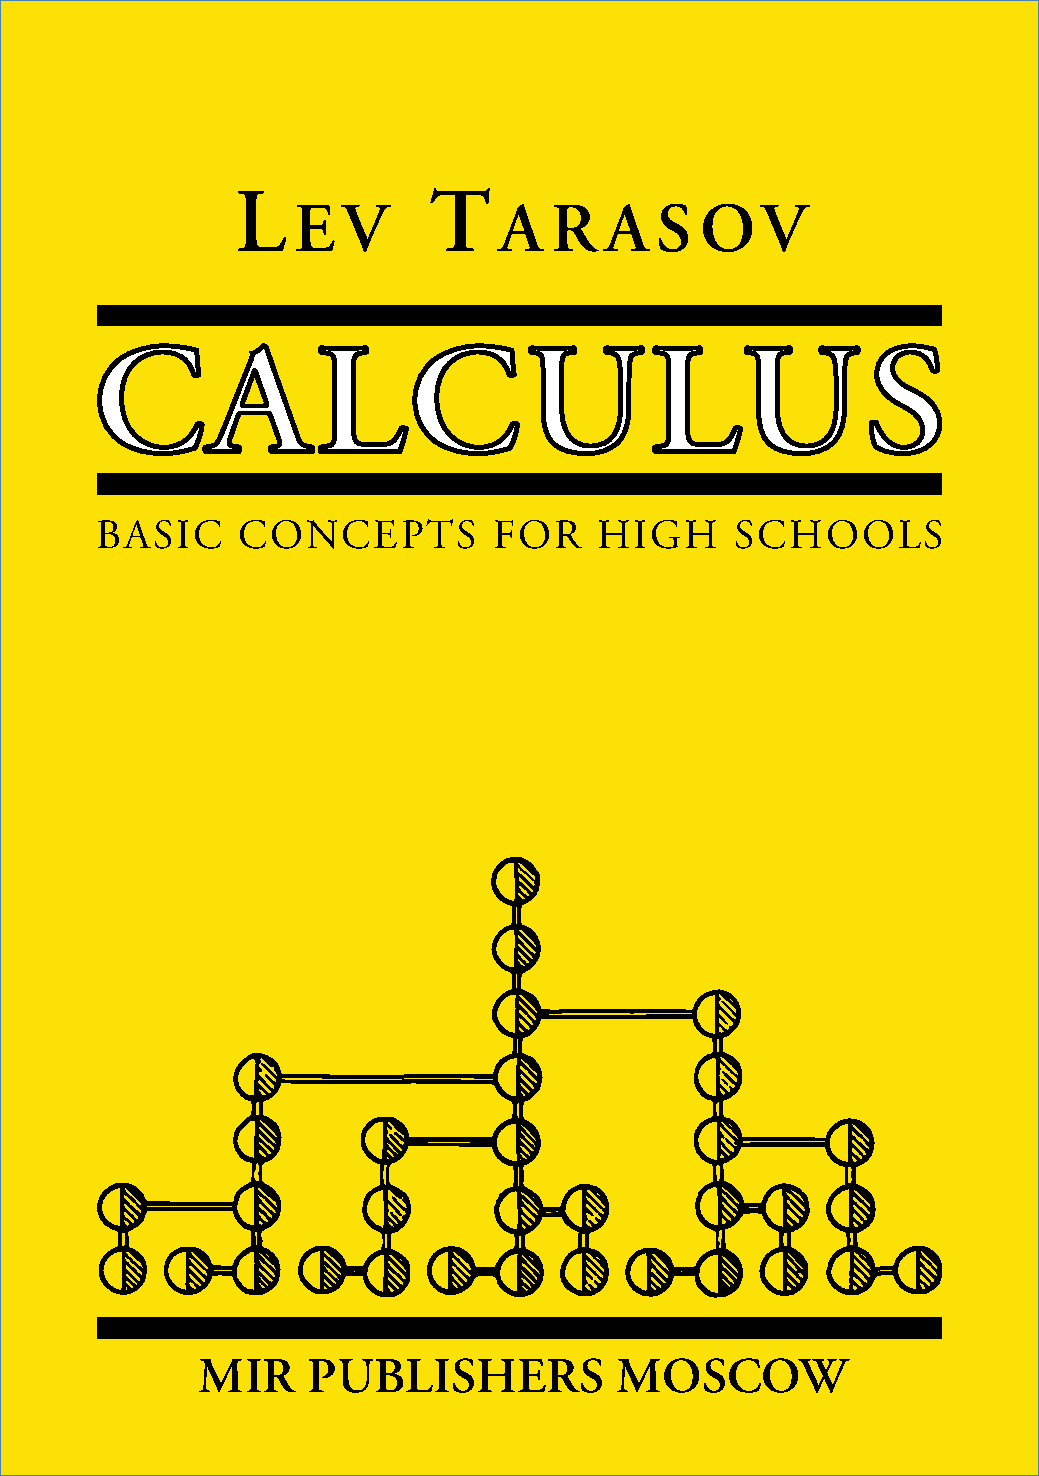
\includepdf{tarasov-calculus-fc.pdf}

\arrayrulecolor{gray} % <sets color of the \hline in tables
%\verbatimfontfamily{inconsolata}
%\maketitle
\thispagestyle{empty}

\frontmatter
%\thispagestyle{empty}
%11.B. TapaCOB
%OCHOBbl
%KBAHTOBO MEXAHK
%HSA9.TanbCTBO Bwcwafl WKOna MOCKBa
%\newpage
\thispagestyle{empty}
\vspace*{5cm}
\begin{center}
\begin{Huge}
%\hspace{1cm}
\textcolor{IndianRed}{\textsc{\fontsize{40}{45}\selectfont Lev Tarasov}}\\[1cm] 
%\noindent
%\hspace{1cm}
\textcolor{DodgerBlue}{\textsc{\fontsize{60}{65}\selectfont Calculus }}\\[1cm]
\end{Huge}
%\vspace{3cm}
%\begin{large}
%\fontsize{60}{65}\selectfont foo
%\end{large}
\vspace{7cm}
%\begin{huge}
\textsc{\fontsize{20}{25}\selectfont Mir Publishers Moscow}
%\end{huge}
\end{center}
\newpage
\thispagestyle{empty}

%\cleardoublepageb
\noindent
\begin{smaller}
Translated from the Russian by \emph{V. Kisin} and \emph{A. Zilberman}\\
First published 1988 \\
\noindent
Revised from the 1984 Russian edition \\[10pt]
\noindent
%\begin{tcolorbox}
This electronic version typeset using \XeLaTeX{} by \emph{Damitr Mazanov}.  \\ 
Released on the web by \textcolor{DodgerBlue}{\url{http://mirtitles.org}} in 2018.
%\end{tcolorbox}
\setcounter{tocdepth}{3}
\end{smaller}
\cleardoublepage
%\dominitoc
\tableofcontents

%\begin{savequote}[0.55\linewidth]

%\newline
%\qauthor{F. Engels}
%\end{savequote}

% !TEX root = calculus.tex

\chapter*{Preface}
\addcontentsline{toc}{chapter}{Preface}

\epigraph{Many objects are obscure to us not because our perceptions are poor, but simply because these objects are outside of the realm of our conceptions.}{Kosma Prutkov}

%{\parindent=0pt
\textcolor{IndianRed}{\textsc{Confession Of The Author}} My first acquaintance with calculus (or mathematical analysis) dates back to nearly a quarter of a century. This happened in the Moscow Engineering Physics Institute during splendid lectures given at that time by Professor D. A. Vasilkov. Even now I remember that feeling of delight and almost happiness. In the discussions with my classmates I rather heatedly insisted on a simile of higher mathematics to literature, which at that time was to me the most admired subject. Sure enough, these comparisons of mine lacked in objectivity. Nevertheless, my arguments were to a certain extent justified. The presence of an inner logic, coherence, dynamics, as well as the use of the most precise words to express a way of thinking, these were the characteristics of the prominent pieces of literature. They were present, in a different form of course, in higher mathematics as well. I remember that all of a sudden elementary mathematics which until that moment had seemed to me very dull and stagnant, turned to be brimming with life and inner motion governed by an impeccable logic.

Years have passed. The elapsed period of time has inevitably erased that highly emotional perception of calculus which has become a working tool for me. However, my memory keeps intact that unusual happy feeling which I experienced at the time of my initiation to this extraordinarily beautiful world of ideas which we call higher mathematics.

\textcolor{DodgerBlue}{\textsc{Confession Of The Reader}} Recently our professor of mathematics told us that we begin to study a new subject which he called calculus. He said that this subject is a foundation of higher mathematics and that it is going to be very difficult. We have already studied real numbers, the real line, infinite numerical sequences, and limits of sequences. The professor was indeed right saying that com.. prehension of the subject would present difficulties. I listen very carefully to his explanations and during the same day study the relevant pages of my textbook. I seem to understand everything, but at the same time have a feeling of a certain dissatisfaction. It is difficult for me to construct a consistent picture out of the pieces obtained in the classroom. It is equally difficult to remember exact wordings and definitions, for example, the definition of the limit of sequence. In other words, I fail to grasp something very important.
Perhaps, all things will become clearer in the future, but so far calculus has not become an open book for me. Moreover, I do not see any substantial difference between calculus and algebra. It seems that everything has become rather difficult to perceive and even more difficult to keep in my memory.

\textcolor{IndianRed}{\textsc{Comments Of The Author}} These two confessions provide an opportunity to get acquainted with the two interlocutors in this book. In fact, the whole book is presented as a relatively free-flowing dialogue between the AUTHOR and the READER. From one discussion to another the AUTHOR will lead the inquisitive and receptive READER to different notions, ideas, and theorems of calculus, emphasizing especially complicated or delicate aspects, stressing the inner logic of proofs, and attracting the reader's attention to special points. I hope that this form of presentation will help a reader of the book in learning new definitions such as those of \emph{derivative, antiderivative, definite integral, differential equation}, etc. I also expect that it will lead the reader to better understanding of such concepts as \emph{numerical sequence, limit of sequence, and function}. Briefly, these discussions are intended to assist pupils entering a novel world of calculus.And if in the long run the reader of the book gets a feeling of the intrinsic beauty and integrity of higher mathematics or even is appealed to it the author will consider his mission as successfully completed.	

Working on this book, the author consulted the existing manuals and textbooks such as \emph{Algebra and Elements of Analysis} edited by A. N. Kolmogorov, as well as the specialized textbook by N. Ya. Vilenkin and S. I. Shvartsburd \emph{Calculus}. Appreciable help was given to the author in the form of comments and recommendations by N. Ya. Vilenkin, B. M. Ivlev, A. M. Kisin, S. N. Krachkovsky, and N. Ch. Krutitskaya, who read the first version of the manuscript. I wish to express gratitude for their advice and interest in my work. I am especially grateful to A. N. Tarasova for her help in preparing the manuscript.
%}

\cleardoublepage
\mainmatter

% !TEX root = calculus.tex
\chapter{INFINITE NUMERICAL SEQUENCE}
\label{infinite-seq}
{\parindent=0pt
\athr Let us start our discussions of calculus by considering the definition of an \emph{infinite numerical sequence} or simply a \emph{sequence}.

We shall consider the following examples of sequences:
\begin{align}%
 1, \, 2, \, 4, \, 8, \, 16, \, 32, \, 64, \, 128, \, \ldots \label{series-01}\\
 5, \, 7, \, 9, \, 11, \, 13, \, 15, \, 17, \, 19, \, \ldots \label{series-02}\\
1, \, 4, \, 9, \, 16, \, 25, \, 36, \, 49, \, 64, \, \ldots \label{series-03}\\
1,\, \sqrt{2}, \, \sqrt{3}, \, 2, \, \sqrt{5}, \, \sqrt{6}, \, \sqrt{7}, \, 2 \sqrt{2}, \, \ldots \label{series-04}\\
\frac{1}{2}, \,\frac{2}{3}, \,\frac{3}{4}, \,\frac{4}{5}, \,\frac{5}{6}, \,\frac{6}{7}, \,\frac{7}{8}, \,\frac{8}{9}, \, \ldots \label{series-05}\\
2, \, 0, \, - 2, \, - 4, \, - 6, \, - 8, \, - 10, \, - 12, \, \ldots \label{series-06}\\
1, \frac{1}{2}, \,\frac{1}{3}, \,\frac{1}{4}, \,\frac{1}{5}, \,\frac{1}{6}, \,\frac{1}{7}, \,\frac{1}{8}, \, \ldots \label{series-07}\\
1, \frac{1}{2}, \, 3, \, \frac{1}{4}, \, 5, \,\frac{1}{6}, \, 7, \,\frac{1}{8}, \, \ldots \label{series-08}\\
1, \, -1, \, \frac{1}{3}, \, -\frac{1}{3}, \, \frac{1}{5}, \, -\frac{1}{5}, \, \frac{1}{7}, \, -\frac{1}{7}, \, \ldots \label{series-09}\\
1, \frac{2}{3}, \,\frac{1}{3}, \,\frac{1}{4}, \,\frac{1}{5}, \,\frac{6}{7}, \,\frac{1}{7}, \,\frac{8}{9}, \, \ldots \label{series-10}
\end{align}
Have a closer look at these examples. What do they have in common?

\rdr It is assumed that in each example there must be an infinite number of terms in a sequence. But in general, they are all different.

\athr In each example we have eight terms of a sequence. Could you write, say, the ninth term?

\rdr Sure, in the first example the ninth term must be 256, while in the second example it must be 21.

\athr Correct. It means that in all the examples there is a \emph{certain law}, which makes it possible to write down the ninth, tenth, and other terms of the sequences. Note, though, that if there is a \emph{finite number} of terms in a sequence, one may fail to discover the law which governs the infinite sequence.

\rdr Yes, but in our case these laws are easily recognizable. In example \eqref{series-01} we have the terms of an infinite geometric progression with common ratio 2. In example \eqref{series-02} we notice a sequence of odd numbers starting from 5. In example \eqref{series-03} we recognize a sequence of squares of natural numbers.

\athr Now let us look at the situation more rigorously. Let us enumerate all the terms of the sequence in sequential order, i.e. $1, \, 2, \, 3, \ldots, \,n, \ldots$  There is a certain law (a rule) by which each of these natural numbers is \emph{assigned} to a certain number (the corresponding term of the sequence). In example \eqref{series-01} this arrangement is as follows:
{\smaller \begin{center}
\begin{tabular}{cccccccccl}
\noalign{\global\arrayrulewidth=.5mm}
  \arrayrulecolor{DodgerBlue}
\hline
1 & 2 & 4 & 8 & 16 & 32 & \ldots & $2^{n-1}$ & \ldots & (terms of the sequence) \\
$\uparrow$ & $\uparrow$ & $\uparrow$ & $\uparrow$ & $\uparrow$ & $\uparrow$ &  & $\uparrow$ &  &   \\
1 & 2 & 3 & 4 & 5 & 6 & \ldots & $n$ & \ldots & (position numbers of the terms)\\
\hline
\end{tabular}
\end{center}}
In order to describe a sequence it is sufficient to indicate the term of the sequence corresponding to the number $n$, i.e. to write down the term of the sequence occupying the nth position. Thus, we can formulate the following definition of a sequence. 
\begin{mytheo}{Definition}
We say that there is an infinite numerical sequence if every
natural number (position numbers is unambiguously placed in correspondence with a definite number (term of the sequence) by a specific rule.
\end{mytheo}
This relationship may be presented in the following general form:
{\smaller \begin{center}
\begin{tabular}{cccccccc}
\noalign{\global\arrayrulewidth=.5mm}
  \arrayrulecolor{DodgerBlue}
\hline
$y_{1}$ & $y_{2}$ & $y_{3}$ & $y_{4}$ & $y_{5}$ & \ldots & $y_{n}$ & \ldots \\
$\uparrow$ & $\uparrow$ & $\uparrow$ & $\uparrow$ & $\uparrow$ &    & $\uparrow$  &   \\
1 & 2 & 3 & 4 & 5 & \ldots & $n$ & \ldots  \\ 
 \hline
\end{tabular}
\end{center}}
'The number $y_{n}$  is the $n$th term of the sequence, and the whole sequence is sometimes denoted by a symbol ($y_{n}$).

\rdr We have been given a somewhat different definition of a sequence: a sequence is a function defined on a set of natural numbers (integers).

\athr Well, actually the two definitions are equivalent. However, I am not inclined to use the term ``function'' too early. First, because the discussion of a function will come later. Second, you will normally deal with somewhat
different functions, namely those defined not on a set of integers but on the real line or within its segment. Anyway, the above definition of a sequence is quite correct.

Getting back to our examples of sequences, let us look in each case for an \emph{analytical expression (formula)} for the $n$th term. Go ahead.

\rdr Oh, this is not difficult. In example \eqref{series-01} it is $y_{n}=2^{n}$. In \eqref{series-02} it is  $y_{n}=2n+3$. In \eqref{series-03} it is  $y_{n}= n^{2}$. In \eqref{series-04} it is  $y_{n}= \sqrt{n}$. In \eqref{series-05} it is  $y_{n}=1 - \dfrac{1}{n+1}= \dfrac{n}{n+1}$. In \eqref{series-06} it is  $y_{n}=4- 2n$. In \eqref{series-07} it is  $y_{n}= \dfrac{1}{n}$.

In the remaining three examples I just do not know. 

\athr Let us look at example \eqref{series-08}. One can easily see that if $n$ is an even integer, then $y_{n}=\dfrac{1}{n}$, but if $n$ is odd, then $y_{n} = n$, It means that 
\begin{equation*}%
y_{n}= 
\begin{cases}
\dfrac{1}{n} \,\, \text{if} \,\, n=2k \\
n  \,\, \text{if} \,\, n= 2k-1
\end{cases}
\end{equation*}
\rdr Can I, in this particular case, find a single analytical expression for $y_{n}$?

\athr Yes, you can. Though I think you needn't. Let us present $y_{n}$ in a different form:
\begin{equation*}%
y_{n} = a_{n} n + b_{n} \frac{1}{n}
\end{equation*}
and demand that the coefficient $a_{n}$ be equal to unity if $n$ is odd, and to zero if $n$ is even; the coefficient $b_{n}$ should behave in quite an opposite manner. In this particular case these coefficients can be determined as follows:
\begin{equation*}%
%\begin{split}
a_{n}  = \frac{1}{2} \left[1 - (-1)^{n} \right], \quad b_{n}  =  \frac{1}{2} \left[1 + (-1)^{n} \right] 
%\end{split}
\end{equation*}
Consequently 
\begin{equation*}%
y_{n}  = \frac{n}{2} \left[1 - (-1)^{n} \right]+  \frac{1}{2n} \left[1 + (-1)^{n} \right] 
\end{equation*}
Do in the same manner in the other two examples. 

\rdr For sequence  \eqref{series-09} I can write
\begin{equation*}%
y_{n}  = \frac{1}{2n} \left[1 - (-1)^{n} \right]+  \frac{1}{2(n-1)} \left[1 + (-1)^{n} \right] 
\end{equation*}
and for sequence \eqref{series-10}
\begin{equation*}%
y_{n}  = \frac{1}{2n} \left[1 - (-1)^{n} \right]+  \frac{n}{2(n+1)} \left[1 + (-1)^{n} \right] 
\end{equation*}

\athr It is important to note that an analytical expression for the nth term of a given sequence is not necessarily a unique method of defining a sequence. A sequence can be defined, for example, by \emph{recursion} (or the \emph{recurrence method}) (Latin word \emph{recurrere} means to run back). In this case, in order to define a sequence one should describe the first term (or the first several terms) of the sequence and a recurrence (or a recursion) relation, which is an expression for the $n$th term of the sequence via the preceding one (or several preceding terms).

Using the recurrence method, let us present sequence \eqref{series-01}, as follows
\begin{equation*}%
y_{1	} = 1, \quad y_{n}  = 2  y_{n - 1}  
\end{equation*}

\rdr It's clear. Sequence \eqref{series-02} can be apparently represented by formulas 
\begin{equation*}%
y_{1	} = 5, \quad y_{n}  = y_{n - 1}  + 2
\end{equation*}

\athr That's right. Using recursion, let us try to determine one interesting sequence
\begin{equation*}%
y_{1	} = 1, \quad y_{2} = 1, \quad y_{n}  =   y_{n - 2} +   y_{n - 1}  
\end{equation*}
\begin{equation}%
1, \, 1, \, 2, \, 3, \, 5, \, 8, \, 13, \, 21, \ldots
\label{fibonacci}
%eq-11
\end{equation}
This sequence is known as the \emph{Fibonacci sequence} (or \emph{numbers}).

\rdr I understand, I have heard something about. the problem of Fibonacci rabbits.

\athr Yes, it was this problem, formulated by Fibonacci, the 13th century Italian mathematician, that gave the name to this sequence \eqref{fibonacci}. The problem reads as follows. A man places a pair of newly born rabbits into a warren and wants to know how many rabbits he would have over a certain period of time. A pair of rabbits will start producing offspring two months after they were born and every following month one new pair of rabbits will appear. At the beginning (during the first month) the man will have in his warren only one pair of rabbits ($y_{1} = 1$); during the second month he will have the same pair of rabbits ($y_{2} = 1$); during the third month the offspring will appear, and therefore the number of the pairs of rabbits in the warren will grow to two ($y_{3} = 3$); during the fourth month there will be one more reproduction of the first pair ($y_{4} = 3$); during the fifth month there will be offspring both from the first and second couples of rabbits ($y_{5} = 5$), etc. An increase of the number of pairs in the warren from month to month is plotted in \fig{fig-01}. One can see that the numbers of pairs of rabbits counted at the end of each month form sequence \eqref{fibonacci}, i.e. the Fibonacci, sequence.

\begin{figure}[!h]
\centering
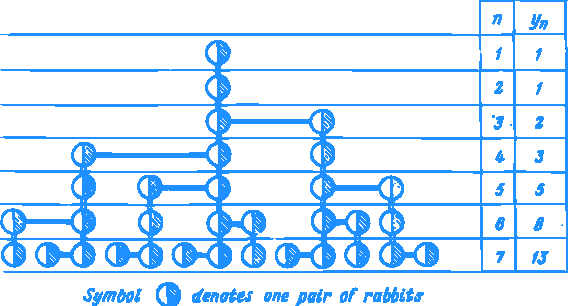
\includegraphics[width=0.9\textwidth]{figures/fig-01.pdf}
\caption{Visualising Fibonacci rabbits.}
\label{fig-01}
\end{figure}

\rdr But in reality the rabbits do not multiply in accordance with such an idealized pattern. Furthermore, as time goes on, the first pairs of rabbits should obviously stop proliferating.

\athr The Fibonacci sequence is interesting not because it describes a simplified growth pattern of rabbits' population. It so happens that this sequence appears, as if by magic, in quite unexpected situations. For example, the Fibonacci numbers are used to process information by computers and to optimize programming for computers. However, this is a digression from our main topic.

Getting back to the ways of describing sequences, I would like to point out that the \emph{very method chosen to describe a sequence is not of principal importance}. One sequence may be described, for the sake of convenience, by a formula for the $n$th term, and another (as, for example, the Fibonacci sequence), by the recurrence method. What is important, however, is the method used to describe the \emph{law of correspondence}, i.e. the law by which any natural number is placed in correspondence with a certain term of the sequence. In a number of cases such a law can be formulated only by words. The examples of such cases are shown below:
\begin{align}%
2, \, 3, \, 5, \, 7, \, 11, \, 13, \, 17, \, 19, \, 23, \ldots \label{series-12}\\
3,  \, 3.1, \,  3.14, \,  3.141, \,  3.1415, \,  3.14159, \ldots \label{series-13}
\end{align}

In both cases we cannot indicate either the formula for the- nth term or the recurrence relation. Nevertheless, you can without great difficulties identify specific laws of correspondence and put them in words.

\rdr Wait a minute. Sequence \eqref{series-12} is a sequence of \emph{prime numbers} arranged in an increasing order, while \eqref{series-13} is, apparently, a sequence composed of decimal approximations, with deficit, for $\pi$.

\athr You are absolutely right.

\rdr It may seem that a numerical sequence differs from a random set of numbers by a presence of an intrinsic \emph{degree of order} that is reflected either by the formula for tho $n$th term or by the recurrence relation. However, the last two examples show that such a degree of order needn't. be present.
%\begin{figure}[!h]
%\centering
%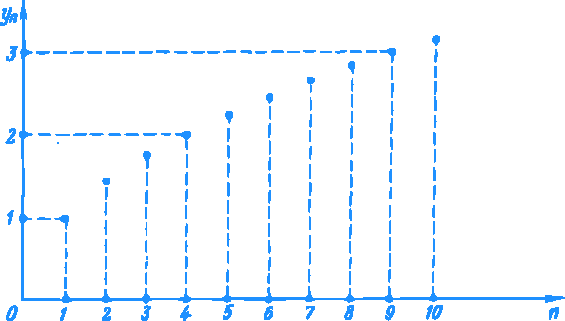
\includegraphics[width=0.9\textwidth]{figures/fig-02.pdf}
%\caption{Graph of the series \eqref{series-04}.}
%\label{fig-02}
%\end{figure}

\begin{figure}[!h]
\centering
\begin{tikzpicture}[line cap=round,line join=round,>=triangle 45,x=1.0cm,y=1.0cm]
%\filldraw[->,color=black] (-0.8900469095523698,0.) -- (11.877941351923667,0.);
\foreach \x in {,1,2,3,4,5,6,7,8,9,10}
\filldraw[shift={(\x,0)},color=black] (0pt,2pt) -- (0pt,-2pt) node[below] {\footnotesize $\x$};
%\filldraw[->,color=black] (0.,-0.9081072000876554) -- (0.,6.37592544744293);
\foreach \y in {0,1,2,3}
\filldraw[shift={(0,\y)},color=black] (2pt,0pt) -- (-2pt,0pt) node[left] {\footnotesize $\y$};
%\filldraw[color=black] (0pt,-10pt) node[below] {\footnotesize $0$};
\clip(-0.8900469095523698,-0.9081072000876554) rectangle (11.5,4);
\draw[color=black] (0,3.5) node[left] { $y_{n}$};
\draw[color=black] (11,0) node[below] { $n$};
\filldraw [line width=0.5pt,dash pattern=on 3pt off 3pt,color=DarkGray] (1.,1.)-- (1.,0.);
\filldraw [line width=0.5pt,dash pattern=on 3pt off 3pt,color=DarkGray] (2.,1.4142135623730951)-- (2.,0.);
\filldraw [line width=0.5pt,dash pattern=on 3pt off 3pt,color=DarkGray] (3.,1.7320508075688772)-- (3.,0.);
\filldraw [line width=0.5pt,dash pattern=on 3pt off 3pt,color=DarkGray] (4.,2.)-- (4.,0.);
\filldraw [line width=0.5pt,dash pattern=on 3pt off 3pt,color=DarkGray] (5.,2.23606797749979)-- (5.,0.);
\filldraw [line width=0.5pt,dash pattern=on 3pt off 3pt,color=DarkGray] (6.,2.449489742783178)-- (6.,0.);
\filldraw [line width=0.5pt,dash pattern=on 3pt off 3pt,color=DarkGray] (7.,2.6457513110645907)-- (7.,0.);
\filldraw [line width=0.5pt,dash pattern=on 3pt off 3pt,color=DarkGray] (8.,2.8284271247461903)-- (8.,0.);
\filldraw [line width=0.5pt,dash pattern=on 3pt off 3pt,color=DarkGray] (1.,1.)-- (0.,1.);
\filldraw [line width=0.5pt,dash pattern=on 3pt off 3pt,color=DarkGray] (4.,2.)-- (0.,2.);
\filldraw [line width=0.5pt,dash pattern=on 3pt off 3pt,color=DarkGray] (9.,3.)-- (9.,0.);
\filldraw [line width=0.5pt,dash pattern=on 3pt off 3pt,color=DarkGray] (9.,3.)-- (0.,3.);
\filldraw [line width=0.5pt,dash pattern=on 3pt off 3pt,color=DarkGray] (10.,3.1622776601683795)-- (10.,0.);
\filldraw [->,line width=1.2pt,color=DarkGray] (0.,0.) -- (0.,3.75);
\filldraw [->,line width=1.2pt,color=DarkGray] (0.,0.) -- (11,0);
\begin{scriptsize}
\filldraw [IndianRed] (1.,1.) circle (2.5pt);
\filldraw [IndianRed] (2.,1.4142135623730951) circle (2.5pt);
\filldraw [IndianRed] (3.,1.7320508075688772) circle (2.5pt);
\filldraw [IndianRed] (4.,2.) circle (2.5pt);
\filldraw [IndianRed] (5.,2.23606797749979) circle (2.5pt);
\filldraw [IndianRed] (6.,2.449489742783178) circle (2.5pt);
\filldraw [IndianRed] (7.,2.6457513110645907) circle (2.5pt);
\filldraw [IndianRed] (8.,2.8284271247461903) circle (2.5pt);
\filldraw [DodgerBlue] (1.,0.) circle (2.5pt);
\filldraw [DodgerBlue] (2.,0.) circle (2.5pt);
\filldraw [DodgerBlue] (3.,0.) circle (2.5pt);
\filldraw [DodgerBlue] (4.,0.) circle (2.5pt);
\filldraw [DodgerBlue] (5.,0.) circle (2.5pt);
\filldraw [DodgerBlue] (6.,0.) circle (2.5pt);
\filldraw [DodgerBlue] (7.,0.) circle (2.5pt);
\filldraw [DodgerBlue] (8.,0.) circle (2.5pt);
\filldraw [DodgerBlue] (0.,1.) circle (2.5pt);
\filldraw [DodgerBlue] (0.,2.) circle (2.5pt);
\filldraw [IndianRed] (9.,3.) circle (2.5pt);
\filldraw [IndianRed] (10.,3.1622776601683795) circle (2.5pt);
\filldraw [DodgerBlue] (9.,0.) circle (2.5pt);
\filldraw [DodgerBlue] (0.,3.) circle (2.5pt);
\filldraw [DodgerBlue] (10.,0.) circle (2.5pt);
\end{scriptsize}
\end{tikzpicture}
%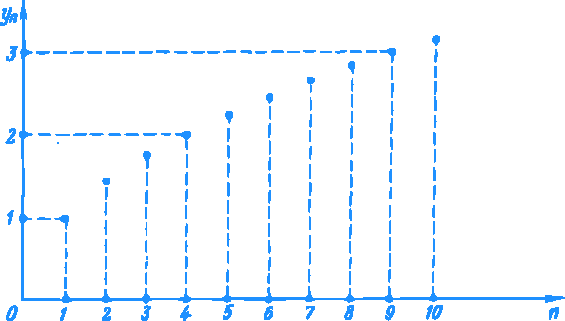
\includegraphics[width=0.9\textwidth]{figures/fig-02.pdf}
\caption{Graph of the series \eqref{series-04}.}
\label{fig-02}
\end{figure}

\athr Actually, a degree of order determined by a formula (an analytical expression) is not mandatory. It is important, however, to have a law (a rule, a characteristic) of correspondence, which enables one to relate any natural number to a certain term of a sequence. In examples \eqref{series-12} and \eqref{series-13} such laws of correspondence are obvious. Therefore,
\eqref{series-12} and \eqref{series-13} are not inferior (and not superior) to sequences \eqref{series-01}-\eqref{fibonacci} which permit an analytical description.
 \begin{figure}[!h]
\centering
\begin{tikzpicture}[line cap=round,line join=round,>=triangle 45,x=1.0cm,y=3.5cm]
\foreach \x in {,1,2,3,4,5,6,7,8,9,10}
\draw[shift={(\x,0)},color=black] (0pt,2pt) -- (0pt,-2pt) node[below] {\footnotesize $\x$};
\foreach \y in {,0,1}
\draw[shift={(0,\y)},color=black] (2pt,0pt) -- (-2pt,0pt) node[left] {\footnotesize $\y$};
%\draw[color=black] (0pt,-10pt) node[right] {\footnotesize $0$};
\draw[color=black] (0,1.2) node[left] { $y_{n}$};
\draw[color=black] (11,0) node[below] { $n$};
\clip(-0.7,-0.10) rectangle (11.5,1.3);
\draw [line width=1pt,color=IndianRed,dash pattern=on 3pt off 3pt,domain=0:11.5] plot(\x,{(--1.-0.*\x)/1.});
\draw [->,line width=1.2pt,color=DarkGray] (0.,0.) -- (0.,1.3);
\draw [->,line width=1.2pt,color=DarkGray] (0.,0.) -- (11.,0.);
\draw [line width=.75pt,dash pattern=on 3pt off 3pt,color=DarkGray] (1.,0.5)-- (1.,0.);
\draw [line width=.75pt,dash pattern=on 3pt off 3pt,color=DarkGray] (2.,0.6666666666666666)-- (2.,0.);
\draw [line width=.75pt,dash pattern=on 3pt off 3pt,color=DarkGray] (3.,0.75)-- (3.,0.);
\draw [line width=.75pt,dash pattern=on 3pt off 3pt,color=DarkGray] (4.,0.8)-- (4.,0.);
\draw [line width=.75pt,dash pattern=on 3pt off 3pt,color=DarkGray] (5.,0.8333333333333334)-- (5.,0.);
\draw [line width=.75pt,dash pattern=on 3pt off 3pt,color=DarkGray] (6.,0.8571428571428571)-- (6.,0.);
\draw [line width=.75pt,dash pattern=on 3pt off 3pt,color=DarkGray] (7.,0.875)-- (7.,0.);
\draw [line width=.75pt,dash pattern=on 3pt off 3pt,color=DarkGray] (8.,0.8888888888888888)-- (8.,0.);
\draw [line width=.75pt,dash pattern=on 3pt off 3pt,color=DarkGray] (9.,0.9)-- (9.,0.);
\draw [line width=.75pt,dash pattern=on 3pt off 3pt,color=DarkGray] (10.,0.9090909090909091)-- (10.,0.);
\begin{scriptsize}
\filldraw [DodgerBlue] (1.,0.) circle (2.5pt);
\filldraw [DodgerBlue] (2.,0.) circle (2.5pt);
\filldraw [DodgerBlue] (3.,0.) circle (2.5pt);
\filldraw [DodgerBlue] (4.,0.) circle (2.5pt);
\filldraw [DodgerBlue] (5.,0.) circle (2.5pt);
\filldraw [DodgerBlue] (6.,0.) circle (2.5pt);
\filldraw [DodgerBlue] (7.,0.) circle (2.5pt);
\filldraw [DodgerBlue] (8.,0.) circle (2.5pt);
\filldraw [DodgerBlue] (0.,1.) circle (2.5pt);
\filldraw [DodgerBlue] (9.,0.) circle (2.5pt);
\filldraw [DodgerBlue] (0.,3.) circle (2.5pt);
\filldraw [DodgerBlue] (10.,0.) circle (2.5pt);
\filldraw [IndianRed] (1.,0.5) circle (2.5pt);
\filldraw [IndianRed] (2.,0.6666666666666666) circle (2.5pt);
\filldraw [IndianRed] (3.,0.75) circle (2.5pt);
\filldraw [IndianRed] (4.,0.8) circle (2.5pt);
\filldraw [IndianRed] (5.,0.8333333333333334) circle (2.5pt);
\filldraw [IndianRed] (6.,0.8571428571428571) circle (2.5pt);
\filldraw [IndianRed] (7.,0.875) circle (2.5pt);
\filldraw [IndianRed] (8.,0.8888888888888888) circle (2.5pt);
\filldraw [IndianRed] (9.,0.9) circle (2.5pt);
\filldraw [IndianRed] (10.,0.9090909090909091) circle (2.5pt);
\end{scriptsize}
\end{tikzpicture}
%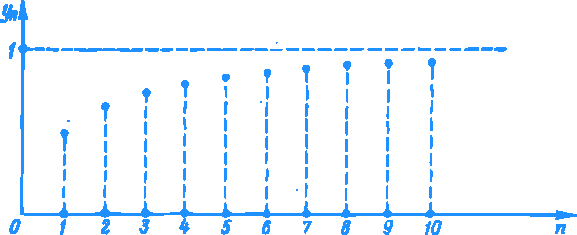
\includegraphics[width=0.9\textwidth]{figures/fig-03.pdf}
\caption{Image of the series \eqref{series-05}.}
\label{fig-03}
\end{figure}
 Later we shall talk about the \emph{geometric image} (or \emph{map}) of a numerical sequence. Let us take two coordinate axes, $x$ and $y$. We shall mark on the first axis integers $1, \, 2, \, 3, \ldots, n, \ldots$ and on the second axis, the corresponding terms of a sequence, i.e. the numbers $y_{1}, \, y_{2}, \, y_{3}, \ldots y_{n}, \ldots$. Then the sequence can be represented by a set of points $M (n, y_{n})$ on the coordinate plane. For example \fig{fig-02} images sequence \eqref{series-04}, \fig{fig-03} images sequence \eqref{series-05}, \fig{fig-04} images sequence \eqref{series-09}, and \fig{fig-05} images sequence \eqref{series-10}.
\begin{figure}[!h]
\centering
\begin{tikzpicture}[line cap=round,line join=round,>=triangle 45,x=1.0cm,y=3.5cm]
\foreach \x in {1,2,3,4,5,6,7,9}
\draw[shift={(\x,0)},color=black] (0pt,2pt) -- (0pt,-2pt) node[below] {\footnotesize $\x$};
\foreach \y in {-1,0,1}
\draw[shift={(0,\y)},color=black] (2pt,0pt) -- (-2pt,0pt) node[left] {\footnotesize $\y$};
\clip(-1.4,-1.1) rectangle (11.4,1.3);
\draw (-0.641960402073037,1.1784020472890375) node[anchor=north west] {$y_{n}$};
\draw (11,0) node[anchor=north west] {$n$};
\draw (10,-0.015) node[anchor=north west] {\footnotesize $10$};
\draw (8,-0.015) node[anchor=north west] {\footnotesize $8$};
\draw [->,line width=1.2pt,color=DarkGray] (0.,-1.0) -- (0.,1.2);
\draw [->,line width=1.2pt,color=DarkGray] (0.,0.) -- (11.2,0.);
\draw [line width=.75pt,dash pattern=on 3pt off 3pt,color=DarkGray] (0.,1.)-- (1.,1.);
\draw [line width=.75pt,dash pattern=on 3pt off 3pt,color=DarkGray] (1.,1.)-- (1.,0.);
\draw [line width=.75pt,dash pattern=on 3pt off 3pt,color=DarkGray] (0.,-1.)-- (2.,-1.);
\draw [line width=.75pt,dash pattern=on 3pt off 3pt,color=DarkGray] (2.,-1.)-- (2.,0.);
\draw [line width=.75pt,dash pattern=on 3pt off 3pt,color=DarkGray] (0.,0.3333333333333333)-- (3.,0.3333333333333333);
\draw [line width=.75pt,dash pattern=on 3pt off 3pt,color=DarkGray] (3.,0.3333333333333333)-- (3.,0.);
\draw [line width=.75pt,dash pattern=on 3pt off 3pt,color=DarkGray] (4.,0.)-- (4.,-0.3333333333333333);
\draw [line width=.75pt,dash pattern=on 3pt off 3pt,color=DarkGray] (4.,-0.3333333333333333)-- (0.,-0.3333333333333333);
\draw [line width=.75pt,dash pattern=on 3pt off 3pt,color=DarkGray] (0.,0.2)-- (5.,0.2);
\draw [line width=.75pt,dash pattern=on 3pt off 3pt,color=DarkGray] (5.,0.2)-- (5.,0.);
\draw [line width=.75pt,dash pattern=on 3pt off 3pt,color=DarkGray] (6.,0.)-- (6.,-0.2);
\draw [line width=.75pt,dash pattern=on 3pt off 3pt,color=DarkGray] (0.,-0.2)-- (6.,-0.2);
\draw [line width=.75pt,dash pattern=on 3pt off 3pt,color=DarkGray] (7.,0.14285714285714285)-- (7.,0.);
\draw [line width=.75pt,dash pattern=on 3pt off 3pt,color=DarkGray] (8.,-0.14285714285714285)-- (8.,0.);
\draw [line width=.75pt,dash pattern=on 3pt off 3pt,color=DarkGray] (9.,0.125)-- (9.,0.);
\draw [line width=.75pt,dash pattern=on 3pt off 3pt,color=DarkGray] (10.,-0.125)-- (10.,0.);
\begin{scriptsize}
\filldraw [IndianRed] (1.,1.) circle (2.5pt);
\filldraw [IndianRed] (2.,-1.) circle (2.5pt);
\filldraw [IndianRed] (3.,0.3333333333333333) circle (2.5pt);
\filldraw [IndianRed] (4.,-0.3333333333333333) circle (2.5pt);
\filldraw [IndianRed] (5.,0.2) circle (2.5pt);
\filldraw [IndianRed] (6.,-0.2) circle (2.5pt);
\filldraw [IndianRed] (7.,0.14285714285714285) circle (2.5pt);
\filldraw [IndianRed] (8.,-0.14285714285714285) circle (2.5pt);
\filldraw [DodgerBlue] (1.,0.) circle (2.5pt);
\filldraw [DodgerBlue] (2.,0.) circle (2.5pt);
\filldraw [DodgerBlue] (3.,0.) circle (2.5pt);
\filldraw [DodgerBlue] (4.,0.) circle (2.5pt);
\filldraw [DodgerBlue] (5.,0.) circle (2.5pt);
\filldraw [DodgerBlue] (6.,0.) circle (2.5pt);
\filldraw [DodgerBlue] (7.,0.) circle (2.5pt);
\filldraw [DodgerBlue] (8.,0.) circle (2.5pt);
\filldraw [DodgerBlue] (9.,0.) circle (2.5pt);
\filldraw [DodgerBlue] (10.,0.) circle (2.5pt);
\filldraw [DodgerBlue] (0.,0.3333333333333333) circle (2.5pt);
\filldraw [DodgerBlue] (0.,-0.3333333333333333) circle (2.5pt);
\filldraw [DodgerBlue] (0.,0.2) circle (2.5pt);
\filldraw [DodgerBlue] (0.,-0.2) circle (2.5pt);
\filldraw [DodgerBlue] (0.,1.) circle (2.5pt);
\filldraw [DodgerBlue] (0.,0.) circle (2.5pt);
\filldraw [DodgerBlue] (0.,-1.) circle (2.5pt);
\filldraw [IndianRed] (9.,0.125) circle (2.5pt);
\filldraw [IndianRed] (10.,-0.125) circle (2.5pt);
\end{scriptsize}
\end{tikzpicture}
%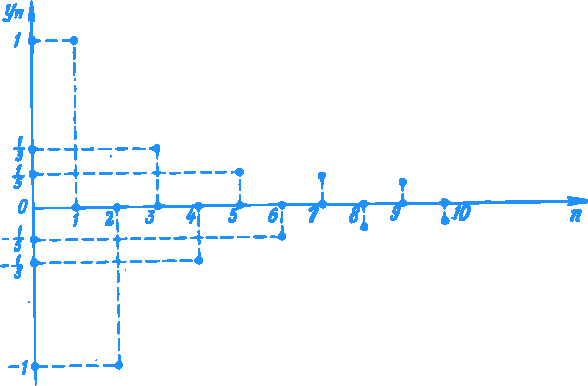
\includegraphics[width=0.9\textwidth,angle=-1]{figures/fig-04.pdf}
\caption{Series in equation \eqref{series-09} visualised.}
\label{fig-04}

\end{figure}
\begin{figure}[!h]
\centering
\begin{tikzpicture}[line cap=round,line join=round,>=triangle 45,x=1.0cm,y=3.5cm]
\foreach \x in {1,2,3,4,5,6,7,8,9,10}
\draw[shift={(\x,0)},color=black] (0pt,2pt) -- (0pt,-2pt) node[below] {\footnotesize $\x$};
\foreach \y in {0,1}
\draw[shift={(0,\y)},color=black] (2pt,0pt) -- (-2pt,0pt) node[left] {\footnotesize $\y$};
\draw[shift={(0,0.33)},color=black]  (2pt,0pt) -- (-2pt,0pt) node[left] {\footnotesize $\dfrac{1}{3}$};
\draw[shift={(0,0.66)},color=black]  (2pt,0pt) -- (-2pt,0pt) node[left] {\footnotesize $\dfrac{2}{3}$};
\clip(-0.9,-0.12) rectangle (11,1.3);
\draw (-0.6,1.2) node[anchor=north west] {$y_{n}$};
\draw (10.457277999784147,-0.03) node[anchor=north west] {$n$};
\draw [->,line width=1.2pt,color=DarkGray] (0.,0.) -- (0.,1.25);
\draw [->,line width=1.2pt,color=DarkGray] (0.,0.) -- (11.,0.);
\draw [line width=.75pt,dash pattern=on 3pt off 3pt,color=DarkGray] (0.,1.)-- (1.,1.);
\draw [line width=.75pt,dash pattern=on 3pt off 3pt,color=DarkGray] (1.,1.)-- (1.,0.);
\draw [line width=1pt,dash pattern=on 3pt off 3pt,color=IndianRed,domain=0:11] plot(\x,{(--1.-0.*\x)/1.});
\draw [line width=.75pt,dash pattern=on 3pt off 3pt,color=DarkGray] (2.,0.6666666666666666)-- (2.,0.);
\draw [line width=.75pt,dash pattern=on 3pt off 3pt,color=DarkGray] (2.,0.6666666666666666)-- (0.,0.6666666666666666);
\draw [line width=.75pt,dash pattern=on 3pt off 3pt,color=DarkGray] (3.,0.3333333333333333)-- (0.,0.3333333333333333);
\draw [line width=.75pt,dash pattern=on 3pt off 3pt,color=DarkGray] (3.,0.3333333333333333)-- (3.,0.);
\draw [line width=.75pt,dash pattern=on 3pt off 3pt,color=DarkGray] (4.,0.75)-- (4.,0.);
\draw [line width=.75pt,dash pattern=on 3pt off 3pt,color=DarkGray] (5.,0.2)-- (5.,0.);
\draw [line width=.75pt,dash pattern=on 3pt off 3pt,color=DarkGray] (6.,0.8571428571428571)-- (6.,0.);
\draw [line width=.75pt,dash pattern=on 3pt off 3pt,color=DarkGray] (7.,0.14285714285714285)-- (7.,0.);
\draw [line width=.75pt,dash pattern=on 3pt off 3pt,color=DarkGray] (8.,0.8888888888888888)-- (8.,0.);
\draw [line width=.75pt,dash pattern=on 3pt off 3pt,color=DarkGray] (9.,0.1111111111111111)-- (9.,0.);
\draw [line width=.75pt,dash pattern=on 3pt off 3pt,color=DarkGray] (10.,0.9)-- (10.,0.);
\begin{scriptsize}
\filldraw [IndianRed] (1.,1.) circle (2.5pt);
\filldraw [DodgerBlue] (1.,0.) circle (2.5pt);
\filldraw [DodgerBlue] (2.,0.) circle (2.5pt);
\filldraw [DodgerBlue] (3.,0.) circle (2.5pt);
\filldraw [DodgerBlue] (4.,0.) circle (2.5pt);
\filldraw [DodgerBlue] (5.,0.) circle (2.5pt);
\filldraw [DodgerBlue] (6.,0.) circle (2.5pt);
\filldraw [DodgerBlue] (7.,0.) circle (2.5pt);
\filldraw [DodgerBlue] (8.,0.) circle (2.5pt);
\filldraw [DodgerBlue] (9.,0.) circle (2.5pt);
\filldraw [DodgerBlue] (10.,0.) circle (2.5pt);
\filldraw [DodgerBlue] (0.,1.) circle (2.5pt);
\filldraw [IndianRed] (2.,0.6666666666666666) circle (2.5pt);
\filldraw [IndianRed] (3.,0.3333333333333333) circle (2.5pt);
\filldraw [IndianRed] (4.,0.75) circle (2.5pt);
\filldraw [DodgerBlue] (0.,0.6666666666666666) circle (2.5pt);
\filldraw [DodgerBlue] (0.,0.3333333333333333) circle (2.5pt);
\filldraw [IndianRed] (5.,0.2) circle (2.5pt);
\filldraw [IndianRed] (6.,0.8571428571428571) circle (2.5pt);
\filldraw [IndianRed] (7.,0.14285714285714285) circle (2.5pt);
\filldraw [IndianRed] (8.,0.8888888888888888) circle (2.5pt);
\filldraw [IndianRed] (9.,0.1111111111111111) circle (2.5pt);
\filldraw [IndianRed] (10.,0.9) circle (2.5pt);
\end{scriptsize}
\end{tikzpicture}
%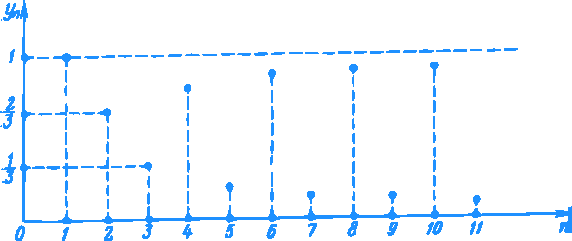
\includegraphics[width=0.9\textwidth,angle=-1]{figures/fig-05.pdf}
\caption{Series in equation \eqref{series-10} visualised.}
\label{fig-05}
\end{figure}

As a matter of fact, there are other types of geometry images of a numerical sequence. Let us retain, for example only one coordinate $y$-axis and plot on it points  $y_{1}, \, y_{2}, \, y_{3}, \ldots y_{n}, \ldots$ which map the terms of a sequence. In \fig{fig-06} this method of mapping is illustrated for the sequences that have been shown in \fig{fig-02}-\fig{fig-05}. One has to admit that the latter method is less descriptive in comparison with the former method.
\begin{figure}[!h]
\centering
\begin{tikzpicture}[baseline=1cm,line cap=round,line join=round,>=triangle 45,x=2.5cm,y=2.0cm]
\foreach \x in {0,1,2,3,4}
\draw[shift={(\x,0)},color=black] (0pt,2pt) -- (0pt,-2pt) node[below] {\footnotesize $\x$};
\clip(-0.3,-0.3) rectangle (5.,0.52);
\draw (4.212511655558804,0.008475512540077454) node[anchor=north west] {$y$};
\draw [->,line width=1.2pt,color=DarkGray] (0.,0.) -- (4.6,0.);
\draw (1.9,0.35) node[anchor=north west] {$y_{4}$};
\draw (2.88,0.35) node[anchor=north west] {$y_{9}$};
\draw (1.6,0.35) node[anchor=north west] {$y_{3}$};
\draw (1.3171801125876044,0.35) node[anchor=north west] {$y_{2}$};
\draw (0.9,0.35) node[anchor=north west] {$y_{1}$};
\draw (-0.1,0.5) node[anchor=north west,color=IndianRed] {\textit{Sequence} (4)};
\begin{scriptsize}
\filldraw [DodgerBlue] (11.,0.) circle (2.5pt);
\filldraw [DodgerBlue] (1.,0.) circle (2.5pt);
\filldraw [DodgerBlue] (2.,0.) circle (2.5pt);
\filldraw [DodgerBlue] (3.,0.) circle (2.5pt);
\filldraw [DodgerBlue] (4.,0.) circle (2.5pt);
\filldraw [DodgerBlue] (0.,0.) circle (2.5pt);
\filldraw [DodgerBlue] (1.,0.) circle (2.5pt);
\filldraw [DodgerBlue] (1.41,0.) circle (2.5pt);
\filldraw [DodgerBlue] (1.73,0.) circle (2.5pt);
\filldraw [DodgerBlue] (2.,0.) circle (2.5pt);
\filldraw [DodgerBlue] (2.24,0.) circle (2.5pt);
\filldraw [DodgerBlue] (2.45,0.) circle (2.5pt);
\filldraw [DodgerBlue] (2.65,0.) circle (2.5pt);
\filldraw [DodgerBlue] (2.83,0.) circle (2.5pt);
\filldraw [DodgerBlue] (3.,0.) circle (2.5pt);
\filldraw [DodgerBlue] (3.16,0.) circle (2.5pt);
\filldraw [DodgerBlue] (3.32,0.) circle (2.5pt);
\filldraw [DodgerBlue] (3.46,0.) circle (2.5pt);
\filldraw [DodgerBlue] (3.61,0.) circle (2.5pt);
\filldraw [DodgerBlue] (3.74,0.) circle (2.5pt);
\filldraw [DodgerBlue] (3.87,0.) circle (2.5pt);
\filldraw [DodgerBlue] (4.,0.) circle (2.5pt);
\filldraw [DodgerBlue] (4.12,0.) circle (2.5pt);
\filldraw [DodgerBlue] (1.,0.) circle (2.5pt);
\filldraw [DodgerBlue] (1.41,0.) circle (2.5pt);
\filldraw [DodgerBlue] (1.73,0.) circle (2.5pt);
\filldraw [DodgerBlue] (2.,0.) circle (2.5pt);
\filldraw [DodgerBlue] (2.24,0.) circle (2.5pt);
\filldraw [DodgerBlue] (2.45,0.) circle (2.5pt);
\filldraw [DodgerBlue] (2.65,0.) circle (2.5pt);
\filldraw [DodgerBlue] (2.83,0.) circle (2.5pt);
\filldraw [DodgerBlue] (3.,0.) circle (2.5pt);
\filldraw [DodgerBlue] (3.16,0.) circle (2.5pt);
\filldraw [DodgerBlue] (3.32,0.) circle (2.5pt);
\filldraw [DodgerBlue] (3.46,0.) circle (2.5pt);
\filldraw [DodgerBlue] (3.61,0.) circle (2.5pt);
\filldraw [DodgerBlue] (3.74,0.) circle (2.5pt);
\filldraw [DodgerBlue] (3.87,0.) circle (2.5pt);
\filldraw [DodgerBlue] (4.,0.) circle (2.5pt);
\filldraw [DodgerBlue] (4.12,0.) circle (2.5pt);
\end{scriptsize}
\end{tikzpicture}

%\\[5pt] %\hspace{5pt}
\begin{tikzpicture}[line cap=round,line join=round,>=triangle 45,x=10.5cm,y=2.0cm]
\foreach \x in {0,0.5,0.6,0.8,0.9,1}
\draw[shift={(\x,0)},color=black] (0pt,2pt) -- (0pt,-2pt) node[below] {\footnotesize $\x$};
\clip(-0.02,-0.2) rectangle (1.3,0.4);
\draw (4.214177852337174,0.002715213130875362) node[anchor=north west] {$y$};
\draw (0.80,0.1) node[above] {$y_{4}$};
\draw (2.9578364575840723,0.1) node[above] {$y_{9}$};
\draw (0.75,0.1) node[above] {$y_{3}$};
\draw (0.67,0.1) node[above] {$y_{2}$};
\draw (0.5,0.1) node[above] {$y_{1}$};
\draw (0.0702198757690745,0.4) node[anchor=north west,color=IndianRed] {\textit{Sequence}\,\, (5)};
\draw [->,line width=1.2pt,color=DarkGray] (0.,0.) -- (1.1,0.);
\begin{scriptsize}
\filldraw [DodgerBlue] (0.5,0.) circle (2.5pt);
\filldraw [DodgerBlue] (0.667,0.) circle (2.5pt);
\filldraw [DodgerBlue] (0.75,0.) circle (2.5pt);
\filldraw [DodgerBlue] (0.8,0.) circle (2.5pt);
\filldraw [DodgerBlue] (0.833,0.) circle (2.5pt);
\filldraw [DodgerBlue] (0.857,0.) circle (2.5pt);
\filldraw [DodgerBlue] (0.875,0.) circle (2.5pt);
\filldraw [DodgerBlue] (0.889,0.) circle (2.5pt);
\filldraw [DodgerBlue] (0.9,0.) circle (2.5pt);
\filldraw [DodgerBlue] (0.917,0.) circle (2.5pt);
\filldraw [DodgerBlue] (0.923,0.) circle (2.5pt);
\filldraw [DodgerBlue] (0.933,0.) circle (2.5pt);
\filldraw [DodgerBlue] (0.941,0.) circle (2.5pt);
\filldraw [DodgerBlue] (0.,0.) circle (2.5pt);
\filldraw [DodgerBlue] (0.,0.) circle (2.5pt);
\end{scriptsize}
\end{tikzpicture}
%\\[5pt]%\hspace{5pt} 
\begin{tikzpicture}[line cap=round,line join=round,>=triangle 45,x=6cm,y=2.0cm]
\foreach \x in {-1,-0.8,-0.6,-0.4,-0.2,0,0.2,0.4,0.6,0.8,1}
\draw[shift={(\x,0)},color=black] (0pt,2pt) -- (0pt,-2pt) node[below] {\footnotesize $\x$};
\clip(-1.1,-0.3) rectangle (1.1,0.7);
\draw (4.213643364971578,0.3) node[anchor=north west] {$y$};
\draw (-0.38,0.3) node[anchor=north west] {$y_{4}$};
\draw (2.9579444591417623,0.3) node[anchor=north west] {$y_{9}$};
\draw (0.28,0.3) node[anchor=north west] {$y_{3}$};
\draw (-1.0293879928920922,0.3) node[anchor=north west] {$y_{2}$};
\draw (0.9580619019078557,0.3) node[anchor=north west] {$y_{1}$};
\draw (-0.9636724914554541,0.55) node[anchor=north west,color=IndianRed] {\textit{Sequence} (9)};
\draw [->,line width=1.2pt,color=DarkGray] (0.,0.) -- (-1.1,0.);
\draw [->,line width=1.2pt,color=DarkGray] (0.,0.) -- (1.1,0.);
\draw (0.16,.3) node[anchor=north west] {$y_{5}$};
\draw (-0.23192150248532134,.3) node[anchor=north west] {$y_{6}$};
\begin{scriptsize}
\filldraw [DodgerBlue](1.,0.) circle (2.5pt);
\filldraw [DodgerBlue](-1.,0.) circle (2.5pt);
\filldraw [DodgerBlue](0.333,0.) circle (2.5pt);
\filldraw [DodgerBlue](-0.333,0.) circle (2.5pt);
\filldraw [DodgerBlue](0.2,0.) circle (2.5pt);
\filldraw [DodgerBlue](-0.2,0.) circle (2.5pt);
\filldraw [DodgerBlue](0.143,0.) circle (2.5pt);
\filldraw [DodgerBlue](-0.143,0.) circle (2.5pt);
\filldraw [DodgerBlue](0.111,0.) circle (2.5pt);
\filldraw [DodgerBlue](-0.111,0.) circle (2.5pt);
\filldraw [DodgerBlue](0.091,0.) circle (2.5pt);
\filldraw [DodgerBlue](-0.091,0.) circle (2.5pt);
\filldraw [DodgerBlue](1.,0.) circle (2.5pt);
\filldraw [DodgerBlue](-1.,0.) circle (2.5pt);
\filldraw [DodgerBlue](0.333,0.) circle (2.5pt);
\filldraw [DodgerBlue](-0.333,0.) circle (2.5pt);
\filldraw [DodgerBlue](0.2,0.) circle (2.5pt);
\filldraw [DodgerBlue](-0.2,0.) circle (2.5pt);
\filldraw [DodgerBlue](0.143,0.) circle (2.5pt);
\filldraw [DodgerBlue](-0.143,0.) circle (2.5pt);
\filldraw [DodgerBlue](0.111,0.) circle (2.5pt);
\filldraw [DodgerBlue](-0.111,0.) circle (2.5pt);
\filldraw [DodgerBlue](0.091,0.) circle (2.5pt);
\filldraw [DodgerBlue](-0.091,0.) circle (2.5pt);
\end{scriptsize}
\end{tikzpicture}%\\[5pt]
\begin{tikzpicture}[line cap=round,line join=round,>=triangle 45,x=7cm,y=1.5cm]
\foreach \x in {0,1}
\draw[shift={(\x,0)},color=black] (0pt,2pt) -- (0pt,-2pt) node[below] {\footnotesize $\x$};
\clip(-0.9,-0.45) rectangle (1.2,1.3);
\draw (10.457277999784147,-0.03) node[anchor=north west] {$n$};
\draw [->,line width=1.2pt,color=DarkGray] (0.,0.) -- (1.1,0.);
\draw (1,0.15) node[above] {$y_{1}$};
\draw (0.67,0.15) node[above] {$y_{2}$};
\draw (0.66,0) node[below] {\footnotesize $\frac{2}{3}$};
\draw (0.33,0) node[below] {\footnotesize $\frac{1}{3}$};
\draw (0.34,0.15) node[above] {$y_{3}$};
\draw (.75,0.15) node[above] {$y_{4}$};
\draw (0.22,0.15) node[above] {$y_{5}$};
\draw (0.88,0.15) node[above] {$y_{6}$};
\draw (0.14,0.15) node[above] {$y_{7}$};
\draw (0,0.85) node[anchor=north west,color=IndianRed] {\textit{Sequence} (10)};
\begin{scriptsize}
\filldraw [DodgerBlue] (1,0) circle (2.5pt);
\filldraw [DodgerBlue] (0.6666666666666666,0) circle (2.5pt);
\filldraw [DodgerBlue] (0.3333333333333333,0) circle (2.5pt);
\filldraw [DodgerBlue] (0.75,0) circle (2.5pt);
\filldraw [DodgerBlue] (0.2,0) circle (2.5pt);
\filldraw [DodgerBlue] (0.85,0) circle (2.5pt);
\filldraw [DodgerBlue] (0.14,0) circle (2.5pt);
\filldraw [DodgerBlue] (0.88,0) circle (2.5pt);
\filldraw [DodgerBlue] (0.11,0) circle (2.5pt);
\filldraw [DodgerBlue] (0.9,0) circle (2.5pt);
\end{scriptsize}
\end{tikzpicture}
%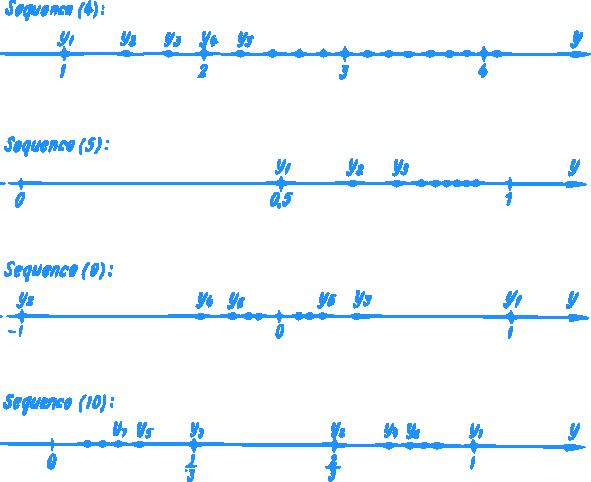
\includegraphics[width=0.9\textwidth]{figures/fig-06.pdf}
\caption{Mapping the sequences along a line.}
\label{fig-06}
\end{figure}

\rdr But in the case of sequences \eqref{series-04} and \eqref{series-05} the seond method looks rather obvious.

\athr It can be explained by specific features of those sequences. Look at them closer.

\rdr The terms of sequences  \eqref{series-04} and \eqref{series-05} possess the following property: each term is greater than the preceding term
\begin{equation*}%
y_{1} < y_{2} < y_{3}, \ldots < y_{n} < \ldots
\end{equation*}
It means that all the terms are arranged on the $y$-axis according to their serial numbers. As far as I know, such sequence, are called \emph{increasing}.

\athr A more general case is that of \emph{non-decreasing} sequences provided we add the equality sign to the above series of inequalities.
\begin{mytheo}{Definition}
A sequence ($y_{n}$) is called nondecreasing if
\begin{equation*}%
y_{1} \leqslant y_{2} \leqslant y_{3}, \ldots \leqslant y_{n} \leqslant \ldots
\end{equation*}
A sequence ($y_{n}$) is called non-increasing if
\begin{equation*}%
y_{1} \geqslant y_{2} \geqslant y_{3}, \ldots \geqslant y_{n} \geqslant \ldots
\end{equation*}
Non-decreasing and non-increasing sequences come under the name of monotonic sequences.
\end{mytheo}
Please, identify monotonic sequences among examples \eqref{series-01} -\eqref{series-13}.

\rdr Sequences \eqref{series-01}, \eqref{series-02}, \eqref{series-03}, \eqref{series-04}, \eqref{series-05}, \eqref{fibonacci}, \eqref{series-12}, and \eqref{series-13} are nondecreasing, while \eqref{series-06} and \eqref{series-07} are non-increasing. Sequences \eqref{series-08}, \eqref{series-09}, and \eqref{series-10} are not monotonic.

\athr Let us formulate one more definition.
\begin{mytheo}{Definition}
A sequence ($y_{n}$) is bounded if there are two numbers $A$ and $B$
labelling the range which encloses all the terms of a sequence
\begin{equation*}%
A \leqslant y_{n} \leqslant B \,\, (n = 1, \, 2, \, 3, \, \ldots)
\end{equation*}
\end{mytheo}

If it is impossible to identify such two numbers (or, in particular, one can find only one of the two such numbers, either the least or the greatest), such a sequence is \emph{unbounded}. Do you find bounded sequences among our examples? 

\rdr Apparently, \eqref{series-05} is bounded. 

\athr Find the numbers $A$ and $B$ for it.

\rdr $A=1/2, \, B= 1$.

\athr Of course, but if there exists even one pair of $A$ and $B$, one may find any number of such pairs. You could say, for example, that $A= 0, \, B= 2$, or $A=-100, \, B = 100$, etc., and be equally right.

\rdr Yes, but my numbers are more accurate.

\athr From the viewpoint of the bounded sequence definition, my numbers $A$ and $B$ are not Letter and not worse than yours. However, your last sentence is peculiar. What do you mean by saying ``more accurate?''

\rdr My $A$ is apparently the greatest of all possible lower bounds, while my $B$ is the least of all possible upper hounds.

\athr The first part of your statement is doubtlessly correct, while the second part of it, concerning $B$, is not so self-explanatory. It needs proof.

\rdr But it seemed	rather obvious. Because all the terms of \eqref{series-05} increase gradually, and evidently tend to unity, always remaining less than unity.

\athr Well, it is right. But it is not yet evident that $B = 1$ is the least number for which $y_{n} \leqslant B$ is valid for all $n$: I stress the point again: your statement is not self-evident, it needs proof.

I shall note also that ``self-evidence'' of your statement about $B = 1$ is nothing but your subjective impression; it is not a mathematically substantiated corollary.


\rdr But how to prove that $B = 1$ is, in this particular case, the least of all possible upper bounds?

\athr Yes, it can be proved. But let us not move too fast and by all means beware of excessive reliance on so-called self-evident impressions. The warning becomes even more important in the light of the fact that the bounded- ness of a sequence does not imply at all that the greatest $A$ or the least $B$ must be known explicitly.

Now, let us get back to our sequences and find other examples of bounded sequences.	 .

\rdr Sequence \eqref{series-07} is also bounded (one can easily find $A = 0, \, B = 1$). Finally, bounded sequences are \eqref{series-09} (e.g. $A=-1, \,B= 1$), \eqref{series-10} (e.g. $A=0, \, B= 1$), and \eqref{series-13} (e.g. $A = 3, \, B = 4$). The remaining' sequences are un-bounded.

\athr You are quite right. Sequences \eqref{series-05}, \eqref{series-07}, \eqref{series-09}, \eqref{series-10}, and \eqref{series-13} are bounded. Note that \eqref{series-05}, \eqref{series-07}, and \eqref{series-13} are bounded and at the same time monotonic. Don't you feel that this fact is somewhat puzzling?

\rdr What's puzzling about it?

\athr Consider, for example, sequence \eqref{series-05}. Note that each subsequent term is greater than the preceding one. I repeat, each term! But the sequence contains an infinite number of terms. Hence, if we follow the sequence far enough, we shall see as many terms with increased magnitude (compared to the preceding term) as we wish. Nevertheless, these values will never go beyond a certain ``boundary'', which in this case is unity. Doesn't it puzzle you?

\rdr Well, generally speaking, it does. But I notice that we add to each preceding term an increment which gradually becomes less and less.

\athr Yes, it is true. But this condition is obviously insufficient to make such a sequence bounded. Take, for example, sequence \eqref{series-04}. Here again the ``increments'' added to each term of the sequence gradually decrease; nevertheless, the sequence is not bounded.

\rdr We must conclude, therefore, that in \eqref{series-05} these ``increments'' diminish faster than in \eqref{series-04}.

\athr All the same, you have to agree that it is not immediately clear that these ``increments'' may decrease at a rate resulting in the boundedness of a sequence.

\rdr Of course, I agree with that.

\athr The possibility of infinite but bounded sets was not known, for example, to ancient Greeks. Suffice it to recall the famous paradox about Achilles chasing a turtle.

Let us assume that Achilles and the turtle are initially separated by a distance of \SI{1}{\kilo\meter}, Achilles moves to times faster than the turtle. Ancient Greeks reasoned like this: during the time Achilles covers \SI{1}{\kilo\meter} the turtle covers \SI{100}{\meter}. By the time Achilles has covered these \SI{100}{\meter}, the turtle will have made another \SI{10}{\meter}, and before Achilles has covered these \SI{10}{\meter}, the turtle will have made \SI{1}{\meter} more, and so on. Out of these considerations a paradoxical conclusion was derived that Achilles could never catch up with the turtle.

This ``paradox'' shows that ancient Greeks failed to grasp the fact that a monotonic sequence may be bounded.

\rdr One has to agree that the presence of both the monotonicity and boundedness is something not so simple to understand.

\athr Indeed, this is not so simple. It brings us close to a discussion on the limit of sequence. The point is that if a sequence is both monotonic and bounded, it should necessarily have a limit.

Actually, this point can be considered as the ``beginning'' of calculus.
}
% !TEX root = calculus.tex

\chapter{LIMIT OF SEQUENCE}
\label{dialogue-02}
{\parindent=0pt
\athr What mathematical operations do you know?

\rdr Addition, subtraction, multiplication, division, involution (raising to a power), evolution (extracting n root), and taking a logarithm or a modulus.

\athr In order to pass from elementary mathematics to higher mathematics, this ``list'' should be supplemented with one more mathematical operation, namely, that of finding the limit of sequence; this operation is called sometimes the limit transition (or passage to the limit). By the way, we shall clarify below the meaning of the last phrase of the previous dialogue, stating that calculus ``begins'' where the limit of sequence is introduced. 

\rdr I heard that higher mathematics uses the operations of \emph{differentiation} and \emph{integration}. 

\athr These operations, as we shall see, are in essence nothing but the variations of the limit transition. 

Now, let us get down to the concept of the \emph{limit of sequence}. Do you know what it is? 

\rdr I learned the definition of the limit of sequence. However, I doubt that I can reproduce it from memory. 

\athr But you seem to ``feel'' this notion somehow? Probably, you can indicate which of the sequences discussed above have limits and what the value of the limit is in each case. 

\rdr I think I can do this, The limit is 1 for sequence \eqref{series-05}, zero for \eqref{series-07} and \eqref{series-09}, and $\pi$ for \eqref{series-13}. 

\athr That's right. The remaining sequences have no limits.

\rdr By the way, sequence \eqref{series-09} is not monotonic \ldots

\athr Apparently, you have just remembered the end of our previous dialogue where it was stated that if a sequence is both monotonic and bounded, it has a limit.

\rdr That's correct. But isn't this a contradiction?

\athr Where do you find the contradiction? Do you think that from the statement ``If a sequence is both monotonic and bounded, it has a limit'' one should necessarily draw a reverse statement like ``If a sequence has a limit, it must be monotonic and bounded?'' Later we shall see that a necessary condition for a limit is only the boundedness of a sequence. The monotonicity is not mandatory at all; consider, for example, sequence \eqref{series-09}.

Let us get back to the concept of the limit of sequence. Since you have correctly indicated the sequences that have limits, you obviously have some understanding of this concept. Could you formulate it?

\rdr A limit is a number to which a given sequence tends (converges).

\athr What do you mean by saying ``converges to a number''?

\rdr I mean that with an increase of the serial number, the terms of a sequence converge very closely to a certain value.

\athr What do you mean by saying ``very closely''?

\rdr Well, the ``difference'' between the values of the terms and the given number will become infinitely small. Do you think any additional explanation is needed?

\athr The definition of the limit of sequence which you have suggested can at best be classified as a subjective impression. We have already discussed a similar situation in the previous dialogue.

Let us see what is hidden behind the statement made above. For this purpose, let us look at a rigorous definition of the limit of sequence which we are going to examine in detail.
\begin{mytheo}{Definition}
The number $a$ is said to be the limit of sequence ($y_{n}$) if for any positive number $\varepsilon$ there is a real number $N$ such that for all $ n > N$ the following inequality holds:
\begin{equation}%
| \, y_{n} - a \, | < \varepsilon
\label{limit-of-seq}
\end{equation}
\end{mytheo}

\rdr I am afraid, it is beyond me to remember such a definition.

\athr Don't hasten to remember. Try to comprehend this definition, to realize its structure and its inner logic. You will see that every word in this phrase carries a definite and necessary content and that no other definition of the limit of sequence could be more succinct (more delicate, even). 

First of all, let us note the logic of the sentence. A certain number is the limit provided that for any $\varepsilon > 0$ \emph{there is} a number $N$ such that for all $n > N$ inequality \eqref{limit-of-seq} holds. In short, it is necessary that for any $\varepsilon$ a certain number $N$ should exist.

Further, note two ``delicate'' aspects in this sentence. First, the number $N$ should exist for any positive number $\varepsilon$. Obviously, \emph{there is} an infinite set of such $\varepsilon$. Second, inequality \eqref{limit-of-seq} should hold always (i.e. for each $\varepsilon$) for \emph{all} $n > N$. But there is an equally infinite set of numbers n!

\rdr Now, the definition of the limit has become more obscure.

\athr Well, it is natural. So far we have been examining the definition ``piece by piece''. It is very important that the ``delicate'' features, the ``cream'', so to say, are spotted from the very outset. Once you understand them, everything will fall into place.

In \fig{fig-07}\textcolor{IndianRed}{(a)} there is a graphic image of a sequence. Strictly speaking, the first 40 terms have been plotted on the graph. Let us assume that if any regularity is noted in these 40 terms, we shall conclude that the regularity does exist for $n > 40$.

\begin{figure}[!h]
\centering
{\noindent
\begin{tikzpicture}[line cap=round,line join=round,>=triangle 45,x=0.2cm,y=0.3cm]
\foreach \x in {0,10,20,30,40}
\draw[shift={(\x,-4)},color=black] (0pt,2pt) -- (0pt,-2pt) node[below] {\footnotesize $\x$};
%\draw[color=black] (0pt,-10pt) node[right] {\footnotesize $0$};
\clip(-5.5,-6) rectangle (52,6);
\foreach \x in {1,...,40}
\draw [line width=.75pt,dash pattern=on 5pt off 5pt,color=DarkGray] (\x,4.)-- (\x,-4.);

\draw [line width=1pt,dash pattern=on 3pt off 3pt,color=IndianRed] (0.,0.)-- (42.,0.);
\draw [->,line width=1.2pt,color=DarkGray] (0.,-4.) -- (0.,5.348012295333778);
\draw [->,line width=1.2pt,color=DarkGray] (0.,-4.) -- (50,-4.);
\draw (-.5,4.5) node[left] {\footnotesize$y_{n}$};
\draw (0,0) node[left] {\footnotesize$a$};
\draw (48,-4.028170894118617) node[below] {\footnotesize$n$};
\begin{scriptsize}
\draw (-2.8,-4) node[left] {\normalsize \textit{ (a)}};
\filldraw [IndianRed] (0.,0.) circle (1.5pt);
\filldraw [IndianRed] (1.,-3.24098) circle (1.5pt);
\filldraw [IndianRed] (2.,3.49351) circle (1.5pt);
\filldraw [IndianRed] (3.,-3.24098) circle (1.5pt);
\filldraw [IndianRed] (4.,1.92) circle (1.5pt);
\filldraw [IndianRed] (5.,0.) circle (1.5pt);
\filldraw [IndianRed] (6.,2.84361) circle (1.5pt);
\filldraw [IndianRed] (7.,-3.1191) circle (1.5pt);
\filldraw [IndianRed] (8.,2.53306) circle (1.5pt);
\filldraw [IndianRed] (9.,-2.5808) circle (1.5pt);
\filldraw [IndianRed] (10.,1.19082) circle (1.5pt);
\filldraw [IndianRed] (11.,2.11898) circle (1.5pt);
\filldraw [IndianRed] (13.,2.05687) circle (1.5pt);
\filldraw [IndianRed] (12.,-2.97418) circle (1.5pt);
\filldraw [IndianRed] (14.053794841260318,-1.0487146075110734) circle (1.5pt);
\filldraw [IndianRed] (16.,1.04238) circle (1.5pt);
\filldraw [IndianRed] (15.,-1.87687) circle (1.5pt);
\filldraw [IndianRed] (17.,-1.66983) circle (1.5pt);
\filldraw [IndianRed] (18.,-0.59323) circle (1.5pt);
\filldraw [IndianRed] (19.,0.) circle (1.5pt);
\filldraw [IndianRed] (20.,1.39434) circle (1.5pt);
\filldraw [IndianRed] (21.,0.77323) circle (1.5pt);
\filldraw [IndianRed] (22.,-1.54561) circle (1.5pt);
\filldraw [IndianRed] (23.,-0.67604) circle (1.5pt);
\filldraw [IndianRed] (24.,0.56619) circle (1.5pt);
\filldraw [IndianRed] (25.,1.35294) circle (1.5pt);
\filldraw [IndianRed] (26.,0.) circle (1.5pt);
\filldraw [IndianRed] (27.,-1.06942) circle (1.5pt);
\filldraw [IndianRed] (28.,0.52478) circle (1.5pt);
\filldraw [IndianRed] (29.,-0.51041) circle (1.5pt);
\filldraw [IndianRed] (30.,-0.51041) circle (1.5pt);
\filldraw [IndianRed] (31.,0.46267) circle (1.5pt);
\filldraw [IndianRed] (32.,0.44196) circle (1.5pt);
\filldraw [IndianRed] (33.,0.71112) circle (1.5pt);
\filldraw [IndianRed] (34.,-0.51041) circle (1.5pt);
\filldraw [IndianRed] (35.,0.25563) circle (1.5pt);
\filldraw [IndianRed] (36.,0.29704) circle (1.5pt);
\filldraw [IndianRed] (37.,-0.05493) circle (1.5pt);
\filldraw [IndianRed] (38.,-0.48971) circle (1.5pt);
\filldraw [IndianRed] (39.,0.25563) circle (1.5pt);
\filldraw [IndianRed] (40.,0.25563) circle (1.5pt);
\end{scriptsize}
\end{tikzpicture}
% part 2
\begin{tikzpicture}[line cap=round,line join=round,>=triangle 45,x=0.2cm,y=0.3cm]
\foreach \x in {0,10,20,30,40}
\draw[shift={(\x,-4)},color=black] (0pt,2pt) -- (0pt,-2pt) node[below] {\footnotesize $\x$};
%\draw[color=black] (0pt,-10pt) node[right] {\footnotesize $0$};
\clip(-5.5,-6) rectangle (52,6);
\foreach \x in {1,...,40}
\draw [line width=.75pt,dash pattern=on 5pt off 5pt,color=DarkGray] (\x,4.)-- (\x,-4.);
\draw [line width=.5pt,dash pattern=on 5pt off 5pt,color=DodgerBlue] (0.,2.8)-- (44.,2.8);
\draw [line width=.5pt,dash pattern=on 5pt off 5pt,color=DodgerBlue] (0.,-2.8)-- (44.,-2.8);
\draw [<->,line width=.75pt,color=DarkGray] (43,2.8)-- (43,-2.8);
\draw (43,0) node[right,color=black] {\footnotesize $2 \varepsilon$};
\draw (0.,2.8) node[left,color=black] {\footnotesize $a + \varepsilon$};
\draw (0.,-2.8) node[left,color=black] {\footnotesize $a - \varepsilon$};
\draw [line width=1pt,dash pattern=on 3pt off 3pt,color=IndianRed] (0.,0.)-- (42.,0.);
\draw [->,line width=1.2pt,color=DarkGray] (0.,-4.) -- (0.,5.348012295333778);
\draw [->,line width=1.2pt,color=DarkGray] (0.,-4.) -- (50,-4.);
\draw (-.5,4.5) node[left] {\footnotesize $y_{n}$};
\draw (0,0) node[left] {\footnotesize $a$};
\draw (48,-4) node[below] {\footnotesize $n$};
\begin{scriptsize}
\draw (-2.8,-4) node[left] {\normalsize \textit{(b)}};
\filldraw [IndianRed] (0.,0.) circle (1.5pt);
\filldraw [IndianRed] (1.,-3.24098) circle (1.5pt);
\filldraw [IndianRed] (2.,3.49351) circle (1.5pt);
\filldraw [IndianRed] (3.,-3.24098) circle (1.5pt);
\filldraw [IndianRed] (4.,1.92) circle (1.5pt);
\filldraw [IndianRed] (5.,0.) circle (1.5pt);
\filldraw [IndianRed] (6.,2.84361) circle (1.5pt);
\filldraw [IndianRed] (7.,-3.1191) circle (1.5pt);
\filldraw [IndianRed] (8.,2.53306) circle (1.5pt);
\filldraw [IndianRed] (9.,-2.5808) circle (1.5pt);
\filldraw [IndianRed] (10.,1.19082) circle (1.5pt);
\filldraw [IndianRed] (11.,2.11898) circle (1.5pt);
\filldraw [IndianRed] (13.,2.05687) circle (1.5pt);
\filldraw [IndianRed] (12.,-2.97418) circle (1.5pt);
\filldraw [IndianRed] (14.053794841260318,-1.0487146075110734) circle (1.5pt);
\filldraw [IndianRed] (16.,1.04238) circle (1.5pt);
\filldraw [IndianRed] (15.,-1.87687) circle (1.5pt);
\filldraw [IndianRed] (17.,-1.66983) circle (1.5pt);
\filldraw [IndianRed] (18.,-0.59323) circle (1.5pt);
\filldraw [IndianRed] (19.,0.) circle (1.5pt);
\filldraw [IndianRed] (20.,1.39434) circle (1.5pt);
\filldraw [IndianRed] (21.,0.77323) circle (1.5pt);
\filldraw [IndianRed] (22.,-1.54561) circle (1.5pt);
\filldraw [IndianRed] (23.,-0.67604) circle (1.5pt);
\filldraw [IndianRed] (24.,0.56619) circle (1.5pt);
\filldraw [IndianRed] (25.,1.35294) circle (1.5pt);
\filldraw [IndianRed] (26.,0.) circle (1.5pt);
\filldraw [IndianRed] (27.,-1.06942) circle (1.5pt);
\filldraw [IndianRed] (28.,0.52478) circle (1.5pt);
\filldraw [IndianRed] (29.,-0.51041) circle (1.5pt);
\filldraw [IndianRed] (30.,-0.51041) circle (1.5pt);
\filldraw [IndianRed] (31.,0.46267) circle (1.5pt);
\filldraw [IndianRed] (32.,0.44196) circle (1.5pt);
\filldraw [IndianRed] (33.,0.71112) circle (1.5pt);
\filldraw [IndianRed] (34.,-0.51041) circle (1.5pt);
\filldraw [IndianRed] (35.,0.25563) circle (1.5pt);
\filldraw [IndianRed] (36.,0.29704) circle (1.5pt);
\filldraw [IndianRed] (37.,-0.05493) circle (1.5pt);
\filldraw [IndianRed] (38.,-0.48971) circle (1.5pt);
\filldraw [IndianRed] (39.,0.25563) circle (1.5pt);
\filldraw [IndianRed] (40.,0.25563) circle (1.5pt);
\end{scriptsize}
\end{tikzpicture}
% part 3
\begin{tikzpicture}[line cap=round,line join=round,>=triangle 45,x=0.2cm,y=0.3cm]
\foreach \x in {0,10,20,30,40}
\draw[shift={(\x,-4)},color=black] (0pt,2pt) -- (0pt,-2pt) node[below] {\footnotesize $\x$};
%\draw[color=black] (0pt,-10pt) node[right] {\footnotesize $0$};
\clip(-5.5,-6) rectangle (52,6);
\foreach \x in {1,...,40}
\draw [line width=.75pt,dash pattern=on 5pt off 5pt,color=DarkGray] (\x,4.)-- (\x,-4.);
\draw [line width=1pt,dash pattern=on 3pt off 3pt,color=IndianRed] (0.,0.)-- (42.,0.);
\draw [->,line width=1.2pt,color=DarkGray] (0.,-4.) -- (0.,5.348012295333778);
\draw [->,line width=1.2pt,color=DarkGray] (0.,-4.) -- (50,-4.);
\draw (-.5,4.5) node[left] {\footnotesize$y_{n}$};
\draw (0,0) node[left] {\footnotesize$a$};
\draw [line width=.5pt,dash pattern=on 5pt off 5pt,color=DodgerBlue] (7.,2)-- (50.,2);
\draw [line width=.5pt,dash pattern=on 5pt off 5pt,color=DodgerBlue] (7.,-2)-- (50.,-2);
\draw [line width=.5pt,dash pattern=on 5pt off 5pt,color=DodgerBlue] (15.,1.2)-- (47.,1.2);
\draw [line width=.5pt,dash pattern=on 5pt off 5pt,color=DodgerBlue] (15.,-1.2)-- (47.,-1.2);
\draw [line width=.5pt,dash pattern=on 5pt off 5pt,color=DodgerBlue] (27.,.5)-- (43.,.5);
\draw [line width=.5pt,dash pattern=on 5pt off 5pt,color=DodgerBlue] (27.,-.5)-- (43.,-.5);
\draw (48,-4.028170894118617) node[below] {\footnotesize$n$};
\draw [<->,line width=.75pt,color=DarkGray] (49,2)-- (49,-2);
\draw [<->,line width=.75pt,color=DarkGray] (46,1.2)-- (46,-1.2);
\draw (49,0) node[right,color=black] {\footnotesize $2 \varepsilon_{1}$};
\draw (46,0) node[right,color=black] {\footnotesize $2 \varepsilon_{2}$};
\draw (42,0) node[right,color=black] {\footnotesize $2 \varepsilon_{3}$};
\begin{scriptsize}
\draw (-2.8,-4) node[left] {\normalsize \textit{(c)}};
\filldraw [IndianRed] (0.,0.) circle (1.5pt);
\filldraw [IndianRed] (1.,-3.24098) circle (1.5pt);
\filldraw [IndianRed] (2.,3.49351) circle (1.5pt);
\filldraw [IndianRed] (3.,-3.24098) circle (1.5pt);
\filldraw [IndianRed] (4.,1.92) circle (1.5pt);
\filldraw [IndianRed] (5.,0.) circle (1.5pt);
\filldraw [IndianRed] (6.,2.84361) circle (1.5pt);
\filldraw [IndianRed] (7.,-3.1191) circle (1.5pt);
\filldraw [IndianRed] (8.,2.53306) circle (1.5pt);
\filldraw [IndianRed] (9.,-2.5808) circle (1.5pt);
\filldraw [IndianRed] (10.,1.19082) circle (1.5pt);
\filldraw [IndianRed] (11.,2.11898) circle (1.5pt);
\filldraw [IndianRed] (13.,2.05687) circle (1.5pt);
\filldraw [IndianRed] (12.,-2.97418) circle (1.5pt);
\filldraw [IndianRed] (14.053794841260318,-1.0487146075110734) circle (1.5pt);
\filldraw [IndianRed] (16.,1.04238) circle (1.5pt);
\filldraw [IndianRed] (15.,-1.87687) circle (1.5pt);
\filldraw [IndianRed] (17.,-1.66983) circle (1.5pt);
\filldraw [IndianRed] (18.,-0.59323) circle (1.5pt);
\filldraw [IndianRed] (19.,0.) circle (1.5pt);
\filldraw [IndianRed] (20.,1.39434) circle (1.5pt);
\filldraw [IndianRed] (21.,0.77323) circle (1.5pt);
\filldraw [IndianRed] (22.,-1.54561) circle (1.5pt);
\filldraw [IndianRed] (23.,-0.67604) circle (1.5pt);
\filldraw [IndianRed] (24.,0.56619) circle (1.5pt);
\filldraw [IndianRed] (25.,1.35294) circle (1.5pt);
\filldraw [IndianRed] (26.,0.) circle (1.5pt);
\filldraw [IndianRed] (27.,-1.06942) circle (1.5pt);
\filldraw [IndianRed] (28.,0.52478) circle (1.5pt);
\filldraw [IndianRed] (29.,-0.51041) circle (1.5pt);
\filldraw [IndianRed] (30.,-0.51041) circle (1.5pt);
\filldraw [IndianRed] (31.,0.46267) circle (1.5pt);
\filldraw [IndianRed] (32.,0.44196) circle (1.5pt);
\filldraw [IndianRed] (33.,0.71112) circle (1.5pt);
\filldraw [IndianRed] (34.,-0.51041) circle (1.5pt);
\filldraw [IndianRed] (35.,0.25563) circle (1.5pt);
\filldraw [IndianRed] (36.,0.29704) circle (1.5pt);
\filldraw [IndianRed] (37.,-0.05493) circle (1.5pt);
\filldraw [IndianRed] (38.,-0.48971) circle (1.5pt);
\filldraw [IndianRed] (39.,0.25563) circle (1.5pt);
\filldraw [IndianRed] (40.,0.25563) circle (1.5pt);
\end{scriptsize}
\end{tikzpicture}
}
%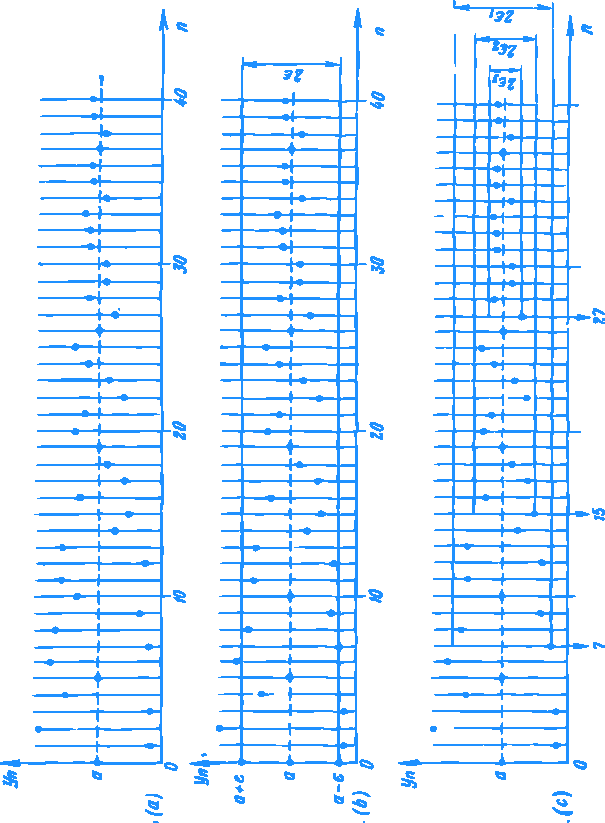
\includegraphics[width=0.9\textwidth]{figures/fig-07.pdf}
\caption{Finding limit of a sequence.}
\label{fig-07}
\end{figure}

Can we say that this sequence converges to the number $a$ (in other words, the number $a$ is the limit of the sequence)?

\rdr It seems plausible.

\athr Let us however, act not on the basis of our impressions but on the basis of the definition of the limit of sequence. So, we want to verify whether the number $a$ is the limit of the given sequence. What does our definition of the limit prescribe us to do?

\rdr We should take a positive number $\varepsilon$. 

\athr Which number? 

\rdr Probably. it must be small enough,

\athr The words ``small enough'' are neither here nor there. The number $\varepsilon$ must be arbitrary.

Thus, we take an arbitrary positive $\varepsilon$. Let us have a look at  \fig{fig-07}and layoff on the $y$-axis an interval of length $\varepsilon$, both upward and downward from the same point $a$. Now, let us draw through the points $y = a + \varepsilon$ and $y = a - \varepsilon$ the horizontal straight lines that mark an ``allowed'' band for our sequence. If for any term of the sequence inequality \eqref{limit-of-seq} holds, the points on the graph corresponding to these terms fall inside the ``allowed'' band. We see  in \fig{fig-07}\textcolor{IndianRed}{(b)} that starting from number $\varepsilon$, all the terms of the sequence stay within the limits of the ``allowed'' band, proving the validity of \eqref{limit-of-seq} for these terms. We, of course, assume that this situation will realize for all $n > 40$, i.e. for the whole infinite ``tail'' of the sequence not shown in the diagram.

Thus, for the selected $\varepsilon$ the number $N$ does exist. In this particular case we found it to be 7.


\rdr Hence, we can regard $a$ as the limit of the sequence.

\athr Don't you hurry. The definition clearly emphasizes: ``for \emph{any} positive $\varepsilon$''. So far we have analyzed only one value of $\varepsilon$. We should take another value of $\varepsilon$ and find $N$ not for a larger but for a smaller $\varepsilon$. If for the second $\varepsilon$ the search of $N$ is a success, we should take a third, even smaller $\varepsilon$, and then a fourth, still smaller $\varepsilon$, etc., repeating each time the operation of finding $N$.

In   \fig{fig-07}\textcolor{IndianRed}{(c)} three situations are drawn up for  $\varepsilon_{1}, \varepsilon_{2}$and $\varepsilon_{3}$ (in this case $\varepsilon_{1} > \varepsilon_{2} > \varepsilon_{3}$). Correspondingly, three ``allowed'' bands are plotted on the graph. For a greater clarity, each of these bands has its own starting $N$. We have chosen $N_{1}=7, \, N_{2} =15$, and $N_{3}=27$. 

Note that for each selected $\varepsilon$ we observe the same situation in  \fig{fig-07}\textcolor{IndianRed}{(c)}: up to a certain $n$, the sequence, speaking figuratively, may be ``indisciplined'' (in other words, some terms may fallout of the limits of the corresponding ``allowed'' band). However, after a certain $n$ is reached, a very rigid law sets in, namely, \emph{all the remaining terms of the sequence} (their number is infinite) \emph{do stay within the band}.

\rdr Do we really have to check it for an infinite number of $\varepsilon$ values?

\athr Certainly not. Besides, it is impossible. We must be sure that \emph{whichever} value of $\varepsilon > 0$ we take, there is such $N$ after which the whole infinite ``tail'' of the sequence will get ``locked up'' within the limits of the corresponding ``allowed'' band.

\rdr And what if we are not so sure?

\athr If we are not and if one can find a value of $\varepsilon_{1}$ such that it is impossible to ``lock up'' the infinite ``tail'' of the sequence within the limits of its ``allowed'' hand, then a is not the limit of our sequence.

\rdr And when do we reach the certainty?

\athr We shall talk this matter over at a later stage because it has nothing to do with the essence of the definition of the limit of sequence.
I suggest that you formulate this definition anew. Don't try to reconstruct the wording given earlier, just try to put it in your own words.

\rdr I'll try. The number $a$ is the limit of a given sequence if for any positive $\varepsilon$ there is (one can find) a serial number $n$ such that for all subsequent numbers (i.e. for the whole infinite ``tail'' of the sequence) the following inequality holds: $| \, y_{n} - a \, | < \varepsilon$.

\athr Excellent. You have almost repeated word by word the definition that seemed to you impossible to remember.

\rdr Yes, in reality it all has turned out to be quite logical and rather easy.

\athr It is worthwhile to note that the dialectics of thinking was clearly at work in this case: a concept becomes ``not difficult'' because the ``complexities'' built into it were clarified. First, we break up the concept into fragments, expose the ``complexities'', then examine the ``delicate'' points, thus trying to reach the ``core'' of the problem. Then we recompose the concept to make it integral, and, as a result, this reintegrated concept becomes sufficiently simple and comprehensible. In the future we shall try first to find the internal structure and internal logic of the concepts and theorems.

I believe we can consider the concept of the limit of sequence as thoroughly analyzed. I should like to add that, as a result, the meaning of the sentence ``the sequence converges to $a$'' has been explained. I remind you that initially
this sentence seemed to you as requiring no additional explanations.

\rdr At the moment it does not seem so self-evident any more. True, I see 
now quite clearly the idea behind it.

\athr Let us get back to examples  \eqref{series-05}, \eqref{series-07}, and  \eqref{series-09}. Those are the sequences that we discussed at the beginning of our talk. To begin with, we note that the fact that a sequence ($y_{n}$) converges to a certain number $a$ is conventionally written as
\begin{equation*}%
\lim\limits_{n \to \infty} y_{n}= a	
\end{equation*}
(it reads like this: ``The limit of $y_{n}$ for $n$ tending to infinity is $a$.'')

Using the definition of the limit, let us prove that 
\begin{equation*}%
\begin{split}
\lim\limits_{n \to \infty} \dfrac{n}{n+1} = 1; \quad \lim\limits_{n \to \infty} \frac{1}{n}= 0;\\
\lim\limits_{n \to \infty} \left\{ \frac{1}{2n} [1 - (-1)^{n}] - \frac{1}{2(n-1)}  [1 + (-1)^{n}] \right\} =0
\end{split}
\end{equation*}
You will begin with the first of the above problems. 

\rdr I have to prove that
\begin{equation*}%
\lim\limits_{n \to \infty} \dfrac{n}{n+1} = 1
\end{equation*}
I choose an arbitrary value of $\varepsilon$, for example, $\varepsilon = 0.1$. 

\athr I advise you to begin with finding the modulus
of $| y_{n}- a|$. 

\rdr In this case, the-modulus is
\begin{equation*}%
\left| \dfrac{n}{n+1} - 1 \right| = \dfrac{1}{n+1} 
\end{equation*}

\athr Apparently $\varepsilon$ needn't be specified, at least at the beginning.

\rdr O.K. Therefore. for an arbitrary positive value of $\varepsilon$, I have to find $N$ such that for all $n > N$ the following inequality holds
\begin{equation*}%
\dfrac{1}{n+1} < \varepsilon
\end{equation*}

\athr Quite correct. Go on.

\rdr The inequality can be rewritten in the form t
\begin{equation*}%
n > \dfrac{1}{\varepsilon} - 1 
\end{equation*}
It follows that the unknown $N$ may be identified as an integral part of $\dfrac{1}{\varepsilon} -	1$. Apparently, for all $n > N$ the inequality in question will hold. 

\athr That's right. Let, for example, $\varepsilon = 0.01$. 

\rdr Then $N = \dfrac{1}{\varepsilon} - 1 = 100 - 1 = 99$.

\athr Let $\varepsilon  = 0.001$.

\rdr Then $N = \dfrac{1}{\varepsilon} - 1 = 1000 - 1 = 999$.

\athr Let $\varepsilon  = 0.00015$.

\rdr Then $N = \dfrac{1}{\varepsilon} - 1 = 6665$.

\athr It is quite evident that for any $\varepsilon$ (no matter how small) we can find a corresponding $N$.

As to proving that the limits of sequences \eqref{series-07} and \eqref{series-09} are zero, we shall leave it to the reader as an exercise.

\rdr But couldn't the proof of the equality $\lim\limits_{n \to \infty} \dfrac{n}{n+1} = 1$ be simplified?

\athr Have a try.

\rdr Well, first I rewrite the expression in the following way:
\begin{equation*}%
\lim\limits_{n \to \infty} \dfrac{n}{n+1} = \lim\limits_{n \to \infty} \dfrac{1}{\dfrac{1}{n+1}}
\end{equation*}
Then I take into consideration that with an increase in $n$, fraction $\dfrac{1}{n}$ will tend to zero, and, consequently, can be neglected against unity. Hence, we may reject $\dfrac{1}{n}$ and have:  $ \lim\limits_{n \to \infty} \dfrac{1}{1} = 1 $.

\athr In practice this is the method generally used. However	one should note that in this case we have assumed,
first, that $ \lim\limits_{n \to \infty} \dfrac{1}{n} = 0 $, and, second, the validity of the following rules
\begin{align}%
\lim\limits_{n \to \infty} \frac{x_{n}}{y_{n}} & = \frac{\lim\limits_{n \to \infty} x_{n}}{\lim\limits_{n \to \infty} y_{n}} \label{lim-div}\\
\lim\limits_{n \to \infty} (x_{n} + z_{n}) & =\lim\limits_{n \to \infty} x_{n} + \lim\limits_{n \to \infty} z_{n} \label{lim-sum}
\end{align} 
where $x_{n} =1, \, y_{n} = 1 + \dfrac{1}{n}$ and $z_{n} = \dfrac{1}{n}$. Later on we shall discuss these rules, but at this juncture I suggest that we simply use them to compute several limits. Let us discuss two examples.	

\textcolor{IndianRed}{\bf Example 1} Find $ \lim\limits_{n \to \infty} \dfrac{3n - 1}{5n - 6} $.

\rdr It will be convenient to present the computation in the form:
\begin{align*}%
\lim\limits_{n \to \infty} \dfrac{3n - 1}{5n - 6} & = \lim\limits_{n \to \infty} \dfrac{3 - \dfrac{1}{n}}{5 - \dfrac{6}{n}} \\
& = \dfrac{\lim\limits_{n \to \infty} \left(3 - \dfrac{1}{n}\right)}{\lim\limits_{n \to \infty} \left(5 - \dfrac{6}{n}\right)}
= \dfrac{3}{5}
\end{align*} 
\athr Ok. \textcolor{IndianRed}{\bf Example 2} Compute
\begin{equation*}%
\lim\limits_{n \to \infty} \dfrac{6n^{2} - 1}{5n^{2} +2n -1} 
\end{equation*}
\rdr We write
\begin{equation*}%
\lim\limits_{n \to \infty} \dfrac{6n^{2} - 1}{5n^{2} +2n -1}  = \lim\limits_{n \to \infty} \dfrac{6n - \dfrac{1}{n}}{5n +2 - \dfrac{1}{n}}.
\end{equation*}

\athr Wait a moment! Did you think about the reason for dividing both the numerator and denominator of the fraction in the previous example by $n$? We did this because sequences $(3 n - 1)$ and $(5n -	6)$	obviously have no limits, and therefore rule \eqref{lim-div} fails. However, each of
sequences $\left( 3 - \dfrac{1}{n} \right)$ and $\left( 5 - \dfrac{6}{n} \right)$ has a limit.

\rdr I have got your point. It means that in \textcolor{IndianRed}{\bf Example 2} I have to divide both the numerator and denominator by $n^{2}$ to obtain the sequences with limits in both. Accordingly we obtain
\begin{align*}%
\lim\limits_{n \to \infty} \dfrac{6n^{2} - 1}{5n^{2} +2n -1}  & = \lim\limits_{n \to \infty} \dfrac{6 - \dfrac{1}{n^{2}}}{5 + \dfrac{2}{n} - \dfrac{1}{n^{2}}} \\
& = \frac{\lim\limits_{n \to \infty} \left( 6 - \dfrac{1}{n^{2}}\right) }{\lim\limits_{n \to \infty} \left( 5 + \dfrac{2}{n	} - \dfrac{1}{n^{2}}\right)}
\end{align*}


\athr Well, we have examined the concept of the limit of sequence. Moreover, we have learned a little how to calculate limits. Now it is time to discuss some properties of sequences with limits. Such sequences are called \emph{convergent}.
}
% !TEX root = calculus.tex

\chapter{CONVERGENT SEQUENCE}
\label{conv-seq}
{\parindent=0pt
\athr Let us prove the following theorem: 
\begin{mytheo}{Theorem}
If a sequence has a limit, it is bounded.
\label{limit-bound}
\end{mytheo}
We assume that $a$ is the limit of a sequence ($y_{n}$). Now take an arbitrary value of $\varepsilon$ greater than 0. According to the definition of the limit, the selected $\varepsilon$ can always be related to $N$ such that for all $n > N, \, Iy_{n} -a | < \varepsilon$ starting with $n = N + 1$, all the subsequent terms of the sequence satisfy the following inequalities
\begin{equation*}
a - \varepsilon < y_{n} < a + \varepsilon 
\end{equation*}
As to the terms with serial numbers from 1 to $N$, it is alway possible to select both the greatest (denoted by $B_{1}$ ) and the least (denoted by $A_{1}$) terms since the number of these term is \emph{finite}.

Now we have to select the least value from $a - \varepsilon$ and $A_{1}$ (denoted by $A$) and the greatest value from $a + \varepsilon$ and $B_{1}$ (denoted by $B$). It is obvious that $A \leqslant y_{n} \leqslant B$ for all the terms of our sequence, which proves that the sequence $y_{n}$ is bounded.

\rdr I see.

\athr Not too well, it seems. Let us have a look at the logical structure of the proof. We must verify that if the sequence has a limit, there exist two numbers $A$ and $B$ such that $A \leqslant y_{n} \leqslant B$ for each term of the sequence. Should the sequence contain a \emph{finite} number of terms, the existence of such two numbers would be evident. However, the sequence contains an \emph{infinite} number of terms, the fact that complicates the situation. 

\rdr Now it is clear! The point is that if a sequence has a limit $a$, one concludes that in the interval from $a - \varepsilon$ to $a + \varepsilon$ we have an infinite set of $y_{n}$ starting from $n = N +1$ so that \emph{outside of this interval} we shall find only a finite number of terms (not larger than $N$).

\athr Quite correct. As you see, the limit ``takes care of'' all the complications associated with the behaviour of the infinite ``tail'' of a sequence. Indeed, $| y_{n} - a | < \varepsilon$ for \emph{all} $n > N$, and this is the main ``delicate'' point of this theorem. As to the first $N$ terms of a sequence, it is essential that their set is finite.

\rdr Now it is all quite lucid. But what about $\varepsilon$ Its value is not preset, we have to select it.

\athr A selection of a value for $\varepsilon$ affects only $N$. If you	take a smaller $\varepsilon$,	you will get, generally speaking, a larger $N$. However, the number of the terms of a sequence which do not satisfy	$| y_{n} - a | < \varepsilon$ will remain finite.

And now try to answer the question about the validity of t.he converse theorem: If a sequence is bounded, does it imply it is convergent as well?

\rdr The converse theorem is not true. For example, sequence \eqref{series-10} which was discussed in the first dialogue is bounded. However, it has no limit.

\athr Right you are. We thus come to a corollary:
\begin{mytheo}{Corollary}
The boundedness of a sequence is a necessary condition for its convergence; however, it is not a sufficient condition. If a sequence is convergent, it is bounded. If a sequence is unbounded, it is definitely non-convergent,
\end{mytheo}

\rdr I wonder whether there is a sufficient condition for the convergence of a sequence?

\athr We have already mentioned this condition in the previous dialogue, namely, simultaneous validity of both the boundedness and monotonicity of a sequence. The \textbf{Weierstrass Theorem} states:
\begin{mytheo}{Weierstrass Theorem}
If a sequence is both bounded and monotonic, it has a limit.
\end{mytheo}
Unfortunately, the proof of the theorem is beyond the scope of this book; we shall not give it. I shall simply ask you to look again at sequences \eqref{series-05}, \eqref{series-07}, and \eqref{series-13} (see \hyperref[infinite-seq]{Dialogue One}), which satisfy the conditions of the Weierstrass theorem. 

\rdr As far as I understand, again the converse theorem is not true. Indeed, sequence \eqref{series-09} (from \hyperref[infinite-seq]{Dialogue One}) has a
limit but is not monotonic. 

\athr That is correct. We thus come to the following conclusion.
\begin{mytheo}{Conclusion}
If a sequence is both monotonic and bounded, it is a sufficient (but not necessary)	condition for its convergence.
\end{mytheo}

\rdr Well, one can easily get confused.

\begin{figure}[!h]
\centering
\begin{tikzpicture}[opacity=0.4]
  \filldraw [color=IndianRed=1.5,x radius=3cm, y radius=2cm](1,0) circle;
  \filldraw [color=DodgerBlue,radius=1.5,x radius=2.3cm, y radius=1cm](1,-1) circle;
  \filldraw [color=SteelBlue,radius=1.5,x radius=2cm, y radius=1.5cm,rotate=20](0,-2.5) circle;
\clip(0,-4) rectangle (6.2,2);
\draw (3,1.8) node[right,color=IndianRed,opaque] {\footnotesize \textit{Bounded Sequences}};
\draw (2.6,-2.8) node[right,color=SteelBlue,opaque] {\footnotesize \textit{Monotonic Sequences}};
\draw (3,-1.8) node[right,color=IndianRed] {\footnotesize \textit{Convergent Sequences}};
\draw (3,-1.8) node[right,color=DodgerBlue] {\footnotesize \textit{Convergent Sequences}};
\draw (1,-1.2) node[right,color=Black,opaque] {\footnotesize $A$};
  \filldraw [color=black,radius=0.8mm,opaque] (1,-1.2) circle;
\draw (1.4,-.4) node[right,color=Black,opaque] {\footnotesize $B$};
  \filldraw [color=black,radius=0.8mm,opaque](1.4,-.4) circle;
\draw (2,.5) node[right,color=Black,opaque] {\footnotesize $C$};
  \filldraw [color=black,radius=0.8mm,opaque](2,.5) circle;
\draw (1,-2.3) node[right,color=Black,opaque] {\footnotesize $D$};
  \filldraw [color=black,radius=0.8mm,opaque](1,-2.3)  circle;
\draw (2,-3.8) node[right,color=Black,opaque] {\footnotesize $E$};
  \filldraw [color=black,radius=0.8mm,opaque](2,-3.8) circle;
\end{tikzpicture}
%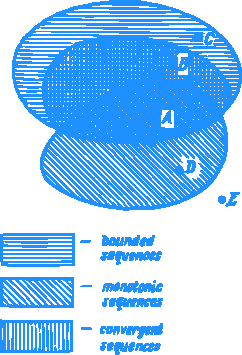
\includegraphics[width=0.4\textwidth]{figures/fig-08.pdf}
\caption{Bounded, monotonic and convergent sequences.}
\label{fig-08}
\end{figure}


\athr In order to avoid confusion, let us have a look at another illustration (\hyperref[fig-08]{Figure \ref{fig-08}}). Let us assume that all bounded sequences are ``collected'' (as if we were picking marbles scattered on the floor) in an area shaded by horizontal lines, all monotonic sequences are collected in an area shaded
by tilted lines, and, finally, all convergent sequences are collected in an area shaded by vertical lines. \hyperref[fig-08]{Figure \ref{fig-08}} shows how all these areas overlap, in accordance with the theorems discussed above (the actual shape of all the areas is, of course, absolutely arbitrary). As follows from the figure, the area shaded vertically is completely included into the area shaded horizontally. It means that \emph{any convergent sequence must be also bounded}. The overlapping of the areas shaded horizontally and by tilted lines occurs inside the area shaded vertically. It means that \emph{any sequence that is both bounded and monotonic must be convergent as well}. It is easy to deduce that only five types of sequences are possible. In the figure the points designated by $A, \, B, \, C, \, D$, and $E$ identify five sequences of different types. Try to name these sequences and find the corresponding examples among the sequences discussed in  \hyperref[infinite-seq]{Dialogue One}.

\rdr Point $A$ falls within the intersection of all the three areas. It represents a sequence which is at the same time bounded, monotonic, and convergent. Sequences \eqref{series-05}, \eqref{series-07}, and \eqref{series-13} are examples of such sequences.

\athr Continue, please.

\rdr Point $B$ represents a bounded, convergent hut non-monotonic sequence. One example is sequence \eqref{series-09}.

Point $C$ represents a bounded but neither convergent nor monotonic sequence. One example of such a sequence is sequence \eqref{series-10}.

Point $D$ represents a monotonic but neither convergent nor bounded sequence. Examples of such sequences are \eqref{series-01}, \eqref{series-02}, \eqref{series-03}, \eqref{series-04}, \eqref{series-06}, \eqref{fibonacci}, and \eqref{series-12}. 

Point $E$ is outside of the shaded areas and thus represents it sequence neither monotonic nor convergent nor bounded. One example is sequence \eqref{series-08}.

\athr What type of sequence is impossible then?

\rdr There can be no bounded, monotonic, and non-convergent sequence. Moreover, it is impossible to have both unboundedness and convergence in one sequence.

\athr As you see, \hyperref[fig-08]{Figure \ref{fig-08}} helps much to understand t.he relationship between such properties of sequences as \emph{boundedness, monotonicity, and convergence}.

In what follows, we shall discuss only convergent sequences.	We shall prove	the	following theorem:
\begin{mytheo}{Theorem}
A convergent sequence has only one limit.
\end{mytheo}
This is the theorem of the \emph{uniqueness of the limit}. It means that a convergent sequence cannot have two or more limits. Suppose the situation is contrary to the above statement.

Consider a convergent sequence with two limits $a_{1}$ and $a_{2}$ and select a value for $\varepsilon < \dfrac{|a_{1} -a_{2}|}{2}$. Now assume, for
example, that $\varepsilon = \dfrac{|a_{1} -a_{2}|}{2}$. Since $a_{1}$ is a limit, then for the selected value of $\varepsilon$ there is $N_{1}$ such that for all $n > N_{1}$ the terms of the sequence (its infinite ``tail'') must fall inside
the interval \textbf{1} (\hyperref[fig-09]{Figure \ref{fig-09}}). It means that we must have $| y_{n}- a_{1} | < \varepsilon$. On the other hand, since at is $a_{2}$ limit there is $N_{2}$ such that for all $n > N_{2}$ the terms of the sequence (again its infinite ``tail'') must fall inside the interval \textbf{2}. It means that we must have$| y_{n}- a_{2}| < \varepsilon$. Hence, we obtain that for all $N$ greater than the largest among $N_{1}$ and $N_{2}$ the impossible must hold, namely, the terms of the sequence must simultaneously belong to the intervals \textbf{1} and \textbf{2}. This contradiction proves the theorem.
\begin{figure}[!ht]
\centering
\begin{tikzpicture}[line cap=round,line join=round,>=triangle 45,x=1.5cm,y=1cm]
\clip(-0.4438323209301456,-3.0998236589044925) rectangle (8.408177392474567,2.059011510137111);
\fill[line width=0.8pt,color=DodgerBlue,fill=DodgerBlue,pattern=north east lines,pattern color=DodgerBlue] (1.,0.) -- (1.,-0.5) -- (3.,-0.5) -- (3.,0.) -- cycle;
\fill[line width=0.8pt,color=DodgerBlue,fill=DodgerBlue,pattern=north east lines,pattern color=DodgerBlue] (4.,0.) -- (4.,-0.5) -- (6.,-0.5) -- (6.,0.) -- cycle;
\clip(0,-2.5) rectangle (8.2,1);
\draw [->,line width=1.2pt,color=DarkGray] (0.,0.) -- (7.5,0.);
\draw [line width=0.75pt,color=DarkGray] (1.,0.5)-- (1.,-1.5);
\draw [line width=0.75pt,color=DarkGray] (3.,0.5)-- (3.,-1.5);
\draw [line width=0.75pt,color=DarkGray] (4.,0.5)-- (4.,-1.5);
\draw [line width=0.75pt,color=DarkGray] (6.,0.5)-- (6.,-1.5);
\draw [<->,line width=0.75pt,color=DarkGray] (1.,-1.)-- (3.,-1.);
\draw [<->,line width=0.75pt,color=DarkGray] (4.,-1.)-- (6.,-1.);
\draw (1.8417275640882842,0.45549171779084613) node[anchor=north west] {\footnotesize$a_{1}$};
\draw (4.838350524445781,0.4700032091242965) node[anchor=north west] {\footnotesize $a_{2}$};
\draw (1.8489833097550095,-0.55) node[anchor=north west] {\footnotesize $2 \varepsilon$};
\draw (4.867373507112682,-0.55) node[anchor=north west] {\footnotesize $2 \varepsilon$};
\draw (6.5,-0.10320069854699282) node[anchor=north west] {\footnotesize $y$};
\draw (1.85,-1.95) node[anchor=north west]{\footnotesize 1} ;
\draw (4.88,-1.95) node[anchor=north west] {\footnotesize 2};
\draw (1.1,-.5) node[color=black] (one) {};
\draw (2.9,-.5) node[color=black] (two) {};
\draw (4.1,-.5) node[color=black] (three) {};
\draw (5.9,-.5) node[color=black] (four) {};
\draw [decoration={brace,amplitude=8pt},decorate,rotate=-90,color=DarkGray] ($(two)+(3em,1ex)$) -- ($(one)+(3em,-1ex)$);
\draw [decoration={brace,amplitude=8pt},decorate,rotate=-90,color=DarkGray] ($(four)+(3em,1ex)$) -- ($(three)+(3em,-1ex)$);
\end{tikzpicture}

%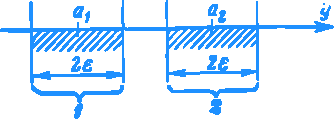
\includegraphics[width=0.55\textwidth,angle=-1]{figures/fig-09.pdf}
\caption{Proving the uniqueness of the limit.}
\label{fig-09}
\end{figure}
This proof contains at least two rather ``delicate'' points. Can you identify them?

\rdr I certainly notice one of them. If $a_{1}$ and $a_{2}$ are limits, no matter how the sequence behaves \emph{at the beginning}, its terms in the long run have to concentrate \emph{simultaneously} around $a_{1}$ and $a_{2}$ which is, of course, impossible

\athr Correct. But there is one more ``delicate'' point, namely, no matter how close $a_{1}$ and $a_{2}$ are, the; should inevitably be spaced by a segment (a gap) of a small but definitely nonzero length.

\rdr But it is self-evident.

\athr I agree. However, this ``self-evidence'' is connected to one more very fine aspect without which the very calculus could not be developed. As you probably noted, one cannot identify on the real line two neighbouring points. If one point is chosen, it is impossible, in principle, to point out its ``neighbouring'' point. In other words, no matter how carefully you select a pair of points on the real line, it is always possible to find any number of points between the two.

Take, for example, the interval $[0, 1]$. Now, exclude the point 1. You will have a half-open interval $[0, 1|$. Can you identify the largest number over this interval?

\rdr No, it is impossible.

\athr That's right. However, if there were a point neighbouring 1, after the removal of the latter this ``neighbour'' would have become the largest number. I would like to note here that many ``delicate'' points and many ``secrets'' in the calculus theorems are ultimately associated with the impossibility of identifying two neighbouring points on the real line, or of specifying the greatest or least 
number on an open interval of the real line.

But let us get back to the properties of convergent sequences and prove the following theorem:
\begin{mytheo}{Theorem}
1f sequences ($y_{n}$) and ($z_{n}$) are convergent (we denote their limits by $a$ and $b$, respectively), a sequence ($y_{n} + z_{n}$) is convergent too, its limit being $a + b$.
\end{mytheo}

\rdr This theorem is none other than rule \eqref{lim-sum} discussed in the	previous dialogue.

\athr Thats right. Nevertheless, I suggest you try to prove it.	

\rdr If we select an arbitrary $\varepsilon > 0$, then there is a number $N_{1}$ such that for all the terms of the first sequence with $n > N_{1}$ we shall have $| y_{n}- a | < \varepsilon$. In addition, for the same $\varepsilon$ there is $N_{2}$ such that for all the terms of the second sequence with $n > N_{2}$ we shall have $| z_{n}- a | < \varepsilon$. Now we select the greatest among $N_{1}$ and $N_{2}$ (we denote it by $N$), then for all $n > N$ both $| y_{n}- a | < \varepsilon$ and $| z_{n}- a | < \varepsilon$. Well, this is as far as I can go.

\athr Thus, you have established that for an arbitrary $\varepsilon$ there is $N$ such that for all $n > N$ both $| y_{n}- a | < \varepsilon$ and $| z_{n}- a | < \varepsilon$ simultaneously. And what can you say about the modulus $| (y_{n} + z_{n}) - (a +b) |$ (for all $n$)? I remind you that $|A + B | \leqslant |A| + |B|$.

\rdr Let us look at
\begin{align*}%
| (y_{n} + z_{n}) - (a +b) | & = |(y_{n}- a )+(z_{n}- b ) | \\
 & \leqslant [ |y_{n}- a| + |z_{n}- b|] \\
 & < (\varepsilon + \varepsilon ) = 2 \varepsilon 
\end{align*}

\athr You have proved the theorem, haven't you?

\rdr But we have only established that there is $N$ such that for all $n>N$ we have $|(y_{n} + z_{n})- (a+b)|< 2\varepsilon$. But we need to prove that
\begin{equation*}%
|(y_{n}+z_{n}) - (a+b) | < \varepsilon 
\end{equation*}
\athr Ah, that's peanuts, if you forgive the expression. In the case of the sequence $(y_{n} + z_{n})$ you select a value of $\varepsilon$, but for the sequences ($y_{n}$) and ($z_{n}$) you must select a e value of $\dfrac{\varepsilon}{2}$ and namely for this value find $N_{1}$ and $N_{2}$.

Thus, we have proved that if the sequences ($y_{n}$) and ($z_{n}$) are convergent, the sequence ($y_{n} + z_{n}$) is convergent too. We have even found a limit of the sum. And do you think that the converse is equally valid?

\rdr I believe it should be. 

\athr You are wrong. Here is a simple illustration:
\begin{align*}
(y_{n}) & =\frac{1}{2}, \,\frac{2}{3}, \,\frac{1}{4}, \,\frac{4}{5}, \,\frac{1}{6}, \,\frac{6}{7}, \,\frac{1}{8}, \, \ldots \\
(z_{n}) & =\frac{1}{2}, \,\frac{1}{3}, \,\frac{3}{4}, \,\frac{1}{5}, \,\frac{5}{6}, \,\frac{1}{7}, \,\frac{7}{8}, \, \ldots \\
(y_{n} + z_{n}) &= 1, \, 1,  \, 1, \, 1, \, 1, \, 1, \, 1, \ldots 
\end{align*}
As you see, the sequences $(y_{n})$ and $(z_{n})$ are not convergent, while the sequence $(y_{n}+ z_{n})$ is convergent, its limit being equal to unity.

Thus, if a sequence $(y_{n}+ z_{n})$ is convergent, two alternatives are possible:
\begin{enumerate}[label=$\textcolor{IndianRed}{\blacktriangleright}$]
\item sequences $(y_{n})$ and $(z_{n})$ are convergent as well, or 
\item sequences $(y_{n})$ and $(z_{n})$ are divergent. 
\end{enumerate}
\rdr But can it be that the sequence  $(y_{n})$ is convergent, while the sequence  $(z_{n})$ is divergent? 

\athr It may be easily shown that this is Impossible.

To begin with, let us note that if the sequence $(y_{n})$ has a limit $a$, the sequence $-(y_{n})$ is also convergent and its limit is $-a$. This follows from an easily proved equality
\begin{equation*}%
\lim\limits_{n \to \infty} (c \, y_{n}) = c \lim\limits_{n \to \infty}  y_{n}
\end{equation*}
where $c$ is a constant. Assume now that a sequence $(y_{n}+ z_{n})$ is convergent to $A$, and that $(y_{n})$ is also convergent and its limit is $a$. Let us apply the theorem on the sum of convergent sequences to the sequences $(y_{n}+ z_{n})$ and $-(y_{n})$. As a result, we obtain that the sequence  $(y_{n}+ z_{n}) - (y_{n})$, i.e. $(z_{n})$, is also convergent, with the limit $A-a$.

\rdr Indeed $(z_{n})$ cannot be divergent in this case.

\athr Very well. Let us discuss now one important particular case of convergent sequences, namely, the so-called \emph{infinitesimal sequence}, or simply, \emph{infinitesimal}. This is the name which is given to a convergent sequence with a limit equal to zero. Sequences \eqref{series-07} and \eqref{series-09} from \hyperref[infinite-seq]{Dialogue One} are examples of infinitesimals.

Note that to any convergent sequence $(y_{n})$ with a limit a there corresponds an infinitesimal sequence ($\alpha_{n}$), where $\alpha_{n} = y_{n} - a$. That is why mathematical analysis is also called calculus of infinitesimals.

Now I invite you to prove the following theorem: 
\begin{mytheo}{Theorem}
If $(y_{n})$ is a bounded sequence and ($\alpha_{n}$) is infinitesimal, then $(y_{n}\alpha_{n}$) is infinitesimal as well.
\end{mytheo}
\rdr Let us select an arbitrary  $\varepsilon > 0$. We must prove that there is $N$ such that for all $n > N$ the terms of the sequence $(y_{n}\alpha_{n}$) satisfy the inequality $|y_{n}\, \alpha_{n}| < \varepsilon$).

\athr Do you mind a hint? As the sequence $(y_{n})$ is bounded, one can find $M$ such that $| y_{n}| \leqslant M$ for any $n$.

\rdr Now all becomes very simple. We know that the sequence  ($\alpha_{n}$) is infinitesimal. It means that for any $\varepsilon' > 0$ we can find $N$ such that for all $n > N |\alpha_{n} | < \varepsilon'$. For $\varepsilon'$, I select $\dfrac{\varepsilon}{M}$ Then, for $n > N$ we have
\begin{equation*}%
|y_{n}\, \alpha_{n}| = |y_{n}| \, |\alpha_{n}|  \leqslant M |\alpha_{n}| < M \frac{\varepsilon}{M}  = \varepsilon
\end{equation*}
This completes the proof. 

\athr Excellent. Now, making use of this theorem, it is very easy to prove another theorem: 
\begin{mytheo}{Theorem}
A sequence ($y_{n}\, z_{n}$) is convergent to $ab$ if sequences ($y_{n}$) and
($z_{n}$) are convergent to $a$ and $b$, respectively.
\end{mytheo}
Suppose $y_{n} = a + \alpha_{n}$ and $z_{n} = b + \beta_{n}$. Suppose also
that the sequences ($\alpha_{n}$) and ($\beta_{n}$) are infinitesimal. Then we
can write:
\begin{equation*}%
y_{n}\, z_{n} = ab + \gamma_{n} \,\, \text{where} \,\, \gamma_{n} = b \alpha_{n} + a \beta_{n} + \alpha_{n} \beta_{n}
\end{equation*}
Making use of the theorem we have just proved, we conclude that the sequences $(b \alpha_{n}), \, (a \beta_{n}) \,\, \text{and} \,\, (\alpha_{n} \beta_{n}) $ are infinitesimal.

\rdr But what justifies your conclusion about the sequence $(\alpha_{n} \beta_{n}) $? 

\athr Because any convergent sequence (regardless of whether it is infinitesimal or not) is bounded. From the theorem on the sum of convergent sequences we infer that the sequence $(y_{n})$ is infinitesimal, which immediately yields
\begin{equation*}%
\lim\limits_{n \to \infty} (y_{n} \,z_{n}) = ab
\end{equation*}
This completes the proof. 

\rdr Perhaps we should also analyze inverse variants in which the sequence $ (y_{n} \,z_{n})$ is convergent. What can be said in this case about the sequences $(y_{n})$ and $(z_{n})$?

\athr Nothing definite. in the general case. Obviously, one possibility is that $(y_{n})$ and $(z_{n})$ are convergent. However, it is also possible, for example, for the sequence $(y_{n})$ to be convergent, while the sequence $(z_{n})$ is divergent. Here is a simple illustration:
\begin{align*}%
(y_{n}) & = 1, \, \frac{1}{4}, \, \frac{1}{9}, \, \frac{1}{16}, \, \frac{1}{25}, \, \ldots \frac{1}{n^{2}}, \, \ldots \\
(z_{n}) & =  1, \, 2, \, 3, \, 4, \, 5, \, \ldots, \, n, \, \ldots \\
(y_{n} \, z_{n}) & =   1, \, \frac{1}{2}, \, \frac{1}{3}, \, \frac{1}{4}, \, \frac{1}{5}, \, \ldots \frac{1}{n}, \, \ldots
\end{align*}
By the way, note that here we obtain an infinitesimal sequence by multiplying an infinitesimal sequence by an unbounded sequence. In the general case, however, such multiplication needn't produce an infinitesimal.

Finally, there is a possibility when the sequence $(y_{n} \, z_{n})$ is convergent, and the sequences $(y_{n})$ and $(z_{n})$ are divergent. Here is one example:
\begin{align*}%
(y_{n}) & = 1, \, \frac{1}{4}, \, 3, \, \frac{1}{16}, \, 5, \, \ldots \frac{1}{36}, \, 7, \, \ldots \\
(z_{n}) & =  1, \, 2, \, \frac{1}{9}, \, 4, \, \frac{1}{25}, \, 6, \, \frac{1}{49}, \, \ldots \\
(y_{n} \, z_{n}) & =   1, \, \frac{1}{2}, \, \frac{1}{3}, \, \frac{1}{4}, \, \frac{1}{5}, \, \frac{1}{6}, \, \frac{1}{7}, \, \ldots
\end{align*}
Now, let us formulate one more theorem: 
\begin{mytheo}{Theorem}
If $(y_{n})$ and $(z_{n})$ are sequences convergent to $a$ and $b$
when $b \neq 0$, then a sequence $\left(\dfrac{y_{n}}{z_{n}}\right)$ is also convergent, its its limit being $\dfrac{a}{b}$.
\end{mytheo}
We shall omit the proof of this theorem,

\rdr And what if the sequence $(z_{n})$ contains zero terms?

\athr Such terms are possible. Nevertheless, the number of such terms can be only finite. Do you know why? 

\rdr I think, I can guess. The sequence $(z_{n})$ has a non-zero limit $b$. 

\athr Let us specify $b > 0$.

\rdr Well, I select $\varepsilon = \dfrac{b}{2}$. There must be an integer $N$ such that $|z_{n} - b | < \dfrac{b}{2}$ for all $n > N$. Obviously all $z_{n}$ (the whole infinite ``tail'' of the sequence) will be positive. Consequently, the zero terms of the sequence $(z_{n})$ may only be encountered among a \emph{finite} number of the first $N$ terms. 

\athr Excellent. Thus, the number of zeros among the terms of $(z_{n})$ can only be finite. If such is the case, one can surely drop these terms. Indeed, \emph{an elimination of any finite number of terms of a sequence does not affect its properties}. For example, a convergent sequence still remains convergent, with its limit unaltered. An elimination of a finite number of terms may only change $N$ (for a given $\varepsilon$), which is certainly unimportant.

\rdr It is quite evident to me that by \emph{eliminating} a finite number of terms one does not affect the convergence of a sequence. But could an \emph{addition} of a finite number of terms affect the convergence of a sequence?

\athr A finite number of new terms does not affect the convergence of a sequence either. No matter how many new terms are added and what their new serial numbers are, one can always find the greatest number $N$ after which the whole infinite ``tail'' of the sequence is unchanged. No matter how large the number of new terms may be and where you insert them, the finite set of new terms cannot change the infinite ``tail'' of the sequence. And it is the ``tail'' that determines the convergence (divergence) of a sequence.

Thus, we have arrived at the following: 
\begin{mytheo}{Conclusion}
Elimination, addition, and any other change of a finite number of terms of a sequence do not affect either its convergence or its limit (if the sequence is convergent).
\end{mytheo}

\rdr I guess that an elimination of an infinite number of terms (for example, every other term) must not affect the convergence of a sequence either.

\athr Here you must be very careful. If an initial sequence is convergent, an elimination of an infinite number of its terms (provided that the number of the remaining terms is also infinite) does not affect either convergence or the limit of the sequence. If, however, an initial sequence is divergent, an elimination of an infinite number of its terms may, in certain cases, convert the sequence into a convergent one. For example, if you eliminate from divergent sequence \eqref{series-10} (see \hyperref[infinite-seq]{Dialogue One}) all the terms with even serial numbers, you will get the convergent sequence.
\begin{equation*}%
1, \, \frac{1}{3}, \, \frac{1}{5}, \,\frac{1}{7}, \,\frac{1}{9}, \,\frac{1}{11}, \,\frac{1}{13}, \, \ldots
\end{equation*}
Suppose we form from a given convergent sequence two new convergent sequences. The first new sequence will consist of the terms of the initial sequence with \emph{odd} serial numbers, while the second will consists of the terms with \emph{even} serial numbers. What do you think are the limits of these new sequences?

\rdr It is easy to prove that the new sequences will have the same limit as the initial sequence.

\athr You are right. 

Note that from a given convergent sequence we can form not only two but a \emph{finite number} $m$ of new sequences converging to the same limit. One way to do it is as follows. The first	new sequence will consist of the 1st, $(m + 1)$st, $(2m + 1)$st, $(3m + 1)$st, etc., terms of the initial sequence. The second	sequence will consist of the 2nd, $(m + 2)$nd, $(2m + 2)$nd, $(3m + 2)$nd, etc., terms of the initial sequence.

Similarly we can form the third, the fourth, and other sequences.

In conclusion, let us see how one can ``spoil'' a convergent sequence by turning it into divergent. Clearly, different ``spoiling'' approaches are possible. Try to suggest something simple.

\rdr For example, we can replace all the terms with even serial numbers by a constant that is not equal to the limit of the initial sequence. For example, convergent sequence \eqref{series-05} (see \hyperref[infinite-seq]{Dialogue One})  can be ``spoilt'' in the following manner:
\begin{equation*}%
\frac{1}{2}, \, 2, \, \frac{3}{4}, \, 2, \, \frac{5}{6}, \, 2, \, \frac{7}{8}, \, 2,  \, \ldots
\end{equation*}

\athr I see that you have mastered very well the essence of the concept of a convergent sequence. Now we are ready for another substantial step, namely, consider one of the most important concepts in calculus: the definition of a function.
}
% !TEX root = calculus.tex

\chapter{FUNCTION}
\label{function}
{\parindent=0pt

\rdr Functions are widely used in elementary mathematics.

\athr Yes, of course. You are familiar with \emph{numerical functions}. Moreover, you have worked already with different numerical functions. Nevertheless, it will be worthwhile to dwell on the concept of the function. To begin with, what is your idea of a function?

\rdr As I understand it, a function is a certain correspondence between \emph{two variables}, for example, between $x$ and $y$. Or rather, it is a dependence of a variable $y$ on a variable $x$.

\athr What do you mean by a ``variable''?

\rdr It is a quantity which may assume different values.

\athr Can you explain what your understanding of the expression ``a quantity assumes a value'' is? What does it mean? And what are the reasons, in particular, that make a quantity to assume this or that value? Don't you feel that the very concept of a variable quantity (if you are going to use this concept) needs a definition?

\rdr O.K., what if I say: a function $y = f (x)$ symbolizes a dependence of $y$ on $x$, where $x$ and $y$ are numbers.

\athr I see that you decided to avoid referring to the concept of a \emph{variable quantity}. Assume that $x$ is a number and $y$ is also a number. But then explain, please, the meaning of the phrase ``a dependence between two numbers''.

\rdr But look, the words ``an independent variable'' and ``a dependent variable'' can be found in any textbook on mathematics.

\athr The concept of a variable is given in textbooks on mathematics after the definition of a function has been introduced.

\rdr It seems I have lost my way.

\athr Actually it is not all that difficult ``to construct'' an image of a numerical function. I mean \emph{image}, not \emph{mathematical definition} which we shall discuss later.

In fact, a numerical function may be pictured as a ``black box'' that \emph{generates a number at the output in response to a number at the input}. You put into this ``black box'' a number (shown by $x$ in \hyperref[fig-10]{Figure \ref{fig-10}}) and the "black box" outputs a new number ($y$ in \hyperref[fig-10]{Figure \ref{fig-10}}).
\begin{figure}[!h]
\centering
\begin{tikzpicture}[line cap=round,line join=round,>=triangle 45,x=0.5cm,y=.6cm]
\clip(-8,-3) rectangle (7,4);
\fill[line width=2.pt,color=DimGray,fill=DarkGray,fill opacity=0.25,rounded corners=8pt] (3.,2.) -- (-3.,2.) -- (-3.,-1.) -- (3.,-1.) -- cycle;
\filldraw[DimGray] (2.5,1.75) -- (-2.5,1.75) -- (-2.5,1.1) -- (2.5,1.1) -- cycle;

\draw [line width=.75pt,color=IndianRed] (6.,3.) circle (12pt);
\draw [line width=.75pt,color=IndianRed] (6.,3.) circle (8pt);
%\draw [line width=1.2pt,color=DarkGray] (3.,2.)-- (-3.,2.);
%\draw [line width=1.2pt,color=DarkGray] (-3.,-1.)-- (3.,-1.);
%\draw [line width=1.2pt,color=DarkGray] (-3.,-1.)-- (-3,2.);
%\draw [line width=1.2pt,color=DarkGray] (3.,-1.)-- (3.,2.);
\draw [line width=.75pt,color=IndianRed] (-6.,-2.) circle (12pt);
\draw [line width=.75pt,color=IndianRed] (-6.,-2.) circle (8pt);
\draw (-.1,0.7)node[color=black] {\footnotesize \textit{``Black Box''}};
\draw (-0.1,0.)node[color=black] {\footnotesize Working as a };
\draw (0.,-0.6)node[color=black] {\footnotesize Function};
\draw (6,3) node[color=black] {$x$};
\draw (6,2.4) node[color=black](one) {};
\draw (-6,-2) node[color=black] {$y$};
\draw (-5.4,-2) node[color=black] (two) {};
\draw (0,1.85) node[color=black](onea){};
\draw (0,-.9) node[color=black](twoa){};
\path (one) edge[-{latex},line width=2.5pt,in=90,out=270,color=DodgerBlue] (onea);
\path (twoa) edge[-{latex},line width=2.5pt,in=0,out=270,color=DodgerBlue] (two);
\end{tikzpicture}
%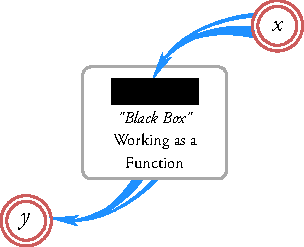
\includegraphics[width=0.55\textwidth]{figures/fig-10.pdf}
\caption{A numerical function as a black box.}
\label{fig-10}
\end{figure}
Consider, for example, the following function: 
\begin{equation*}%
y = 4x^{2} - 1
\end{equation*}
If the input is $x= 2$, the output is $y=15$; if the input is $x=3$, the output is $y= 35$; if the input is $x=10$, the output is $y = 399$, etc.

\rdr What does this ``black box'' look like? You have stressed that \hyperref[fig-10]{Figure \ref{fig-10}} is only symbolic.

\athr In this particular case it makes no difference. It does not influence the essence of the concept of a function. But a function can also be ``pictured'' like this:
\begin{equation*}%
4 \Box^{2} - 1
\end{equation*}
The square in this picture is a ``window'' where you input the numbers. Note that there may be more than one ``window''. For example,
\begin{equation*}%
\frac{4 \Box^{2} - 1}{|\Box| + 1}
\end{equation*}

\rdr Obviously, the function you have in mind is 
\begin{equation*}%
\frac{4 x^{2} - 1}{|x| + 1}
\end{equation*}

\athr Sure. In this case each specific value should be input into both ``windows'' simultaneously. ``Black box'' working as a function
 \hyperref[fig-10]{Figure \ref{fig-10}}.

By the way, it is always important to see such a ``window'' (or ``windows'') in a formula describing the function. Assume, for example, that one needs to pass from a function $y = f (x)$ to a function $y = f(x - 1)$ (on a graph of a function this transition corresponds to a displacement of the curve in the positive direction of the $x$-axis by 1). If you clearly understand the role of such a ``window'' (``windows''), you will simply replace in this ``window'' (these ``windows'') $x$ by $x - 1$. Such an operation is Illustrated by \hyperref[fig-11]{Figure \ref{fig-11}} which represents the following function
\begin{equation*}%
y = \frac{4 x^{2} - 1}{|x| + 1}
\end{equation*}
\begin{figure}[!h]
\centering
\begin{tikzpicture}[line cap=round,line join=round,>=triangle 45,rounded corners,x=1cm,y=1cm]
%\clip(-8,-3) rectangle (7,4);
  \draw (-3,2) [color=IndianRed]rectangle (-1,0) node[pos=.5,align=center,] {$\dfrac{4x^{2}-1}{|x|+ 1} $};
  \draw (-1.5,1.5) [color=black]rectangle (2,4) node[pos=.5,align=center] {\Large$\dfrac{4 \Box^{2}-1}{|\Box|+ 1} $};
  \draw (3.5,1.75) [color=IndianRed] rectangle (6.5,3.75) node[pos=.5,align=center] { $\dfrac{4(x-1)^{2}-1}{|x-1|+ 1} $};
  \draw (1,4.25) [color=DodgerBlue]rectangle (3,5) node[pos=.5,align=center]{ $|x-1| $};
  \draw (1,.5) [color=DodgerBlue]rectangle (3,1.25) node[pos=.5,align=center] { $|x-1| $};
\draw (1.1,4.65) node[color=black](onea) {};
\draw (1.1,.85) node[color=black](twoa) {};  
\draw (-0.2,3.2) node[color=black](one) {};
\draw (-.2,2.35) node[color=black] (two) {};
\draw (3.65,2.75) node[color=black](three) {};
\draw (1.9,2.75) node[color=black] (threea) {};
\path (one) edge[{latex}-,line width=2.5pt,in=180,out=90,color=DodgerBlue] (onea);
\path (twoa) edge[-{latex},line width=2.5pt,in=270,out=180,color=DodgerBlue] (two);
\path (three) edge[{latex}-,line width=3.5pt,in=0,out=180,color=DodgerBlue] (threea);
\end{tikzpicture}
%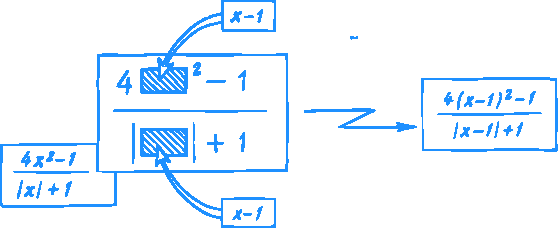
\includegraphics[width=0.9\textwidth]{figures/fig-11.pdf}
\caption{Change in a function from $f(x) \to f(x-1)$.}
\label{fig-11}
\end{figure}
Obviously, as a result of substitution of $x - 1$ for $x$ we arrive at a new function (new ``black box'') 
\begin{equation*}%
\frac{4 (\Box - 1)^{2} - 1}{|\Box -1 | + 1}, \quad y = \frac{4 (x - 1)^{2} - 1}{|x -1 | + 1}
\end{equation*}

\rdr I see. If, for example, we wanted to pass from $y = f (x)$ to $y = f \left( \frac{1}{x} \right)$, the function pictured in \fig{fig-11} would be transformed as follows:
\begin{equation*}%
y = \frac{\dfrac{4}{x^{2}} -1 }{\dfrac{1}{|x |} + 1}
\end{equation*}

\athr Correct. Now. try to find $y = f (x)$ if
\begin{equation*}%
2 f	\left( \dfrac{1}{x } \right) - f(x) = 3x
\end{equation*}

\rdr I am at a loss. 

\athr As a hint, I suggest replacing $x$ by $\dfrac{1}{x } $.

\rdr This yields
\begin{equation*}%
2 f (x)	- f \left( \dfrac{1}{x } \right) = \frac{3}{x}
\end{equation*}
Now it is clear. Together with the initial equation, the new equation forms a system of two equations for $f (x)$ and $f \left( \dfrac{1}{x } \right) $:
\begin{equation*}
\left.
\begin{split}
2f \left( \dfrac{1}{x } \right) - f(x) & = 3x \\
2 f(x) - f \left( \dfrac{1}{x } \right)  & = \frac{3}{x}
\end{split}
\right\}
\end{equation*}

By multiplying all the terms of the second equation by 2 and then adding them to the first equation, we obtain
\begin{equation*}%
 f (x) = x + \frac{2}{x}
\end{equation*}


\athr Perfectly true.

\rdr In connection with your comment about the numerical function as a ``black box'' generating a numerical output in response to a numerical input, I would like to ask whether other types of ``black boxes'' are possible in calculus. 

\begin{figure}[!h]
\centering
\begin{tikzpicture}[line cap=round,line join=round,>=triangle 45,rounded corners,x=1cm,y=1cm,scale=1]
%  \draw[step=.5cm,gray,very thin] (-5,-5) grid (5,5);

\clip(-7.1,-.1) rectangle (5.1,5.1);
\draw (-4,4) [color=IndianRed]rectangle (-2,5) node[pos=.5,align=center]{\small number};
\draw (-.5,4) [color=IndianRed]rectangle (1.5,5) node[pos=.5,align=center]{\small {numerical} \\[-5pt] \small{ function}};
\draw (3,4) [color=IndianRed]rectangle (5,5) node[pos=.5,align=center]{\small {numerical} \\[-5pt] \small{ function}};

  \draw (-5.5,2) [color=IndianRed]rectangle (-3.5,3) node[pos=.5,align=center] {\small {numerical} \\[-5pt] \small{ function}};    
  \draw (-2,2) [color=IndianRed]rectangle (0,3) node[pos=.5,align=center] {\small operator};  
  \draw (1.5,2) [color=IndianRed]rectangle (3.5,3) node[pos=.5,align=center] {\small functional};

        \draw (-7,0) [color=IndianRed]rectangle (-5,1) node[pos=.5,align=center] {\small  number};    
    \draw (-3.5,0) [color=IndianRed]rectangle (-1.5,1) node[pos=.5,align=center] {\small {numerical} \\[-5pt] \small{ function}};
 \draw (0,0) [color=IndianRed]rectangle (2,1) node[pos=.5,align=center] {\small number};

\draw (4,4.1) node[color=black](1a) {};
\draw (2.5,2.8) node[color=black](1b) {};
\draw (2.5,2.1) node[color=black](1c) {};
\draw (1,.8) node[color=black](1d) {};

\draw (0.5,4.1) node[color=black](2a) {};
\draw (-1,2.8) node[color=black](2b) {};
\draw (-1,2.1) node[color=black](2c) {};
\draw (-2.5,.8) node[color=black](2d) {};

\draw (-3,4.1) node[color=black](3a) {};
\draw (-4.5,2.8) node[color=black](3b) {};
\draw (-4.5,2.1) node[color=black](3c) {};
\draw (-6,.8) node[color=black](3d) {};

\path (1a) edge[-{latex},line width=1.5pt,in=90,out=270,color=DodgerBlue] (1b);
\path (1c) edge[-{latex},line width=1.5pt,in=90,out=270,color=DodgerBlue] (1d);

\path (2a) edge[-{latex},line width=1.5pt,in=90,out=270,color=DodgerBlue] (2b);
\path (2c) edge[-{latex},line width=1.5pt,in=90,out=270,color=DodgerBlue] (2d);

\path (3a) edge[-{latex},line width=1.5pt,in=90,out=270,color=DodgerBlue] (3b);
\path (3c) edge[-{latex},line width=1.5pt,in=90,out=270,color=DodgerBlue] (3d);

\end{tikzpicture}
%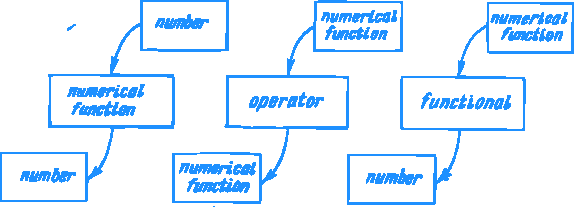
\includegraphics[width=\textwidth]{figures/fig-12.pdf}
\caption{Understanding place and role of the numerical function as a mathematical tool.}
\label{fig-12}
\end{figure}

\athr Yes, they are. In addition to the numerical function, we shall discuss the concepts of an operator and a functional. 

\rdr I must confess I have never heard of such concepts. 

\athr I can imagine. I think, however, that \fig{fig-12} will be helpful. Besides, it will elucidate the place and role of the numerical function as a mathematical tool. \fig{fig-12} shows that:
\begin{enumerate}[label=$\textcolor{IndianRed}{\blacktriangleright}$]

\item \emph{a numerical function is a \emph{``black box''} that generates a number at the output in response to a number at the input;}

\item \emph{an operator	is	a \emph{``black box''} that	generates	a	numerical function at the output in response to a numerical function at the input}; it is said that all operator applied to a function generates a new function;

\item \emph{a functional is a \emph{``black box''} that generates a number at the output in response to a numerical junction at the input}, i.e. a concrete number is obtained ``in response'' to a concrete function.
\end{enumerate}

\rdr Could you give examples of operators and functionals?

\athr Wait a minute. In the next dialogues we shall analyze both the concepts of an operator and a functional. So far, we shall confine ourselves to a general analysis of both concepts. Now we get back to our main object, the numerical function.

The question is: How to construct a ``black box'' that generates a numerical function.

\rdr Well, obviously, we should find a relationship, or a law, according to which the number at the ``output'' of the ``black box'' could be forecast for each specific number introduced at the ``input''.

\athr You have put it quite clearly. Note that such a law could be naturally referred to as the \emph{law of numerical correspondence}. However, the law of numerical correspondence would not be a sufficient definition of a numerical function.

\rdr What else do we need?

\athr Do you think that any number could be fed into a specific ``black box'' (function)?

\rdr I see. I have to define a set of numbers acceptable as inputs of the given function.

\athr That's right. This set is said to be the \emph{domain of a function}.

Thus, the definition of a numerical function is based on two ``cornerstones'';

the domain of a function (a certain set of numbers), and the law of numerical correspondence. 

According to this law, \emph{every number from the domain of
a function is placed in correspondence with a certain number, which is called the value of the function; the values form the range of the function.}

\rdr Thus, we actually have to deal with two numerical sets. On the one hand, we have a set called the domain of a function and, on  the other, we have a set called the range of a function.

\athr At this juncture we have come closest to a mathematical definition of a function which will enable us to avoid the somewhat mysterious word ``black box''.

Look at \fig{fig-13}. It shows the function $y = \sqrt{1 - x^{2}}$.  \fig{fig-13} pictures two numerical sets, namely, $D$ (represented by the interval $[-1, 1]$) and	 $E$ (the interval $[0, 1]$). For your convenience these sets are shown on two different real lines.

\begin{figure}[!h]
\centering
\begin{tikzpicture}[line cap=round,line join=round,>=triangle 45,rounded corners,scale=1.5]
\clip(-2.2,-1.1) rectangle (4.5,5);
% \draw[step=.5cm,gray,very thin] (-3,-3) grid (6,6);
{\footnotesize
\draw (0,0) node[color=black,below](0a){0};
\draw (0,-.75) node[color=black,below]{D};
\draw (-2,0) node[color=black,below](-2a) {-1};
\draw (2,0) node[color=black,below](2a) {1};
\draw (-1.5,0) node[color=black,below](-15a) {};
\draw (1.5,0) node[color=black,below](15a) {};
\draw (-1,0) node[color=black,below](-1a) {};
\draw (1,0) node[color=black,below](1a) {};
\draw (-.5,0) node[color=black,below](-5a) {};
\draw (.5,0) node[color=black,below](5a) {};

\draw (3.5,1.5) node[color=black,right](0b){0};
\draw (4.2,2.7) node[color=black,right]{E};
\draw (3.5,4) node[color=black,right](2b) {1};
\draw (3.5,3.90) node[color=black,right](3b) {};% {0.96};
\draw (3.5,3.65) node[color=black,right](4b){};% {0.86};
\draw (3.5,3.15) node[color=black,right](5b){};% {0.66};


\draw [->,line width=1.2pt,color=DarkGray] (-2.5,0.) -- (3.5,0.);
\draw [->,line width=1.2pt,color=DarkGray] (3.5,1.) -- (3.5,5.);

\path (0a) edge[-{latex},line width=1.5pt,in=180,out=90,color=DodgerBlue] (2b);

\path (2a) edge[-{latex},line width=1.5pt,in=180,out=90,color=DodgerBlue] (0b);
\path (-2a) edge[-{latex},line width=1.5pt,in=180,out=90,color=DodgerBlue,looseness=.8] (0b);


\path (15a) edge[-{latex},line width=1.5pt,in=180,out=90,color=DodgerBlue] (5b);
\path (-15a) edge[-{latex},line width=1.5pt,in=180,out=90,color=DodgerBlue,looseness=.8] (5b);

\path (1a) edge[-{latex},line width=1.5pt,in=180,out=90,color=DodgerBlue] (4b);
\path (-1a) edge[-{latex},line width=1.5pt,in=180,out=90,color=DodgerBlue,looseness=.8] (4b);

\path (5a) edge[-{latex},line width=1.5pt,in=180,out=90,color=DodgerBlue] (3b);
\path (-5a) edge[-{latex},line width=1.5pt,in=180,out=90,color=DodgerBlue,looseness=.8] (3b);

\draw [decoration={brace,amplitude=20pt},decorate,rotate=-90,color=DarkGray,line width=.5pt] ($(2a)+(0.25em,.5ex)$) -- ($(-2a)+(0.25em,-.5ex)$);

\draw [decoration={brace,amplitude=20pt},decorate,rotate=-90,color=DarkGray,line width=.5pt] ($(2b)+(0.25em,.5ex)$) -- ($(0b)+(0.25em,.5ex)$);
}
\end{tikzpicture}

%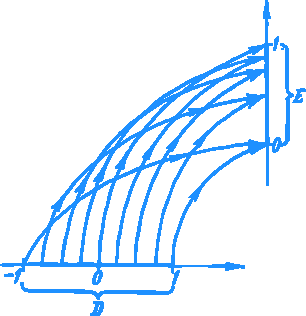
\includegraphics[width=0.55\textwidth]{figures/fig-13.pdf}
\caption{Range and domain of a function.}
\label{fig-13}
\end{figure}

The set $D$ is the domain of the function, and $E$ is its range. Each number in $D$ corresponds to one number in $E$ (every input value is placed in correspondence with one output value). This correspondence is shown in \fig{fig-13} by arrows pointing from $D$ to $E$.


\rdr But \fig{fig-13} shows that two \emph{different} numbers in $D$ correspond to one number in $E$.

\athr It does not contradict the statement ``each number in $D$ corresponds to one number in $E$.'' I never said that \emph{different} numbers in $D$ must correspond to different numbers in $E$. Your remark (which actually stems from specific characteristics of the chosen function) is of no principal significance. Several numbers in $D$ may correspond to one number in $E$. An inverse situation, however, is forbidden. It is not allowed for one number in $D$ to correspond to more than one number in $E$. I emphasize that each number in $D$ must correspond to \emph{only one} (not more!) number in $E$.

Now we can formulate a mathematical definition of the numerical function.

\begin{mytheo}{Definition}
Take two numerical sets $D$ and $E$ in which each element $x$ of $D$ (this is denoted by $x \in D$) is placed in one-to-one correspondence with one element $y$ of $E$. Then we say that a function $y = f (x)$ is set in the domain $D$, the range of the function being $E$. It is said that the argument $x$ of the function $y$ passes through $D$ and the values of $y$ belong to $E$.
\end{mytheo}

Sometimes it is mentioned (but more often omitted altogether) that both $D$ and $E$ are subsets of the set of real numbers $R$ (by definition, $R$ is the real line).

On the other hand, the definition of the function can be reformulated using the term ``mapping''. Let us return again to \fig{fig-13}. Assume that the number of arrows from the points of $D$ to the points of $E$ is infinite (just imagine that such arrows have been drawn from each point of $D$). Would you agree that such a picture brings about an idea that $D$ is \emph{mapped} onto $E$?

\rdr Really, it looks like mapping.

\athr Indeed, this \emph{mapping} can be used to define the \emph{function}.
\begin{mytheo}{Definition}
A numerical function is a mapping of a numerical set $D$ (which is the domain of the function) onto another numerical set $E$ (the range of this function).
\end{mytheo}
Thus, the numerical function is a \emph{mapping of one numerical set onto another numerical set.} The term ``mapping'' should be understood as a kind of numerical correspondence discussed above. In the notation $y = f (x)$, symbol $f$ means the function itself (i.e. the mapping), with $x \in D$ and $y \in E$.

\rdr If the \emph{numerical function} is a mapping of one numerical set onto another numerical set, then the operator can be considered as a mapping of a set of numerical function onto another set of functions, and the \emph{functional} as a mapping of a set of functions onto a numerical set.

\athr You are quite right.

\rdr I have noticed that you persistently use the term ``numerical function'' (and I follow suit), but usually one simply says ``function''. Just how necessary is the word ``numerical''?

\athr You have touched upon a very important aspect. The point is that in modern mathematics the concept of a function is substantially broader than the concept of a numerical function. As a matter of fact, the concept of a function includes, as particular cases, a numerical function as well as an operator and a functional, because the essence in all the three is a mapping of one set onto another independently of the nature of the sets. You have noticed that both operators and functionals are mappings of certain sets onto certain sets. In a particular case of mapping of a numerical set onto a numerical set we come to a \emph{numerical} function. In a more general case, however, sets to be mapped can be \emph{arbitrary}. Consider a few examples.

\textcolor{IndianRed}{\textbf{Example 1}} Let $D$ be a set of working days in an academic year, and $E$ a set of students in a class. Using these sets, we can define a function realizing a schedule for the students on duty in the classroom. In compiling the schedule, each element of $D$ (every working day in the year) is placed in one-to-one correspondence with a certain element of $E$ (a certain student). This function is a \emph{mapping of the set of working days onto the set of students}. We may add that the domain of the function consists of the working days and the range is defined by the set of the students.

\rdr It sounds a bit strange. Moreover, these sets have finite numbers of elements.

\athr This last feature is not principal.

\rdr The phrase ``the values assumed on the set of students'' sounds somewhat awkward.

\athr Because you are used to interpret ``value'' as ``numerical value''.
Let us consider some other examples.

\textcolor{IndianRed}{\textbf{Example 2}} Let $D$ be a set of all triangles, and $E$ a set of positive real numbers. Using these sets, we can define two functions, namely, the area of a triangle and the perimeter of a triangle. Both functions are mappings (certainly, of different nature) \emph{of the set of the triangles onto the set of the positive real numbers}. It is said that the set of all the triangles is the domain of these functions and the set of the positive real numbers is the range of these functions.

\textcolor{IndianRed}{\textbf{Example 3}} Let $D$ be a set of all triangles, and $E$ a set of all circles. The mapping of $D$ onto $E$ can be either a circle inscribed in a triangle, or a circle circumscribed around a triangle. Both have the set of all the triangles as the domain of the function and the set of all the circles as the range of the function.

By the way, do you think that it is possible to ``construct'' an \emph{inverse} function in a similar way, namely, to define a function with all the circles as its domain and all the triangles as its range?

\rdr I see no objections.

\athr No, it is impossible. Because any number of different triangles can be inscribed in or circumscribed around a circle. In other words, each element of $E$ (each circle) corresponds to an Infinite number of different elements of $D$ (i.e, an infinite number of triangles). It means that there is no function since no mapping can be realized.

However, the situation can be improved if we restrict the set of triangles.

\rdr I guess I know how to do it. We must choose the set of all the \emph{equilateral} triangles as the set $D$. Then it becomes possible to realize both a mapping of $D$ onto $E$ (onto the set of all the circles) and an inverse mapping, i.e. the mapping of $E$ onto $D$, since only one equilateral triangle could be inscribed in or circumscribed around a given circle.

\athr Very good. I see that, you have grasped the essence of the concept of functional relationship. I should emphasize that from the broadest point of view this concept is based on the idea of mapping one set of objects onto another set of objects. \emph{It means that a function can be realized as a numerical function, an operator, or a functional}. As we have established above, a \emph{function may be represented by an area or perimeter of a geometrical figure, such, as a circle inscribed in a triangle or circumscribed around it, or it may take the form of a schedule of students on duty in a classroom, etc}. It is obvious that a list of different functions may be unlimited.

\rdr I must admit that such a broad interpretation of the concept of a function is very new to me.

\athr As a matter of fact, in a very diverse set of possible functions (mappings), we shall use only \emph{numerical functions, operators}, and \emph{functionals}. Consequently, we shall refer to numerical functions as simply \emph{functions}, while \emph{operators} and \emph{functionals} will be pointed out specifically.

And now we shall examine the already familiar concept of a numerical sequence as an example of mapping.

\rdr A numerical sequence is, apparently, a mapping of a set of natural numbers onto a different numerical set. The elements of the second set are the terms of the sequence. Hence, a numerical sequence is a particular case of a numerical function. The domain of a function is represented by a set of natural numbers.

\athr This is correct. But you should bear in mind that later on we shall deal with numerical functions whose domain is represented by the \emph{real line}, or by its \emph{interval} (or \emph{intervals}), and whenever we mention a function, we shall imply a numerical function.

In this connection it is worthwhile to remind you of the classification of intervals. In the previous dialogue we have already used this classification, if only partially.

First of all we should distinguish between the intervals of finite length:
\begin{enumerate}[label=$\textcolor{IndianRed}{\blacktriangleright}$]

\item a \emph{closed interval} that begins at $a$ and ends at $b$ is denoted by $[a, b]$; the numbers $x$ composing this interval meet the inequalities $a \leqslant x \leqslant b$;

\item an \emph{open interval} that begins at $a$ and ends at $b$ is denoted by $]\, a, b[$; the numbers $x$ composing this interval meet the inequalities	$a < x < b$;

\item a \emph{half-open interval} is denoted either by $] \, a, b]$ or $[a, b[$, the former implies that $ a < x \leqslant b$, and the latter that $a \leqslant x < b$.
\end{enumerate}

The intervals may also be \emph{infinite}:
\begin{center}
\begin{tabular}{llc}
$]\, - \infty, \, \infty \, [$ &	$( -	\infty < x < \infty)$ &	the real line \\
$] \, a, \, \infty  \, ]$ & $(a < x < \infty)$ & \\
$[\, a, \, \infty \, [$ &  $(a  \leqslant x < \infty)$ & \\
$] \, - \infty, b \, [$ & $(- \infty < x < b)$ & \\
$ ]- \infty, \, b]$  & $(-  \infty < x \leqslant b)$ & \\
\end{tabular}
\end{center}

Let us consider several specific examples of numerical functions. Judging by the appearance of the formulas given below, point out the intervals constituting the domains of the following functions:
\begin{align}%
y & = \sqrt{ 1 - x^{2}}	\label{fn-ex-01}\\
%eq(1) 
y & = \sqrt{ x - 1}		\label{fn-ex-02}\\
%eq(2) 
y & = \sqrt{2 - x} 	\label{fn-ex-03}\\
%eq(3)
y & = \dfrac{1}{\sqrt{x-1}}	\label{fn-ex-04}\\	
%eq(4)
y & = \dfrac{1}{\sqrt{2-x}}		\label{fn-ex-05}\\
%eq(5) 
y & = 	\sqrt{x-1} + \sqrt{2-x}\label{fn-ex-06}\\
%eq(6) 
y & = \dfrac{1}{\sqrt{x-1}}	+ \dfrac{1}{\sqrt{2 -x }}		\label{fn-ex-07}\\
%eq(7)
y & =	\sqrt{2 -x } +  \dfrac{1}{\sqrt{x-1}}	 	\label{fn-ex-08}\\
%eq(8)
y & = \sqrt{x-1} +	\dfrac{1}{\sqrt{2 -x }} \label{fn-ex-09}
%eq(9)
\end{align}
\rdr It is not difficult. The domain of function \eqref{fn-ex-01} is the interval $(-1, \, 1]$; that of \eqref{fn-ex-02} is $[1, \, \infty[$; that of \eqref{fn-ex-03} is $]-\infty, \, 2]$; that of \eqref{fn-ex-04} is $]\, 1, \infty[$; that of \eqref{fn-ex-05} is $]\infty, 2[$; that of \eqref{fn-ex-06} is $[1, 2]$, etc.

\athr Yes, quite right, but may I interrupt you to emphasize that if a function is a sum (a difference, or a product) of two functions, its domain is represented by the \emph{intersection} of the sets which are the domains of the constituent functions. It is well illustrated by function \eqref{fn-ex-06}. As a matter of fact, the same rule must be applied to functions \eqref{fn-ex-07}-\eqref{fn-ex-09}. Please, continue.

\rdr The domains of the remaining functions are \eqref{fn-ex-07} $]1, 2[$; \eqref{fn-ex-08} $]1,2]$; \eqref{fn-ex-09} $[1, 2[$.

\athr And what can you say about the domain of the function $y= \sqrt{x -2 } + \sqrt{1 -x }$?

\rdr The domain of  $y= \sqrt{x -2 }$ is $[2, \infty[$, while that of  $y= \sqrt{1 -x }$is $]- \infty, 1]$. These intervals do not intersect.

\athr It means	that the formula  $y= \sqrt{x -2 } + \sqrt{1 -x }$ does not define any function.
}
% !TEX root = calculus.tex

\chapter{MORE ON FUNCTION}
\label{more-on-function}
{\parindent=0pt
\athr Let us discuss the methods of defining functions. One of them has already been employed quite extensively. I mean the \emph{analytical description} of a function by some \emph{formula}, that is, an \emph{analytical expression} (for example, expressions \eqref{fn-ex-01} through \eqref{fn-ex-09} examined at the end of the preceding dialogue).

\rdr As a matter of fact, my concept of a function was practically reduced to its representation by a' formula. It was a formula that I had in mind whenever I spoke about a dependence of a variable $y$ on a variable $x$.

\athr Unfortunately, the concept of a function as a formula relating $x$ and $y$ has long been rooted in the minds of students. This is, of course, quite wrong. A function and its formula are very different entities. It is one thing to define a function as a mapping of one set (in our case it is a numerical set) onto another, in other words, as a ``black box'' that generates a number at the output in response to a number at the input. It is quite another thing to have just a formula, which represents only one of the ways of defining a function. It is wrong to \emph{identify} a function with a formula giving its analytical description (unfortunately, it happens sometimes).

\rdr It seems that after the discussion in the previous dialogue about the function, such identification in a general case is automatically invalidated. However, if we confine ourselves only to numerical functions and if we bear in mind that working with a function we always use a formula to describe it, a question arises: Why is it erroneous to identify these two notions? Why should we always emphasize the difference between the function and its formula?

\athr I'll tell you why. First, not every formula defines a function. Actually, at the end of the previous dialogue we already had such an example. I shall give you some more: 
\begin{align*}%
y &= \dfrac{1}{\sqrt{x}} +  \dfrac{1}{\sqrt{-x}}   \\
y &= \log x + \log \, (-x), \\
y & = \sqrt{\sin x - 2}, \\
y & = \log \, (\sin x - 2), \,\, \text{etc.} 
\end{align*}
These formulas do not represent any functions.

Second (and this is more important), not all functions can be written as formulas. One example is the so-called \emph{Dirichlet function} which is defined on the real line:
\begin{equation*}%
y = 
\begin{cases}
 1 & \text{ if $x$ is a rational number} \\
 0 & \text{ if $x$ is an irrational number }
\end{cases}
\end{equation*}
\rdr You call \emph{this} a function?

\athr It is certainly an unusual function, but still a function. It is a mapping of a set of rational numbers to unity and a set of irrational numbers to zero. The fact that you cannot suggest any analytical expression for this function is of no consequence (unless you invent a special symbol for the purpose and look at it as a formula).

However, there is one more, third and probably the most important, reason why functions should not be identified with their formulas. Let us look at the following expression:
\begin{equation*}%
y = 
\begin{cases}
\cos x &  x < 0 \\
1 + x^{2} & 0 \leqslant x \leqslant 2 \\
\log \, (x - 1) & x > 2 
\end{cases}
\end{equation*}
How many functions have I defined here? 

\rdr Three functions: a cosine, a quadratic function, and a logarithmic function. 

\athr You are wrong. The \emph{three formulas} ($y = \cos x, \,\,
y = 1 + x^{2}$, and $y=\log (x- 1)$) define in this case a \emph{single function}. It is defined on the real line, with the law of numerical correspondence given as $y = \cos x$ over the interval $]-\infty, 0 \, [$, as $y = 1 + x^{2}$ over the interval $[0,2]$, and as $y = \log (x - 1)$ over the interval $]2, \infty \,[$.

\rdr I've made a mistake because I did not think enough about the question.

\athr	No, you have made the mistake because subconsciously you identified a function with its analytical expression, i.e. its formula. Later on, operating with functions, we shall use formulas rather extensively. However, you should never forget that a formula is not all a function is, It is only one way of defining it.

The example above illustrates, by the way, that one should not identify such notions as the \emph{domain of a function} and the \emph{range of} $x$ on which an analytical expression is defined (i.e. the domain of an analytical expression). For example, the expression $1 + x^{2}$ is defined on the real line. However, in the example above this expression was used to define the function only over the interval $[0, 2]$.

It should be emphasized that the question about the domain of a function is of principal significance. It goes without saying that the domain of a function cannot be wider than the domain of an analytical expression used to define this
function. But it can be narrower.

\rdr Does it mean that a cosine defined, for example, over the interval $[0, \pi]$ and a cosine defined over the interval $[\pi, 3\pi]$ are two different functions?

\athr Strictly speaking, it does. A cosine defined, for example, on the real line is yet another function. In other words, using cosine we may, if we wish, define any number of different functions by varying the domain of these functions. 

In the most frequent case, when the domain of a function coincides with the domain of an analytical expression for the function, we speak about a \emph{natural} domain of the function. Note that in the examples in the previous dialogue we dealt with the natural domains of the functions. A natural domain is always meant if the domain of a function in question is not specified (strictly speaking, the domain of a function should be specified in every case).

\rdr It turns out that one and the same function can be described by different formulas and, vice versa, one and the same formula can be used to ``construct'' different functions.

\athr In the history of mathematics the realization of this fact marked the final break between the concept of a function and that of its analytical expression. This actually happened early in the 19th century when Fourier, t.he French mathematician, very convincingly showed t.hat it is quite irrelevant whether one or many analytical expressions are used to describe a function. Thereby an end was put to the very long discussion among mathematicians about. Identifying a function with its analytical expression.

It should be noted that similarly to other basic mathematical concepts, the concept of a function went through a long history of evolution. The term ``function'' was introduced by the German mathematician Leibnitz late in the 17th century. At that time this term had a rather narrow meaning and expressed a relationship between geometrical objects. The definition of a functional relationship, freed from geometrical objects, was first formulated early in the 18th century by Bernoulli. The evolution of the concept of a function can be conventionally broken up into three main stages. During the first stage (the 18th century) a function was practically identified with its analytical expression. During the second stage (the 19th century) the modern concept of a function started to develop as a mapping of one numerical set onto another. With the development of the general theory of sets, the third stage began (the 20th century) when the concept of a function formerly defined only for numerical sets was generalized over the sets of an arbitrary nature.

\rdr It appears that by overestimating the role of a formula we inevitably slip back to the concepts of the 18th century.

\athr Let us discuss now one more way of defining a function, namely, the \emph{graphical method}. The \emph{graph} of a function $y = f(x)$ is a set of points on the plane $(x, y)$ whose abscissas are equal to the values of the independent variable $(x)$, and whose ordinates are the corresponding values of the dependent variable $(y)$. The idea of the graphical method of defining a function is easily visualized. \fig{fig-14}\textcolor{IndianRed}{($a$)} plots the graph of the function
\begin{equation*}%
y = 
\begin{cases}
\cos x &  x < 0 \\
1 + x^{2} & 0 \leqslant x \leqslant 2 \\
\log \, (x - 1) & x > 2 
\end{cases}
\end{equation*}
discussed earlier. For a comparison, the graphs of the functions $y = \cos x, \, y = 1 +x^{2}$, and $y = \log \, (x -1)$ within their natural domains of definition in tho same figure (cases ($b$), ($c$), and ($d$)).
\begin{figure}[!h]
\centering
\begin{tikzpicture}[line cap=round,line join=round,>=triangle 45,x=1.0cm,y=1.0cm,scale=0.9]
%  \draw[step=.5cm,gray,very thin] (-5,-5) grid (5,5);
\foreach \x in {1,2}
\draw[shift={(\x,0)},color=black] (0pt,2pt) -- (0pt,-2pt) node[below] {\footnotesize $\x$};
\draw[color=black] (0pt,-10pt) node[right] {\footnotesize $0$};
\clip(-6.771895850387932,-1.860431906425139) rectangle (7.288821476817397,6.3339697490199605);
\draw[line width=1pt,color=IndianRed] (-6.771895850387932,0.8829389766629848) -- (-6.771895850387932,0.8829389766629848);
\draw[line width=1pt,color=IndianRed] (-6.771895850387932,0.8829389766629848) -- (-6.754966110830036,0.8907603733735755);
\draw[line width=1pt,color=IndianRed] (-6.754966110830036,0.8907603733735755) -- (-6.73803637127214,0.898326469934244);
\draw[line width=1pt,color=IndianRed] (-6.73803637127214,0.898326469934244) -- (-6.721106631714244,0.905635097831837);
\draw[line width=1pt,color=IndianRed] (-6.721106631714244,0.905635097831837) -- (-6.704176892156348,0.9126841623460978);
\draw[line width=1pt,color=IndianRed] (-6.704176892156348,0.9126841623460978) -- (-6.687247152598452,0.9194716431500325);
\draw[line width=1pt,color=IndianRed] (-6.687247152598452,0.9194716431500325) -- (-6.670317413040556,0.9259955948889547);
\draw[line width=1pt,color=IndianRed] (-6.670317413040556,0.9259955948889547) -- (-6.65338767348266,0.9322541477380418);
\draw[line width=1pt,color=IndianRed] (-6.65338767348266,0.9322541477380418) -- (-6.636457933924764,0.9382455079382446);
\draw[line width=1pt,color=IndianRed] (-6.636457933924764,0.9382455079382446) -- (-6.619528194366868,0.9439679583103942);
\draw[line width=1pt,color=IndianRed] (-6.619528194366868,0.9439679583103942) -- (-6.602598454808972,0.9494198587473625);
\draw[line width=1pt,color=IndianRed] (-6.602598454808972,0.9494198587473625) -- (-6.585668715251076,0.9545996466841314);
\draw[line width=1pt,color=IndianRed] (-6.585668715251076,0.9545996466841314) -- (-6.56873897569318,0.9595058375456387);
\draw[line width=1pt,color=IndianRed] (-6.56873897569318,0.9595058375456387) -- (-6.551809236135284,0.9641370251722705);
\draw[line width=1pt,color=IndianRed] (-6.551809236135284,0.9641370251722705) -- (-6.534879496577388,0.9684918822228804);
\draw[line width=1pt,color=IndianRed] (-6.534879496577388,0.9684918822228804) -- (-6.517949757019492,0.9725691605552167);
\draw[line width=1pt,color=IndianRed] (-6.517949757019492,0.9725691605552167) -- (-6.501020017461596,0.9763676915836526);
\draw[line width=1pt,color=IndianRed] (-6.501020017461596,0.9763676915836526) -- (-6.4840902779037,0.9798863866141124);
\draw[line width=1pt,color=IndianRed] (-6.4840902779037,0.9798863866141124) -- (-6.467160538345804,0.9831242371561025);
\draw[line width=1pt,color=IndianRed] (-6.467160538345804,0.9831242371561025) -- (-6.450230798787908,0.9860803152117533);
\draw[line width=1pt,color=IndianRed] (-6.450230798787908,0.9860803152117533) -- (-6.433301059230012,0.9887537735417923);
\draw[line width=1pt,color=IndianRed] (-6.433301059230012,0.9887537735417923) -- (-6.416371319672116,0.9911438459083703);
\draw[line width=1pt,color=IndianRed] (-6.416371319672116,0.9911438459083703) -- (-6.39944158011422,0.9932498472946729);
\draw[line width=1pt,color=IndianRed] (-6.39944158011422,0.9932498472946729) -- (-6.382511840556324,0.995071174101252);
\draw[line width=1pt,color=IndianRed] (-6.382511840556324,0.995071174101252) -- (-6.365582100998428,0.9966073043190234);
\draw[line width=1pt,color=IndianRed] (-6.365582100998428,0.9966073043190234) -- (-6.348652361440532,0.9978577976788794);
\draw[line width=1pt,color=IndianRed] (-6.348652361440532,0.9978577976788794) -- (-6.331722621882636,0.9988222957778734);
\draw[line width=1pt,color=IndianRed] (-6.331722621882636,0.9988222957778734) -- (-6.31479288232474,0.9995005221819426);
\draw[line width=1pt,color=IndianRed] (-6.31479288232474,0.9995005221819426) -- (-6.297863142766844,0.9998922825051354);
\draw[line width=1pt,color=IndianRed] (-6.297863142766844,0.9998922825051354) -- (-6.280933403208948,0.999997464465325);
\draw[line width=1pt,color=IndianRed] (-6.280933403208948,0.999997464465325) -- (-6.264003663651052,0.9998160379163902);
\draw[line width=1pt,color=IndianRed] (-6.264003663651052,0.9998160379163902) -- (-6.247073924093156,0.9993480548568555);
\draw[line width=1pt,color=IndianRed] (-6.247073924093156,0.9993480548568555) -- (-6.23014418453526,0.9985936494149881);
\draw[line width=1pt,color=IndianRed] (-6.23014418453526,0.9985936494149881) -- (-6.213214444977364,0.997553037810355);
\draw[line width=1pt,color=IndianRed] (-6.213214444977364,0.997553037810355) -- (-6.196284705419468,0.9962265182918532);
\draw[line width=1pt,color=IndianRed] (-6.196284705419468,0.9962265182918532) -- (-6.179354965861572,0.994614471052228);
\draw[line width=1pt,color=IndianRed] (-6.179354965861572,0.994614471052228) -- (-6.162425226303676,0.992717358119107);
\draw[line width=1pt,color=IndianRed] (-6.162425226303676,0.992717358119107) -- (-6.14549548674578,0.9905357232225783);
\draw[line width=1pt,color=IndianRed] (-6.14549548674578,0.9905357232225783) -- (-6.128565747187884,0.9880701916393524);
\draw[line width=1pt,color=IndianRed] (-6.128565747187884,0.9880701916393524) -- (-6.111636007629988,0.9853214700135523);
\draw[line width=1pt,color=IndianRed] (-6.111636007629988,0.9853214700135523) -- (-6.094706268072092,0.9822903461541828);
\draw[line width=1pt,color=IndianRed] (-6.094706268072092,0.9822903461541828) -- (-6.077776528514196,0.9789776888093366);
\draw[line width=1pt,color=IndianRed] (-6.077776528514196,0.9789776888093366) -- (-6.0608467889563,0.9753844474172042);
\draw[line width=1pt,color=IndianRed] (-6.0608467889563,0.9753844474172042) -- (-6.043917049398404,0.971511651833955);
\draw[line width=1pt,color=IndianRed] (-6.043917049398404,0.971511651833955) -- (-6.026987309840508,0.9673604120385718);
\draw[line width=1pt,color=IndianRed] (-6.026987309840508,0.9673604120385718) -- (-6.010057570282612,0.96293191781472);
\draw[line width=1pt,color=IndianRed] (-6.010057570282612,0.96293191781472) -- (-5.993127830724716,0.958227438409745);
\draw[line width=1pt,color=IndianRed] (-5.993127830724716,0.958227438409745) -- (-5.97619809116682,0.9532483221708941);
\draw[line width=1pt,color=IndianRed] (-5.97619809116682,0.9532483221708941) -- (-5.959268351608924,0.9479959961588675);
\draw[line width=1pt,color=IndianRed] (-5.959268351608924,0.9479959961588675) -- (-5.942338612051028,0.94247196573881);
\draw[line width=1pt,color=IndianRed] (-5.942338612051028,0.94247196573881) -- (-5.925408872493132,0.9366778141488589);
\draw[line width=1pt,color=IndianRed] (-5.925408872493132,0.9366778141488589) -- (-5.908479132935236,0.9306152020463737);
\draw[line width=1pt,color=IndianRed] (-5.908479132935236,0.9306152020463737) -- (-5.89154939337734,0.9242858670319763);
\draw[line width=1pt,color=IndianRed] (-5.89154939337734,0.9242858670319763) -- (-5.874619653819444,0.9176916231515386);
\draw[line width=1pt,color=IndianRed] (-5.874619653819444,0.9176916231515386) -- (-5.857689914261548,0.9108343603762599);
\draw[line width=1pt,color=IndianRed] (-5.857689914261548,0.9108343603762599) -- (-5.840760174703652,0.903716044060984);
\draw[line width=1pt,color=IndianRed] (-5.840760174703652,0.903716044060984) -- (-5.823830435145756,0.8963387143809107);
\draw[line width=1pt,color=IndianRed] (-5.823830435145756,0.8963387143809107) -- (-5.80690069558786,0.888704485746862);
\draw[line width=1pt,color=IndianRed] (-5.80690069558786,0.888704485746862) -- (-5.789970956029964,0.8808155461992729);
\draw[line width=1pt,color=IndianRed] (-5.789970956029964,0.8808155461992729) -- (-5.773041216472068,0.8726741567810785);
\draw[line width=1pt,color=IndianRed] (-5.773041216472068,0.8726741567810785) -- (-5.756111476914172,0.8642826508896787);
\draw[line width=1pt,color=IndianRed] (-5.756111476914172,0.8642826508896787) -- (-5.739181737356276,0.8556434336081645);
\draw[line width=1pt,color=IndianRed] (-5.739181737356276,0.8556434336081645) -- (-5.72225199779838,0.8467589810159992);
\draw[line width=1pt,color=IndianRed] (-5.72225199779838,0.8467589810159992) -- (-5.705322258240484,0.8376318394793509);
\draw[line width=1pt,color=IndianRed] (-5.705322258240484,0.8376318394793509) -- (-5.688392518682588,0.8282646249212808);
\draw[line width=1pt,color=IndianRed] (-5.688392518682588,0.8282646249212808) -- (-5.671462779124692,0.8186600220719953);
\draw[line width=1pt,color=IndianRed] (-5.671462779124692,0.8186600220719953) -- (-5.654533039566796,0.8088207836993774);
\draw[line width=1pt,color=IndianRed] (-5.654533039566796,0.8088207836993774) -- (-5.6376033000089,0.7987497298200184);
\draw[line width=1pt,color=IndianRed] (-5.6376033000089,0.7987497298200184) -- (-5.620673560451004,0.7884497468909746);
\draw[line width=1pt,color=IndianRed] (-5.620673560451004,0.7884497468909746) -- (-5.603743820893108,0.7779237869824823);
\draw[line width=1pt,color=IndianRed] (-5.603743820893108,0.7779237869824823) -- (-5.586814081335212,0.7671748669318674);
\draw[line width=1pt,color=IndianRed] (-5.586814081335212,0.7671748669318674) -- (-5.569884341777316,0.7562060674788915);
\draw[line width=1pt,color=IndianRed] (-5.569884341777316,0.7562060674788915) -- (-5.55295460221942,0.7450205323827841);
\draw[line width=1pt,color=IndianRed] (-5.55295460221942,0.7450205323827841) -- (-5.536024862661524,0.7336214675212112);
\draw[line width=1pt,color=IndianRed] (-5.536024862661524,0.7336214675212112) -- (-5.519095123103628,0.7220121399714419);
\draw[line width=1pt,color=IndianRed] (-5.519095123103628,0.7220121399714419) -- (-5.502165383545732,0.710195877073974);
\draw[line width=1pt,color=IndianRed] (-5.502165383545732,0.710195877073974) -- (-5.485235643987836,0.6981760654788868);
\draw[line width=1pt,color=IndianRed] (-5.485235643987836,0.6981760654788868) -- (-5.46830590442994,0.6859561501751965);
\draw[line width=1pt,color=IndianRed] (-5.46830590442994,0.6859561501751965) -- (-5.451376164872044,0.6735396335034901);
\draw[line width=1pt,color=IndianRed] (-5.451376164872044,0.6735396335034901) -- (-5.434446425314148,0.6609300741521227);
\draw[line width=1pt,color=IndianRed] (-5.434446425314148,0.6609300741521227) -- (-5.417516685756252,0.6481310861372641);
\draw[line width=1pt,color=IndianRed] (-5.417516685756252,0.6481310861372641) -- (-5.400586946198356,0.6351463377670887);
\draw[line width=1pt,color=IndianRed] (-5.400586946198356,0.6351463377670887) -- (-5.38365720664046,0.6219795505904043);
\draw[line width=1pt,color=IndianRed] (-5.38365720664046,0.6219795505904043) -- (-5.366727467082564,0.6086344983300221);
\draw[line width=1pt,color=IndianRed] (-5.366727467082564,0.6086344983300221) -- (-5.349797727524668,0.5951150058011725);
\draw[line width=1pt,color=IndianRed] (-5.349797727524668,0.5951150058011725) -- (-5.332867987966772,0.5814249478152779);
\draw[line width=1pt,color=IndianRed] (-5.332867987966772,0.5814249478152779) -- (-5.315938248408876,0.5675682480693963);
\draw[line width=1pt,color=IndianRed] (-5.315938248408876,0.5675682480693963) -- (-5.29900850885098,0.553548878021653);
\draw[line width=1pt,color=IndianRed] (-5.29900850885098,0.553548878021653) -- (-5.282078769293084,0.5393708557529842);
\draw[line width=1pt,color=IndianRed] (-5.282078769293084,0.5393708557529842) -- (-5.265149029735188,0.525038244815518);
\draw[line width=1pt,color=IndianRed] (-5.265149029735188,0.525038244815518) -- (-5.248219290177292,0.5105551530679225);
\draw[line width=1pt,color=IndianRed] (-5.248219290177292,0.5105551530679225) -- (-5.231289550619396,0.49592573149805613);
\draw[line width=1pt,color=IndianRed] (-5.231289550619396,0.49592573149805613) -- (-5.2143598110615,0.48115417303325564);
\draw[line width=1pt,color=IndianRed] (-5.2143598110615,0.48115417303325564) -- (-5.197430071503604,0.4662447113386047);
\draw[line width=1pt,color=IndianRed] (-5.197430071503604,0.4662447113386047) -- (-5.180500331945708,0.45120161960352617);
\draw[line width=1pt,color=IndianRed] (-5.180500331945708,0.45120161960352617) -- (-5.163570592387812,0.436029209317047);
\draw[line width=1pt,color=IndianRed] (-5.163570592387812,0.436029209317047) -- (-5.146640852829916,0.4207318290320849);
\draw[line width=1pt,color=IndianRed] (-5.146640852829916,0.4207318290320849) -- (-5.12971111327202,0.4053138631191137);
\draw[line width=1pt,color=IndianRed] (-5.12971111327202,0.4053138631191137) -- (-5.112781373714124,0.38977973050956183);
\draw[line width=1pt,color=IndianRed] (-5.112781373714124,0.38977973050956183) -- (-5.095851634156228,0.37413388342930576);
\draw[line width=1pt,color=IndianRed] (-5.095851634156228,0.37413388342930576) -- (-5.078921894598332,0.35838080612262113);
\draw[line width=1pt,color=IndianRed] (-5.078921894598332,0.35838080612262113) -- (-5.061992155040436,0.3425250135669568);
\draw[line width=1pt,color=IndianRed] (-5.061992155040436,0.3425250135669568) -- (-5.04506241548254,0.32657105017890065);
\draw[line width=1pt,color=IndianRed] (-5.04506241548254,0.32657105017890065) -- (-5.028132675924644,0.3105234885117079);
\draw[line width=1pt,color=IndianRed] (-5.028132675924644,0.3105234885117079) -- (-5.011202936366748,0.29438692794476484);
\draw[line width=1pt,color=IndianRed] (-5.011202936366748,0.29438692794476484) -- (-4.994273196808852,0.2781659933653646);
\draw[line width=1pt,color=IndianRed] (-4.994273196808852,0.2781659933653646) -- (-4.977343457250956,0.2618653338431715);
\draw[line width=1pt,color=IndianRed] (-4.977343457250956,0.2618653338431715) -- (-4.96041371769306,0.24548962129775465);
\draw[line width=1pt,color=IndianRed] (-4.96041371769306,0.24548962129775465) -- (-4.943483978135164,0.22904354915957295);
\draw[line width=1pt,color=IndianRed] (-4.943483978135164,0.22904354915957295) -- (-4.926554238577268,0.21253183102479434);
\draw[line width=1pt,color=IndianRed] (-4.926554238577268,0.21253183102479434) -- (-4.909624499019372,0.19595919930433575);
\draw[line width=1pt,color=IndianRed] (-4.909624499019372,0.19595919930433575) -- (-4.892694759461476,0.17933040386751026);
\draw[line width=1pt,color=IndianRed] (-4.892694759461476,0.17933040386751026) -- (-4.87576501990358,0.16265021068067084);
\draw[line width=1pt,color=IndianRed] (-4.87576501990358,0.16265021068067084) -- (-4.858835280345684,0.1459234004412403);
\draw[line width=1pt,color=IndianRed] (-4.858835280345684,0.1459234004412403) -- (-4.841905540787788,0.1291547672075193);
\draw[line width=1pt,color=IndianRed] (-4.841905540787788,0.1291547672075193) -- (-4.824975801229892,0.11234911702466488);
\draw[line width=1pt,color=IndianRed] (-4.824975801229892,0.11234911702466488) -- (-4.8080460616719956,0.09551126654723362);
\draw[line width=1pt,color=IndianRed] (-4.8080460616719956,0.09551126654723362) -- (-4.7911163221140995,0.07864604165868389);
\draw[line width=1pt,color=IndianRed] (-4.7911163221140995,0.07864604165868389) -- (-4.7741865825562035,0.061758276088233144);
\draw[line width=1pt,color=IndianRed] (-4.7741865825562035,0.061758276088233144) -- (-4.7572568429983075,0.04485281002546645);
\draw[line width=1pt,color=IndianRed] (-4.7572568429983075,0.04485281002546645) -- (-4.7403271034404115,0.027934488733093434);
\draw[line width=1pt,color=IndianRed] (-4.7403271034404115,0.027934488733093434) -- (-4.7233973638825155,0.011008161158251265);
\draw[line width=1pt,color=IndianRed] (-4.7233973638825155,0.011008161158251265) -- (-4.7064676243246195,-0.005921321457248384);
\draw[line width=1pt,color=IndianRed] (-4.7064676243246195,-0.005921321457248384) -- (-4.6895378847667235,-0.022849106967330057);
\draw[line width=1pt,color=IndianRed] (-4.6895378847667235,-0.022849106967330057) -- (-4.6726081452088275,-0.03977034371232438);
\draw[line width=1pt,color=IndianRed] (-4.6726081452088275,-0.03977034371232438) -- (-4.6556784056509315,-0.05668018190949853);
\draw[line width=1pt,color=IndianRed] (-4.6556784056509315,-0.05668018190949853) -- (-4.6387486660930355,-0.07357377504304878);
\draw[line width=1pt,color=IndianRed] (-4.6387486660930355,-0.07357377504304878) -- (-4.6218189265351395,-0.09044628125315665);
\draw[line width=1pt,color=IndianRed] (-4.6218189265351395,-0.09044628125315665) -- (-4.6048891869772435,-0.10729286472371072);
\draw[line width=1pt,color=IndianRed] (-4.6048891869772435,-0.10729286472371072) -- (-4.5879594474193475,-0.12410869706829608);
\draw[line width=1pt,color=IndianRed] (-4.5879594474193475,-0.12410869706829608) -- (-4.5710297078614515,-0.14088895871405457);
\draw[line width=1pt,color=IndianRed] (-4.5710297078614515,-0.14088895871405457) -- (-4.5540999683035555,-0.15762884028301888);
\draw[line width=1pt,color=IndianRed] (-4.5540999683035555,-0.15762884028301888) -- (-4.5371702287456595,-0.17432354397052455);
\draw[line width=1pt,color=IndianRed] (-4.5371702287456595,-0.17432354397052455) -- (-4.520240489187763,-0.1909682849203053);
\draw[line width=1pt,color=IndianRed] (-4.520240489187763,-0.1909682849203053) -- (-4.503310749629867,-0.20755829259587685);
\draw[line width=1pt,color=IndianRed] (-4.503310749629867,-0.20755829259587685) -- (-4.486381010071971,-0.22408881214781692);
\draw[line width=1pt,color=IndianRed] (-4.486381010071971,-0.22408881214781692) -- (-4.469451270514075,-0.2405551057765488);
\draw[line width=1pt,color=IndianRed] (-4.469451270514075,-0.2405551057765488) -- (-4.452521530956179,-0.25695245409023854);
\draw[line width=1pt,color=IndianRed] (-4.452521530956179,-0.25695245409023854) -- (-4.435591791398283,-0.2732761574574163);
\draw[line width=1pt,color=IndianRed] (-4.435591791398283,-0.2732761574574163) -- (-4.418662051840387,-0.28952153735393404);
\draw[line width=1pt,color=IndianRed] (-4.418662051840387,-0.28952153735393404) -- (-4.401732312282491,-0.30568393770387386);
\draw[line width=1pt,color=IndianRed] (-4.401732312282491,-0.30568393770387386) -- (-4.384802572724595,-0.32175872621402224);
\draw[line width=1pt,color=IndianRed] (-4.384802572724595,-0.32175872621402224) -- (-4.367872833166699,-0.33774129570152805);
\draw[line width=1pt,color=IndianRed] (-4.367872833166699,-0.33774129570152805) -- (-4.350943093608803,-0.353627065414364);
\draw[line width=1pt,color=IndianRed] (-4.350943093608803,-0.353627065414364) -- (-4.334013354050907,-0.36941148234421195);
\draw[line width=1pt,color=IndianRed] (-4.334013354050907,-0.36941148234421195) -- (-4.317083614493011,-0.3850900225313977);
\draw[line width=1pt,color=IndianRed] (-4.317083614493011,-0.3850900225313977) -- (-4.300153874935115,-0.4006581923614991);
\draw[line width=1pt,color=IndianRed] (-4.300153874935115,-0.4006581923614991) -- (-4.283224135377219,-0.4161115298532579);
\draw[line width=1pt,color=IndianRed] (-4.283224135377219,-0.4161115298532579) -- (-4.266294395819323,-0.43144560593742454);
\draw[line width=1pt,color=IndianRed] (-4.266294395819323,-0.43144560593742454) -- (-4.249364656261427,-0.4466560257261704);
\draw[line width=1pt,color=IndianRed] (-4.249364656261427,-0.4466560257261704) -- (-4.232434916703531,-0.4617384297727031);
\draw[line width=1pt,color=IndianRed] (-4.232434916703531,-0.4617384297727031) -- (-4.215505177145635,-0.47668849532072427);
\draw[line width=1pt,color=IndianRed] (-4.215505177145635,-0.47668849532072427) -- (-4.198575437587739,-0.4915019375433717);
\draw[line width=1pt,color=IndianRed] (-4.198575437587739,-0.4915019375433717) -- (-4.181645698029843,-0.5061745107712897);
\draw[line width=1pt,color=IndianRed] (-4.181645698029843,-0.5061745107712897) -- (-4.164715958471947,-0.520702009709478);
\draw[line width=1pt,color=IndianRed] (-4.164715958471947,-0.520702009709478) -- (-4.147786218914051,-0.5350802706425672);
\draw[line width=1pt,color=IndianRed] (-4.147786218914051,-0.5350802706425672) -- (-4.130856479356155,-0.5493051726281787);
\draw[line width=1pt,color=IndianRed] (-4.130856479356155,-0.5493051726281787) -- (-4.113926739798259,-0.5633726386780247);
\draw[line width=1pt,color=IndianRed] (-4.113926739798259,-0.5633726386780247) -- (-4.096997000240363,-0.5772786369264105);
\draw[line width=1pt,color=IndianRed] (-4.096997000240363,-0.5772786369264105) -- (-4.080067260682467,-0.5910191817858045);
\draw[line width=1pt,color=IndianRed] (-4.080067260682467,-0.5910191817858045) -- (-4.063137521124571,-0.6045903350891448);
\draw[line width=1pt,color=IndianRed] (-4.063137521124571,-0.6045903350891448) -- (-4.046207781566675,-0.6179882072185539);
\draw[line width=1pt,color=IndianRed] (-4.046207781566675,-0.6179882072185539) -- (-4.029278042008779,-0.6312089582201387);
\draw[line width=1pt,color=IndianRed] (-4.029278042008779,-0.6312089582201387) -- (-4.012348302450883,-0.6442487989045577);
\draw[line width=1pt,color=IndianRed] (-4.012348302450883,-0.6442487989045577) -- (-3.995418562892987,-0.6571039919330373);
\draw[line width=1pt,color=IndianRed] (-3.995418562892987,-0.6571039919330373) -- (-3.9784888233350904,-0.6697708528885267);
\draw[line width=1pt,color=IndianRed] (-3.9784888233350904,-0.6697708528885267) -- (-3.961559083777194,-0.6822457513316871);
\draw[line width=1pt,color=IndianRed] (-3.961559083777194,-0.6822457513316871) -- (-3.9446293442192975,-0.6945251118414086);
\draw[line width=1pt,color=IndianRed] (-3.9446293442192975,-0.6945251118414086) -- (-3.927699604661401,-0.7066054150395592);
\draw[line width=1pt,color=IndianRed] (-3.927699604661401,-0.7066054150395592) -- (-3.9107698651035046,-0.7184831985996704);
\draw[line width=1pt,color=IndianRed] (-3.9107698651035046,-0.7184831985996704) -- (-3.893840125545608,-0.7301550582392727);
\draw[line width=1pt,color=IndianRed] (-3.893840125545608,-0.7301550582392727) -- (-3.8769103859877116,-0.7416176486955942);
\draw[line width=1pt,color=IndianRed] (-3.8769103859877116,-0.7416176486955942) -- (-3.859980646429815,-0.7528676846843434);
\draw[line width=1pt,color=IndianRed] (-3.859980646429815,-0.7528676846843434) -- (-3.8430509068719187,-0.7639019418413026);
\draw[line width=1pt,color=IndianRed] (-3.8430509068719187,-0.7639019418413026) -- (-3.8261211673140223,-0.7747172576464599);
\draw[line width=1pt,color=IndianRed] (-3.8261211673140223,-0.7747172576464599) -- (-3.809191427756126,-0.7853105323304174);
\draw[line width=1pt,color=IndianRed] (-3.809191427756126,-0.7853105323304174) -- (-3.7922616881982294,-0.7956787297628126);
\draw[line width=1pt,color=IndianRed] (-3.7922616881982294,-0.7956787297628126) -- (-3.775331948640333,-0.8058188783225027);
\draw[line width=1pt,color=IndianRed] (-3.775331948640333,-0.8058188783225027) -- (-3.7584022090824365,-0.8157280717492577);
\draw[line width=1pt,color=IndianRed] (-3.7584022090824365,-0.8157280717492577) -- (-3.74147246952454,-0.8254034699767219);
\draw[line width=1pt,color=IndianRed] (-3.74147246952454,-0.8254034699767219) -- (-3.7245427299666436,-0.8348422999464029);
\draw[line width=1pt,color=IndianRed] (-3.7245427299666436,-0.8348422999464029) -- (-3.707612990408747,-0.8440418564024559);
\draw[line width=1pt,color=IndianRed] (-3.707612990408747,-0.8440418564024559) -- (-3.6906832508508507,-0.8529995026670352);
\draw[line width=1pt,color=IndianRed] (-3.6906832508508507,-0.8529995026670352) -- (-3.6737535112929542,-0.8617126713959898);
\draw[line width=1pt,color=IndianRed] (-3.6737535112929542,-0.8617126713959898) -- (-3.656823771735058,-0.8701788653146889);
\draw[line width=1pt,color=IndianRed] (-3.656823771735058,-0.8701788653146889) -- (-3.6398940321771613,-0.8783956579337628);
\draw[line width=1pt,color=IndianRed] (-3.6398940321771613,-0.8783956579337628) -- (-3.622964292619265,-0.8863606942445582);
\draw[line width=1pt,color=IndianRed] (-3.622964292619265,-0.8863606942445582) -- (-3.6060345530613684,-0.8940716913941045);
\draw[line width=1pt,color=IndianRed] (-3.6060345530613684,-0.8940716913941045) -- (-3.589104813503472,-0.9015264393394012);
\draw[line width=1pt,color=IndianRed] (-3.589104813503472,-0.9015264393394012) -- (-3.5721750739455755,-0.9087228014808365);
\draw[line width=1pt,color=IndianRed] (-3.5721750739455755,-0.9087228014808365) -- (-3.555245334387679,-0.9156587152745561);
\draw[line width=1pt,color=IndianRed] (-3.555245334387679,-0.9156587152745561) -- (-3.5383155948297826,-0.9223321928236079);
\draw[line width=1pt,color=IndianRed] (-3.5383155948297826,-0.9223321928236079) -- (-3.521385855271886,-0.9287413214476912);
\draw[line width=1pt,color=IndianRed] (-3.521385855271886,-0.9287413214476912) -- (-3.5044561157139897,-0.9348842642313486);
\draw[line width=1pt,color=IndianRed] (-3.5044561157139897,-0.9348842642313486) -- (-3.4875263761560933,-0.9407592605504433);
\draw[line width=1pt,color=IndianRed] (-3.4875263761560933,-0.9407592605504433) -- (-3.470596636598197,-0.9463646265767697);
\draw[line width=1pt,color=IndianRed] (-3.470596636598197,-0.9463646265767697) -- (-3.4536668970403004,-0.9516987557606543);
\draw[line width=1pt,color=IndianRed] (-3.4536668970403004,-0.9516987557606543) -- (-3.436737157482404,-0.956760119291408);
\draw[line width=1pt,color=IndianRed] (-3.436737157482404,-0.956760119291408) -- (-3.4198074179245075,-0.961547266535497);
\draw[line width=1pt,color=IndianRed] (-3.4198074179245075,-0.961547266535497) -- (-3.402877678366611,-0.9660588254523079);
\draw[line width=1pt,color=IndianRed] (-3.402877678366611,-0.9660588254523079) -- (-3.3859479388087146,-0.970293502987387);
\draw[line width=1pt,color=IndianRed] (-3.3859479388087146,-0.970293502987387) -- (-3.369018199250818,-0.974250085443042);
\draw[line width=1pt,color=IndianRed] (-3.369018199250818,-0.974250085443042) -- (-3.3520884596929217,-0.9779274388261989);
\draw[line width=1pt,color=IndianRed] (-3.3520884596929217,-0.9779274388261989) -- (-3.3351587201350252,-0.9813245091734145);
\draw[line width=1pt,color=IndianRed] (-3.3351587201350252,-0.9813245091734145) -- (-3.318228980577129,-0.9844403228529527);
\draw[line width=1pt,color=IndianRed] (-3.318228980577129,-0.9844403228529527) -- (-3.3012992410192323,-0.9872739868438356);
\draw[line width=1pt,color=IndianRed] (-3.3012992410192323,-0.9872739868438356) -- (-3.284369501461336,-0.9898246889917924);
\draw[line width=1pt,color=IndianRed] (-3.284369501461336,-0.9898246889917924) -- (-3.2674397619034394,-0.9920916982420295);
\draw[line width=1pt,color=IndianRed] (-3.2674397619034394,-0.9920916982420295) -- (-3.250510022345543,-0.994074364848758);
\draw[line width=1pt,color=IndianRed] (-3.250510022345543,-0.994074364848758) -- (-3.2335802827876465,-0.9957721205614171);
\draw[line width=1pt,color=IndianRed] (-3.2335802827876465,-0.9957721205614171) -- (-3.21665054322975,-0.997184478787539);
\draw[line width=1pt,color=IndianRed] (-3.21665054322975,-0.997184478787539) -- (-3.1997208036718536,-0.998311034732212);
\draw[line width=1pt,color=IndianRed] (-3.1997208036718536,-0.998311034732212) -- (-3.182791064113957,-0.9991514655140977);
\draw[line width=1pt,color=IndianRed] (-3.182791064113957,-0.9991514655140977) -- (-3.1658613245560607,-0.9997055302579719);
\draw[line width=1pt,color=IndianRed] (-3.1658613245560607,-0.9997055302579719) -- (-3.1489315849981643,-0.9999730701637618);
\draw[line width=1pt,color=IndianRed] (-3.1489315849981643,-0.9999730701637618) -- (-3.132001845440268,-0.9999540085520594);
\draw[line width=1pt,color=IndianRed] (-3.132001845440268,-0.9999540085520594) -- (-3.1150721058823714,-0.9996483508860986);
\draw[line width=1pt,color=IndianRed] (-3.1150721058823714,-0.9996483508860986) -- (-3.098142366324475,-0.9990561847701895);
\draw[line width=1pt,color=IndianRed] (-3.098142366324475,-0.9990561847701895) -- (-3.0812126267665785,-0.9981776799246102);
\draw[line width=1pt,color=IndianRed] (-3.0812126267665785,-0.9981776799246102) -- (-3.064282887208682,-0.9970130881369629);
\draw[line width=1pt,color=IndianRed] (-3.064282887208682,-0.9970130881369629) -- (-3.0473531476507856,-0.9955627431900101);
\draw[line width=1pt,color=IndianRed] (-3.0473531476507856,-0.9955627431900101) -- (-3.030423408092889,-0.9938270607660088);
\draw[line width=1pt,color=IndianRed] (-3.030423408092889,-0.9938270607660088) -- (-3.0134936685349927,-0.991806538327572);
\draw[line width=1pt,color=IndianRed] (-3.0134936685349927,-0.991806538327572) -- (-2.9965639289770962,-0.989501754975092);
\draw[line width=1pt,color=IndianRed] (-2.9965639289770962,-0.989501754975092) -- (-2.9796341894191998,-0.986913371280764);
\draw[line width=1pt,color=IndianRed] (-2.9796341894191998,-0.986913371280764) -- (-2.9627044498613033,-0.9840421290992607);
\draw[line width=1pt,color=IndianRed] (-2.9627044498613033,-0.9840421290992607) -- (-2.945774710303407,-0.9808888513551096);
\draw[line width=1pt,color=IndianRed] (-2.945774710303407,-0.9808888513551096) -- (-2.9288449707455104,-0.9774544418068356);
\draw[line width=1pt,color=IndianRed] (-2.9288449707455104,-0.9774544418068356) -- (-2.911915231187614,-0.9737398847879345);
\draw[line width=1pt,color=IndianRed] (-2.911915231187614,-0.9737398847879345) -- (-2.8949854916297175,-0.9697462449247551);
\draw[line width=1pt,color=IndianRed] (-2.8949854916297175,-0.9697462449247551) -- (-2.878055752071821,-0.965474666831367);
\draw[line width=1pt,color=IndianRed] (-2.878055752071821,-0.965474666831367) -- (-2.8611260125139246,-0.9609263747815029);
\draw[line width=1pt,color=IndianRed] (-2.8611260125139246,-0.9609263747815029) -- (-2.844196272956028,-0.9561026723576718);
\draw[line width=1pt,color=IndianRed] (-2.844196272956028,-0.9561026723576718) -- (-2.8272665333981317,-0.9510049420775393);
\draw[line width=1pt,color=IndianRed] (-2.8272665333981317,-0.9510049420775393) -- (-2.8103367938402353,-0.9456346449976853);
\draw[line width=1pt,color=IndianRed] (-2.8103367938402353,-0.9456346449976853) -- (-2.793407054282339,-0.9399933202948523);
\draw[line width=1pt,color=IndianRed] (-2.793407054282339,-0.9399933202948523) -- (-2.7764773147244424,-0.9340825848248022);
\draw[line width=1pt,color=IndianRed] (-2.7764773147244424,-0.9340825848248022) -- (-2.759547575166546,-0.9279041326589115);
\draw[line width=1pt,color=IndianRed] (-2.759547575166546,-0.9279041326589115) -- (-2.7426178356086495,-0.921459734598634);
\draw[line width=1pt,color=IndianRed] (-2.7426178356086495,-0.921459734598634) -- (-2.725688096050753,-0.9147512376679731);
\draw[line width=1pt,color=IndianRed] (-2.725688096050753,-0.9147512376679731) -- (-2.7087583564928566,-0.9077805645841077);
\draw[line width=1pt,color=IndianRed] (-2.7087583564928566,-0.9077805645841077) -- (-2.69182861693496,-0.9005497132063236);
\draw[line width=1pt,color=IndianRed] (-2.69182861693496,-0.9005497132063236) -- (-2.6748988773770637,-0.8930607559634087);
\draw[line width=1pt,color=IndianRed] (-2.6748988773770637,-0.8930607559634087) -- (-2.657969137819167,-0.8853158392596755);
\draw[line width=1pt,color=IndianRed] (-2.657969137819167,-0.8853158392596755) -- (-2.6410393982612708,-0.877317182859782);
\draw[line width=1pt,color=IndianRed] (-2.6410393982612708,-0.877317182859782) -- (-2.6241096587033743,-0.8690670792525267);
\draw[line width=1pt,color=IndianRed] (-2.6241096587033743,-0.8690670792525267) -- (-2.607179919145478,-0.8605678929938);
\draw[line width=1pt,color=IndianRed] (-2.607179919145478,-0.8605678929938) -- (-2.5902501795875814,-0.8518220600288806);
\draw[line width=1pt,color=IndianRed] (-2.5902501795875814,-0.8518220600288806) -- (-2.573320440029685,-0.8428320869942716);
\draw[line width=1pt,color=IndianRed] (-2.573320440029685,-0.8428320869942716) -- (-2.5563907004717885,-0.8336005504992743);
\draw[line width=1pt,color=IndianRed] (-2.5563907004717885,-0.8336005504992743) -- (-2.539460960913892,-0.8241300963875092);
\draw[line width=1pt,color=IndianRed] (-2.539460960913892,-0.8241300963875092) -- (-2.5225312213559956,-0.8144234389785923);
\draw[line width=1pt,color=IndianRed] (-2.5225312213559956,-0.8144234389785923) -- (-2.505601481798099,-0.804483360290186);
\draw[line width=1pt,color=IndianRed] (-2.505601481798099,-0.804483360290186) -- (-2.4886717422402027,-0.7943127092406472);
\draw[line width=1pt,color=IndianRed] (-2.4886717422402027,-0.7943127092406472) -- (-2.4717420026823063,-0.7839144008325013);
\draw[line width=1pt,color=IndianRed] (-2.4717420026823063,-0.7839144008325013) -- (-2.45481226312441,-0.773291415316975);
\draw[line width=1pt,color=IndianRed] (-2.45481226312441,-0.773291415316975) -- (-2.4378825235665134,-0.7624467973398291);
\draw[line width=1pt,color=IndianRed] (-2.4378825235665134,-0.7624467973398291) -- (-2.420952784008617,-0.7513836550687352);
\draw[line width=1pt,color=IndianRed] (-2.420952784008617,-0.7513836550687352) -- (-2.4040230444507205,-0.7401051593024451);
\draw[line width=1pt,color=IndianRed] (-2.4040230444507205,-0.7401051593024451) -- (-2.387093304892824,-0.7286145425620121);
\draw[line width=1pt,color=IndianRed] (-2.387093304892824,-0.7286145425620121) -- (-2.3701635653349276,-0.7169150981643192);
\draw[line width=1pt,color=IndianRed] (-2.3701635653349276,-0.7169150981643192) -- (-2.353233825777031,-0.705010179278185);
\draw[line width=1pt,color=IndianRed] (-2.353233825777031,-0.705010179278185) -- (-2.3363040862191347,-0.6929031979633139);
\draw[line width=1pt,color=IndianRed] (-2.3363040862191347,-0.6929031979633139) -- (-2.319374346661238,-0.680597624192369);
\draw[line width=1pt,color=IndianRed] (-2.319374346661238,-0.680597624192369) -- (-2.3024446071033418,-0.6680969848564452);
\draw[line width=1pt,color=IndianRed] (-2.3024446071033418,-0.6680969848564452) -- (-2.2855148675454453,-0.6554048627542299);
\draw[line width=1pt,color=IndianRed] (-2.2855148675454453,-0.6554048627542299) -- (-2.268585127987549,-0.64252489556514);
\draw[line width=1pt,color=IndianRed] (-2.268585127987549,-0.64252489556514) -- (-2.2516553884296524,-0.6294607748067291);
\draw[line width=1pt,color=IndianRed] (-2.2516553884296524,-0.6294607748067291) -- (-2.234725648871756,-0.6162162447766646);
\draw[line width=1pt,color=IndianRed] (-2.234725648871756,-0.6162162447766646) -- (-2.2177959093138595,-0.6027951014795774);
\draw[line width=1pt,color=IndianRed] (-2.2177959093138595,-0.6027951014795774) -- (-2.200866169755963,-0.5892011915390917);
\draw[line width=1pt,color=IndianRed] (-2.200866169755963,-0.5892011915390917) -- (-2.1839364301980666,-0.5754384110953477);
\draw[line width=1pt,color=IndianRed] (-2.1839364301980666,-0.5754384110953477) -- (-2.16700669064017,-0.5615107046883311);
\draw[line width=1pt,color=IndianRed] (-2.16700669064017,-0.5615107046883311) -- (-2.1500769510822737,-0.5474220641273323);
\draw[line width=1pt,color=IndianRed] (-2.1500769510822737,-0.5474220641273323) -- (-2.1331472115243773,-0.5331765273468564);
\draw[line width=1pt,color=IndianRed] (-2.1331472115243773,-0.5331765273468564) -- (-2.116217471966481,-0.5187781772493139);
\draw[line width=1pt,color=IndianRed] (-2.116217471966481,-0.5187781772493139) -- (-2.0992877324085844,-0.5042311405348237);
\draw[line width=1pt,color=IndianRed] (-2.0992877324085844,-0.5042311405348237) -- (-2.082357992850688,-0.48953958651846197);
\draw[line width=1pt,color=IndianRed] (-2.082357992850688,-0.48953958651846197) -- (-2.0654282532927914,-0.4747077259352987);
\draw[line width=1pt,color=IndianRed] (-2.0654282532927914,-0.4747077259352987) -- (-2.048498513734895,-0.45973980973356154);
\draw[line width=1pt,color=IndianRed] (-2.048498513734895,-0.45973980973356154) -- (-2.0315687741769985,-0.444640127856275);
\draw[line width=1pt,color=IndianRed] (-2.0315687741769985,-0.444640127856275) -- (-2.014639034619102,-0.42941300801172333);
\draw[line width=1pt,color=IndianRed] (-2.014639034619102,-0.42941300801172333) -- (-1.9977092950612059,-0.41406281443308923);
\draw[line width=1pt,color=IndianRed] (-1.9977092950612059,-0.41406281443308923) -- (-1.9807795555033096,-0.398593946627624);
\draw[line width=1pt,color=IndianRed] (-1.9807795555033096,-0.398593946627624) -- (-1.9638498159454134,-0.3830108381157085);
\draw[line width=1pt,color=IndianRed] (-1.9638498159454134,-0.3830108381157085) -- (-1.9469200763875172,-0.3673179551601653);
\draw[line width=1pt,color=IndianRed] (-1.9469200763875172,-0.3673179551601653) -- (-1.929990336829621,-0.3515197954861862);
\draw[line width=1pt,color=IndianRed] (-1.929990336829621,-0.3515197954861862) -- (-1.9130605972717247,-0.335620886992243);
\draw[line width=1pt,color=IndianRed] (-1.9130605972717247,-0.335620886992243) -- (-1.8961308577138285,-0.3196257864523496);
\draw[line width=1pt,color=IndianRed] (-1.8961308577138285,-0.3196257864523496) -- (-1.8792011181559323,-0.30353907821004894);
\draw[line width=1pt,color=IndianRed] (-1.8792011181559323,-0.30353907821004894) -- (-1.862271378598036,-0.2873653728644973);
\draw[line width=1pt,color=IndianRed] (-1.862271378598036,-0.2873653728644973) -- (-1.8453416390401398,-0.2711093059490243);
\draw[line width=1pt,color=IndianRed] (-1.8453416390401398,-0.2711093059490243) -- (-1.8284118994822436,-0.25477553660254637);
\draw[line width=1pt,color=IndianRed] (-1.8284118994822436,-0.25477553660254637) -- (-1.8114821599243474,-0.23836874623421403);
\draw[line width=1pt,color=IndianRed] (-1.8114821599243474,-0.23836874623421403) -- (-1.7945524203664511,-0.22189363718167726);
\draw[line width=1pt,color=IndianRed] (-1.7945524203664511,-0.22189363718167726) -- (-1.777622680808555,-0.20535493136335187);
\draw[line width=1pt,color=IndianRed] (-1.777622680808555,-0.20535493136335187) -- (-1.7606929412506587,-0.18875736892507403);
\draw[line width=1pt,color=IndianRed] (-1.7606929412506587,-0.18875736892507403) -- (-1.7437632016927624,-0.17210570688153093);
\draw[line width=1pt,color=IndianRed] (-1.7437632016927624,-0.17210570688153093) -- (-1.7268334621348662,-0.15540471775285616);
\draw[line width=1pt,color=IndianRed] (-1.7268334621348662,-0.15540471775285616) -- (-1.70990372257697,-0.13865918819678155);
\draw[line width=1pt,color=IndianRed] (-1.70990372257697,-0.13865918819678155) -- (-1.6929739830190738,-0.12187391763673677);
\draw[line width=1pt,color=IndianRed] (-1.6929739830190738,-0.12187391763673677) -- (-1.6760442434611775,-0.10505371688629027);
\draw[line width=1pt,color=IndianRed] (-1.6760442434611775,-0.10505371688629027) -- (-1.6591145039032813,-0.08820340677032565);
\draw[line width=1pt,color=IndianRed] (-1.6591145039032813,-0.08820340677032565) -- (-1.642184764345385,-0.0713278167433488);
\draw[line width=1pt,color=IndianRed] (-1.642184764345385,-0.0713278167433488) -- (-1.6252550247874888,-0.05443178350532158);
\draw[line width=1pt,color=IndianRed] (-1.6252550247874888,-0.05443178350532158) -- (-1.6083252852295926,-0.03752014961541892);
\draw[line width=1pt,color=IndianRed] (-1.6083252852295926,-0.03752014961541892) -- (-1.5913955456716964,-0.020597762104106673);
\draw[line width=1pt,color=IndianRed] (-1.5913955456716964,-0.020597762104106673) -- (-1.5744658061138002,-0.003669471083937921);
\draw[line width=1pt,color=IndianRed] (-1.5744658061138002,-0.003669471083937921) -- (-1.557536066555904,0.013259871640534108);
\draw[line width=1pt,color=IndianRed] (-1.557536066555904,0.013259871640534108) -- (-1.5406063269980077,0.03018541396332801);
\draw[line width=1pt,color=IndianRed] (-1.5406063269980077,0.03018541396332801) -- (-1.5236765874401115,0.04710230486769261);
\draw[line width=1pt,color=IndianRed] (-1.5236765874401115,0.04710230486769261) -- (-1.5067468478822152,0.06400569581645314);
\draw[line width=1pt,color=IndianRed] (-1.5067468478822152,0.06400569581645314) -- (-1.489817108324319,0.08089074214164683);
\draw[line width=1pt,color=IndianRed] (-1.489817108324319,0.08089074214164683) -- (-1.4728873687664228,0.09775260443304941);
\draw[line width=1pt,color=IndianRed] (-1.4728873687664228,0.09775260443304941) -- (-1.4559576292085266,0.11458644992519483);
\draw[line width=1pt,color=IndianRed] (-1.4559576292085266,0.11458644992519483) -- (-1.4390278896506303,0.13138745388249048);
\draw[line width=1pt,color=IndianRed] (-1.4390278896506303,0.13138745388249048) -- (-1.422098150092734,0.14815080098203096);
\draw[line width=1pt,color=IndianRed] (-1.422098150092734,0.14815080098203096) -- (-1.4051684105348379,0.16487168669371405);
\draw[line width=1pt,color=IndianRed] (-1.4051684105348379,0.16487168669371405) -- (-1.3882386709769416,0.18154531865726353);
\draw[line width=1pt,color=IndianRed] (-1.3882386709769416,0.18154531865726353) -- (-1.3713089314190454,0.19816691805576372);
\draw[line width=1pt,color=IndianRed] (-1.3713089314190454,0.19816691805576372) -- (-1.3543791918611492,0.2147317209853128);
\draw[line width=1pt,color=IndianRed] (-1.3543791918611492,0.2147317209853128) -- (-1.337449452303253,0.23123497982040134);
\draw[line width=1pt,color=IndianRed] (-1.337449452303253,0.23123497982040134) -- (-1.3205197127453567,0.2476719645746259);
\draw[line width=1pt,color=IndianRed] (-1.3205197127453567,0.2476719645746259) -- (-1.3035899731874605,0.26403796425634674);
\draw[line width=1pt,color=IndianRed] (-1.3035899731874605,0.26403796425634674) -- (-1.2866602336295643,0.2803282882189013);
\draw[line width=1pt,color=IndianRed] (-1.2866602336295643,0.2803282882189013) -- (-1.269730494071668,0.29653826750498746);
\draw[line width=1pt,color=IndianRed] (-1.269730494071668,0.29653826750498746) -- (-1.2528007545137718,0.312663256184829);
\draw[line width=1pt,color=IndianRed] (-1.2528007545137718,0.312663256184829) -- (-1.2358710149558756,0.3286986326877426);
\draw[line width=1pt,color=IndianRed] (-1.2358710149558756,0.3286986326877426) -- (-1.2189412753979794,0.34463980112672254);
\draw[line width=1pt,color=IndianRed] (-1.2189412753979794,0.34463980112672254) -- (-1.2020115358400831,0.3604821926156642);
\draw[line width=1pt,color=IndianRed] (-1.2020115358400831,0.3604821926156642) -- (-1.185081796282187,0.37622126657884924);
\draw[line width=1pt,color=IndianRed] (-1.185081796282187,0.37622126657884924) -- (-1.1681520567242907,0.39185251205231636);
\draw[line width=1pt,color=IndianRed] (-1.1681520567242907,0.39185251205231636) -- (-1.1512223171663944,0.4073714489767452);
\draw[line width=1pt,color=IndianRed] (-1.1512223171663944,0.4073714489767452) -- (-1.1342925776084982,0.4227736294814831);
\draw[line width=1pt,color=IndianRed] (-1.1342925776084982,0.4227736294814831) -- (-1.117362838050602,0.4380546391593453);
\draw[line width=1pt,color=IndianRed] (-1.117362838050602,0.4380546391593453) -- (-1.1004330984927058,0.45321009833182535);
\draw[line width=1pt,color=IndianRed] (-1.1004330984927058,0.45321009833182535) -- (-1.0835033589348095,0.4682356633043512);
\draw[line width=1pt,color=IndianRed] (-1.0835033589348095,0.4682356633043512) -- (-1.0665736193769133,0.48312702761122794);
\draw[line width=1pt,color=IndianRed] (-1.0665736193769133,0.48312702761122794) -- (-1.049643879819017,0.49787992324991126);
\draw[line width=1pt,color=IndianRed] (-1.049643879819017,0.49787992324991126) -- (-1.0327141402611208,0.5124901219042558);
\draw[line width=1pt,color=IndianRed] (-1.0327141402611208,0.5124901219042558) -- (-1.0157844007032246,0.5269534361563898);
\draw[line width=1pt,color=IndianRed] (-1.0157844007032246,0.5269534361563898) -- (-0.9988546611453283,0.5412657206868681);
\draw[line width=1pt,color=IndianRed] (-0.9988546611453283,0.5412657206868681) -- (-0.9819249215874319,0.5554228734627582);
\draw[line width=1pt,color=IndianRed] (-0.9819249215874319,0.5554228734627582) -- (-0.9649951820295356,0.5694208369133215);
\draw[line width=1pt,color=IndianRed] (-0.9649951820295356,0.5694208369133215) -- (-0.9480654424716393,0.5832555990929502);
\draw[line width=1pt,color=IndianRed] (-0.9480654424716393,0.5832555990929502) -- (-0.9311357029137429,0.5969231948310281);
\draw[line width=1pt,color=IndianRed] (-0.9311357029137429,0.5969231948310281) -- (-0.9142059633558466,0.610419706868385);
\draw[line width=1pt,color=IndianRed] (-0.9142059633558466,0.610419706868385) -- (-0.8972762237979502,0.6237412669800194);
\draw[line width=1pt,color=IndianRed] (-0.8972762237979502,0.6237412669800194) -- (-0.8803464842400539,0.6368840570837678);
\draw[line width=1pt,color=IndianRed] (-0.8803464842400539,0.6368840570837678) -- (-0.8634167446821576,0.6498443103346019);
\draw[line width=1pt,color=IndianRed] (-0.8634167446821576,0.6498443103346019) -- (-0.8464870051242612,0.6626183122042411);
\draw[line width=1pt,color=IndianRed] (-0.8464870051242612,0.6626183122042411) -- (-0.8295572655663649,0.6752024015457709);
\draw[line width=1pt,color=IndianRed] (-0.8295572655663649,0.6752024015457709) -- (-0.8126275260084685,0.687592971642962);
\draw[line width=1pt,color=IndianRed] (-0.8126275260084685,0.687592971642962) -- (-0.7956977864505722,0.6997864712439867);
\draw[line width=1pt,color=IndianRed] (-0.7956977864505722,0.6997864712439867) -- (-0.7787680468926759,0.7117794055792427);
\draw[line width=1pt,color=IndianRed] (-0.7787680468926759,0.7117794055792427) -- (-0.7618383073347795,0.7235683373629846);
\draw[line width=1pt,color=IndianRed] (-0.7618383073347795,0.7235683373629846) -- (-0.7449085677768832,0.7351498877784826);
\draw[line width=1pt,color=IndianRed] (-0.7449085677768832,0.7351498877784826) -- (-0.7279788282189869,0.7465207374464223);
\draw[line width=1pt,color=IndianRed] (-0.7279788282189869,0.7465207374464223) -- (-0.7110490886610905,0.7576776273762698);
\draw[line width=1pt,color=IndianRed] (-0.7110490886610905,0.7576776273762698) -- (-0.6941193491031942,0.7686173599003278);
\draw[line width=1pt,color=IndianRed] (-0.6941193491031942,0.7686173599003278) -- (-0.6771896095452978,0.7793367995902175);
\draw[line width=1pt,color=IndianRed] (-0.6771896095452978,0.7793367995902175) -- (-0.6602598699874015,0.7898328741555208);
\draw[line width=1pt,color=IndianRed] (-0.6602598699874015,0.7898328741555208) -- (-0.6433301304295052,0.8001025753243274);
\draw[line width=1pt,color=IndianRed] (-0.6433301304295052,0.8001025753243274) -- (-0.6264003908716088,0.8101429597054329);
\draw[line width=1pt,color=IndianRed] (-0.6264003908716088,0.8101429597054329) -- (-0.6094706513137125,0.8199511496319426);
\draw[line width=1pt,color=IndianRed] (-0.6094706513137125,0.8199511496319426) -- (-0.5925409117558161,0.8295243339860366);
\draw[line width=1pt,color=IndianRed] (-0.5925409117558161,0.8295243339860366) -- (-0.5756111721979198,0.8388597690046627);
\draw[line width=1pt,color=IndianRed] (-0.5756111721979198,0.8388597690046627) -- (-0.5586814326400235,0.8479547790659242);
\draw[line width=1pt,color=IndianRed] (-0.5586814326400235,0.8479547790659242) -- (-0.5417516930821271,0.8568067574559374);
\draw[line width=1pt,color=IndianRed] (-0.5417516930821271,0.8568067574559374) -- (-0.5248219535242308,0.8654131671159403);
\draw[line width=1pt,color=IndianRed] (-0.5248219535242308,0.8654131671159403) -- (-0.5078922139663344,0.8737715413694371);
\draw[line width=1pt,color=IndianRed] (-0.5078922139663344,0.8737715413694371) -- (-0.4909624744084381,0.8818794846291703);
\draw[line width=1pt,color=IndianRed] (-0.4909624744084381,0.8818794846291703) -- (-0.47403273485054176,0.8897346730837178);
\draw[line width=1pt,color=IndianRed] (-0.47403273485054176,0.8897346730837178) -- (-0.4571029952926454,0.8973348553635195);
\draw[line width=1pt,color=IndianRed] (-0.4571029952926454,0.8973348553635195) -- (-0.4401732557347491,0.90467785318614);
\draw[line width=1pt,color=IndianRed] (-0.4401732557347491,0.90467785318614) -- (-0.42324351617685274,0.9117615619805847);
\draw[line width=1pt,color=IndianRed] (-0.42324351617685274,0.9117615619805847) -- (-0.4063137766189564,0.9185839514904889);
\draw[line width=1pt,color=IndianRed] (-0.4063137766189564,0.9185839514904889) -- (-0.38938403706106006,0.9251430663560088);
\draw[line width=1pt,color=IndianRed] (-0.38938403706106006,0.9251430663560088) -- (-0.3724542975031637,0.9314370266742451);
\draw[line width=1pt,color=IndianRed] (-0.3724542975031637,0.9314370266742451) -- (-0.3555245579452674,0.9374640285380406);
\draw[line width=1pt,color=IndianRed] (-0.3555245579452674,0.9374640285380406) -- (-0.33859481838737104,0.9432223445529967);
\draw[line width=1pt,color=IndianRed] (-0.33859481838737104,0.9432223445529967) -- (-0.3216650788294747,0.9487103243325608);
\draw[line width=1pt,color=IndianRed] (-0.3216650788294747,0.9487103243325608) -- (-0.30473533927157836,0.9539263949710418);
\draw[line width=1pt,color=IndianRed] (-0.30473533927157836,0.9539263949710418) -- (-0.287805599713682,0.9588690614944202);
\draw[line width=1pt,color=IndianRed] (-0.287805599713682,0.9588690614944202) -- (-0.2708758601557857,0.9635369072888206);
\draw[line width=1pt,color=IndianRed] (-0.2708758601557857,0.9635369072888206) -- (-0.25394612059788935,0.9679285945065269);
\draw[line width=1pt,color=IndianRed] (-0.25394612059788935,0.9679285945065269) -- (-0.23701638103999303,0.9720428644494218);
\draw[line width=1pt,color=IndianRed] (-0.23701638103999303,0.9720428644494218) -- (-0.22008664148209672,0.9758785379297407);
\draw[line width=1pt,color=IndianRed] (-0.22008664148209672,0.9758785379297407) -- (-0.2031569019242004,0.9794345156080386);
\draw[line width=1pt,color=IndianRed] (-0.2031569019242004,0.9794345156080386) -- (-0.1862271623663041,0.9827097783082706);
\draw[line width=1pt,color=IndianRed] (-0.1862271623663041,0.9827097783082706) -- (-0.1692974228084078,0.9857033873098968);
\draw[line width=1pt,color=IndianRed] (-0.1692974228084078,0.9857033873098968) -- (-0.15236768325051148,0.9884144846169292);
\draw[line width=1pt,color=IndianRed] (-0.15236768325051148,0.9884144846169292) -- (-0.13543794369261516,0.99084229320384);
\draw[line width=1pt,color=IndianRed] (-0.13543794369261516,0.99084229320384) -- (-0.11850820413471885,0.9929861172382657);
\draw[line width=1pt,color=IndianRed] (-0.11850820413471885,0.9929861172382657) -- (-0.10157846457682254,0.9948453422804377);
\draw[line width=1pt,color=IndianRed] (-0.10157846457682254,0.9948453422804377) -- (-0.08464872501892623,0.9964194354592877);
\draw[line width=1pt,color=IndianRed] (-0.08464872501892623,0.9964194354592877) -- (-0.06771898546102992,0.9977079456251724);
\draw[line width=1pt,color=IndianRed] (-0.06771898546102992,0.9977079456251724) -- (-0.0507892459031336,0.998710503479178);
\draw[line width=1pt,color=IndianRed] (-0.0507892459031336,0.998710503479178) -- (-0.03385950634523728,0.9994268216789638);
\draw[line width=1pt,color=IndianRed] (-0.03385950634523728,0.9994268216789638) -- (-0.016929766787340962,0.9998566949211182);
\draw[line width=1pt,color=IndianRed] (-0.016929766787340962,0.9998566949211182) -- (0.0,0.9999999999999997);
\draw[line width=1pt,color=IndianRed] (1.1337776847537848E-7,1.0000000000000129) -- (0.0,1.0000000000000129);
\draw[line width=1pt,color=IndianRed] (0.0,1.0000000000000129) -- (0.004999985678892304,1.0000249998567892);
\draw[line width=1pt,color=IndianRed] (0.004999985678892304,1.0000249998567892) -- (0.009999971357784607,1.0000999994271564);
\draw[line width=1pt,color=IndianRed] (0.009999971357784607,1.0000999994271564) -- (0.014999957036676911,1.000224998711102);
\draw[line width=1pt,color=IndianRed] (0.014999957036676911,1.000224998711102) -- (0.019999942715569215,1.000399997708626);
\draw[line width=1pt,color=IndianRed] (0.019999942715569215,1.000399997708626) -- (0.024999928394461517,1.0006249964197282);
\draw[line width=1pt,color=IndianRed] (0.024999928394461517,1.0006249964197282) -- (0.02999991407335382,1.0008999948444086);
\draw[line width=1pt,color=IndianRed] (0.02999991407335382,1.0008999948444086) -- (0.03499989975224612,1.0012249929826673);
\draw[line width=1pt,color=IndianRed] (0.03499989975224612,1.0012249929826673) -- (0.03999988543113842,1.0015999908345041);
\draw[line width=1pt,color=IndianRed] (0.03999988543113842,1.0015999908345041) -- (0.044999871110030724,1.0020249883999193);
\draw[line width=1pt,color=IndianRed] (0.044999871110030724,1.0020249883999193) -- (0.049999856788923026,1.0024999856789127);
\draw[line width=1pt,color=IndianRed] (0.049999856788923026,1.0024999856789127) -- (0.05499984246781533,1.0030249826714845);
\draw[line width=1pt,color=IndianRed] (0.05499984246781533,1.0030249826714845) -- (0.05999982814670763,1.0035999793776345);
\draw[line width=1pt,color=IndianRed] (0.05999982814670763,1.0035999793776345) -- (0.06499981382559994,1.0042249757973627);
\draw[line width=1pt,color=IndianRed] (0.06499981382559994,1.0042249757973627) -- (0.06999979950449224,1.004899971930669);
\draw[line width=1pt,color=IndianRed] (0.06999979950449224,1.004899971930669) -- (0.07499978518338454,1.0056249677775537);
\draw[line width=1pt,color=IndianRed] (0.07499978518338454,1.0056249677775537) -- (0.07999977086227684,1.0063999633380167);
\draw[line width=1pt,color=IndianRed] (0.07999977086227684,1.0063999633380167) -- (0.08499975654116915,1.007224958612058);
\draw[line width=1pt,color=IndianRed] (0.08499975654116915,1.007224958612058) -- (0.08999974222006145,1.0080999535996775);
\draw[line width=1pt,color=IndianRed] (0.08999974222006145,1.0080999535996775) -- (0.09499972789895375,1.0090249483008753);
\draw[line width=1pt,color=IndianRed] (0.09499972789895375,1.0090249483008753) -- (0.09999971357784605,1.0099999427156512);
\draw[line width=1pt,color=IndianRed] (0.09999971357784605,1.0099999427156512) -- (0.10499969925673835,1.0110249368440054);
\draw[line width=1pt,color=IndianRed] (0.10499969925673835,1.0110249368440054) -- (0.10999968493563066,1.012099930685938);
\draw[line width=1pt,color=IndianRed] (0.10999968493563066,1.012099930685938) -- (0.11499967061452296,1.0132249242414488);
\draw[line width=1pt,color=IndianRed] (0.11499967061452296,1.0132249242414488) -- (0.11999965629341526,1.0143999175105378);
\draw[line width=1pt,color=IndianRed] (0.11999965629341526,1.0143999175105378) -- (0.12499964197230756,1.0156249104932051);
\draw[line width=1pt,color=IndianRed] (0.12499964197230756,1.0156249104932051) -- (0.12999962765119988,1.0168999031894506);
\draw[line width=1pt,color=IndianRed] (0.12999962765119988,1.0168999031894506) -- (0.1349996133300922,1.0182248955992743);
\draw[line width=1pt,color=IndianRed] (0.1349996133300922,1.0182248955992743) -- (0.1399995990089845,1.0195998877226764);
\draw[line width=1pt,color=IndianRed] (0.1399995990089845,1.0195998877226764) -- (0.14499958468787683,1.0210248795596568);
\draw[line width=1pt,color=IndianRed] (0.14499958468787683,1.0210248795596568) -- (0.14999957036676914,1.0224998711102153);
\draw[line width=1pt,color=IndianRed] (0.14999957036676914,1.0224998711102153) -- (0.15499955604566146,1.0240248623743522);
\draw[line width=1pt,color=IndianRed] (0.15499955604566146,1.0240248623743522) -- (0.15999954172455377,1.0255998533520672);
\draw[line width=1pt,color=IndianRed] (0.15999954172455377,1.0255998533520672) -- (0.1649995274034461,1.0272248440433605);
\draw[line width=1pt,color=IndianRed] (0.1649995274034461,1.0272248440433605) -- (0.1699995130823384,1.028899834448232);
\draw[line width=1pt,color=IndianRed] (0.1699995130823384,1.028899834448232) -- (0.17499949876123072,1.030624824566682);
\draw[line width=1pt,color=IndianRed] (0.17499949876123072,1.030624824566682) -- (0.17999948444012304,1.03239981439871);
\draw[line width=1pt,color=IndianRed] (0.17999948444012304,1.03239981439871) -- (0.18499947011901535,1.0342248039443165);
\draw[line width=1pt,color=IndianRed] (0.18499947011901535,1.0342248039443165) -- (0.18999945579790767,1.036099793203501);
\draw[line width=1pt,color=IndianRed] (0.18999945579790767,1.036099793203501) -- (0.19499944147679998,1.038024782176264);
\draw[line width=1pt,color=IndianRed] (0.19499944147679998,1.038024782176264) -- (0.1999994271556923,1.039999770862605);
\draw[line width=1pt,color=IndianRed] (0.1999994271556923,1.039999770862605) -- (0.20499941283458462,1.0420247592625245);
\draw[line width=1pt,color=IndianRed] (0.20499941283458462,1.0420247592625245) -- (0.20999939851347693,1.044099747376022);
\draw[line width=1pt,color=IndianRed] (0.20999939851347693,1.044099747376022) -- (0.21499938419236925,1.046224735203098);
\draw[line width=1pt,color=IndianRed] (0.21499938419236925,1.046224735203098) -- (0.21999936987126156,1.0483997227437523);
\draw[line width=1pt,color=IndianRed] (0.21999936987126156,1.0483997227437523) -- (0.22499935555015388,1.0506247099979846);
\draw[line width=1pt,color=IndianRed] (0.22499935555015388,1.0506247099979846) -- (0.2299993412290462,1.0528996969657953);
\draw[line width=1pt,color=IndianRed] (0.2299993412290462,1.0528996969657953) -- (0.2349993269079385,1.0552246836471841);
\draw[line width=1pt,color=IndianRed] (0.2349993269079385,1.0552246836471841) -- (0.23999931258683083,1.0575996700421513);
\draw[line width=1pt,color=IndianRed] (0.23999931258683083,1.0575996700421513) -- (0.24499929826572314,1.0600246561506967);
\draw[line width=1pt,color=IndianRed] (0.24499929826572314,1.0600246561506967) -- (0.24999928394461546,1.0624996419728205);
\draw[line width=1pt,color=IndianRed] (0.24999928394461546,1.0624996419728205) -- (0.2549992696235078,1.0650246275085224);
\draw[line width=1pt,color=IndianRed] (0.2549992696235078,1.0650246275085224) -- (0.2599992553024001,1.0675996127578027);
\draw[line width=1pt,color=IndianRed] (0.2599992553024001,1.0675996127578027) -- (0.2649992409812924,1.070224597720661);
\draw[line width=1pt,color=IndianRed] (0.2649992409812924,1.070224597720661) -- (0.2699992266601847,1.0728995823970977);
\draw[line width=1pt,color=IndianRed] (0.2699992266601847,1.0728995823970977) -- (0.27499921233907704,1.0756245667871127);
\draw[line width=1pt,color=IndianRed] (0.27499921233907704,1.0756245667871127) -- (0.27999919801796935,1.078399550890706);
\draw[line width=1pt,color=IndianRed] (0.27999919801796935,1.078399550890706) -- (0.28499918369686167,1.0812245347078775);
\draw[line width=1pt,color=IndianRed] (0.28499918369686167,1.0812245347078775) -- (0.289999169375754,1.0840995182386273);
\draw[line width=1pt,color=IndianRed] (0.289999169375754,1.0840995182386273) -- (0.2949991550546463,1.0870245014829552);
\draw[line width=1pt,color=IndianRed] (0.2949991550546463,1.0870245014829552) -- (0.2999991407335386,1.0899994844408616);
\draw[line width=1pt,color=IndianRed] (0.2999991407335386,1.0899994844408616) -- (0.30499912641243093,1.093024467112346);
\draw[line width=1pt,color=IndianRed] (0.30499912641243093,1.093024467112346) -- (0.30999911209132325,1.0960994494974088);
\draw[line width=1pt,color=IndianRed] (0.30999911209132325,1.0960994494974088) -- (0.31499909777021556,1.0992244315960498);
\draw[line width=1pt,color=IndianRed] (0.31499909777021556,1.0992244315960498) -- (0.3199990834491079,1.102399413408269);
\draw[line width=1pt,color=IndianRed] (0.3199990834491079,1.102399413408269) -- (0.3249990691280002,1.1056243949340667);
\draw[line width=1pt,color=IndianRed] (0.3249990691280002,1.1056243949340667) -- (0.3299990548068925,1.1088993761734425);
\draw[line width=1pt,color=IndianRed] (0.3299990548068925,1.1088993761734425) -- (0.3349990404857848,1.1122243571263966);
\draw[line width=1pt,color=IndianRed] (0.3349990404857848,1.1122243571263966) -- (0.33999902616467714,1.1155993377929287);
\draw[line width=1pt,color=IndianRed] (0.33999902616467714,1.1155993377929287) -- (0.34499901184356946,1.1190243181730395);
\draw[line width=1pt,color=IndianRed] (0.34499901184356946,1.1190243181730395) -- (0.3499989975224618,1.1224992982667281);
\draw[line width=1pt,color=IndianRed] (0.3499989975224618,1.1224992982667281) -- (0.3549989832013541,1.1260242780739953);
\draw[line width=1pt,color=IndianRed] (0.3549989832013541,1.1260242780739953) -- (0.3599989688802464,1.1295992575948406);
\draw[line width=1pt,color=IndianRed] (0.3599989688802464,1.1295992575948406) -- (0.3649989545591387,1.1332242368292642);
\draw[line width=1pt,color=IndianRed] (0.3649989545591387,1.1332242368292642) -- (0.36999894023803104,1.1368992157772662);
\draw[line width=1pt,color=IndianRed] (0.36999894023803104,1.1368992157772662) -- (0.37499892591692335,1.1406241944388462);
\draw[line width=1pt,color=IndianRed] (0.37499892591692335,1.1406241944388462) -- (0.37999891159581567,1.1443991728140046);
\draw[line width=1pt,color=IndianRed] (0.37999891159581567,1.1443991728140046) -- (0.384998897274708,1.148224150902741);
\draw[line width=1pt,color=IndianRed] (0.384998897274708,1.148224150902741) -- (0.3899988829536003,1.152099128705056);
\draw[line width=1pt,color=IndianRed] (0.3899988829536003,1.152099128705056) -- (0.3949988686324926,1.156024106220949);
\draw[line width=1pt,color=IndianRed] (0.3949988686324926,1.156024106220949) -- (0.39999885431138493,1.1599990834504206);
\draw[line width=1pt,color=IndianRed] (0.39999885431138493,1.1599990834504206) -- (0.40499883999027725,1.1640240603934702);
\draw[line width=1pt,color=IndianRed] (0.40499883999027725,1.1640240603934702) -- (0.40999882566916956,1.168099037050098);
\draw[line width=1pt,color=IndianRed] (0.40999882566916956,1.168099037050098) -- (0.4149988113480619,1.1722240134203044);
\draw[line width=1pt,color=IndianRed] (0.4149988113480619,1.1722240134203044) -- (0.4199987970269542,1.1763989895040887);
\draw[line width=1pt,color=IndianRed] (0.4199987970269542,1.1763989895040887) -- (0.4249987827058465,1.1806239653014514);
\draw[line width=1pt,color=IndianRed] (0.4249987827058465,1.1806239653014514) -- (0.4299987683847388,1.1848989408123922);
\draw[line width=1pt,color=IndianRed] (0.4299987683847388,1.1848989408123922) -- (0.43499875406363114,1.1892239160369114);
\draw[line width=1pt,color=IndianRed] (0.43499875406363114,1.1892239160369114) -- (0.43999873974252346,1.1935988909750088);
\draw[line width=1pt,color=IndianRed] (0.43999873974252346,1.1935988909750088) -- (0.4449987254214158,1.1980238656266846);
\draw[line width=1pt,color=IndianRed] (0.4449987254214158,1.1980238656266846) -- (0.4499987111003081,1.2024988399919385);
\draw[line width=1pt,color=IndianRed] (0.4499987111003081,1.2024988399919385) -- (0.4549986967792004,1.2070238140707708);
\draw[line width=1pt,color=IndianRed] (0.4549986967792004,1.2070238140707708) -- (0.4599986824580927,1.2115987878631813);
\draw[line width=1pt,color=IndianRed] (0.4599986824580927,1.2115987878631813) -- (0.46499866813698504,1.21622376136917);
\draw[line width=1pt,color=IndianRed] (0.46499866813698504,1.21622376136917) -- (0.46999865381587735,1.220898734588737);
\draw[line width=1pt,color=IndianRed] (0.46999865381587735,1.220898734588737) -- (0.47499863949476967,1.225623707521882);
\draw[line width=1pt,color=IndianRed] (0.47499863949476967,1.225623707521882) -- (0.479998625173662,1.2303986801686055);
\draw[line width=1pt,color=IndianRed] (0.479998625173662,1.2303986801686055) -- (0.4849986108525543,1.2352236525289073);
\draw[line width=1pt,color=IndianRed] (0.4849986108525543,1.2352236525289073) -- (0.4899985965314466,1.2400986246027874);
\draw[line width=1pt,color=IndianRed] (0.4899985965314466,1.2400986246027874) -- (0.49499858221033893,1.2450235963902456);
\draw[line width=1pt,color=IndianRed] (0.49499858221033893,1.2450235963902456) -- (0.49999856788923125,1.2499985678912822);
\draw[line width=1pt,color=IndianRed] (0.49999856788923125,1.2499985678912822) -- (0.5049985535681235,1.2550235391058968);
\draw[line width=1pt,color=IndianRed] (0.5049985535681235,1.2550235391058968) -- (0.5099985392470158,1.2600985100340898);
\draw[line width=1pt,color=IndianRed] (0.5099985392470158,1.2600985100340898) -- (0.514998524925908,1.265223480675861);
\draw[line width=1pt,color=IndianRed] (0.514998524925908,1.265223480675861) -- (0.5199985106048003,1.2703984510312105);
\draw[line width=1pt,color=IndianRed] (0.5199985106048003,1.2703984510312105) -- (0.5249984962836926,1.2756234211001383);
\draw[line width=1pt,color=IndianRed] (0.5249984962836926,1.2756234211001383) -- (0.5299984819625848,1.2808983908826443);
\draw[line width=1pt,color=IndianRed] (0.5299984819625848,1.2808983908826443) -- (0.5349984676414771,1.2862233603787285);
\draw[line width=1pt,color=IndianRed] (0.5349984676414771,1.2862233603787285) -- (0.5399984533203693,1.291598329588391);
\draw[line width=1pt,color=IndianRed] (0.5399984533203693,1.291598329588391) -- (0.5449984389992616,1.297023298511632);
\draw[line width=1pt,color=IndianRed] (0.5449984389992616,1.297023298511632) -- (0.5499984246781539,1.3024982671484509);
\draw[line width=1pt,color=IndianRed] (0.5499984246781539,1.3024982671484509) -- (0.5549984103570461,1.3080232354988481);
\draw[line width=1pt,color=IndianRed] (0.5549984103570461,1.3080232354988481) -- (0.5599983960359384,1.3135982035628238);
\draw[line width=1pt,color=IndianRed] (0.5599983960359384,1.3135982035628238) -- (0.5649983817148306,1.3192231713403775);
\draw[line width=1pt,color=IndianRed] (0.5649983817148306,1.3192231713403775) -- (0.5699983673937229,1.3248981388315095);
\draw[line width=1pt,color=IndianRed] (0.5699983673937229,1.3248981388315095) -- (0.5749983530726152,1.33062310603622);
\draw[line width=1pt,color=IndianRed] (0.5749983530726152,1.33062310603622) -- (0.5799983387515074,1.3363980729545084);
\draw[line width=1pt,color=IndianRed] (0.5799983387515074,1.3363980729545084) -- (0.5849983244303997,1.3422230395863752);
\draw[line width=1pt,color=IndianRed] (0.5849983244303997,1.3422230395863752) -- (0.5899983101092919,1.3480980059318202);
\draw[line width=1pt,color=IndianRed] (0.5899983101092919,1.3480980059318202) -- (0.5949982957881842,1.3540229719908434);
\draw[line width=1pt,color=IndianRed] (0.5949982957881842,1.3540229719908434) -- (0.5999982814670765,1.359997937763445);
\draw[line width=1pt,color=IndianRed] (0.5999982814670765,1.359997937763445) -- (0.6049982671459687,1.366022903249625);
\draw[line width=1pt,color=IndianRed] (0.6049982671459687,1.366022903249625) -- (0.609998252824861,1.372097868449383);
\draw[line width=1pt,color=IndianRed] (0.609998252824861,1.372097868449383) -- (0.6149982385037532,1.3782228333627193);
\draw[line width=1pt,color=IndianRed] (0.6149982385037532,1.3782228333627193) -- (0.6199982241826455,1.3843977979896338);
\draw[line width=1pt,color=IndianRed] (0.6199982241826455,1.3843977979896338) -- (0.6249982098615378,1.3906227623301268);
\draw[line width=1pt,color=IndianRed] (0.6249982098615378,1.3906227623301268) -- (0.62999819554043,1.396897726384198);
\draw[line width=1pt,color=IndianRed] (0.62999819554043,1.396897726384198) -- (0.6349981812193223,1.4032226901518472);
\draw[line width=1pt,color=IndianRed] (0.6349981812193223,1.4032226901518472) -- (0.6399981668982145,1.409597653633075);
\draw[line width=1pt,color=IndianRed] (0.6399981668982145,1.409597653633075) -- (0.6449981525771068,1.4160226168278807);
\draw[line width=1pt,color=IndianRed] (0.6449981525771068,1.4160226168278807) -- (0.6499981382559991,1.422497579736265);
\draw[line width=1pt,color=IndianRed] (0.6499981382559991,1.422497579736265) -- (0.6549981239348913,1.4290225423582272);
\draw[line width=1pt,color=IndianRed] (0.6549981239348913,1.4290225423582272) -- (0.6599981096137836,1.435597504693768);
\draw[line width=1pt,color=IndianRed] (0.6599981096137836,1.435597504693768) -- (0.6649980952926758,1.4422224667428867);
\draw[line width=1pt,color=IndianRed] (0.6649980952926758,1.4422224667428867) -- (0.6699980809715681,1.448897428505584);
\draw[line width=1pt,color=IndianRed] (0.6699980809715681,1.448897428505584) -- (0.6749980666504604,1.4556223899818592);
\draw[line width=1pt,color=IndianRed] (0.6749980666504604,1.4556223899818592) -- (0.6799980523293526,1.462397351171713);
\draw[line width=1pt,color=IndianRed] (0.6799980523293526,1.462397351171713) -- (0.6849980380082449,1.4692223120751449);
\draw[line width=1pt,color=IndianRed] (0.6849980380082449,1.4692223120751449) -- (0.6899980236871371,1.476097272692155);
\draw[line width=1pt,color=IndianRed] (0.6899980236871371,1.476097272692155) -- (0.6949980093660294,1.4830222330227434);
\draw[line width=1pt,color=IndianRed] (0.6949980093660294,1.4830222330227434) -- (0.6999979950449217,1.4899971930669103);
\draw[line width=1pt,color=IndianRed] (0.6999979950449217,1.4899971930669103) -- (0.7049979807238139,1.497022152824655);
\draw[line width=1pt,color=IndianRed] (0.7049979807238139,1.497022152824655) -- (0.7099979664027062,1.5040971122959783);
\draw[line width=1pt,color=IndianRed] (0.7099979664027062,1.5040971122959783) -- (0.7149979520815984,1.5112220714808797);
\draw[line width=1pt,color=IndianRed] (0.7149979520815984,1.5112220714808797) -- (0.7199979377604907,1.5183970303793595);
\draw[line width=1pt,color=IndianRed] (0.7199979377604907,1.5183970303793595) -- (0.724997923439383,1.5256219889914173);
\draw[line width=1pt,color=IndianRed] (0.724997923439383,1.5256219889914173) -- (0.7299979091182752,1.5328969473170537);
\draw[line width=1pt,color=IndianRed] (0.7299979091182752,1.5328969473170537) -- (0.7349978947971675,1.540221905356268);
\draw[line width=1pt,color=IndianRed] (0.7349978947971675,1.540221905356268) -- (0.7399978804760597,1.5475968631090606);
\draw[line width=1pt,color=IndianRed] (0.7399978804760597,1.5475968631090606) -- (0.744997866154952,1.5550218205754318);
\draw[line width=1pt,color=IndianRed] (0.744997866154952,1.5550218205754318) -- (0.7499978518338443,1.5624967777553809);
\draw[line width=1pt,color=IndianRed] (0.7499978518338443,1.5624967777553809) -- (0.7549978375127365,1.5700217346489085);
\draw[line width=1pt,color=IndianRed] (0.7549978375127365,1.5700217346489085) -- (0.7599978231916288,1.5775966912560142);
\draw[line width=1pt,color=IndianRed] (0.7599978231916288,1.5775966912560142) -- (0.764997808870521,1.5852216475766983);
\draw[line width=1pt,color=IndianRed] (0.764997808870521,1.5852216475766983) -- (0.7699977945494133,1.5928966036109604);
\draw[line width=1pt,color=IndianRed] (0.7699977945494133,1.5928966036109604) -- (0.7749977802283056,1.600621559358801);
\draw[line width=1pt,color=IndianRed] (0.7749977802283056,1.600621559358801) -- (0.7799977659071978,1.6083965148202197);
\draw[line width=1pt,color=IndianRed] (0.7799977659071978,1.6083965148202197) -- (0.7849977515860901,1.6162214699952169);
\draw[line width=1pt,color=IndianRed] (0.7849977515860901,1.6162214699952169) -- (0.7899977372649823,1.6240964248837921);
\draw[line width=1pt,color=IndianRed] (0.7899977372649823,1.6240964248837921) -- (0.7949977229438746,1.6320213794859457);
\draw[line width=1pt,color=IndianRed] (0.7949977229438746,1.6320213794859457) -- (0.7999977086227669,1.6399963338016774);
\draw[line width=1pt,color=IndianRed] (0.7999977086227669,1.6399963338016774) -- (0.8049976943016591,1.6480212878309874);
\draw[line width=1pt,color=IndianRed] (0.8049976943016591,1.6480212878309874) -- (0.8099976799805514,1.6560962415738758);
\draw[line width=1pt,color=IndianRed] (0.8099976799805514,1.6560962415738758) -- (0.8149976656594436,1.6642211950303423);
\draw[line width=1pt,color=IndianRed] (0.8149976656594436,1.6642211950303423) -- (0.8199976513383359,1.672396148200387);
\draw[line width=1pt,color=IndianRed] (0.8199976513383359,1.672396148200387) -- (0.8249976370172282,1.6806211010840102);
\draw[line width=1pt,color=IndianRed] (0.8249976370172282,1.6806211010840102) -- (0.8299976226961204,1.6888960536812117);
\draw[line width=1pt,color=IndianRed] (0.8299976226961204,1.6888960536812117) -- (0.8349976083750127,1.6972210059919912);
\draw[line width=1pt,color=IndianRed] (0.8349976083750127,1.6972210059919912) -- (0.839997594053905,1.705595958016349);
\draw[line width=1pt,color=IndianRed] (0.839997594053905,1.705595958016349) -- (0.8449975797327972,1.714020909754285);
\draw[line width=1pt,color=IndianRed] (0.8449975797327972,1.714020909754285) -- (0.8499975654116895,1.7224958612057995);
\draw[line width=1pt,color=IndianRed] (0.8499975654116895,1.7224958612057995) -- (0.8549975510905817,1.731020812370892);
\draw[line width=1pt,color=IndianRed] (0.8549975510905817,1.731020812370892) -- (0.859997536769474,1.7395957632495627);
\draw[line width=1pt,color=IndianRed] (0.859997536769474,1.7395957632495627) -- (0.8649975224483663,1.7482207138418118);
\draw[line width=1pt,color=IndianRed] (0.8649975224483663,1.7482207138418118) -- (0.8699975081272585,1.7568956641476392);
\draw[line width=1pt,color=IndianRed] (0.8699975081272585,1.7568956641476392) -- (0.8749974938061508,1.765620614167045);
\draw[line width=1pt,color=IndianRed] (0.8749974938061508,1.765620614167045) -- (0.879997479485043,1.7743955639000286);
\draw[line width=1pt,color=IndianRed] (0.879997479485043,1.7743955639000286) -- (0.8849974651639353,1.7832205133465908);
\draw[line width=1pt,color=IndianRed] (0.8849974651639353,1.7832205133465908) -- (0.8899974508428276,1.7920954625067314);
\draw[line width=1pt,color=IndianRed] (0.8899974508428276,1.7920954625067314) -- (0.8949974365217198,1.80102041138045);
\draw[line width=1pt,color=IndianRed] (0.8949974365217198,1.80102041138045) -- (0.8999974222006121,1.8099953599677467);
\draw[line width=1pt,color=IndianRed] (0.8999974222006121,1.8099953599677467) -- (0.9049974078795043,1.8190203082686218);
\draw[line width=1pt,color=IndianRed] (0.9049974078795043,1.8190203082686218) -- (0.9099973935583966,1.8280952562830755);
\draw[line width=1pt,color=IndianRed] (0.9099973935583966,1.8280952562830755) -- (0.9149973792372889,1.837220204011107);
\draw[line width=1pt,color=IndianRed] (0.9149973792372889,1.837220204011107) -- (0.9199973649161811,1.8463951514527168);
\draw[line width=1pt,color=IndianRed] (0.9199973649161811,1.8463951514527168) -- (0.9249973505950734,1.855620098607905);
\draw[line width=1pt,color=IndianRed] (0.9249973505950734,1.855620098607905) -- (0.9299973362739656,1.8648950454766715);
\draw[line width=1pt,color=IndianRed] (0.9299973362739656,1.8648950454766715) -- (0.9349973219528579,1.8742199920590163);
\draw[line width=1pt,color=IndianRed] (0.9349973219528579,1.8742199920590163) -- (0.9399973076317502,1.883594938354939);
\draw[line width=1pt,color=IndianRed] (0.9399973076317502,1.883594938354939) -- (0.9449972933106424,1.8930198843644404);
\draw[line width=1pt,color=IndianRed] (0.9449972933106424,1.8930198843644404) -- (0.9499972789895347,1.9024948300875197);
\draw[line width=1pt,color=IndianRed] (0.9499972789895347,1.9024948300875197) -- (0.9549972646684269,1.9120197755241775);
\draw[line width=1pt,color=IndianRed] (0.9549972646684269,1.9120197755241775) -- (0.9599972503473192,1.9215947206744135);
\draw[line width=1pt,color=IndianRed] (0.9599972503473192,1.9215947206744135) -- (0.9649972360262115,1.9312196655382277);
\draw[line width=1pt,color=IndianRed] (0.9649972360262115,1.9312196655382277) -- (0.9699972217051037,1.9408946101156201);
\draw[line width=1pt,color=IndianRed] (0.9699972217051037,1.9408946101156201) -- (0.974997207383996,1.950619554406591);
\draw[line width=1pt,color=IndianRed] (0.974997207383996,1.950619554406591) -- (0.9799971930628882,1.9603944984111399);
\draw[line width=1pt,color=IndianRed] (0.9799971930628882,1.9603944984111399) -- (0.9849971787417805,1.9702194421292671);
\draw[line width=1pt,color=IndianRed] (0.9849971787417805,1.9702194421292671) -- (0.9899971644206728,1.9800943855609727);
\draw[line width=1pt,color=IndianRed] (0.9899971644206728,1.9800943855609727) -- (0.994997150099565,1.9900193287062562);
\draw[line width=1pt,color=IndianRed] (0.994997150099565,1.9900193287062562) -- (0.9999971357784573,1.9999942715651184);
\draw[line width=1pt,color=IndianRed] (0.9999971357784573,1.9999942715651184) -- (1.0049971214573497,2.010019214137559);
\draw[line width=1pt,color=IndianRed] (1.0049971214573497,2.010019214137559) -- (1.009997107136242,2.0200941564235775);
\draw[line width=1pt,color=IndianRed] (1.009997107136242,2.0200941564235775) -- (1.0149970928151342,2.0302190984231743);
\draw[line width=1pt,color=IndianRed] (1.0149970928151342,2.0302190984231743) -- (1.0199970784940264,2.0403940401363494);
\draw[line width=1pt,color=IndianRed] (1.0199970784940264,2.0403940401363494) -- (1.0249970641729187,2.0506189815631024);
\draw[line width=1pt,color=IndianRed] (1.0249970641729187,2.0506189815631024) -- (1.029997049851811,2.0608939227034337);
\draw[line width=1pt,color=IndianRed] (1.029997049851811,2.0608939227034337) -- (1.0349970355307032,2.071218863557344);
\draw[line width=1pt,color=IndianRed] (1.0349970355307032,2.071218863557344) -- (1.0399970212095955,2.081593804124832);
\draw[line width=1pt,color=IndianRed] (1.0399970212095955,2.081593804124832) -- (1.0449970068884877,2.092018744405898);
\draw[line width=1pt,color=IndianRed] (1.0449970068884877,2.092018744405898) -- (1.04999699256738,2.1024936844005424);
\draw[line width=1pt,color=IndianRed] (1.04999699256738,2.1024936844005424) -- (1.0549969782462723,2.1130186241087654);
\draw[line width=1pt,color=IndianRed] (1.0549969782462723,2.1130186241087654) -- (1.0599969639251645,2.1235935635305667);
\draw[line width=1pt,color=IndianRed] (1.0599969639251645,2.1235935635305667) -- (1.0649969496040568,2.134218502665946);
\draw[line width=1pt,color=IndianRed] (1.0649969496040568,2.134218502665946) -- (1.069996935282949,2.1448934415149035);
\draw[line width=1pt,color=IndianRed] (1.069996935282949,2.1448934415149035) -- (1.0749969209618413,2.1556183800774393);
\draw[line width=1pt,color=IndianRed] (1.0749969209618413,2.1556183800774393) -- (1.0799969066407336,2.1663933183535535);
\draw[line width=1pt,color=IndianRed] (1.0799969066407336,2.1663933183535535) -- (1.0849968923196258,2.1772182563432456);
\draw[line width=1pt,color=IndianRed] (1.0849968923196258,2.1772182563432456) -- (1.089996877998518,2.188093194046516);
\draw[line width=1pt,color=IndianRed] (1.089996877998518,2.188093194046516) -- (1.0949968636774103,2.1990181314633652);
\draw[line width=1pt,color=IndianRed] (1.0949968636774103,2.1990181314633652) -- (1.0999968493563026,2.2099930685937923);
\draw[line width=1pt,color=IndianRed] (1.0999968493563026,2.2099930685937923) -- (1.1049968350351949,2.2210180054377977);
\draw[line width=1pt,color=IndianRed] (1.1049968350351949,2.2210180054377977) -- (1.1099968207140871,2.232092941995381);
\draw[line width=1pt,color=IndianRed] (1.1099968207140871,2.232092941995381) -- (1.1149968063929794,2.243217878266543);
\draw[line width=1pt,color=IndianRed] (1.1149968063929794,2.243217878266543) -- (1.1199967920718716,2.2543928142512835);
\draw[line width=1pt,color=IndianRed] (1.1199967920718716,2.2543928142512835) -- (1.124996777750764,2.2656177499496017);
\draw[line width=1pt,color=IndianRed] (1.124996777750764,2.2656177499496017) -- (1.1299967634296562,2.2768926853614984);
\draw[line width=1pt,color=IndianRed] (1.1299967634296562,2.2768926853614984) -- (1.1349967491085484,2.2882176204869733);
\draw[line width=1pt,color=IndianRed] (1.1349967491085484,2.2882176204869733) -- (1.1399967347874407,2.2995925553260266);
\draw[line width=1pt,color=IndianRed] (1.1399967347874407,2.2995925553260266) -- (1.144996720466333,2.3110174898786577);
\draw[line width=1pt,color=IndianRed] (1.144996720466333,2.3110174898786577) -- (1.1499967061452252,2.3224924241448672);
\draw[line width=1pt,color=IndianRed] (1.1499967061452252,2.3224924241448672) -- (1.1549966918241175,2.3340173581246555);
\draw[line width=1pt,color=IndianRed] (1.1549966918241175,2.3340173581246555) -- (1.1599966775030097,2.3455922918180216);
\draw[line width=1pt,color=IndianRed] (1.1599966775030097,2.3455922918180216) -- (1.164996663181902,2.357217225224966);
\draw[line width=1pt,color=IndianRed] (1.164996663181902,2.357217225224966) -- (1.1699966488607942,2.3688921583454885);
\draw[line width=1pt,color=IndianRed] (1.1699966488607942,2.3688921583454885) -- (1.1749966345396865,2.3806170911795896);
\draw[line width=1pt,color=IndianRed] (1.1749966345396865,2.3806170911795896) -- (1.1799966202185788,2.392392023727269);
\draw[line width=1pt,color=IndianRed] (1.1799966202185788,2.392392023727269) -- (1.184996605897471,2.4042169559885265);
\draw[line width=1pt,color=IndianRed] (1.184996605897471,2.4042169559885265) -- (1.1899965915763633,2.416091887963362);
\draw[line width=1pt,color=IndianRed] (1.1899965915763633,2.416091887963362) -- (1.1949965772552555,2.428016819651776);
\draw[line width=1pt,color=IndianRed] (1.1949965772552555,2.428016819651776) -- (1.1999965629341478,2.439991751053768);
\draw[line width=1pt,color=IndianRed] (1.1999965629341478,2.439991751053768) -- (1.20499654861304,2.4520166821693383);
\draw[line width=1pt,color=IndianRed] (1.20499654861304,2.4520166821693383) -- (1.2099965342919323,2.4640916129984873);
\draw[line width=1pt,color=IndianRed] (1.2099965342919323,2.4640916129984873) -- (1.2149965199708246,2.4762165435412142);
\draw[line width=1pt,color=IndianRed] (1.2149965199708246,2.4762165435412142) -- (1.2199965056497168,2.4883914737975195);
\draw[line width=1pt,color=IndianRed] (1.2199965056497168,2.4883914737975195) -- (1.224996491328609,2.500616403767403);
\draw[line width=1pt,color=IndianRed] (1.224996491328609,2.500616403767403) -- (1.2299964770075014,2.512891333450865);
\draw[line width=1pt,color=IndianRed] (1.2299964770075014,2.512891333450865) -- (1.2349964626863936,2.5252162628479047);
\draw[line width=1pt,color=IndianRed] (1.2349964626863936,2.5252162628479047) -- (1.2399964483652859,2.537591191958523);
\draw[line width=1pt,color=IndianRed] (1.2399964483652859,2.537591191958523) -- (1.2449964340441781,2.5500161207827197);
\draw[line width=1pt,color=IndianRed] (1.2449964340441781,2.5500161207827197) -- (1.2499964197230704,2.5624910493204944);
\draw[line width=1pt,color=IndianRed] (1.2499964197230704,2.5624910493204944) -- (1.2549964054019627,2.5750159775718475);
\draw[line width=1pt,color=IndianRed] (1.2549964054019627,2.5750159775718475) -- (1.259996391080855,2.5875909055367785);
\draw[line width=1pt,color=IndianRed] (1.259996391080855,2.5875909055367785) -- (1.2649963767597472,2.6002158332152883);
\draw[line width=1pt,color=IndianRed] (1.2649963767597472,2.6002158332152883) -- (1.2699963624386394,2.6128907606073764);
\draw[line width=1pt,color=IndianRed] (1.2699963624386394,2.6128907606073764) -- (1.2749963481175317,2.625615687713042);
\draw[line width=1pt,color=IndianRed] (1.2749963481175317,2.625615687713042) -- (1.279996333796424,2.6383906145322866);
\draw[line width=1pt,color=IndianRed] (1.279996333796424,2.6383906145322866) -- (1.2849963194753162,2.651215541065109);
\draw[line width=1pt,color=IndianRed] (1.2849963194753162,2.651215541065109) -- (1.2899963051542085,2.66409046731151);
\draw[line width=1pt,color=IndianRed] (1.2899963051542085,2.66409046731151) -- (1.2949962908331007,2.677015393271489);
\draw[line width=1pt,color=IndianRed] (1.2949962908331007,2.677015393271489) -- (1.299996276511993,2.6899903189450463);
\draw[line width=1pt,color=IndianRed] (1.299996276511993,2.6899903189450463) -- (1.3049962621908853,2.7030152443321818);
\draw[line width=1pt,color=IndianRed] (1.3049962621908853,2.7030152443321818) -- (1.3099962478697775,2.7160901694328956);
\draw[line width=1pt,color=IndianRed] (1.3099962478697775,2.7160901694328956) -- (1.3149962335486698,2.729215094247188);
\draw[line width=1pt,color=IndianRed] (1.3149962335486698,2.729215094247188) -- (1.319996219227562,2.7423900187750583);
\draw[line width=1pt,color=IndianRed] (1.319996219227562,2.7423900187750583) -- (1.3249962049064543,2.7556149430165067);
\draw[line width=1pt,color=IndianRed] (1.3249962049064543,2.7556149430165067) -- (1.3299961905853466,2.7688898669715334);
\draw[line width=1pt,color=IndianRed] (1.3299961905853466,2.7688898669715334) -- (1.3349961762642388,2.782214790640139);
\draw[line width=1pt,color=IndianRed] (1.3349961762642388,2.782214790640139) -- (1.339996161943131,2.795589714022322);
\draw[line width=1pt,color=IndianRed] (1.339996161943131,2.795589714022322) -- (1.3449961476220234,2.8090146371180835);
\draw[line width=1pt,color=IndianRed] (1.3449961476220234,2.8090146371180835) -- (1.3499961333009156,2.8224895599274236);
\draw[line width=1pt,color=IndianRed] (1.3499961333009156,2.8224895599274236) -- (1.3549961189798079,2.8360144824503415);
\draw[line width=1pt,color=IndianRed] (1.3549961189798079,2.8360144824503415) -- (1.3599961046587001,2.8495894046868377);
\draw[line width=1pt,color=IndianRed] (1.3599961046587001,2.8495894046868377) -- (1.3649960903375924,2.8632143266369128);
\draw[line width=1pt,color=IndianRed] (1.3649960903375924,2.8632143266369128) -- (1.3699960760164847,2.8768892483005657);
\draw[line width=1pt,color=IndianRed] (1.3699960760164847,2.8768892483005657) -- (1.374996061695377,2.8906141696777965);
\draw[line width=1pt,color=IndianRed] (1.374996061695377,2.8906141696777965) -- (1.3799960473742692,2.904389090768606);
\draw[line width=1pt,color=IndianRed] (1.3799960473742692,2.904389090768606) -- (1.3849960330531614,2.918214011572994);
\draw[line width=1pt,color=IndianRed] (1.3849960330531614,2.918214011572994) -- (1.3899960187320537,2.9320889320909598);
\draw[line width=1pt,color=IndianRed] (1.3899960187320537,2.9320889320909598) -- (1.394996004410946,2.946013852322504);
\draw[line width=1pt,color=IndianRed] (1.394996004410946,2.946013852322504) -- (1.3999959900898382,2.9599887722676264);
\draw[line width=1pt,color=IndianRed] (1.3999959900898382,2.9599887722676264) -- (1.4049959757687305,2.974013691926327);
\draw[line width=1pt,color=IndianRed] (1.4049959757687305,2.974013691926327) -- (1.4099959614476227,2.988088611298606);
\draw[line width=1pt,color=IndianRed] (1.4099959614476227,2.988088611298606) -- (1.414995947126515,3.0022135303844633);
\draw[line width=1pt,color=IndianRed] (1.414995947126515,3.0022135303844633) -- (1.4199959328054073,3.0163884491838986);
\draw[line width=1pt,color=IndianRed] (1.4199959328054073,3.0163884491838986) -- (1.4249959184842995,3.0306133676969123);
\draw[line width=1pt,color=IndianRed] (1.4249959184842995,3.0306133676969123) -- (1.4299959041631918,3.0448882859235042);
\draw[line width=1pt,color=IndianRed] (1.4299959041631918,3.0448882859235042) -- (1.434995889842084,3.0592132038636746);
\draw[line width=1pt,color=IndianRed] (1.434995889842084,3.0592132038636746) -- (1.4399958755209763,3.073588121517423);
\draw[line width=1pt,color=IndianRed] (1.4399958755209763,3.073588121517423) -- (1.4449958611998686,3.0880130388847498);
\draw[line width=1pt,color=IndianRed] (1.4449958611998686,3.0880130388847498) -- (1.4499958468787608,3.1024879559656546);
\draw[line width=1pt,color=IndianRed] (1.4499958468787608,3.1024879559656546) -- (1.454995832557653,3.117012872760138);
\draw[line width=1pt,color=IndianRed] (1.454995832557653,3.117012872760138) -- (1.4599958182365453,3.1315877892681994);
\draw[line width=1pt,color=IndianRed] (1.4599958182365453,3.1315877892681994) -- (1.4649958039154376,3.1462127054898392);
\draw[line width=1pt,color=IndianRed] (1.4649958039154376,3.1462127054898392) -- (1.4699957895943299,3.1608876214250574);
\draw[line width=1pt,color=IndianRed] (1.4699957895943299,3.1608876214250574) -- (1.4749957752732221,3.1756125370738535);
\draw[line width=1pt,color=IndianRed] (1.4749957752732221,3.1756125370738535) -- (1.4799957609521144,3.190387452436228);
\draw[line width=1pt,color=IndianRed] (1.4799957609521144,3.190387452436228) -- (1.4849957466310066,3.205212367512181);
\draw[line width=1pt,color=IndianRed] (1.4849957466310066,3.205212367512181) -- (1.489995732309899,3.2200872823017117);
\draw[line width=1pt,color=IndianRed] (1.489995732309899,3.2200872823017117) -- (1.4949957179887912,3.235012196804821);
\draw[line width=1pt,color=IndianRed] (1.4949957179887912,3.235012196804821) -- (1.4999957036676834,3.249987111021509);
\draw[line width=1pt,color=IndianRed] (1.4999957036676834,3.249987111021509) -- (1.5049956893465757,3.2650120249517744);
\draw[line width=1pt,color=IndianRed] (1.5049956893465757,3.2650120249517744) -- (1.509995675025468,3.2800869385956184);
\draw[line width=1pt,color=IndianRed] (1.509995675025468,3.2800869385956184) -- (1.5149956607043602,3.295211851953041);
\draw[line width=1pt,color=IndianRed] (1.5149956607043602,3.295211851953041) -- (1.5199956463832525,3.3103867650240413);
\draw[line width=1pt,color=IndianRed] (1.5199956463832525,3.3103867650240413) -- (1.5249956320621447,3.32561167780862);
\draw[line width=1pt,color=IndianRed] (1.5249956320621447,3.32561167780862) -- (1.529995617741037,3.3408865903067775);
\draw[line width=1pt,color=IndianRed] (1.529995617741037,3.3408865903067775) -- (1.5349956034199292,3.3562115025185126);
\draw[line width=1pt,color=IndianRed] (1.5349956034199292,3.3562115025185126) -- (1.5399955890988215,3.371586414443826);
\draw[line width=1pt,color=IndianRed] (1.5399955890988215,3.371586414443826) -- (1.5449955747777138,3.387011326082718);
\draw[line width=1pt,color=IndianRed] (1.5449955747777138,3.387011326082718) -- (1.549995560456606,3.402486237435188);
\draw[line width=1pt,color=IndianRed] (1.549995560456606,3.402486237435188) -- (1.5549955461354983,3.4180111485012366);
\draw[line width=1pt,color=IndianRed] (1.5549955461354983,3.4180111485012366) -- (1.5599955318143905,3.4335860592808634);
\draw[line width=1pt,color=IndianRed] (1.5599955318143905,3.4335860592808634) -- (1.5649955174932828,3.449210969774068);
\draw[line width=1pt,color=IndianRed] (1.5649955174932828,3.449210969774068) -- (1.569995503172175,3.464885879980851);
\draw[line width=1pt,color=IndianRed] (1.569995503172175,3.464885879980851) -- (1.5749954888510673,3.4806107899012124);
\draw[line width=1pt,color=IndianRed] (1.5749954888510673,3.4806107899012124) -- (1.5799954745299596,3.496385699535152);
\draw[line width=1pt,color=IndianRed] (1.5799954745299596,3.496385699535152) -- (1.5849954602088518,3.51221060888267);
\draw[line width=1pt,color=IndianRed] (1.5849954602088518,3.51221060888267) -- (1.589995445887744,3.528085517943766);
\draw[line width=1pt,color=IndianRed] (1.589995445887744,3.528085517943766) -- (1.5949954315666364,3.5440104267184407);
\draw[line width=1pt,color=IndianRed] (1.5949954315666364,3.5440104267184407) -- (1.5999954172455286,3.5599853352066932);
\draw[line width=1pt,color=IndianRed] (1.5999954172455286,3.5599853352066932) -- (1.6049954029244209,3.576010243408524);
\draw[line width=1pt,color=IndianRed] (1.6049954029244209,3.576010243408524) -- (1.6099953886033131,3.5920851513239334);
\draw[line width=1pt,color=IndianRed] (1.6099953886033131,3.5920851513239334) -- (1.6149953742822054,3.608210058952921);
\draw[line width=1pt,color=IndianRed] (1.6149953742822054,3.608210058952921) -- (1.6199953599610977,3.6243849662954863);
\draw[line width=1pt,color=IndianRed] (1.6199953599610977,3.6243849662954863) -- (1.62499534563999,3.6406098733516306);
\draw[line width=1pt,color=IndianRed] (1.62499534563999,3.6406098733516306) -- (1.6299953313188822,3.6568847801213527);
\draw[line width=1pt,color=IndianRed] (1.6299953313188822,3.6568847801213527) -- (1.6349953169977745,3.673209686604653);
\draw[line width=1pt,color=IndianRed] (1.6349953169977745,3.673209686604653) -- (1.6399953026766667,3.689584592801532);
\draw[line width=1pt,color=IndianRed] (1.6399953026766667,3.689584592801532) -- (1.644995288355559,3.7060094987119885);
\draw[line width=1pt,color=IndianRed] (1.644995288355559,3.7060094987119885) -- (1.6499952740344512,3.722484404336024);
\draw[line width=1pt,color=IndianRed] (1.6499952740344512,3.722484404336024) -- (1.6549952597133435,3.739009309673637);
\draw[line width=1pt,color=IndianRed] (1.6549952597133435,3.739009309673637) -- (1.6599952453922358,3.755584214724829);
\draw[line width=1pt,color=IndianRed] (1.6599952453922358,3.755584214724829) -- (1.664995231071128,3.772209119489599);
\draw[line width=1pt,color=IndianRed] (1.664995231071128,3.772209119489599) -- (1.6699952167500203,3.788884023967947);
\draw[line width=1pt,color=IndianRed] (1.6699952167500203,3.788884023967947) -- (1.6749952024289125,3.8056089281598737);
\draw[line width=1pt,color=IndianRed] (1.6749952024289125,3.8056089281598737) -- (1.6799951881078048,3.8223838320653782);
\draw[line width=1pt,color=IndianRed] (1.6799951881078048,3.8223838320653782) -- (1.684995173786697,3.8392087356844615);
\draw[line width=1pt,color=IndianRed] (1.684995173786697,3.8392087356844615) -- (1.6899951594655893,3.8560836390171227);
\draw[line width=1pt,color=IndianRed] (1.6899951594655893,3.8560836390171227) -- (1.6949951451444816,3.873008542063362);
\draw[line width=1pt,color=IndianRed] (1.6949951451444816,3.873008542063362) -- (1.6999951308233738,3.88998344482318);
\draw[line width=1pt,color=IndianRed] (1.6999951308233738,3.88998344482318) -- (1.704995116502266,3.9070083472965758);
\draw[line width=1pt,color=IndianRed] (1.704995116502266,3.9070083472965758) -- (1.7099951021811584,3.9240832494835503);
\draw[line width=1pt,color=IndianRed] (1.7099951021811584,3.9240832494835503) -- (1.7149950878600506,3.9412081513841026);
\draw[line width=1pt,color=IndianRed] (1.7149950878600506,3.9412081513841026) -- (1.7199950735389429,3.9583830529982333);
\draw[line width=1pt,color=IndianRed] (1.7199950735389429,3.9583830529982333) -- (1.7249950592178351,3.9756079543259424);
\draw[line width=1pt,color=IndianRed] (1.7249950592178351,3.9756079543259424) -- (1.7299950448967274,3.9928828553672298);
\draw[line width=1pt,color=IndianRed] (1.7299950448967274,3.9928828553672298) -- (1.7349950305756197,4.010207756122096);
\draw[line width=1pt,color=IndianRed] (1.7349950305756197,4.010207756122096) -- (1.739995016254512,4.027582656590539);
\draw[line width=1pt,color=IndianRed] (1.739995016254512,4.027582656590539) -- (1.7449950019334042,4.045007556772561);
\draw[line width=1pt,color=IndianRed] (1.7449950019334042,4.045007556772561) -- (1.7499949876122964,4.062482456668162);
\draw[line width=1pt,color=IndianRed] (1.7499949876122964,4.062482456668162) -- (1.7549949732911887,4.08000735627734);
\draw[line width=1pt,color=IndianRed] (1.7549949732911887,4.08000735627734) -- (1.759994958970081,4.097582255600097);
\draw[line width=1pt,color=IndianRed] (1.759994958970081,4.097582255600097) -- (1.7649949446489732,4.1152071546364315);
\draw[line width=1pt,color=IndianRed] (1.7649949446489732,4.1152071546364315) -- (1.7699949303278655,4.1328820533863455);
\draw[line width=1pt,color=IndianRed] (1.7699949303278655,4.1328820533863455) -- (1.7749949160067577,4.150606951849837);
\draw[line width=1pt,color=IndianRed] (1.7749949160067577,4.150606951849837) -- (1.77999490168565,4.168381850026907);
\draw[line width=1pt,color=IndianRed] (1.77999490168565,4.168381850026907) -- (1.7849948873645423,4.186206747917555);
\draw[line width=1pt,color=IndianRed] (1.7849948873645423,4.186206747917555) -- (1.7899948730434345,4.204081645521781);
\draw[line width=1pt,color=IndianRed] (1.7899948730434345,4.204081645521781) -- (1.7949948587223268,4.222006542839586);
\draw[line width=1pt,color=IndianRed] (1.7949948587223268,4.222006542839586) -- (1.799994844401219,4.239981439870968);
\draw[line width=1pt,color=IndianRed] (1.799994844401219,4.239981439870968) -- (1.8049948300801113,4.25800633661593);
\draw[line width=1pt,color=IndianRed] (1.8049948300801113,4.25800633661593) -- (1.8099948157590036,4.2760812330744695);
\draw[line width=1pt,color=IndianRed] (1.8099948157590036,4.2760812330744695) -- (1.8149948014378958,4.294206129246587);
\draw[line width=1pt,color=IndianRed] (1.8149948014378958,4.294206129246587) -- (1.819994787116788,4.312381025132282);
\draw[line width=1pt,color=IndianRed] (1.819994787116788,4.312381025132282) -- (1.8249947727956803,4.330605920731557);
\draw[line width=1pt,color=IndianRed] (1.8249947727956803,4.330605920731557) -- (1.8299947584745726,4.348880816044409);
\draw[line width=1pt,color=IndianRed] (1.8299947584745726,4.348880816044409) -- (1.8349947441534649,4.36720571107084);
\draw[line width=1pt,color=IndianRed] (1.8349947441534649,4.36720571107084) -- (1.8399947298323571,4.3855806058108495);
\draw[line width=1pt,color=IndianRed] (1.8399947298323571,4.3855806058108495) -- (1.8449947155112494,4.404005500264436);
\draw[line width=1pt,color=IndianRed] (1.8449947155112494,4.404005500264436) -- (1.8499947011901416,4.422480394431601);
\draw[line width=1pt,color=IndianRed] (1.8499947011901416,4.422480394431601) -- (1.854994686869034,4.441005288312345);
\draw[line width=1pt,color=IndianRed] (1.854994686869034,4.441005288312345) -- (1.8599946725479262,4.4595801819066665);
\draw[line width=1pt,color=IndianRed] (1.8599946725479262,4.4595801819066665) -- (1.8649946582268184,4.478205075214568);
\draw[line width=1pt,color=IndianRed] (1.8649946582268184,4.478205075214568) -- (1.8699946439057107,4.496879968236046);
\draw[line width=1pt,color=IndianRed] (1.8699946439057107,4.496879968236046) -- (1.874994629584603,4.515604860971102);
\draw[line width=1pt,color=IndianRed] (1.874994629584603,4.515604860971102) -- (1.8799946152634952,4.534379753419737);
\draw[line width=1pt,color=IndianRed] (1.8799946152634952,4.534379753419737) -- (1.8849946009423875,4.553204645581951);
\draw[line width=1pt,color=IndianRed] (1.8849946009423875,4.553204645581951) -- (1.8899945866212797,4.572079537457742);
\draw[line width=1pt,color=IndianRed] (1.8899945866212797,4.572079537457742) -- (1.894994572300172,4.591004429047112);
\draw[line width=1pt,color=IndianRed] (1.894994572300172,4.591004429047112) -- (1.8999945579790642,4.60997932035006);
\draw[line width=1pt,color=IndianRed] (1.8999945579790642,4.60997932035006) -- (1.9049945436579565,4.629004211366587);
\draw[line width=1pt,color=IndianRed] (1.9049945436579565,4.629004211366587) -- (1.9099945293368488,4.64807910209669);
\draw[line width=1pt,color=IndianRed] (1.9099945293368488,4.64807910209669) -- (1.914994515015741,4.667203992540373);
\draw[line width=1pt,color=IndianRed] (1.914994515015741,4.667203992540373) -- (1.9199945006946333,4.686378882697634);
\draw[line width=1pt,color=IndianRed] (1.9199945006946333,4.686378882697634) -- (1.9249944863735255,4.705603772568473);
\draw[line width=1pt,color=IndianRed] (1.9249944863735255,4.705603772568473) -- (1.9299944720524178,4.724878662152891);
\draw[line width=1pt,color=IndianRed] (1.9299944720524178,4.724878662152891) -- (1.93499445773131,4.744203551450887);
\draw[line width=1pt,color=IndianRed] (1.93499445773131,4.744203551450887) -- (1.9399944434102023,4.76357844046246);
\draw[line width=1pt,color=IndianRed] (1.9399944434102023,4.76357844046246) -- (1.9449944290890946,4.783003329187613);
\draw[line width=1pt,color=IndianRed] (1.9449944290890946,4.783003329187613) -- (1.9499944147679869,4.802478217626343);
\draw[line width=1pt,color=IndianRed] (1.9499944147679869,4.802478217626343) -- (1.954994400446879,4.822003105778652);
\draw[line width=1pt,color=IndianRed] (1.954994400446879,4.822003105778652) -- (1.9599943861257714,4.84157799364454);
\draw[line width=1pt,color=IndianRed] (1.9599943861257714,4.84157799364454) -- (1.9649943718046636,4.8612028812240045);
\draw[line width=1pt,color=IndianRed] (1.9649943718046636,4.8612028812240045) -- (1.969994357483556,4.880877768517048);
\draw[line width=1pt,color=IndianRed] (1.969994357483556,4.880877768517048) -- (1.9749943431624482,4.90060265552367);
\draw[line width=1pt,color=IndianRed] (1.9749943431624482,4.90060265552367) -- (1.9799943288413404,4.92037754224387);
\draw[line width=1pt,color=IndianRed] (1.9799943288413404,4.92037754224387) -- (1.9849943145202327,4.940202428677648);
\draw[line width=1pt,color=IndianRed] (1.9849943145202327,4.940202428677648) -- (1.989994300199125,4.960077314825005);
\draw[line width=1pt,color=IndianRed] (1.989994300199125,4.960077314825005) -- (1.9949942858780172,4.98000220068594);
\draw[line width=1pt,color=IndianRed] (1.9949942858780172,4.98000220068594) -- (1.9999942715569095,4.9999770862604525);
\draw[line width=1pt,color=IndianRed] (2.000000061178777,0.0) -- (2.000000061178777,0.0);
\draw[line width=1pt,color=IndianRed] (2.000000061178777,0.0) -- (2.0125000583741035,0.012422577651991054);
\draw[line width=1pt,color=IndianRed] (2.0125000583741035,0.012422577651991054) -- (2.02500005556943,0.02469266680444794);
\draw[line width=1pt,color=IndianRed] (2.02500005556943,0.02469266680444794) -- (2.037500052764756,0.03681402398031136);
\draw[line width=1pt,color=IndianRed] (2.037500052764756,0.03681402398031136) -- (2.0500000499600826,0.04879021175046188);
\draw[line width=1pt,color=IndianRed] (2.0500000499600826,0.04879021175046188) -- (2.062500047155409,0.06062466619799518);
\draw[line width=1pt,color=IndianRed] (2.062500047155409,0.06062466619799518) -- (2.0750000443507353,0.07232070283612319);
\draw[line width=1pt,color=IndianRed] (2.0750000443507353,0.07232070283612319) -- (2.0875000415460616,0.08388152218397642);
\draw[line width=1pt,color=IndianRed] (2.0875000415460616,0.08388152218397642) -- (2.100000038741388,0.09531021502376784);
\draw[line width=1pt,color=IndianRed] (2.100000038741388,0.09531021502376784) -- (2.1125000359367143,0.10660976736092226);
\draw[line width=1pt,color=IndianRed] (2.1125000359367143,0.10660976736092226) -- (2.1250000331320407,0.11778306510708583);
\draw[line width=1pt,color=IndianRed] (2.1250000331320407,0.11778306510708583) -- (2.137500030327367,0.12883289850438961);
\draw[line width=1pt,color=IndianRed] (2.137500030327367,0.12883289850438961) -- (2.1500000275226934,0.13976196630793525);
\draw[line width=1pt,color=IndianRed] (2.1500000275226934,0.13976196630793525) -- (2.1625000247180197,0.15057287974218675);
\draw[line width=1pt,color=IndianRed] (2.1625000247180197,0.15057287974218675) -- (2.175000021913346,0.16126816624577833);
\draw[line width=1pt,color=IndianRed] (2.175000021913346,0.16126816624577833) -- (2.1875000191086724,0.1718502730181727);
\draw[line width=1pt,color=IndianRed] (2.1875000191086724,0.1718502730181727) -- (2.2000000163039988,0.1823215703806202);
\draw[line width=1pt,color=IndianRed] (2.2000000163039988,0.1823215703806202) -- (2.212500013499325,0.19268435496296515);
\draw[line width=1pt,color=IndianRed] (2.212500013499325,0.19268435496296515) -- (2.2250000106946515,0.202940852727018);
\draw[line width=1pt,color=IndianRed] (2.2250000106946515,0.202940852727018) -- (2.237500007889978,0.21309322183644797);
\draw[line width=1pt,color=IndianRed] (2.237500007889978,0.21309322183644797) -- (2.250000005085304,0.2231435553824531);
\draw[line width=1pt,color=IndianRed] (2.250000005085304,0.2231435553824531) -- (2.2625000022806305,0.23309388397381786);
\draw[line width=1pt,color=IndianRed] (2.2625000022806305,0.23309388397381786) -- (2.274999999475957,0.24294617819937525);
\draw[line width=1pt,color=IndianRed] (2.274999999475957,0.24294617819937525) -- (2.2874999966712832,0.25270235097034305);
\draw[line width=1pt,color=IndianRed] (2.2874999966712832,0.25270235097034305) -- (2.2999999938666096,0.2623642597494984);
\draw[line width=1pt,color=IndianRed] (2.2999999938666096,0.2623642597494984) -- (2.312499991061936,0.27193370867368816);
\draw[line width=1pt,color=IndianRed] (2.312499991061936,0.27193370867368816) -- (2.3249999882572623,0.28141245057574193);
\draw[line width=1pt,color=IndianRed] (2.3249999882572623,0.28141245057574193) -- (2.3374999854525886,0.29080218891145526);
\draw[line width=1pt,color=IndianRed] (2.3374999854525886,0.29080218891145526) -- (2.349999982647915,0.3001045795969417);
\draw[line width=1pt,color=IndianRed] (2.349999982647915,0.3001045795969417) -- (2.3624999798432413,0.3093212327613107);
\draw[line width=1pt,color=IndianRed] (2.3624999798432413,0.3093212327613107) -- (2.3749999770385677,0.318453714419311);
\draw[line width=1pt,color=IndianRed] (2.3749999770385677,0.318453714419311) -- (2.387499974233894,0.3275035480682859);
\draw[line width=1pt,color=IndianRed] (2.387499974233894,0.3275035480682859) -- (2.3999999714292204,0.336472216213513);
\draw[line width=1pt,color=IndianRed] (2.3999999714292204,0.336472216213513) -- (2.4124999686245467,0.34536116182574844);
\draw[line width=1pt,color=IndianRed] (2.4124999686245467,0.34536116182574844) -- (2.424999965819873,0.3541717897345596);
\draw[line width=1pt,color=IndianRed] (2.424999965819873,0.3541717897345596) -- (2.4374999630151994,0.3629054679608112);
\draw[line width=1pt,color=IndianRed] (2.4374999630151994,0.3629054679608112) -- (2.449999960210526,0.37156352899146594);
\draw[line width=1pt,color=IndianRed] (2.449999960210526,0.37156352899146594) -- (2.462499957405852,0.38014727099967044);
\draw[line width=1pt,color=IndianRed] (2.462499957405852,0.38014727099967044) -- (2.4749999546011785,0.38865795901292066);
\draw[line width=1pt,color=IndianRed] (2.4749999546011785,0.38865795901292066) -- (2.487499951796505,0.39709682603193625);
\draw[line width=1pt,color=IndianRed] (2.487499951796505,0.39709682603193625) -- (2.499999948991831,0.4054650741027179);
\draw[line width=1pt,color=IndianRed] (2.499999948991831,0.4054650741027179) -- (2.5124999461871576,0.41376387534412);
\draw[line width=1pt,color=IndianRed] (2.5124999461871576,0.41376387534412) -- (2.524999943382484,0.4219943729331342);
\draw[line width=1pt,color=IndianRed] (2.524999943382484,0.4219943729331342) -- (2.5374999405778103,0.4301576820499564);
\draw[line width=1pt,color=IndianRed] (2.5374999405778103,0.4301576820499564) -- (2.5499999377731366,0.43825489078479096);
\draw[line width=1pt,color=IndianRed] (2.5499999377731366,0.43825489078479096) -- (2.562499934968463,0.44628706100823495);
\draw[line width=1pt,color=IndianRed] (2.562499934968463,0.44628706100823495) -- (2.5749999321637893,0.45425522920698547);
\draw[line width=1pt,color=IndianRed] (2.5749999321637893,0.45425522920698547) -- (2.5874999293591157,0.4621604072865138);
\draw[line width=1pt,color=IndianRed] (2.5874999293591157,0.4621604072865138) -- (2.599999926554442,0.4700035833422608);
\draw[line width=1pt,color=IndianRed] (2.599999926554442,0.4700035833422608) -- (2.6124999237497684,0.477785722400824);
\draw[line width=1pt,color=IndianRed] (2.6124999237497684,0.477785722400824) -- (2.6249999209450947,0.48550776713252713);
\draw[line width=1pt,color=IndianRed] (2.6249999209450947,0.48550776713252713) -- (2.637499918140421,0.49317063853668613);
\draw[line width=1pt,color=IndianRed] (2.637499918140421,0.49317063853668613) -- (2.6499999153357474,0.5007752366008197);
\draw[line width=1pt,color=IndianRed] (2.6499999153357474,0.5007752366008197) -- (2.6624999125310738,0.5083224409349828);
\draw[line width=1pt,color=IndianRed] (2.6624999125310738,0.5083224409349828) -- (2.6749999097264,0.5158131113823418);
\draw[line width=1pt,color=IndianRed] (2.6749999097264,0.5158131113823418) -- (2.6874999069217265,0.5232480886070509);
\draw[line width=1pt,color=IndianRed] (2.6874999069217265,0.5232480886070509) -- (2.699999904117053,0.5306281946604352);
\draw[line width=1pt,color=IndianRed] (2.699999904117053,0.5306281946604352) -- (2.712499901312379,0.5379542335264339);
\draw[line width=1pt,color=IndianRed] (2.712499901312379,0.5379542335264339) -- (2.7249998985077055,0.5452269916472086);
\draw[line width=1pt,color=IndianRed] (2.7249998985077055,0.5452269916472086) -- (2.737499895703032,0.5524472384297763);
\draw[line width=1pt,color=IndianRed] (2.737499895703032,0.5524472384297763) -- (2.7499998928983582,0.5596157267344827);
\draw[line width=1pt,color=IndianRed] (2.7499998928983582,0.5596157267344827) -- (2.7624998900936846,0.5667331933460916);
\draw[line width=1pt,color=IndianRed] (2.7624998900936846,0.5667331933460916) -- (2.774999887289011,0.5738003594282284);
\draw[line width=1pt,color=IndianRed] (2.774999887289011,0.5738003594282284) -- (2.7874998844843373,0.5808179309618766);
\draw[line width=1pt,color=IndianRed] (2.7874998844843373,0.5808179309618766) -- (2.7999998816796636,0.5877865991685967);
\draw[line width=1pt,color=IndianRed] (2.7999998816796636,0.5877865991685967) -- (2.81249987887499,0.5947070409190989);
\draw[line width=1pt,color=IndianRed] (2.81249987887499,0.5947070409190989) -- (2.8249998760703163,0.6015799191277765);
\draw[line width=1pt,color=IndianRed] (2.8249998760703163,0.6015799191277765) -- (2.8374998732656427,0.6084058831337735);
\draw[line width=1pt,color=IndianRed] (2.8374998732656427,0.6084058831337735) -- (2.849999870460969,0.6151855690691331);
\draw[line width=1pt,color=IndianRed] (2.849999870460969,0.6151855690691331) -- (2.8624998676562954,0.6219196002145524);
\draw[line width=1pt,color=IndianRed] (2.8624998676562954,0.6219196002145524) -- (2.8749998648516217,0.6286085873432364);
\draw[line width=1pt,color=IndianRed] (2.8749998648516217,0.6286085873432364) -- (2.887499862046948,0.6352531290533304);
\draw[line width=1pt,color=IndianRed] (2.887499862046948,0.6352531290533304) -- (2.8999998592422744,0.6418538120893785);
\draw[line width=1pt,color=IndianRed] (2.8999998592422744,0.6418538120893785) -- (2.912499856437601,0.6484112116532442);
\draw[line width=1pt,color=IndianRed] (2.912499856437601,0.6484112116532442) -- (2.924999853632927,0.6549258917049016);
\draw[line width=1pt,color=IndianRed] (2.924999853632927,0.6549258917049016) -- (2.9374998508282535,0.6613984052534929);
\draw[line width=1pt,color=IndianRed] (2.9374998508282535,0.6613984052534929) -- (2.94999984802358,0.6678292946390266);
\draw[line width=1pt,color=IndianRed] (2.94999984802358,0.6678292946390266) -- (2.962499845218906,0.6742190918050762);
\draw[line width=1pt,color=IndianRed] (2.962499845218906,0.6742190918050762) -- (2.9749998424142325,0.68056831856282);
\draw[line width=1pt,color=IndianRed] (2.9749998424142325,0.68056831856282) -- (2.987499839609559,0.6868774868467536);
\draw[line width=1pt,color=IndianRed] (2.987499839609559,0.6868774868467536) -- (2.9999998368048852,0.6931470989623846);
\draw[line width=1pt,color=IndianRed] (2.9999998368048852,0.6931470989623846) -- (3.0124998340002116,0.699377647826211);
\draw[line width=1pt,color=IndianRed] (3.0124998340002116,0.699377647826211) -- (3.024999831195538,0.7055696171982708);
\draw[line width=1pt,color=IndianRed] (3.024999831195538,0.7055696171982708) -- (3.0374998283908643,0.7117234819075345);
\draw[line width=1pt,color=IndianRed] (3.0374998283908643,0.7117234819075345) -- (3.0499998255861906,0.7178397080704062);
\draw[line width=1pt,color=IndianRed] (3.0499998255861906,0.7178397080704062) -- (3.062499822781517,0.7239187533025824);
\draw[line width=1pt,color=IndianRed] (3.062499822781517,0.7239187533025824) -- (3.0749998199768434,0.7299610669245101);
\draw[line width=1pt,color=IndianRed] (3.0749998199768434,0.7299610669245101) -- (3.0874998171721697,0.7359670901606755);
\draw[line width=1pt,color=IndianRed] (3.0874998171721697,0.7359670901606755) -- (3.099999814367496,0.7419372563329429);
\draw[line width=1pt,color=IndianRed] (3.099999814367496,0.7419372563329429) -- (3.1124998115628224,0.747871991048157);
\draw[line width=1pt,color=IndianRed] (3.1124998115628224,0.747871991048157) -- (3.1249998087581488,0.7537717123802108);
\draw[line width=1pt,color=IndianRed] (3.1249998087581488,0.7537717123802108) -- (3.137499805953475,0.7596368310467742);
\draw[line width=1pt,color=IndianRed] (3.137499805953475,0.7596368310467742) -- (3.1499998031488015,0.7654677505808702);
\draw[line width=1pt,color=IndianRed] (3.1499998031488015,0.7654677505808702) -- (3.162499800344128,0.7712648674974781);
\draw[line width=1pt,color=IndianRed] (3.162499800344128,0.7712648674974781) -- (3.174999797539454,0.7770285714553347);
\draw[line width=1pt,color=IndianRed] (3.174999797539454,0.7770285714553347) -- (3.1874997947347805,0.7827592454140991);
\draw[line width=1pt,color=IndianRed] (3.1874997947347805,0.7827592454140991) -- (3.199999791930107,0.7884572657870416);
\draw[line width=1pt,color=IndianRed] (3.199999791930107,0.7884572657870416) -- (3.212499789125433,0.7941230025894044);
\draw[line width=1pt,color=IndianRed] (3.212499789125433,0.7941230025894044) -- (3.2249997863207596,0.7997568195825853);
\draw[line width=1pt,color=IndianRed] (3.2249997863207596,0.7997568195825853) -- (3.237499783516086,0.8053590744142815);
\draw[line width=1pt,color=IndianRed] (3.237499783516086,0.8053590744142815) -- (3.2499997807114123,0.8109301187547294);
\draw[line width=1pt,color=IndianRed] (3.2499997807114123,0.8109301187547294) -- (3.2624997779067386,0.8164702984291718);
\draw[line width=1pt,color=IndianRed] (3.2624997779067386,0.8164702984291718) -- (3.274999775102065,0.8219799535466736);
\draw[line width=1pt,color=IndianRed] (3.274999775102065,0.8219799535466736) -- (3.2874997722973913,0.8274594186254104);
\draw[line width=1pt,color=IndianRed] (3.2874997722973913,0.8274594186254104) -- (3.2999997694927177,0.8329090227145415);
\draw[line width=1pt,color=IndianRed] (3.2999997694927177,0.8329090227145415) -- (3.312499766688044,0.8383290895127815);
\draw[line width=1pt,color=IndianRed] (3.312499766688044,0.8383290895127815) -- (3.3249997638833704,0.8437199374837748);
\draw[line width=1pt,color=IndianRed] (3.3249997638833704,0.8437199374837748) -- (3.3374997610786967,0.8490818799683776);
\draw[line width=1pt,color=IndianRed] (3.3374997610786967,0.8490818799683776) -- (3.349999758274023,0.8544152252939444);
\draw[line width=1pt,color=IndianRed] (3.349999758274023,0.8544152252939444) -- (3.3624997554693494,0.8597202768807182);
\draw[line width=1pt,color=IndianRed] (3.3624997554693494,0.8597202768807182) -- (3.374999752664676,0.86499733334541);
\draw[line width=1pt,color=IndianRed] (3.374999752664676,0.86499733334541) -- (3.387499749860002,0.870246688602063);
\draw[line width=1pt,color=IndianRed] (3.387499749860002,0.870246688602063) -- (3.3999997470553285,0.8754686319602812);
\draw[line width=1pt,color=IndianRed] (3.3999997470553285,0.8754686319602812) -- (3.412499744250655,0.880663448220907);
\draw[line width=1pt,color=IndianRed] (3.412499744250655,0.880663448220907) -- (3.424999741445981,0.8858314177692269);
\draw[line width=1pt,color=IndianRed] (3.424999741445981,0.8858314177692269) -- (3.4374997386413075,0.8909728166657804);
\draw[line width=1pt,color=IndianRed] (3.4374997386413075,0.8909728166657804) -- (3.449999735836634,0.8960879167348477);
\draw[line width=1pt,color=IndianRed] (3.449999735836634,0.8960879167348477) -- (3.4624997330319602,0.9011769856506838);
\draw[line width=1pt,color=IndianRed] (3.4624997330319602,0.9011769856506838) -- (3.4749997302272866,0.9062402870215716);
\draw[line width=1pt,color=IndianRed] (3.4749997302272866,0.9062402870215716) -- (3.487499727422613,0.9112780804717557);
\draw[line width=1pt,color=IndianRed] (3.487499727422613,0.9112780804717557) -- (3.4999997246179393,0.9162906217213247);
\draw[line width=1pt,color=IndianRed] (3.4999997246179393,0.9162906217213247) -- (3.5124997218132656,0.9212781626640997);
\draw[line width=1pt,color=IndianRed] (3.5124997218132656,0.9212781626640997) -- (3.524999719008592,0.926240951443591);
\draw[line width=1pt,color=IndianRed] (3.524999719008592,0.926240951443591) -- (3.5374997162039183,0.9311792325270791);
\draw[line width=1pt,color=IndianRed] (3.5374997162039183,0.9311792325270791) -- (3.5499997133992447,0.9360932467778754);
\draw[line width=1pt,color=IndianRed] (3.5499997133992447,0.9360932467778754) -- (3.562499710594571,0.9409832315258162);
\draw[line width=1pt,color=IndianRed] (3.562499710594571,0.9409832315258162) -- (3.5749997077898974,0.9458494206360415);
\draw[line width=1pt,color=IndianRed] (3.5749997077898974,0.9458494206360415) -- (3.5874997049852237,0.9506920445761085);
\draw[line width=1pt,color=IndianRed] (3.5874997049852237,0.9506920445761085) -- (3.59999970218055,0.9555113304814875);
\draw[line width=1pt,color=IndianRed] (3.59999970218055,0.9555113304814875) -- (3.6124996993758764,0.9603075022194879);
\draw[line width=1pt,color=IndianRed] (3.6124996993758764,0.9603075022194879) -- (3.624999696571203,0.9650807804516577);
\draw[line width=1pt,color=IndianRed] (3.624999696571203,0.9650807804516577) -- (3.637499693766529,0.969831382694701);
\draw[line width=1pt,color=IndianRed] (3.637499693766529,0.969831382694701) -- (3.6499996909618555,0.9745595233799563);
\draw[line width=1pt,color=IndianRed] (3.6499996909618555,0.9745595233799563) -- (3.662499688157182,0.9792654139114735);
\draw[line width=1pt,color=IndianRed] (3.662499688157182,0.9792654139114735) -- (3.674999685352508,0.9839492627227324);
\draw[line width=1pt,color=IndianRed] (3.674999685352508,0.9839492627227324) -- (3.6874996825478346,0.9886112753320382);
\draw[line width=1pt,color=IndianRed] (3.6874996825478346,0.9886112753320382) -- (3.699999679743161,0.9932516543966322);
\draw[line width=1pt,color=IndianRed] (3.699999679743161,0.9932516543966322) -- (3.7124996769384873,0.9978705997655524);
\draw[line width=1pt,color=IndianRed] (3.7124996769384873,0.9978705997655524) -- (3.7249996741338136,1.0024683085312787);
\draw[line width=1pt,color=IndianRed] (3.7249996741338136,1.0024683085312787) -- (3.73749967132914,1.0070449750801973);
\draw[line width=1pt,color=IndianRed] (3.73749967132914,1.0070449750801973) -- (3.7499996685244663,1.011600791141915);
\draw[line width=1pt,color=IndianRed] (3.7499996685244663,1.011600791141915) -- (3.7624996657197927,1.016135945837454);
\draw[line width=1pt,color=IndianRed] (3.7624996657197927,1.016135945837454) -- (3.774999662915119,1.0206506257263612);
\draw[line width=1pt,color=IndianRed] (3.774999662915119,1.0206506257263612) -- (3.7874996601104454,1.0251450148527572);
\draw[line width=1pt,color=IndianRed] (3.7874996601104454,1.0251450148527572) -- (3.7999996573057717,1.0296192947903549);
\draw[line width=1pt,color=IndianRed] (3.7999996573057717,1.0296192947903549) -- (3.812499654501098,1.034073644686477);
\draw[line width=1pt,color=IndianRed] (3.812499654501098,1.034073644686477) -- (3.8249996516964244,1.0385082413050957);
\draw[line width=1pt,color=IndianRed] (3.8249996516964244,1.0385082413050957) -- (3.8374996488917508,1.0429232590689235);
\draw[line width=1pt,color=IndianRed] (3.8374996488917508,1.0429232590689235) -- (3.849999646087077,1.0473188701005784);
\draw[line width=1pt,color=IndianRed] (3.849999646087077,1.0473188701005784) -- (3.8624996432824035,1.0516952442628493);
\draw[line width=1pt,color=IndianRed] (3.8624996432824035,1.0516952442628493) -- (3.87499964047773,1.0560525491980814);
\draw[line width=1pt,color=IndianRed] (3.87499964047773,1.0560525491980814) -- (3.887499637673056,1.0603909503667115);
\draw[line width=1pt,color=IndianRed] (3.887499637673056,1.0603909503667115) -- (3.8999996348683825,1.064710611084966);
\draw[line width=1pt,color=IndianRed] (3.8999996348683825,1.064710611084966) -- (3.912499632063709,1.0690116925617539);
\draw[line width=1pt,color=IndianRed] (3.912499632063709,1.0690116925617539) -- (3.9249996292590352,1.073294353934764);
\draw[line width=1pt,color=IndianRed] (3.9249996292590352,1.073294353934764) -- (3.9374996264543616,1.0775587523057966);
\draw[line width=1pt,color=IndianRed] (3.9374996264543616,1.0775587523057966) -- (3.949999623649688,1.0818050427753434);
\draw[line width=1pt,color=IndianRed] (3.949999623649688,1.0818050427753434) -- (3.9624996208450143,1.086033378476436);
\draw[line width=1pt,color=IndianRed] (3.9624996208450143,1.086033378476436) -- (3.9749996180403406,1.0902439106077835);
\draw[line width=1pt,color=IndianRed] (3.9749996180403406,1.0902439106077835) -- (3.987499615235667,1.0944367884662123);
\draw[line width=1pt,color=IndianRed] (3.987499615235667,1.0944367884662123) -- (3.9999996124309933,1.0986121594784324);
\draw[line width=1pt,color=IndianRed] (3.9999996124309933,1.0986121594784324) -- (4.01249960962632,1.102770169232141);
\draw[line width=1pt,color=IndianRed] (4.01249960962632,1.102770169232141) -- (4.0249996068216465,1.1069109615064812);
\draw[line width=1pt,color=IndianRed] (4.0249996068216465,1.1069109615064812) -- (4.037499604016973,1.1110346783018756);
\draw[line width=1pt,color=IndianRed] (4.037499604016973,1.1110346783018756) -- (4.049999601212299,1.115141459869246);
\draw[line width=1pt,color=IndianRed] (4.049999601212299,1.115141459869246) -- (4.0624995984076255,1.119231444738633);
\draw[line width=1pt,color=IndianRed] (4.0624995984076255,1.119231444738633) -- (4.074999595602952,1.1233047697472374);
\draw[line width=1pt,color=IndianRed] (4.074999595602952,1.1233047697472374) -- (4.087499592798278,1.1273615700668895);
\draw[line width=1pt,color=IndianRed] (4.087499592798278,1.1273615700668895) -- (4.099999589993605,1.1314019792309642);
\draw[line width=1pt,color=IndianRed] (4.099999589993605,1.1314019792309642) -- (4.112499587188931,1.1354261291607548);
\draw[line width=1pt,color=IndianRed] (4.112499587188931,1.1354261291607548) -- (4.124999584384257,1.1394341501913183);
\draw[line width=1pt,color=IndianRed] (4.124999584384257,1.1394341501913183) -- (4.137499581579584,1.1434261710968046);
\draw[line width=1pt,color=IndianRed] (4.137499581579584,1.1434261710968046) -- (4.14999957877491,1.147402319115282);
\draw[line width=1pt,color=IndianRed] (4.14999957877491,1.147402319115282) -- (4.162499575970236,1.151362719973072);
\draw[line width=1pt,color=IndianRed] (4.162499575970236,1.151362719973072) -- (4.174999573165563,1.1553074979086027);
\draw[line width=1pt,color=IndianRed] (4.174999573165563,1.1553074979086027) -- (4.187499570360889,1.1592367756957949);
\draw[line width=1pt,color=IndianRed] (4.187499570360889,1.1592367756957949) -- (4.199999567556215,1.163150674666989);
\draw[line width=1pt,color=IndianRed] (4.199999567556215,1.163150674666989) -- (4.212499564751542,1.1670493147354275);
\draw[line width=1pt,color=IndianRed] (4.212499564751542,1.1670493147354275) -- (4.224999561946868,1.1709328144172981);
\draw[line width=1pt,color=IndianRed] (4.224999561946868,1.1709328144172981) -- (4.2374995591421944,1.1748012908533516);
\draw[line width=1pt,color=IndianRed] (4.2374995591421944,1.1748012908533516) -- (4.249999556337521,1.1786548598301048);
\draw[line width=1pt,color=IndianRed] (4.249999556337521,1.1786548598301048) -- (4.262499553532847,1.182493635800633);
\draw[line width=1pt,color=IndianRed] (4.262499553532847,1.182493635800633) -- (4.2749995507281735,1.1863177319049687);
\draw[line width=1pt,color=IndianRed] (4.2749995507281735,1.1863177319049687) -- (4.2874995479235,1.1901272599901092);
\draw[line width=1pt,color=IndianRed] (4.2874995479235,1.1901272599901092) -- (4.299999545118826,1.1939223306296451);
\draw[line width=1pt,color=IndianRed] (4.299999545118826,1.1939223306296451) -- (4.312499542314153,1.1977030531430186);
\draw[line width=1pt,color=IndianRed] (4.312499542314153,1.1977030531430186) -- (4.324999539509479,1.201469535614418);
\draw[line width=1pt,color=IndianRed] (4.324999539509479,1.201469535614418) -- (4.337499536704805,1.2052218849113188);
\draw[line width=1pt,color=IndianRed] (4.337499536704805,1.2052218849113188) -- (4.349999533900132,1.2089602067026763);
\draw[line width=1pt,color=IndianRed] (4.349999533900132,1.2089602067026763) -- (4.362499531095458,1.2126846054767828);
\draw[line width=1pt,color=IndianRed] (4.362499531095458,1.2126846054767828) -- (4.374999528290784,1.21639518455879);
\draw[line width=1pt,color=IndianRed] (4.374999528290784,1.21639518455879) -- (4.387499525486111,1.2200920461279086);
\draw[line width=1pt,color=IndianRed] (4.387499525486111,1.2200920461279086) -- (4.399999522681437,1.2237752912342932);
\draw[line width=1pt,color=IndianRed] (4.399999522681437,1.2237752912342932) -- (4.412499519876763,1.2274450198156142);
\draw[line width=1pt,color=IndianRed] (4.412499519876763,1.2274450198156142) -- (4.42499951707209,1.231101330713329);
\draw[line width=1pt,color=IndianRed] (4.42499951707209,1.231101330713329) -- (4.437499514267416,1.2347443216886553);
\draw[line width=1pt,color=IndianRed] (4.437499514267416,1.2347443216886553) -- (4.449999511462742,1.2383740894382562);
\draw[line width=1pt,color=IndianRed] (4.449999511462742,1.2383740894382562) -- (4.462499508658069,1.24199072960964);
\draw[line width=1pt,color=IndianRed] (4.462499508658069,1.24199072960964) -- (4.474999505853395,1.2455943368162834);
\draw[line width=1pt,color=IndianRed] (4.474999505853395,1.2455943368162834) -- (4.4874995030487215,1.2491850046524835);
\draw[line width=1pt,color=IndianRed] (4.4874995030487215,1.2491850046524835) -- (4.499999500244048,1.2527628257079428);
\draw[line width=1pt,color=IndianRed] (4.499999500244048,1.2527628257079428) -- (4.512499497439374,1.2563278915820957);
\draw[line width=1pt,color=IndianRed] (4.512499497439374,1.2563278915820957) -- (4.5249994946347005,1.2598802928981794);
\draw[line width=1pt,color=IndianRed] (4.5249994946347005,1.2598802928981794) -- (4.537499491830027,1.2634201193170564);
\draw[line width=1pt,color=IndianRed] (4.537499491830027,1.2634201193170564) -- (4.549999489025353,1.266947459550794);
\draw[line width=1pt,color=IndianRed] (4.549999489025353,1.266947459550794) -- (4.56249948622068,1.270462401376002);
\draw[line width=1pt,color=IndianRed] (4.56249948622068,1.270462401376002) -- (4.574999483416006,1.2739650316469413);
\draw[line width=1pt,color=IndianRed] (4.574999483416006,1.2739650316469413) -- (4.587499480611332,1.2774554363084);
\draw[line width=1pt,color=IndianRed] (4.587499480611332,1.2774554363084) -- (4.599999477806659,1.2809337004083479);
\draw[line width=1pt,color=IndianRed] (4.599999477806659,1.2809337004083479) -- (4.612499475001985,1.2843999081103696);
\draw[line width=1pt,color=IndianRed] (4.612499475001985,1.2843999081103696) -- (4.624999472197311,1.2878541427058858);
\draw[line width=1pt,color=IndianRed] (4.624999472197311,1.2878541427058858) -- (4.637499469392638,1.2912964866261605);
\draw[line width=1pt,color=IndianRed] (4.637499469392638,1.2912964866261605) -- (4.649999466587964,1.2947270214541056);
\draw[line width=1pt,color=IndianRed] (4.649999466587964,1.2947270214541056) -- (4.66249946378329,1.2981458279358822);
\draw[line width=1pt,color=IndianRed] (4.66249946378329,1.2981458279358822) -- (4.674999460978617,1.301552985992304);
\draw[line width=1pt,color=IndianRed] (4.674999460978617,1.301552985992304) -- (4.687499458173943,1.3049485747300476);
\draw[line width=1pt,color=IndianRed] (4.687499458173943,1.3049485747300476) -- (4.699999455369269,1.3083326724526732);
\draw[line width=1pt,color=IndianRed] (4.699999455369269,1.3083326724526732) -- (4.712499452564596,1.3117053566714592);
\draw[line width=1pt,color=IndianRed] (4.712499452564596,1.3117053566714592) -- (4.724999449759922,1.3150667041160549);
\draw[line width=1pt,color=IndianRed] (4.724999449759922,1.3150667041160549) -- (4.7374994469552485,1.318416790744954);
\draw[line width=1pt,color=IndianRed] (4.7374994469552485,1.318416790744954) -- (4.749999444150575,1.321755691755795);
\draw[line width=1pt,color=IndianRed] (4.749999444150575,1.321755691755795) -- (4.762499441345901,1.3250834815954884);
\draw[line width=1pt,color=IndianRed] (4.762499441345901,1.3250834815954884) -- (4.7749994385412275,1.3284002339701764);
\draw[line width=1pt,color=IndianRed] (4.7749994385412275,1.3284002339701764) -- (4.787499435736554,1.3317060218550285);
\draw[line width=1pt,color=IndianRed] (4.787499435736554,1.3317060218550285) -- (4.79999943293188,1.3350009175038764);
\draw[line width=1pt,color=IndianRed] (4.79999943293188,1.3350009175038764) -- (4.812499430127207,1.3382849924586877);
\draw[line width=1pt,color=IndianRed] (4.812499430127207,1.3382849924586877) -- (4.824999427322533,1.3415583175588888);
\draw[line width=1pt,color=IndianRed] (4.824999427322533,1.3415583175588888) -- (4.837499424517859,1.3448209629505314);
\draw[line width=1pt,color=IndianRed] (4.837499424517859,1.3448209629505314) -- (4.849999421713186,1.3480729980953141);
\draw[line width=1pt,color=IndianRed] (4.849999421713186,1.3480729980953141) -- (4.862499418908512,1.3513144917794544);
\draw[line width=1pt,color=IndianRed] (4.862499418908512,1.3513144917794544) -- (4.874999416103838,1.3545455121224186);
\draw[line width=1pt,color=IndianRed] (4.874999416103838,1.3545455121224186) -- (4.887499413299165,1.357766126585512);
\draw[line width=1pt,color=IndianRed] (4.887499413299165,1.357766126585512) -- (4.899999410494491,1.3609764019803305);
\draw[line width=1pt,color=IndianRed] (4.899999410494491,1.3609764019803305) -- (4.912499407689817,1.364176404477076);
\draw[line width=1pt,color=IndianRed] (4.912499407689817,1.364176404477076) -- (4.924999404885144,1.3673661996127409);
\draw[line width=1pt,color=IndianRed] (4.924999404885144,1.3673661996127409) -- (4.93749940208047,1.370545852299161);
\draw[line width=1pt,color=IndianRed] (4.93749940208047,1.370545852299161) -- (4.9499993992757965,1.3737154268309422);
\draw[line width=1pt,color=IndianRed] (4.9499993992757965,1.3737154268309422) -- (4.962499396471123,1.3768749868932606);
\draw[line width=1pt,color=IndianRed] (4.962499396471123,1.3768749868932606) -- (4.974999393666449,1.3800245955695412);
\draw[line width=1pt,color=IndianRed] (4.974999393666449,1.3800245955695412) -- (4.9874993908617755,1.383164315349014);
\draw[line width=1pt,color=IndianRed] (4.9874993908617755,1.383164315349014) -- (4.999999388057102,1.3862942081341545);
\draw[line width=1pt,color=IndianRed] (4.999999388057102,1.3862942081341545) -- (5.012499385252428,1.3894143352480048);
\draw[line width=1pt,color=IndianRed] (5.012499385252428,1.3894143352480048) -- (5.024999382447755,1.3925247574413857);
\draw[line width=1pt,color=IndianRed] (5.024999382447755,1.3925247574413857) -- (5.037499379643081,1.3956255348999906);
\draw[line width=1pt,color=IndianRed] (5.037499379643081,1.3956255348999906) -- (5.049999376838407,1.398716727251376);
\draw[line width=1pt,color=IndianRed] (5.049999376838407,1.398716727251376) -- (5.062499374033734,1.4017983935718399);
\draw[line width=1pt,color=IndianRed] (5.062499374033734,1.4017983935718399) -- (5.07499937122906,1.404870592393197);
\draw[line width=1pt,color=IndianRed] (5.07499937122906,1.404870592393197) -- (5.087499368424386,1.4079333817094482);
\draw[line width=1pt,color=IndianRed] (5.087499368424386,1.4079333817094482) -- (5.099999365619713,1.4109868189833508);
\draw[line width=1pt,color=IndianRed] (5.099999365619713,1.4109868189833508) -- (5.112499362815039,1.4140309611528858);
\draw[line width=1pt,color=IndianRed] (5.112499362815039,1.4140309611528858) -- (5.124999360010365,1.41706586463763);
\draw[line width=1pt,color=IndianRed] (5.124999360010365,1.41706586463763) -- (5.137499357205692,1.4200915853450282);
\draw[line width=1pt,color=IndianRed] (5.137499357205692,1.4200915853450282) -- (5.149999354401018,1.4231081786765751);
\draw[line width=1pt,color=IndianRed] (5.149999354401018,1.4231081786765751) -- (5.162499351596344,1.4261156995339002);
\draw[line width=1pt,color=IndianRed] (5.162499351596344,1.4261156995339002) -- (5.174999348791671,1.4291142023247636);
\draw[line width=1pt,color=IndianRed] (5.174999348791671,1.4291142023247636) -- (5.187499345986997,1.432103740968963);
\draw[line width=1pt,color=IndianRed] (5.187499345986997,1.432103740968963) -- (5.1999993431823235,1.4350843689041493);
\draw[line width=1pt,color=IndianRed] (5.1999993431823235,1.4350843689041493) -- (5.21249934037765,1.4380561390915598);
\draw[line width=1pt,color=IndianRed] (5.21249934037765,1.4380561390915598) -- (5.224999337572976,1.4410191040216636);
\draw[line width=1pt,color=IndianRed] (5.224999337572976,1.4410191040216636) -- (5.2374993347683025,1.443973315719725);
\draw[line width=1pt,color=IndianRed] (5.2374993347683025,1.443973315719725) -- (5.249999331963629,1.4469188257512846);
\draw[line width=1pt,color=IndianRed] (5.249999331963629,1.4469188257512846) -- (5.262499329158955,1.4498556852275595);
\draw[line width=1pt,color=IndianRed] (5.262499329158955,1.4498556852275595) -- (5.274999326354282,1.4527839448107653);
\draw[line width=1pt,color=IndianRed] (5.274999326354282,1.4527839448107653) -- (5.287499323549608,1.4557036547193596);
\draw[line width=1pt,color=IndianRed] (5.287499323549608,1.4557036547193596) -- (5.299999320744934,1.45861486473321);
\draw[line width=1pt,color=IndianRed] (5.299999320744934,1.45861486473321) -- (5.312499317940261,1.4615176241986856);
\draw[line width=1pt,color=IndianRed] (5.312499317940261,1.4615176241986856) -- (5.324999315135587,1.4644119820336767);
\draw[line width=1pt,color=IndianRed] (5.324999315135587,1.4644119820336767) -- (5.337499312330913,1.4672979867325415);
\draw[line width=1pt,color=IndianRed] (5.337499312330913,1.4672979867325415) -- (5.34999930952624,1.47017568637098);
\draw[line width=1pt,color=IndianRed] (5.34999930952624,1.47017568637098) -- (5.362499306721566,1.4730451286108404);
\draw[line width=1pt,color=IndianRed] (5.362499306721566,1.4730451286108404) -- (5.374999303916892,1.4759063607048548);
\draw[line width=1pt,color=IndianRed] (5.374999303916892,1.4759063607048548) -- (5.387499301112219,1.4787594295013091);
\draw[line width=1pt,color=IndianRed] (5.387499301112219,1.4787594295013091) -- (5.399999298307545,1.4816043814486448);
\draw[line width=1pt,color=IndianRed] (5.399999298307545,1.4816043814486448) -- (5.4124992955028715,1.4844412625999965);
\draw[line width=1pt,color=IndianRed] (5.4124992955028715,1.4844412625999965) -- (5.424999292698198,1.487270118617665);
\draw[line width=1pt,color=IndianRed] (5.424999292698198,1.487270118617665) -- (5.437499289893524,1.490090994777527);
\draw[line width=1pt,color=IndianRed] (5.437499289893524,1.490090994777527) -- (5.4499992870888505,1.4929039359733833);
\draw[line width=1pt,color=IndianRed] (5.4499992870888505,1.4929039359733833) -- (5.462499284284177,1.4957089867212465);
\draw[line width=1pt,color=IndianRed] (5.462499284284177,1.4957089867212465) -- (5.474999281479503,1.4985061911635662);
\draw[line width=1pt,color=IndianRed] (5.474999281479503,1.4985061911635662) -- (5.48749927867483,1.5012955930733993);
\draw[line width=1pt,color=IndianRed] (5.48749927867483,1.5012955930733993) -- (5.499999275870156,1.504077235858518);
\draw[line width=1pt,color=IndianRed] (5.499999275870156,1.504077235858518) -- (5.512499273065482,1.5068511625654644);
\draw[line width=1pt,color=IndianRed] (5.512499273065482,1.5068511625654644) -- (5.524999270260809,1.509617415883547);
\draw[line width=1pt,color=IndianRed] (5.524999270260809,1.509617415883547) -- (5.537499267456135,1.512376038148782);
\draw[line width=1pt,color=IndianRed] (5.537499267456135,1.512376038148782) -- (5.549999264651461,1.5151270713477825);
\draw[line width=1pt,color=IndianRed] (5.549999264651461,1.5151270713477825) -- (5.562499261846788,1.5178705571215914);
\draw[line width=1pt,color=IndianRed] (5.562499261846788,1.5178705571215914) -- (5.574999259042114,1.5206065367694637);
\draw[line width=1pt,color=IndianRed] (5.574999259042114,1.5206065367694637) -- (5.58749925623744,1.5233350512525972);
\draw[line width=1pt,color=IndianRed] (5.58749925623744,1.5233350512525972) -- (5.599999253432767,1.5260561411978115);
\draw[line width=1pt,color=IndianRed] (5.599999253432767,1.5260561411978115) -- (5.612499250628093,1.5287698469011783);
\draw[line width=1pt,color=IndianRed] (5.612499250628093,1.5287698469011783) -- (5.624999247823419,1.5314762083316011);
\draw[line width=1pt,color=IndianRed] (5.624999247823419,1.5314762083316011) -- (5.637499245018746,1.534175265134348);
\draw[line width=1pt,color=IndianRed] (5.637499245018746,1.534175265134348) -- (5.649999242214072,1.536867056634536);
\draw[line width=1pt,color=IndianRed] (5.649999242214072,1.536867056634536) -- (5.6624992394093985,1.5395516218405692);
\draw[line width=1pt,color=IndianRed] (5.6624992394093985,1.5395516218405692) -- (5.674999236604725,1.54222899944753);
\draw[line width=1pt,color=IndianRed] (5.674999236604725,1.54222899944753) -- (5.687499233800051,1.5448992278405267);
\draw[line width=1pt,color=IndianRed] (5.687499233800051,1.5448992278405267) -- (5.6999992309953775,1.5475623450979947);
\draw[line width=1pt,color=IndianRed] (5.6999992309953775,1.5475623450979947) -- (5.712499228190704,1.5502183889949548);
\draw[line width=1pt,color=IndianRed] (5.712499228190704,1.5502183889949548) -- (5.72499922538603,1.5528673970062281);
\draw[line width=1pt,color=IndianRed] (5.72499922538603,1.5528673970062281) -- (5.737499222581357,1.555509406309609);
\draw[line width=1pt,color=IndianRed] (5.737499222581357,1.555509406309609) -- (5.749999219776683,1.558144453788996);
\draw[line width=1pt,color=IndianRed] (5.749999219776683,1.558144453788996) -- (5.762499216972009,1.5607725760374798);
\draw[line width=1pt,color=IndianRed] (5.762499216972009,1.5607725760374798) -- (5.774999214167336,1.5633938093603943);
\draw[line width=1pt,color=IndianRed] (5.774999214167336,1.5633938093603943) -- (5.787499211362662,1.5660081897783251);
\draw[line width=1pt,color=IndianRed] (5.787499211362662,1.5660081897783251) -- (5.799999208557988,1.5686157530300793);
\draw[line width=1pt,color=IndianRed] (5.799999208557988,1.5686157530300793) -- (5.812499205753315,1.5712165345756168);
\draw[line width=1pt,color=IndianRed] (5.812499205753315,1.5712165345756168) -- (5.824999202948641,1.5738105695989442);
\draw[line width=1pt,color=IndianRed] (5.824999202948641,1.5738105695989442) -- (5.837499200143967,1.5763978930109703);
\draw[line width=1pt,color=IndianRed] (5.837499200143967,1.5763978930109703) -- (5.849999197339294,1.5789785394523252);
\draw[line width=1pt,color=IndianRed] (5.849999197339294,1.5789785394523252) -- (5.86249919453462,1.5815525432961437);
\draw[line width=1pt,color=IndianRed] (5.86249919453462,1.5815525432961437) -- (5.8749991917299464,1.5841199386508114);
\draw[line width=1pt,color=IndianRed] (5.8749991917299464,1.5841199386508114) -- (5.887499188925273,1.586680759362677);
\draw[line width=1pt,color=IndianRed] (5.887499188925273,1.586680759362677) -- (5.899999186120599,1.5892350390187302);
\draw[line width=1pt,color=IndianRed] (5.899999186120599,1.5892350390187302) -- (5.9124991833159255,1.5917828109492438);
\draw[line width=1pt,color=IndianRed] (5.9124991833159255,1.5917828109492438) -- (5.924999180511252,1.5943241082303838);
\draw[line width=1pt,color=IndianRed] (5.924999180511252,1.5943241082303838) -- (5.937499177706578,1.5968589636867865);
\draw[line width=1pt,color=IndianRed] (5.937499177706578,1.5968589636867865) -- (5.9499991749019046,1.5993874098941012);
\draw[line width=1pt,color=IndianRed] (5.9499991749019046,1.5993874098941012) -- (5.962499172097231,1.6019094791815027);
\draw[line width=1pt,color=IndianRed] (5.962499172097231,1.6019094791815027) -- (5.974999169292557,1.6044252036341717);
\draw[line width=1pt,color=IndianRed] (5.974999169292557,1.6044252036341717) -- (5.987499166487884,1.606934615095744);
\draw[line width=1pt,color=IndianRed] (5.987499166487884,1.606934615095744) -- (5.99999916368321,1.6094377451707285);
\draw[line width=1pt,color=IndianRed] (5.99999916368321,1.6094377451707285) -- (6.012499160878536,1.6119346252268953);
\draw[line width=1pt,color=IndianRed] (6.012499160878536,1.6119346252268953) -- (6.024999158073863,1.6144252863976354);
\draw[line width=1pt,color=IndianRed] (6.024999158073863,1.6144252863976354) -- (6.037499155269189,1.616909759584289);
\draw[line width=1pt,color=IndianRed] (6.037499155269189,1.616909759584289) -- (6.049999152464515,1.6193880754584455);
\draw[line width=1pt,color=IndianRed] (6.049999152464515,1.6193880754584455) -- (6.062499149659842,1.621860264464217);
\draw[line width=1pt,color=IndianRed] (6.062499149659842,1.621860264464217) -- (6.074999146855168,1.6243263568204809);
\draw[line width=1pt,color=IndianRed] (6.074999146855168,1.6243263568204809) -- (6.087499144050494,1.6267863825230962);
\draw[line width=1pt,color=IndianRed] (6.087499144050494,1.6267863825230962) -- (6.099999141245821,1.6292403713470935);
\draw[line width=1pt,color=IndianRed] (6.099999141245821,1.6292403713470935) -- (6.112499138441147,1.6316883528488368);
\draw[line width=1pt,color=IndianRed] (6.112499138441147,1.6316883528488368) -- (6.1249991356364735,1.6341303563681597);
\draw[line width=1pt,color=IndianRed] (6.1249991356364735,1.6341303563681597) -- (6.1374991328318,1.636566411030475);
\draw[line width=1pt,color=IndianRed] (6.1374991328318,1.636566411030475) -- (6.149999130027126,1.638996545748859);
\draw[line width=1pt,color=IndianRed] (6.149999130027126,1.638996545748859) -- (6.1624991272224525,1.6414207892261108);
\draw[line width=1pt,color=IndianRed] (6.1624991272224525,1.6414207892261108) -- (6.174999124417779,1.6438391699567863);
\draw[line width=1pt,color=IndianRed] (6.174999124417779,1.6438391699567863) -- (6.187499121613105,1.646251716229208);
\draw[line width=1pt,color=IndianRed] (6.187499121613105,1.646251716229208) -- (6.199999118808432,1.6486584561274502);
\draw[line width=1pt,color=IndianRed] (6.199999118808432,1.6486584561274502) -- (6.212499116003758,1.6510594175333002);
\draw[line width=1pt,color=IndianRed] (6.212499116003758,1.6510594175333002) -- (6.224999113199084,1.653454628128197);
\draw[line width=1pt,color=IndianRed] (6.224999113199084,1.653454628128197) -- (6.237499110394411,1.655844115395146);
\draw[line width=1pt,color=IndianRed] (6.237499110394411,1.655844115395146) -- (6.249999107589737,1.6582279066206107);
\draw[line width=1pt,color=IndianRed] (6.249999107589737,1.6582279066206107) -- (6.262499104785063,1.6606060288963833);
\draw[line width=1pt,color=IndianRed] (6.262499104785063,1.6606060288963833) -- (6.27499910198039,1.6629785091214313);
\draw[line width=1pt,color=IndianRed] (6.27499910198039,1.6629785091214313) -- (6.287499099175716,1.665345374003723);
\draw[line width=1pt,color=IndianRed] (6.287499099175716,1.665345374003723) -- (6.299999096371042,1.667706650062032);
\draw[line width=1pt,color=IndianRed] (6.299999096371042,1.667706650062032) -- (6.312499093566369,1.6700623636277194);
\draw[line width=1pt,color=IndianRed] (6.312499093566369,1.6700623636277194) -- (6.324999090761695,1.6724125408464967);
\draw[line width=1pt,color=IndianRed] (6.324999090761695,1.6724125408464967) -- (6.337499087957021,1.6747572076801656);
\draw[line width=1pt,color=IndianRed] (6.337499087957021,1.6747572076801656) -- (6.349999085152348,1.6770963899083393);
\draw[line width=1pt,color=IndianRed] (6.349999085152348,1.6770963899083393) -- (6.362499082347674,1.679430113130144);
\draw[line width=1pt,color=IndianRed] (6.362499082347674,1.679430113130144) -- (6.3749990795430005,1.681758402765898);
\draw[line width=1pt,color=IndianRed] (6.3749990795430005,1.681758402765898) -- (6.387499076738327,1.6840812840587753);
\draw[line width=1pt,color=IndianRed] (6.387499076738327,1.6840812840587753) -- (6.399999073933653,1.6863987820764461);
\draw[line width=1pt,color=IndianRed] (6.399999073933653,1.6863987820764461) -- (6.4124990711289795,1.6887109217127005);
\draw[line width=1pt,color=IndianRed] (6.4124990711289795,1.6887109217127005) -- (6.424999068324306,1.6910177276890535);
\draw[line width=1pt,color=IndianRed] (6.424999068324306,1.6910177276890535) -- (6.437499065519632,1.6933192245563293);
\draw[line width=1pt,color=IndianRed] (6.437499065519632,1.6933192245563293) -- (6.449999062714959,1.6956154366962313);
\draw[line width=1pt,color=IndianRed] (6.449999062714959,1.6956154366962313) -- (6.462499059910285,1.69790638832289);
\draw[line width=1pt,color=IndianRed] (6.462499059910285,1.69790638832289) -- (6.474999057105611,1.7001921034843965);
\draw[line width=1pt,color=IndianRed] (6.474999057105611,1.7001921034843965) -- (6.487499054300938,1.7024726060643158);
\draw[line width=1pt,color=IndianRed] (6.487499054300938,1.7024726060643158) -- (6.499999051496264,1.7047479197831856);
\draw[line width=1pt,color=IndianRed] (6.499999051496264,1.7047479197831856) -- (6.51249904869159,1.7070180681999954);
\draw[line width=1pt,color=IndianRed] (6.51249904869159,1.7070180681999954) -- (6.524999045886917,1.7092830747136507);
\draw[line width=1pt,color=IndianRed] (6.524999045886917,1.7092830747136507) -- (6.537499043082243,1.7115429625644207);
\draw[line width=1pt,color=IndianRed] (6.537499043082243,1.7115429625644207) -- (6.549999040277569,1.7137977548353678);
\draw[line width=1pt,color=IndianRed] (6.549999040277569,1.7137977548353678) -- (6.562499037472896,1.716047474453763);
\draw[line width=1pt,color=IndianRed] (6.562499037472896,1.716047474453763) -- (6.574999034668222,1.7182921441924854);
\draw[line width=1pt,color=IndianRed] (6.574999034668222,1.7182921441924854) -- (6.5874990318635485,1.7205317866714034);
\draw[line width=1pt,color=IndianRed] (6.5874990318635485,1.7205317866714034) -- (6.599999029058875,1.7227664243587448);
\draw[line width=1pt,color=IndianRed] (6.599999029058875,1.7227664243587448) -- (6.612499026254201,1.7249960795724468);
\draw[line width=1pt,color=IndianRed] (6.612499026254201,1.7249960795724468) -- (6.6249990234495275,1.7272207744814958);
\draw[line width=1pt,color=IndianRed] (6.6249990234495275,1.7272207744814958) -- (6.637499020644854,1.729440531107248);
\draw[line width=1pt,color=IndianRed] (6.637499020644854,1.729440531107248) -- (6.64999901784018,1.731655371324738);
\draw[line width=1pt,color=IndianRed] (6.64999901784018,1.731655371324738) -- (6.662499015035507,1.7338653168639728);
\draw[line width=1pt,color=IndianRed] (6.662499015035507,1.7338653168639728) -- (6.674999012230833,1.7360703893112104);
\draw[line width=1pt,color=IndianRed] (6.674999012230833,1.7360703893112104) -- (6.687499009426159,1.7382706101102245);
\draw[line width=1pt,color=IndianRed] (6.687499009426159,1.7382706101102245) -- (6.699999006621486,1.7404660005635568);
\draw[line width=1pt,color=IndianRed] (6.699999006621486,1.7404660005635568) -- (6.712499003816812,1.7426565818337543);
\draw[line width=1pt,color=IndianRed] (6.712499003816812,1.7426565818337543) -- (6.724999001012138,1.7448423749445918);
\draw[line width=1pt,color=IndianRed] (6.724999001012138,1.7448423749445918) -- (6.737498998207465,1.747023400782285);
\draw[line width=1pt,color=IndianRed] (6.737498998207465,1.747023400782285) -- (6.749998995402791,1.7491996800966858);
\draw[line width=1pt,color=IndianRed] (6.749998995402791,1.7491996800966858) -- (6.762498992598117,1.7513712335024683);
\draw[line width=1pt,color=IndianRed] (6.762498992598117,1.7513712335024683) -- (6.774998989793444,1.7535380814802997);
\draw[line width=1pt,color=IndianRed] (6.774998989793444,1.7535380814802997) -- (6.78749898698877,1.7557002443779994);
\draw[line width=1pt,color=IndianRed] (6.78749898698877,1.7557002443779994) -- (6.799998984184096,1.7578577424116852);
\draw[line width=1pt,color=IndianRed] (6.799998984184096,1.7578577424116852) -- (6.812498981379423,1.7600105956669083);
\draw[line width=1pt,color=IndianRed] (6.812498981379423,1.7600105956669083) -- (6.824998978574749,1.7621588240997745);
\draw[line width=1pt,color=IndianRed] (6.824998978574749,1.7621588240997745) -- (6.8374989757700755,1.764302447538054);
\draw[line width=1pt,color=IndianRed] (6.8374989757700755,1.764302447538054) -- (6.849998972965402,1.7664414856822799);
\draw[line width=1pt,color=IndianRed] (6.849998972965402,1.7664414856822799) -- (6.862498970160728,1.768575958106835);
\draw[line width=1pt,color=IndianRed] (6.862498970160728,1.768575958106835) -- (6.8749989673560545,1.770705884261025);
\draw[line width=1pt,color=IndianRed] (6.8749989673560545,1.770705884261025) -- (6.887498964551381,1.7728312834701438);
\draw[line width=1pt,color=IndianRed] (6.887498964551381,1.7728312834701438) -- (6.899998961746707,1.774952174936524);
\draw[line width=1pt,color=IndianRed] (6.899998961746707,1.774952174936524) -- (6.912498958942034,1.7770685777405786);
\draw[line width=1pt,color=IndianRed] (6.912498958942034,1.7770685777405786) -- (6.92499895613736,1.7791805108418308);
\draw[line width=1pt,color=IndianRed] (6.92499895613736,1.7791805108418308) -- (6.937498953332686,1.7812879930799332);
\draw[line width=1pt,color=IndianRed] (6.937498953332686,1.7812879930799332) -- (6.949998950528013,1.7833910431756763);
\draw[line width=1pt,color=IndianRed] (6.949998950528013,1.7833910431756763) -- (6.962498947723339,1.7854896797319852);
\draw[line width=1pt,color=IndianRed] (6.962498947723339,1.7854896797319852) -- (6.974998944918665,1.7875839212349087);
\draw[line width=1pt,color=IndianRed] (6.974998944918665,1.7875839212349087) -- (6.987498942113992,1.7896737860545948);
\draw[line width=1pt,color=IndianRed] (6.987498942113992,1.7896737860545948) -- (6.999998939309318,1.791759292446259);
\draw [line width=.5pt,dash pattern=on 3pt off 3pt,color=DarkGray] (2.,5.)-- (2.,0.);
\draw [->,line width=1.2pt,color=DarkGray] (-7.,0.) -- (7.1,0.);
\draw [->,line width=1.2pt,color=DarkGray] (0.,-1.6) -- (0.,6.);
\draw [line width=.5pt,dash pattern=on 3pt off 3pt,color=DarkGray,domain=-6.:0] plot(\x,{(--1.-0.*\x)/1.});
\draw [line width=.5pt,dash pattern=on 3pt off 3pt,color=DarkGray,domain=-6.:0] plot(\x,{(-1.-0.*\x)/1.});
\draw (-5,4) node[anchor=north west] {\footnotesize $ y =  \begin{cases} \cos x & \,\, x < 0 \\ 1 + x^{2} & \,\,0 \leqslant x \leqslant 2 \\ \log \, (x - 1) & \,\, x > 2  \end{cases}$};
\draw (-3.14,0) node[below] {\footnotesize $-\pi$};
\draw (-6.28,0) node[below] {\footnotesize $-2\pi$};
\draw (0,-1) node[right] {\footnotesize $-1$};
\draw (0,1.3) node[right] {\footnotesize $1$};
\begin{scriptsize}
\filldraw [DodgerBlue] (2.,5.) circle (2pt);
\filldraw [DodgerBlue] (2.,0.) circle (2pt);
\end{scriptsize}
\end{tikzpicture}
\begin{tikzpicture}[line cap=round,line join=round,>=triangle 45,x=1.0cm,y=1.0cm,scale=0.9]
\clip(-7,-1.5) rectangle (7.1,2.1);
%  \draw[step=.5cm,gray,very thin] (-5,-5) grid (5,5);
\draw[shift={(-6.283185307179586,0)},color=black] (0pt,2pt) -- (0pt,-2pt) node[below] {\footnotesize $-2\pi$};
\draw[shift={(-4.71238898038469,0)},color=black] (0pt,2pt) -- (0pt,-2pt) node[below] {\footnotesize $-\dfrac{3\pi}{2}$};
\draw[shift={(-3.141592653589793,0)},color=black] (0pt,2pt) -- (0pt,-2pt) node[below] {\footnotesize $-\pi$};
\draw[shift={(-1.5707963267948966,0)},color=black] (0pt,2pt) -- (0pt,-2pt) node[below] {\footnotesize $-\dfrac{\pi}{2}$};
\draw[shift={(1.5707963267948966,0)},color=black] (0pt,2pt) -- (0pt,-2pt) node[below] {\footnotesize $\dfrac{\pi}{2}$};\draw[shift={(3.141592653589793,0)},color=black] (0pt,2pt) -- (0pt,-2pt) node[below] {\footnotesize $\pi$};
\draw[shift={(4.71238898038469,0)},color=black] (0pt,2pt) -- (0pt,-2pt) node[below] {\footnotesize $\dfrac{3\pi}{2}$};\draw[shift={(6.283185307179586,0)},color=black] (0pt,2pt) -- (0pt,-2pt) node[below] {\footnotesize $2\pi$};
\foreach \y in {-1,1}
\draw[shift={(0,\y)},color=black] (2pt,0pt) -- (-2pt,0pt) node[anchor = north east] {\footnotesize $\y$};
\draw[color=black] (0pt,-10pt) node[right] {\footnotesize $0$};
\draw[line width=1.pt,color=IndianRed,smooth,samples=100,domain=-6.28:6.28] plot(\x,{cos(\x r)});

\draw [->,line width=1.2pt,color=DarkGray] (-7.,0.) -- (7,0.);
\draw [->,line width=1.2pt,color=DarkGray] (0.,-1.5866877474369014) -- (0.,2.);
\draw [line width=.75pt,dash pattern=on 3pt off 3pt,color=DarkGray,domain=-6.6335937127432905:7.42712361446204] plot(\x,{(--1.-0.*\x)/1.});
\draw [line width=.75pt,dash pattern=on 3pt off 3pt,color=DarkGray,domain=-6.6335937127432905:7.42712361446204] plot(\x,{(-1.-0.*\x)/1.});
\draw (-2.,1.6) node[anchor=north west] {\footnotesize $ y = \cos x$};
\end{tikzpicture}
\begin{tikzpicture}[line cap=round,line join=round,>=triangle 45,x=1.0cm,y=1.0cm]
\draw[shift={(0,0.9)},color=black] node[anchor = north west] {\footnotesize $1$};
\draw[color=black] (0pt,-10pt) node[right] {\footnotesize $0$};
\clip(-3,-0.5) rectangle (4.1,4.5);
\draw [->,line width=1.2pt,color=DarkGray] (-4.,0.) -- (4.,0.);
\draw [->,line width=1.2pt,color=DarkGray] (0.,-0.5) -- (0.,4.);
\draw [line width=.75pt,dash pattern=on 3pt off 3pt,color=DarkGray,domain=-4.813522986390233:5.242011934665382] plot(\x,{(--1.-0.*\x)/1.});
\draw (-2.8,1.6) node[anchor=north west] {\footnotesize $ y = 1+ x^{2}$};
\draw[line width=1.pt,color=IndianRed,smooth,samples=100,domain=-3:3] plot(\x,{1.0+(\x)^(2.0)});


%  \draw[step=.5cm,gray,very thin] (-5,-5) grid (5,5);

\end{tikzpicture}
%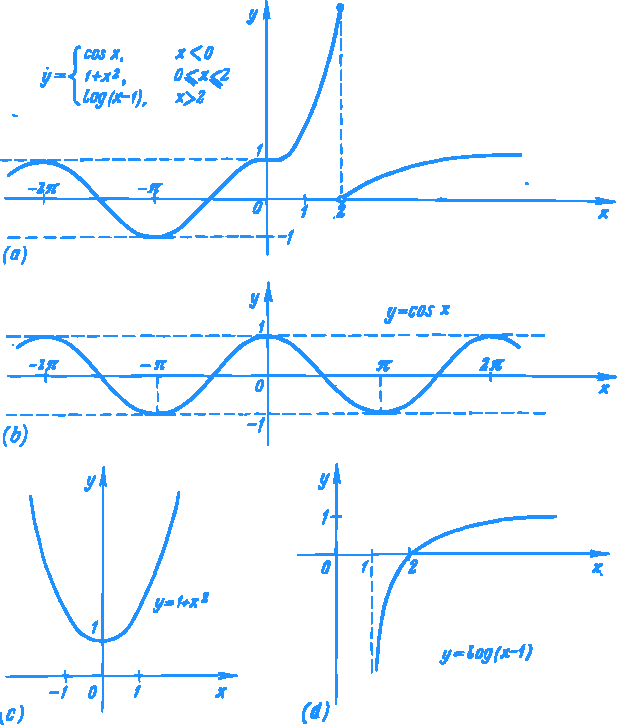
\includegraphics[width=\textwidth]{figures/fig-14.pdf}
\caption{The graphs of the functions $y = \cos x, \, y = 1 +x^{2}$, and $y = \log \, (x -1)$.}
\label{fig-14}
\end{figure}

\rdr In \fig{fig-14}\textcolor{IndianRed}{($a$)} I notice an open circle. What does it mean?

\athr This circle graphically represents a point excluded from the graph. In this particular case the point $(2, 0)$ does not belong to the graph of the function.
\fig{fig-15} plots the graphs of the functions that were discussed at the end of the previous dialogue. Let us have a close look at them.

\begin{figure}[!h]
\centering
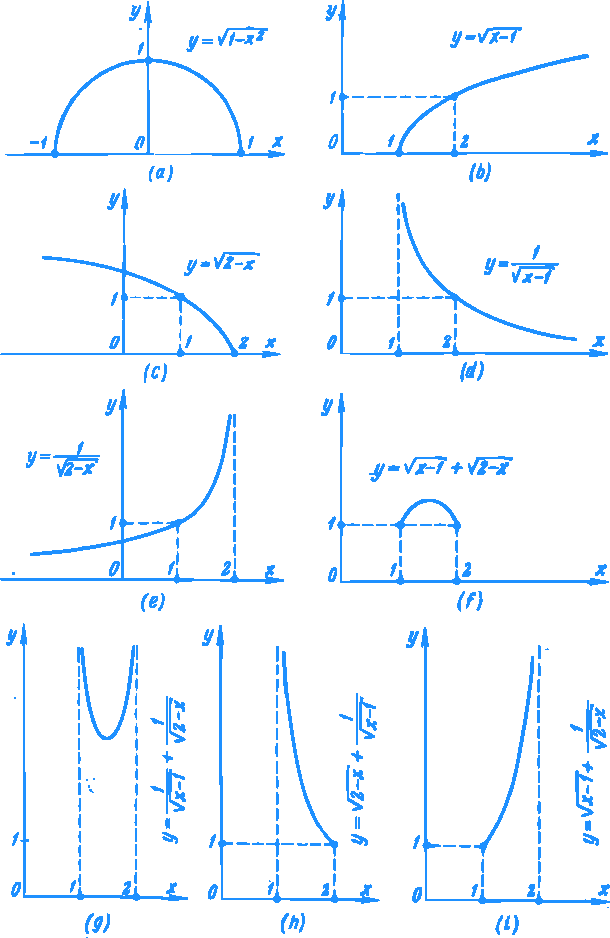
\includegraphics[width=0.85\textwidth]{figures/fig-15.pdf}
\caption{A variety of functions and their domains.}
\label{fig-15}
\end{figure}

\rdr Obviously, in all the cases shown in \fig{fig-15} the domain of the function is supposed coinciding with the domain of the corresponding analytical expression.

\athr Yes, you are right. In cases ($b$), ($c$), ($d$), and ($e$) these domains are infinite intervals. Consequently, only a part of each graph could be shown.

\rdr In other cases, however, such as ($g$), ($h$), and ($i$), the domains of the functions are intervals of finite length. But here as well the figure has space for only a part of each graph.

\athr That is right. The graph is presented in its complete form only in cases ($a$) and ($f$). Nevertheless, the behaviour of the graphs is quite clear for all the functions in \fig{fig-15}.

The cases which you noted, i.e. ($g$), ($h$), and ($i$), are very interesting. Here we deal with the unbounded function defined over the finite interval. The notion of boundedness (unboundedness) has already been discussed with respect
to numerical sequences (see \hyperref[infinite-seq]{Dialogue One}). Now we have to extrapolate this notion to functions defined over intervals.
\begin{mytheo}{Definition}
A function $y = f (x)$ is called \emph{bounded} over an interval $D$ if one can indicate two numbers $A$ and $B$ such that 
\begin{equation*}
A \leqslant f (x) \leqslant B \quad \text{for all $x \in D$} .
\end{equation*}
\end{mytheo}
If not, the function	is called \emph{unbounded}. 

Note that within infinite intervals you may define both bounded and unbounded functions. You are familiar with examples of bounded functions: $y = \sin x$ and $y = \cos x$. Examples of unbounded functions are in \fig{fig-15} (cases ($b$),
($c$), ($d$), and ($e$)).

\rdr Over the intervals of finite length both bounded and unbounded functions may also be defined. Several illustrations of such functions are also shown in \fig{fig-15}: the functions in cases ($a$) and ($f$) are bounded; the functions in cases ($g$), ($h$), and ($i$) are unbounded.

\athr You are right.

\rdr I note that in the cases that I have indicated the bounded functions are defined over the closed intervals ($[-1, 1]$ for ($a$) and $[1, 2]$ for ($f$)), while the unbounded functions are defined both over the open and half-open intervals ($]1, 2[$ for ($g$), $]1, 2]$ for ($h$), and $[1, 2[$ for ($i$)).

\athr This is very much to the point. However, you should bear in mind that it is possible to construct bounded functions defined over open (half-open) intervals, and unbounded functions defined over closed intervals. Here are two simple illustrations:

\textcolor{IndianRed}{\textbf{Example 1:}}  $y= x^{2}  \quad 0 \leqslant x< 2$ \\
\textcolor{IndianRed}{\textbf{Example 2:}}  
\begin{equation*}%
y = 
\begin{cases}
 \dfrac{1}{x} &  0 \leqslant x< 2\\
 1 & x =0
\end{cases}
\end{equation*}

The graphs of these functions are shown in \fig{fig-16}. 
\begin{figure}[!h]
\centering
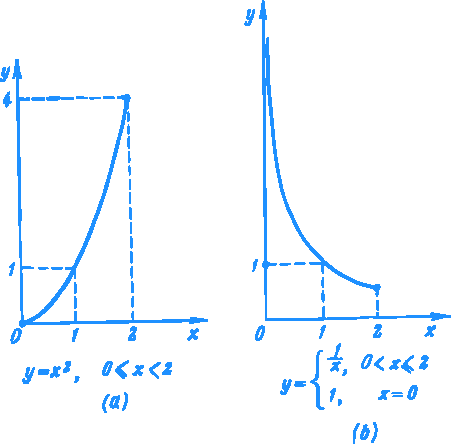
\includegraphics[width=0.75\textwidth,angle=-1]{figures/fig-16.pdf}
\caption{Examples of bounded functions defined over open (half-open) intervals, and unbounded functions defined over closed intervals.}
\label{fig-16}
\end{figure}

\rdr It seems that the boundedness (unboundedness) of a function and the finiteness of the interval over which it is defined are not interrelated, Am I right?

\athr Not completely. There is, for example, the following theorem.
\begin{mytheo}{Theorem}
If a function is defined over a closed interval and if it is monotonic, the function is bounded.
\end{mytheo}
\rdr Obviously, the monotonicity of a function is determined similarly to the monotonicity of a numerical sequence.

\athr Yes, it is. Monotonic functions can be classified, as sequences, into non-decreasing and non-increasing:
\begin{mytheo}{Definition}
\label{monotonic-def}
A function $y = f (x)$ is said to be \emph{non-decreasing} over an interval $D$ it for any $x_{1}$ and $x_{2}$ from this interval $f(x_{1}) \leqslant 
 f(x_{2})$ if $(x_{1} \leqslant  x_{2}$.  If, however, $f(x_{1}) \geqslant 
 f(x_{2})$, the function is said to be \emph{non-increasing}.
\end{mytheo}
Can you prove the theorem formulated above? 

\rdr Let the function $y = f (x)$ be defined over the closed interval $[a, b]$. We denote $f (a) = y_{a}$ and $f (b) = y_{b}$. To make the case more specific, let us assume that the function is non-decreasing. It means that $y_{a} \leqslant y_{b}$. I don't know how to proceed.

\athr Select an arbitrary point $x$ over the interval $[a, b]$.

\rdr Since $a \leqslant x$ and $x \leqslant b$, then, according to the condition of the above theorem, $y_{a} \leqslant f(x)$ and $f(x) \leqslant y_{b}$. Thus, we get that $y_{a}  \leqslant f(x) \leqslant y_{b} $ for all $x$ in the domain of the function. This completes the proof. 

\athr Correct. So, if a \emph{monotonic} function is defined over a closed interval, it is bounded. As to a \emph{non-monotonic} function defined over a closed interval, it may be either
bounded (\fig{fig-15}\textcolor{IndianRed}{($a$)} and ($f$)) or unbounded (\fig{fig-15}\textcolor{IndianRed}{($b$)}). 

And now answer the following question: Is the function $y = \sin x$ monotonic? 

\rdr No, it isn't. 

\athr Well, your answer is as vague as my question. First we should determine the domain of the function. If we consider the function $y = \sin x$ as defined on the natural domain (on the real line), then you are quite right. If, however, the domain of the function is limited to the interval $\left[-\dfrac{\pi}{2}, \dfrac{\pi}{2} \right]$ the function becomes monotonic (non-decreasing).

\rdr I see that the question of the boundedness or monotonicity of any function should be settled by taking into account both the type of the analytical expression for the function and the interval over which the function is defined.

\athr This observation is valid not only for the boundedness or monotonicity but also for other properties of functions. For example, is the function $y = 1 - x^{2}$ an \emph{even} function?

\rdr Evidently the answer depends on the domain of the function.

\athr Yes, of course. If the function is defined over an interval symmetric about the origin of coordinates (for example, on the real line or over the interval $[-1, 1]$), the graph of the function will be symmetric about the straight line $x= 0$. In this case $y= 1- x^{2}$ is an even function. If, however, we assume that the domain of the function is $[-1, 2]$, the symmetry we have discussed above is lost (\fig{fig-17}) and, as a result, $y = 1 - x^{2}$ is not even.
\begin{figure}[!ht]%{r}{0.5\textwidth}
\centering
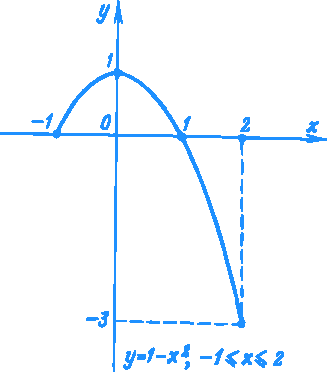
\includegraphics[width=0.5\textwidth,angle=1]{figures/fig-17.pdf}
\caption{ Is the function $y = 1 - x^{2}$  \emph{even}?}
\label{fig-17}
\end{figure}


\rdr It is obvious that your remark covers the case of odd functions as well.

\athr Yes, it does. Here is a rigorous definition of an even function.
\begin{mytheo}{Definition}
A function $y= f (x)$ is said to be \emph{even} if it is defined on a set $D$ symmetric about the origin and if $f (-x) = f (x)$ for all $x \in D$.
\end{mytheo}
By substituting $f (-x) = -f(x)$ for $f (-x) = f (x)$, we obtain the definition of an odd function.

But let us return to monotonic functions. If we drop the equality sign in the definition of a monotonic function (see p.~\pageref{monotonic-def}) (in $f (x_{1}) \leqslant f (x_{2})$ or $f (x_{1}) \leqslant f (x_{2})$), we obtain a so-called \emph{strictly monotonic function}. In this case a non-decreasing function becomes an \emph{increasing function} (i.e. $f (x_{1}) < f (x_{2})$) . Similarly, a non-increasing function becomes a \emph{decreasing function} (i.e. $f (x_{1}) > f (x_{2})$ ). In all the previous illustrations of monotonic functions we actually dealt with strictly monotonic functions (either increasing or decreasing).
\begin{figure}[!h]
\centering
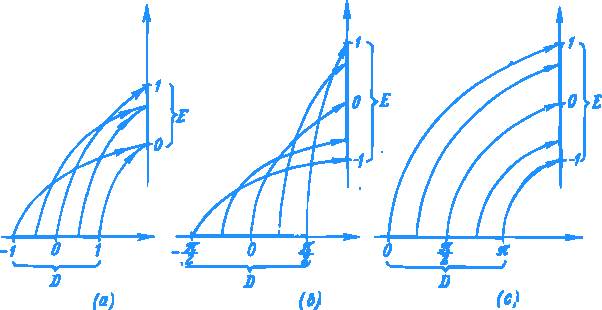
\includegraphics[width=\textwidth]{figures/fig-18.pdf}
\caption{ Concept of an \emph{inverse} function.}
\label{fig-18}
\end{figure}
Strictly monotonic functions possess an interesting property: \emph{each has an inverse function}.

\rdr The concept of an \emph{inverse function} has already been used in the previous dialogue in conjunction with the possibility of mapping a set of equilateral triangles onto a set of circles. We saw that the \emph{inverse mapping}, i.e. the mapping of the set of circles onto the set of equilateral triangles, was possible.

\athr That's right. Here we shall examine the concept of an inverse function in greater detail (but for numerical functions). Consider \fig{fig-18}. Similarly to the graphs presented in \fig{fig-13}, it shows three functions:

\begin{tabular}{lll}
%\begin{enumerate}[label=(\alph*), leftmargin=2cm]
(a) & $y= \sqrt{1-x^{2}}$ & $-1 \leqslant x \leqslant 1$ \\
(b) & $y= \sin x$ &   $- \dfrac{\pi}{2} \leqslant x \leqslant \dfrac{\pi}{2}$\\
(c) & $y= \cos x$ &  0 $\leqslant x  \leqslant  \pi$
%\end{enumerate}
\end{tabular}

Here we have three mappings of one numerical set onto another. In other words, we have three mappings of an interval onto another interval. In case (a) the interval $[-1, 1]$ is mapped onto the interval $[0, 1]$; in (b) the
interval $\left[-\dfrac{\pi}{2}, \dfrac{\pi}{2} \right]$ is mapped onto the interval $[-1, 1]$; and in (c) the interval $[0, \pi]$ is mapped onto the interval $[-1, 1]$.
What is the difference between mappings (b) and (c), on the one hand, and mapping (a), on the other?

\rdr In cases (b) and (c) we have a one-to-one correspondence, i.e. each point of the set $D$ corresponds to a single point of the set $E$ and vice versa, i.e. each point of $E$ corresponds to only one point of $D$. In case (a), however, there is no one-to-one correspondence.

\athr Yes, you are right. Assume now that the directions of all the arrows in the figure are reversed. Now, will the mappings define a function in all the three cases?

\rdr Obviously, in case (a) we will not have a function since then the reversal of the directions of the arrows produces a forbidden situation, namely, one number corresponds to two numbers. In cases (b) and (c) no forbidden situation occurs so that in these cases we shall have some new functions.

\athr That is correct. In case (b) we shall arrive at the function $y = \arcsin x$, which is the inverse function with respect to $y = \sin x$ defined over the interval $\left[-\dfrac{\pi}{2}, \dfrac{\pi}{2} \right]$.

In case (c) we arrive at the function $y =\arccos x$, which is the inverse function with respect to $y = \cos x$ defined over $[0, \pi]$.

I would like to place more emphasis on the fact that in order to obtain an inverse function from an initial function, it is necessary to have a one-to-one correspondence between the elements of the sets $D$ and $E$. That is why the functions $y = \sin x$ and $y = \cos x$ were defined not on their natural domains but over such intervals where these functions are either increasing or decreasing. In other words, the initial functions in cases (b) and (c) in \fig{fig-18} were defined as strictly monotonic. A strict monotonicity is a \emph{sufficient
condition} for the above-mentioned one-to-one correspondence between the elements of $D$ and $E$. No doubt you can prove without my help the following
theorem.
\begin{mytheo}{Theorem}
If a function $y = f(x)$ is strictly monotonic, different $x$ are mapped onto different $y$.
\end{mytheo}
\rdr Thus, a sufficient condition for the existence of the inverse function- is the strict monotonicity of the initial function. Is this right?

\athr Yes, it is.

\rdr But isn't the strict monotonicity of the initial function also a \emph{necessary condition} for the existence of the inverse function?

\athr No, it is not. A one-to-one correspondence may also take place in the case of a non-monotonic function. For example,
\begin{equation*}%
y = 
\begin{cases}
1 - x & 0 < x < 1 \\
x & 1 \leqslant x \leqslant 2
\end{cases}
\end{equation*}
Have a look at the graph of this function shown in \fig{fig-19}. If a function is strictly monotonic, it has the inverse function. However, the converse is not true. 

\begin{figure}[!ht]%[13]{r}{0.5\textwidth}
\centering
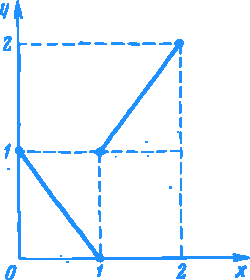
\includegraphics[width=0.48\textwidth]{figures/fig-19.pdf}
\caption{A non-monotonic function.}
\label{fig-19}
\end{figure}

\rdr As I understand it, in order to obtain an inverse function (when it exists), one should simply reverse the roles of $x$ and $y$ in the equation $y = f (x)$ defining the initial function. The inverse function will then be 'given by the equation $x = F (y)$. As a result the range of the initial function becomes the domain of the inverse function.

\athr That is correct. In practice a conversion of the initial function to the inverse function can be easily performed on a graph. The graph of the inverse function is
always \emph{symmetric} to the graph of the initial function about a straight line $y = x$. It is illustrated in \fig{fig-20}, which shows several pairs of graphs of the initial and inverse functions. A list of some pairs of functions with their domains is given below:


\begin{center}
\begin{tcolorbox}[colback=white,colframe=DodgerBlue]
\centering
%\boxed{
$\begin{array}{l>{\color{IndianRed}}cc>{\color{IndianRed}}cc}
\arrayrulecolor{DodgerBlue}
%\hline
 & \textbf{Initial} & \textbf{Domain} & \textbf{Inverse} & \textbf{Domain} \\
 \midrule
(a) & x^{3}& -\infty < x < \infty &\sqrt[3]{x} & -\infty < x < \infty\\
(b) & x^{2} & 0 \leqslant x < \infty & \sqrt{x} & 0 \leqslant x < \infty\\
(c) & 10^{x} & -\infty < x < \infty & \log x &  0 < x < \infty\\
(d) & \sin x & -\dfrac{\pi}{2}  \leqslant x  \leqslant \dfrac{\pi}{2} & \arcsin x & -1 \leqslant x \leqslant 1\\
(e) & \cos x & 0 \leqslant x \leqslant \pi & \arccos x & -1 \leqslant x \leqslant 1\\
(f) & \tan x & -\dfrac{\pi}{2}  < x  < \dfrac{\pi}{2}& \arctan x & -\infty < x < \infty \\
(g) & \cot x & 0 < x < \infty & \text{arccot}\, x &  -\infty < x < \infty\\[5pt]
%\midline
\end{array}$
%}
\end{tcolorbox}
\end{center}



All the domains of the inverse functions shown in the list case of are the natural domains of the functions (however, in the case of $y=\sqrt[3]{x}$ the natural domain is sometimes assumed to be restricted to the interval $[0, \infty[$ instead of the whole real line). As to the initial functions, only two of them ($y = x^{3}$ and $y = 10^{x}$) are considered in this case as defined on their natural domains. The remaining functions are defined over shorter intervals to ensure the strict monotonicity of the functions.

Now we shall discuss the concept of a \emph{composite function}.

Let us take as an example the function $h (x) =\sqrt{1 + \cos^{2} x}$. Consider also the functions $f (x) = \cos x$ and $g (y) = \sqrt{1+y^{2}}$.

\rdr This $f(x)$ notation is something new. So far we used to write $y = f (x)$,

\begin{figure}[!ht]%[13]{r}{0.5\textwidth}
\centering
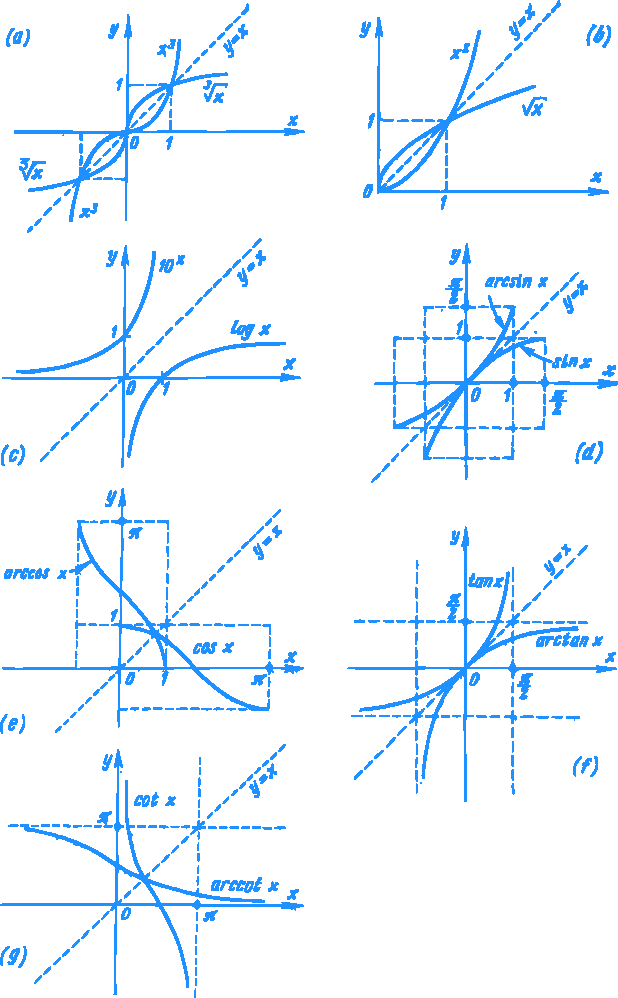
\includegraphics[width=0.85\textwidth]{figures/fig-20.pdf}
\caption{Functions and their inverses showing symmetry along the line $y=x$.}
\label{fig-20}
\end{figure}

\athr You are right. However, it is expedient to simplify the notation.

Consider the three functions: $h (x), \, f (x)$, and $g (y)$. The function $h (x)$ is a composite function composed of $f(x)$ and $g(y)$:
\begin{equation*}%
h (x) = g [f (x)] 
\end{equation*}
\rdr I understand. Here, the values of $f (x)$ are used as the values of the independent variable (argument) for $g (x)$.

\begin{figure}[!ht]%[13]{r}{0.5\textwidth}
\centering
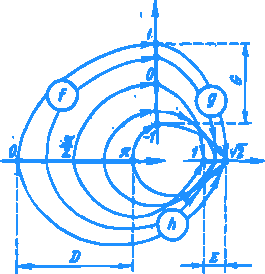
\includegraphics[width=0.5\textwidth]{figures/fig-21.pdf}
\caption{Understanding the composite function.}
\label{fig-21}
\end{figure}

\athr Let us have a look at \fig{fig-21}, which pictures the mappings of sets in the case of our composite function, $h (x) =\sqrt{1 + \cos^{2} x}$, with $f(x) = \cos x$ defined over the interval $[0, \pi]$.

We see that the function $f$ is a mapping of $D$ (the interval $[0, \pi]$) onto $G$ (the interval $[-1, 1]$), that is, the mapping $f$. The function $g$ (the function $\sqrt{1 + y^{2}}$) is a mapping of $G$ onto $E$ (the interval $[1, \sqrt{2}]$), that is, the mapping $g$. Finally, the function $h$ (the function $\sqrt{1 + \cos^{2} x}$ defined over the interval $[0, \pi]$) is a mapping of $D$ onto $E$, that is, the mapping $h$.

The mapping $h$ is a result of the consecutive mappings $f$ and $g$, and is said to be the composition of mappings; the following notation is used
\begin{equation*}%
h = g \circ f
\end{equation*}
(the right-hand side of the equation should be read from right to left: the mapping $f$ is used first and then the mapping $g$).

\rdr Obviously, for a composite function one can also draw a diagram shown in \fig{fig-22}.

\begin{figure}[!ht]%[13]{r}{0.5\textwidth}
\centering
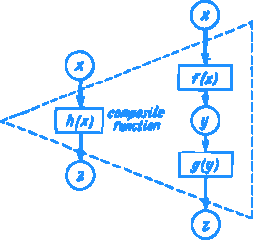
\includegraphics[width=0.5\textwidth]{figures/fig-22.pdf}
\caption{Understanding the composite function.}
\label{fig-22}
\end{figure}


\athr I have no objections. Although I feel that. we better proceed from the concept of a mapping of one set onto another, as in \fig{fig-21}.

\rdr Probably, certain ``difficulties'' may arise because the range of $f$ is at the. same time the domain of $g$? 

\athr In any case, this observation must always be kept in mind. One should not forget that the natural domain of a composite function $g [f (x)]$ is a portion (subset) of the natural domain of $f(x)$ for which the values of $f$ belong to the natural domain of $g$. This aspect was unimportant
in the example concerning $g [f (x)] = \sqrt{ 1 + \cos^{2} x}$ because all the values of $f$ (even if $\cos x$ is defined on the whole real line) fall into the natural domain of $g (y) = \sqrt{1 +y^{2}}$. I can give you, however, a different example:
\begin{equation*}%
h(x) = \sqrt{\sqrt{x-1} -2}, \quad f (x) = \sqrt{x-1}, \quad  g(y)=\sqrt{y -2}
\end{equation*}
The natural domain of $f (x)$ is $[1, \infty[$ Not any point in this interval, however, belongs to the domain of the composite function $h (x)$, Since the expression $\sqrt{y - 2}$ is meaningful only if $y \geqslant 2$, and for $y = 2$ we have $x = 5$, the natural domain of this composite function is represented by $[5, \infty]$, i.e. a subset smaller than the natural domain of $f (x)$.

Let us examine one more example of a composite function. Consider the function $y = \sin \,(\arcsin x)$, You know that $\arcsin x$ can be regarded as an angle the sine of which is equal to $x$. In other words, $\sin(\arcsin x) = x$, Can you point out the difference between the composite function $y = \sin \, (\arcsin x) $ and the function $y = x$?

\rdr Yes, I can. The natural domain of the function $y = x$ is represented by the whole real line. As to the composite function $y = \sin (\arcsin x)$, its natural domain coincides with the natural domain of the function $\arcsin x
$, i.e. with $[-1, 1]$. The graph of the function $y = \sin (\arcsin x)$ is shown in \fig{fig-23}.
\begin{figure}[!ht]%[13]{r}{0.5\textwidth}
\centering
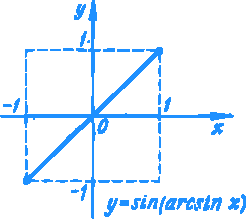
\includegraphics[width=0.5\textwidth]{figures/fig-23.pdf}
\caption{The graph of the function $y = \sin (\arcsin x)$.}
\label{fig-23}
\end{figure}

\athr Very good. In conclusion, let us get back to the problem of the graphical definition of a function. Note that there are functions whose graphs cannot be plotted in principle, the whole curve or a part of it. For example, it is impossible to plot the graph of the function $y= \sin \dfrac{1}{x}$ in the vicinity of $x = 0$ (\fig{fig-24}). It is also impossible to have the graph of the Dirichlet	function mentioned above.
\begin{figure}[!ht]%[13]{r}{0.5\textwidth}
\centering
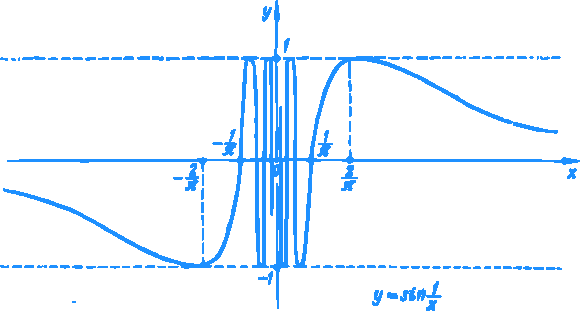
\includegraphics[width=\textwidth]{figures/fig-24.pdf}
\caption{The graph of the function $y = \sin \dfrac{1}{x}$.}
\label{fig-24}
\end{figure}

\rdr It seemed to me that the Dirichlet function had no graph at all. 

\athr No, this is not the case. Apparently, your idea of a graph of a function is always a curve.

\rdr But all the graphs that we have analyzed so far were curves, and rather smooth curves, at that.

\athr In the general case, such an image is not obligatory. But it should be stressed that \emph{every function has its graph, this graph being unique}.

\rdr Does this statement hold for functions that are not numerical

\athr Yes, it does. In the most general case we can give the following definition.
\begin{mytheo}{Definition}
The graph of a function $f$ defined on a set $D$ with a range on a set $E$ is a set of all pairs $(x, y)$ such that the first element of the pair $x$ belongs to $D$, while the second element of the pair $y$ belongs to $E$, $y$ being a function of $x \,\, (y= f(x))$.
\end{mytheo}

\rdr So it turns out that the graph of a function such as the area of a circle is actually a set of pairs each consisting of a circle (an element $x$) and a positive number (an element $y$) representing the area of a given circle.

\athr Precisely so. Similarly, the graph of a function representing a schedule of students on duty in a classroom is a set of pairs each containing a date (an element $x$) and the name of a student (an element $y$) who is on duty on this date. Note also that in practice this function indeed takes a graphic form.

If in a particular case both elements of the pair (both $x$ and $y$) are numbers, we arrive at the graph of the function represented by a set of points on the coordinate plane. This is the familiar graph of a numerical function.
}
% !TEX root = calculus.tex

\chapter{LIMIT OF FUNCTION}
{\parindent=0pt
\athr Consider now the concept of the limit of function.

\rdr But we have already covered rather extensively the concept of the limit of a numerical sequence. But a sequence is nothing else but a function defined on a set of natural numbers. Thus, having discussed the limit of sequence, we become acquainted with the limit of function as well. I wonder whether there is any point in a special discussion of the concept of the \emph{limit of function}.

\athr Undoubtedly, a further discussion will be very much to the point. The functions we are concerned with substantially differ from sequences (I have already emphasized this fact) because they are defined over \emph{intervals} and not on sets of natural numbers. This fact makes the concept
of the \emph{limit of function specific}. Note, for example, that every specific convergent sequence has only one limit. It means that the words ``the limit of a given sequence'' are self-explanatory. As for a function defined over an interval, one can speak of an infinite number of ``limits'' because the limit of function is found for each specific point $x = a$ (or, as we say, for $x$ tending to $a$). Thus the phrase ``the limit of a \emph{given} function'' is meaningless because ``the limit of a \emph{given} function must be considered only at each given point $a$''. Besides, this point a should either belong to the domain of the function or coincide with one of the ends of the domain.

\rdr In this case the definition of the limit of function should be very different from that of the limit of sequence.

\athr Certainly, there is a difference.

Note, first of all, that we analyze a function $y = f (x)$, which is defined over a segment, and a point a in this segment (which may coincide with one of its ends when the function is defined over an open or half-open interval).

\rdr Do you mean to say that at the point $x = a$ the function $f (x)$ may not be defined at all?

\athr That is quite correct. Now let us formulate the definition of the limit of function.
\begin{mytheo}{Definition}
A number $b$ is said to be the limit of a function $f (x)$ at $x$ tending to $a$ (the limit at point $a$) if for any positive value of $\varepsilon$ there is a positive value of $\delta$ such that for all $x$ satisfying the conditions $x$ belongs to the domain of the function; $x \neq a$ and 
\begin{equation}%
|x- a| < \delta
\label{lim-delta}
%eq-1
\end{equation}
we have
\begin{equation}%
\left|f(x)- b \right| < \varepsilon
\label{lim-eps}
%eq2
\end{equation}
\end{mytheo}
The standard notation is
\begin{equation*}%
\lim\limits_{x \to a} f (x) = b
\end{equation*}

\rdr The definition of the limit of function is noticeably longer and more complicated than that of the limit of sequence.

\athr Note, first of all, that according to \eqref{lim-delta}, point $x$ should	belong	to	the	interval	 $]a -\delta,	a + \delta[$. Point $x = a$ should be \emph{eliminated} from this interval. The interval $]a -\delta,	a + \delta[$ without point $x = a$ is called a \emph{punctured $\delta$-neighbourhood} of point $a$.

We select an arbitrary positive number $\varepsilon$. For $\varepsilon$ we want to find \emph{another} positive number $\delta$ such that the value of the function at \emph{any} point $x$ from the punctured $
\delta$-neighbourhood of point a must be inside the interval  $]b -\varepsilon,	b + \varepsilon [$ (speaking about \emph{any} point $x$ we imply only the points $x$ in the domain of the function). If there is such $b$ for any $\varepsilon > 0$, $b$ is said to be the limit of the function at point $a$. Otherwise, $b$ is not the limit of the function at point $a$.

\rdr And what does your ``otherwise'' mean in practice?

\athr Assume that the search for $\delta$ has been successful for $n$ diminishing numbers $\varepsilon_{1}, \, \varepsilon_{2}, \, \ldots, \, \varepsilon_{n}$. But then you notice that for a certain number $\varepsilon'$ it is impossible to find the required number $\delta$, i.e. for any value of $\delta$ no matter
how small) there is \emph{always at least one} point $x$ from the punctured $\delta$-neighbourhood of point $a$ at which the value of the function \emph{lies outside} the interval $]b -\varepsilon\,	\, b + \varepsilon' [$.

\rdr But can it happen that we reduce the $\delta$-neighbourhood of point a so much that not a single point $x$, belonging to the domain of the function, remains in the $\delta$-neighbourhood?

\athr Obviously this is impossible. Because the function is defined over an interval, and point $a$ is taken either from this interval or coincides with its end point.

\rdr Everything seems clear. Apparently, in order to root all this firmly in my mind we should discuss the graph of a function.


\athr It is a good idea. Let us analyze, for the sake of convenience, the graph of the function $y = \sqrt{x}$ (\fig{fig-25}). This figure illustrates only two situations. One of them represents the selection of $\varepsilon_{1}$ (see the figure). It is easy to infer that $\delta_{1}$	is the value that we look for: the values of the function at all points $x$ from the $\delta_{1}$-neighbourhood of point a
are inside the interval $]b -\varepsilon_{1} 	\, b + \varepsilon_{1} [$ These values are represented by the portion of the graph between points $A$ and $B$. The second situation represents the selection of $\varepsilon_{2}$.

\begin{figure}[!ht]%[13]{r}{0.5\textwidth}
\centering
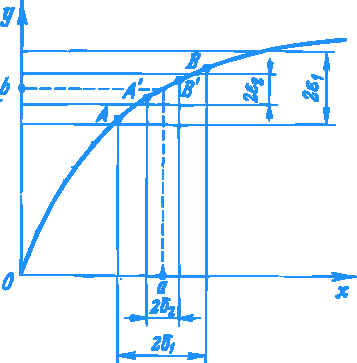
\includegraphics[width=0.6\textwidth]{figures/fig-25.pdf}
\caption{Understanding limit of the function $y = \sqrt{x}$.}
\label{fig-25}
\end{figure}

In this case the number that we seek for is $\delta_{1}$: the values of the function at points $x$ from the $\delta_{2}$-neighbourhood of point a are represented by the portion of the graph between points $A'$ and $B'$.

\rdr Everything you have just described looks so obvious that I see no ``cream'', to use your own words. 

\athr ``The cream'' consists in the following. No matter how small $]b -\varepsilon 	\, b + \varepsilon [$ is, one may always select a $\delta$-neighbourhood for point $a$ such that for all points $x$ in this $\delta$-neighbourhood (all points, with the exception of point $a$ itself and those at which the function is not defined) the values of the function should by all means lie within the indicated interval.

\rdr Could you give an example of a function violating this rule?

\athr For instance, the function $y = \sin \dfrac{1}{x}$ in the
vicinity of point $x = 0$. The graph of the function is plotted in \fig{fig-24}. Obviously, the smaller is $|x|$ the greater is the frequency with which the graph of the function oscillates about the $x$-axis. For an infinitely small $|x|$ the frequency of the oscillations tends to infinity. It is easy to prove that
the function $y = \sin \dfrac{1}{x}$ has no limit at $x = 0$.

\rdr But this function is not defined at zero.

\athr You are right. However, this fact is irrelevant from the viewpoint of the existence (or absence) of the limit of the function at $x = 0$. This function is defined over $]-\infty, 0[$ and $]0, \infty[$. Point $x = 0$ is a common boundary between the intervals over which the function $\sin \dfrac{1}{x}$ is defined. 

But let us return to the concept of the limit. Can we,
for example, state that $b = 0$ is the limit of the function $\sin \dfrac{1}{x}$ at point $x = 0$?

\rdr It seems that I get the point. As long as we
select $\varepsilon > 1$, everything is O.K. But for any $\varepsilon < 1$ it becomes impossible to find a	$\delta$-neighbourhood of	point $x = 0$ such that at all points $x \neq 0$ in this $\delta$-neighbourhood
the values of the function $\sin \dfrac{1}{x}$  are inside the interval
]-8, e]. No matter how \emph{small} the $\delta$-neighbourhood of point $x = 0$ is, it is the segment of \emph{finite} length, so that the graph of our function will oscillate \emph{infinitely many times} and thus will \emph{infinitely many times} go \emph{beyond} $]-\varepsilon,	\, \varepsilon [$.

\athr That's right. Note also that in order to be convinced that a function has no limit, it is sufficient to find a violation even more ``modest''. Namely, it is sufficient that the graph of the function leave the interval $]-\varepsilon,	\, \varepsilon [$ \emph{at least once} for any $\delta$-neighbourhood.

\rdr Apparently, not only $b = 0$ but no other $b \neq 0$ can be the limit of the function $y = \sin \dfrac{1}{x}$ at $x= 0$. Because for any $b \neq 0$ we can use the same arguments as for $b = 0$.

\athr Hence, we have proved that the function $y = \sin \dfrac{1}{x}$ has no limit at point $x=0$.

\rdr The reason for the absence of the limit at $x= 0$ lies in oscillations of the graph of the function. These oscillations become more and more frequent while approaching $x= 0$.

\athr But the reason is not confined only to the infinitely increasing frequency of oscillations of the graph. Another reason is the constancy of the amplitude of oscillations. Let us ``slightly correct'' our function by multiplying
$\sin \dfrac{1}{x}$ by $x$, The graph of the function $y = x \sin \dfrac{1}{x}$ is shown in \fig{fig-26}. Do you think that $b= 0$ is the limit of this function at $x = 0$?

\begin{figure}[!ht]%[13]{r}{0.5\textwidth}
\centering
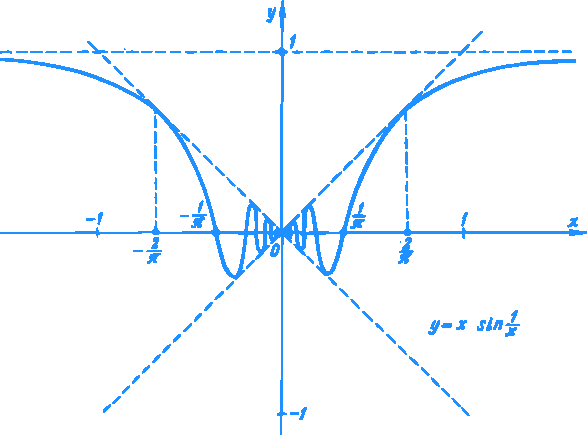
\includegraphics[width=\textwidth]{figures/fig-26.pdf}
\caption{Finding the limit of the function $y = x \sin \dfrac{1}{x}$.}
\label{fig-26}
\end{figure}

\rdr I am at a loss.

\athr I'll answer this question myself. Yes, it is. The proof is within your reach if you use the definition of the limit of function. You are welcome.


\rdr We select an arbitrary $\varepsilon > 0$. We should find $\delta > 0$such that $\left| x \sin \dfrac{1}{x} -0 \right|< \varepsilon$ for all $x$ (excluding $x = 0$) satisfying the condition $|x - 0 |< \delta$. It seems
to me that $\delta$ we look for is $\delta = \varepsilon$.

\athr You are quite right. Because if  $|x| < \delta = \varepsilon$, it becomes evident that $\left| x \sin \dfrac{1}{x}\right| = |x| \left| \sin \dfrac{1}{x} \right| < \varepsilon$.
(since $\left| \sin \dfrac{1}{x} \right| \leqslant 1$). 

\rdr Really, the existence of the limit is proved
without considerable difficulties. 

\athr But, certainly, not always. Consider, for
example, a well-known function $y = \sqrt{x}$ and prove (using the definition of the limit of function) that $b = 1$ is the limit of the function at point $x = 1$.
To begin with, consider the following inequality:
\begin{equation*}%
\left|\sqrt{x} -1  \right| < \varepsilon
\end{equation*}
Try to find a function $g(\varepsilon)$ such that $\left|x - 1 \right|<g(\varepsilon)$
for any $x$ satisfying the condition  $\left|\sqrt{x} - 1 \right|< \varepsilon$

\rdr I understand that $g(\varepsilon)$ is actually the desired $\delta$ 6 corresponding to an arbitrary $\varepsilon$.

\athr Yes, of course. We begin with some transformations. We shall proceed from the inequality:
\begin{equation}%
\left|\sqrt{x} -1 \right| < \varepsilon
\label{ineq-1}
%eq-3
\end{equation}
which can be rewritten in the form:
\begin{equation*}%
(1 - \varepsilon) < \sqrt{x} < (1+ \varepsilon)
\end{equation*}
Since $\sqrt{x} \geqslant 0$, the selection of $\varepsilon < 1$ \emph{a fortiori} (which, of course, does not impair the generality of our proof) allows us to square the last inequalities
\begin{equation*}%
(1 - \varepsilon)^{2} < x < (1+ \varepsilon)^{2}
\end{equation*}
 On removing the parentheses, we obtain
\begin{equation}%
(-2\varepsilon - \varepsilon^{2}) < (x -1) < (2\varepsilon + \varepsilon^{2})
\label{ineq-2}
%eq-4
\end{equation}
Note that inequalities \eqref{ineq-2} are equivalent to \eqref{ineq-1} (provided that $0< \varepsilon < 1$). Now let us proceed from \eqref{ineq-2} to a more exacting inequality:
\begin{equation}%
|x -1| < (2\varepsilon - \varepsilon^{2})
\label{ineq-3}
%eq-5
\end{equation}
(since $0< \varepsilon < 1$, we have $(2\varepsilon - \varepsilon^{2}) > 0$). It is easy to conclude that if \eqref{ineq-3} holds, inequalities \eqref{ineq-2} and, consequently \eqref{ineq-1} will hold all the more. Thus, for an arbitrary $\varepsilon$ within $0< \varepsilon < 1$, it is sufficient to take $\delta = 2 \varepsilon - \varepsilon^{2}$

\rdr What happens if $\varepsilon \gg 1$? 

\athr Then $\delta$ determined for any $\varepsilon < 1$ will be adequate \emph{a fortiori}. 

\rdr Apparently, we may state that
\begin{equation*}%
\lim\limits_{x \to 2} \sqrt{x} = \sqrt{2}, \quad \lim\limits_{x \to 3} \sqrt{x} = \sqrt{3}
\end{equation*}
and, in general, $\lim\limits_{x \to a} \sqrt{x} = \sqrt{a}$.

\athr Yes, that's right. 

\rdr But could we generalize it to
\begin{equation*}%
\lim\limits_{x \to a} f(x) = f(a)
\end{equation*}

\athr Yes, it is often the case. But not always. Because the function $f (x)$ may be undefined at point $a$.
Remember that the limit of the function $y = x \sin \dfrac{1}{x}$ at point
$x = 0$ is zero, but the function itself is not defined at point $x = 0$.

\rdr But perhaps the equality lim f (x) = f (a) x~a
can be considered as valid in all the cases when f (x) is defined at point a?

\athr This may not be correct either. Consider, for example, a function which is called the ``fractional part of $x$''. The standard notation for this function is $\{x\}$. The function is defined on the whole real line. We shall divide the real line into half-intervals $[n, n + 1[$. For $x$ in $[n, n + 1[$ we have $\{x\} = x- n$. The graph of the function $y = \{x\}$ is shown in \fig{fig-27}.

\begin{figure}[!ht]%[13]{r}{0.5\textwidth}
\centering
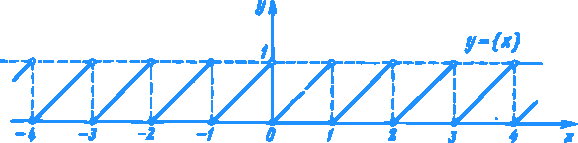
\includegraphics[width=\textwidth]{figures/fig-27.pdf}
\caption{Graph of the function $y = \{x\}$.}
\label{fig-27}
\end{figure}
Take, for example, $x = 1$. It is obvious that $\{x\}$ is defined at point $x = 1 (\{x\} = 0)$. But does the function have the limit at $x = 1$?

\rdr It clearly has no limit. In any $\delta$-neighbourhood of point $x = 1$ there may exist concurrently both the points at which $\{x\}$ assumes values greater than, for example, $\dfrac{2}{3}$, and the points at which $\{x\}$ assumes values less than $\dfrac{1}{3}$.

It means that neither $b= 1$ nor $b=0$ can be the limit of the function at point $x = 1$, if only because it is impossible to find an adequate $\delta$ for  $\varepsilon =\dfrac{1}{3}$.

\athr I see that you have come to be rather fluent in operating with limits of functions. My compliments.

By the way, you have just proved the theorem on the \emph{uniqueness of the limit of function} at a given point.
\begin{mytheo}{Theorem}
A function cannot have two (or more) limits at a given point.
\end{mytheo}
Now let us return to the equality
\begin{equation}%
\lim\limits_{x \to a} f(x) = f(a)
\label{fn-limit}
%eq-06
\end{equation}
You already know that there are situations when $\lim\limits_{x \to a} f(x)$ exists but $f (a)$ does not exist and, vice versa, when $f (a)$
exists but $\lim\limits_{x \to a} f(x)$ does not exist. Finally, a situation is
possible when both $\lim\limits_{x \to a} f(x)$ and $f (a)$ exist, but their 
values are not equal. I'll give you an example: 
\begin{equation*}%
f(x)=
\begin{cases}
 x^{2} & \text{if} \,\, x \neq 0\\
 1 & \text{if} \,\, x=0
 \end{cases}
 \end{equation*}
  The graph of this function is shown in \fig{fig-28}. It is easy
to see that $f(0) = 1$, while $\lim\limits_{x \to a} f(x) =0$.
  
  \begin{figure}[!ht]%[13]{r}{0.5\textwidth}
\centering
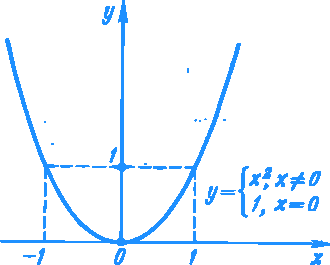
\includegraphics[width=.6\textwidth]{figures/fig-28.pdf}
\caption{Graph of the function $y = f(x)$, such that $f(x) = x^{2}$ for $x \neq 0$ and $f(x) = 1$ for $x = 0$.}
\label{fig-28}
\end{figure}
You must be convinced by now that equality \eqref{fn-limit} is not always valid.

\rdr But presumably, it is often true, isn't it?

\athr Yes, and if it is, the function $f (x)$ is said to be \emph{continuous} at $x = a$.

Thus, we have arrived at a new important concept, namely, that of the \emph{continuity of a function at a point}. Let us give the following definition.
\begin{mytheo}{Definition}
A function $f (x)$ is said to be \emph{continuous at a point} $x = a$ if 
\begin{enumerate}[leftmargin=2cm,label=\protect\circled{\arabic*}]
\item it is defined at $x = a$, 
\item there is the limit of the function at $x = a$, 
\item this limit equals the value of the function at $x = a$;
\end{enumerate}
or, in other words, the function $f (x)$ is called continuous at a point $a$ if
\begin{equation*}%
\lim\limits_{x \to a} f(x) = f(a)
\end{equation*}
\end{mytheo}

I believe that the preceding discussion has brought us so closely to this definition that it needs no additional explanation. I would only like to emphasize that the concept of the continuity of a function is essentially \emph{local}. Similarly to the concept of the limit of function, it is related to a particular point $x$. A function may be either continuous at all points of an interval over which it is defined, or discontinuous at some of its points.

Taking the examples given above, can you single out those functions that are discontinuous at particular points?

\rdr To begin with, I may refer to the function whose graph is plotted in \fig{fig-28}. This function is discontinuous at $x = 0$.

\athr Why?

\rdr Because at this point the function assumes the value $y = 1$, though the limit of the function at this point is apparently zero.

\athr Very good. Can you give other examples?

\rdr The function $y = \{x\}$ (see \fig{fig-27}) is discontinuous at points $x = 0, \,\pm 1, \, \pm2, \, \pm3, \ldots$ The function $y = \sin \dfrac{1}{x}$ (see \fig{fig-24}) is discontinuous at $x = 0$ where it is undefined and, moreover, has no limit. The function whose graph is shown in \fig{fig-14}\textcolor{IndianRed}{($a$)} (see the previous, dialogue) is discontinuous at $x = 2$. The function $y = \tan x$ is discontinuous at points 
\begin{equation*}%
x = \pm \frac{\pi}{2}, \,\, \pm \frac{3\pi}{2}, \,\, \pm \frac{5\pi}{2}, \,\, \pm \frac{7 \pi}{2}
\end{equation*}

\athr That will do. Note that the points at which the continuity of a function is violated are called \emph{discontinuity points}. We say that at these points a function has a discontinuity. In passing through a discontinuity point a graph of a function manifests a singularity. This fact is well illustrated by the examples you have just indicated,

\rdr The discontinuity points in all these examples result in an \emph{interruption of the curve} plotting the function.
One exception is the function  $y = \sin \dfrac{1}{x}$  since it is simply impossible to trace a graph of the function at $x = 0$. 

\athr I may add that neither could you plot the function $y = \tan x$ at its discontinuity points (since you cannot draw a line which ``goes into infinity''). 

\rdr In any case, if a function is continuous everywhere in the domain (has no discontinuity points), its graph is a continuous line: it can be drawn without lifting
the pencil from the paper. 

\athr I agree. I would like to emphasize that the \emph{continuity of a function at a point $x$ guarantees that a very small displacement from this point will result in a very small change in the value of the function}.

Let us turn to \fig{fig-27} which is the graph of the function $y = \{x\}$. Consider, for instance, $x = 0.5$. The function is continuous at this point. It is quite evident that at a very small displacement from the point (either to the left or to the right) the value of the function will also change only a little. Quite a different situation is observed if $x = 1$ (at one of the discontinuity points). At $x = 1$ the function assumes the value $y = 0$. But an infinitesimal shift \emph{to the left} from the point $x = 1$ (take, for example, $x = 0.999$, or $x = 0.9999$, or any other point no matter how close to $x = 1$) will bring a sharp change in the value of the function, from $y= 0$ to $y \approx 1 $.

\rdr Quite clear. I must admit, however, that the local nature of the concept of a continuous function (i.e. the fact that the continuity of a function is always related to a specific point $x$) does not quite conform to the conventional idea of continuity. Because continuity typically implies a process and, consequently, a sort of an interval. It seems that continuity should be related not to a specific moment of time, but to an interval of time.

\athr It is an interesting observation. This local character is a manifestation of one of the specific features of calculus. When analyzing a function at a given point $x$, you used to speak about its value only at this specific point; but calculus operates not only with the value of a function at a point but also with the limit of the function (or its absence) at this point, with the continuity of the function at the point. It means that on the basis of the information about a function at a given point we may construct an image of the \emph{behaviour of the function in the vicinity of this point}. Thus we can predict the behaviour of the function if the point is slightly shifted from $x$.

So far we have made only the first step in this direction. The next step will be the introduction of the concept of a derivative. This will be the subject of discussion in \hyperref[velocity]{Dialogues Eight} and \hyperref[derivative]{Nine}.

\rdr Nevertheless, I would like to note that in the above examples a function was found to be either continuous everywhere over any interval of finite length or discontinuous at a \emph{finite} number of points. In this sense the local nature of the concept of a discontinuity point is evident. The continuity of the function, however, is always observed over a certain interval.

\athr First, the continuity of a function within an interval does not interfere with the local nature of continuity. \emph{A function is continuous over an interval if it is continuous at all points of this interval.}

Second, it is not difficult to construct an example in which the number of discontinuity points over an interval of finite length is \emph{infinitely large}. Let us look, for example, at the following function:
\begin{equation*}%
y =
\begin{cases}
2 & \,\, \text{for} \,\, x= \pm 1, \, \pm \dfrac{1}{2},\, \pm \dfrac{1}{4},\, \pm \dfrac{1}{8},\, \pm \dfrac{1}{16} \ldots \\
x^{2} & \,\, \text{for all the remaining points of the real line, including} \,\, x = 0
\end{cases}
\end{equation*}
The graph of this function is illustrated in \fig{fig-29}. It is easy to conclude that in any $\delta$-neighbourhood of point $x = 0$ the function has an infinite number of discontinuity points.
\begin{figure}[!ht]%[13]{r}{0.5\textwidth}
\centering
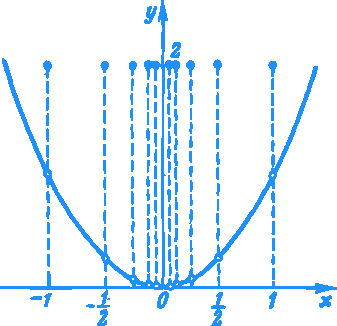
\includegraphics[width=.7\textwidth]{figures/fig-29.pdf}
\caption{Graph of the function $y = f(x)$, such that $f(x) = 2$ for $ x= \pm 1, \, \pm \dfrac{1}{2},\, \pm \dfrac{1}{4},\, \pm \dfrac{1}{8},\, \pm \dfrac{1}{16} \ldots $ and $f(x) = x^{2}$ for all the remaining points of the real line, including $x = 0$.}
\label{fig-29}
\end{figure}

Finally, I can give an example of a function which is discontinuous \emph{at all points of an infinite interval}. This is a function you already know, the Dirichlet function (see the previous dialogue). Being defined on the whole real line, the function has no limit at any point of the real line; consequently, it is discontinuous at each point.

\rdr This is the reason why we in principle cannot plot the Dirichlet function by a graph.

\athr As to the most frequent functions, such as \emph{power, exponential, logarithmic, trigonometric}, and \emph{inverse trigonometric}, they are continuous at all points of the natural domains of the corresponding analytical expressions. The same can be said about composite functions obtained from the above elementary functions. The continuity of all these functions is proved in the more advanced courses of calculus. We limit ourselves to a mere stating of the fact.
}
% !TEX root = calculus.tex

\chapter{MORE ON THE LIMIT OF FUNCTION}
\label{more-limit-func}
{\parindent=0pt
\rdr Comparing the definition of the limit of a function at a point with the definition of the limit of a numerical sequence, I come to the conclusion that these two limits are of different nature.

\athr And I understand why. In fact, I did emphasize the difference myself in the previous dialogue, pointing out, as you probably remember, that a sequence is a function defined on a set of integers, while the functions we are discussing at the moment are defined over intervals. I doubt, however, that you are justified in speaking about the difference in the nature of the limit of function and that of sequence. In the final analysis (and this is essential) \emph{the limit of a function at a point may be defined on the basis of the limit of a numerical sequence}.

\rdr This is very interesting.

\athr Let us forget, for the time being, about the definition of the limit of function given in the previous dialogue. Consider a new definition.
We shall consider, as before, a function, $f (x)$ defined over an interval, and a point $x = a$ either taken within the interval or coinciding with its end.

\athr The two are \emph{equivalent}. 

\rdr But in form they are quite different.

\athr We can prove their equivalence. To begin with, let the definition using a $\delta$-neighbourhood of point a be called ``definition \emph{1}'', and the definition using numerical sequences, ``definition \emph{2}''.

Now, what two theorems must be proved to demonstrate the equivalence of definitions \emph{1} and \emph{2}? Can you formulate these theorems?

\rdr We have to prove two theorems, one direct and the other converse. We want to prove that definition \emph{2} follows from definition \emph{1} and vice versa (i.e. definition \emph{1} follows from	definition \emph{2}).

\athr Correct. First, I shall prove the following theorem.
\begin{mytheo}{Theorem} If a number $b$ is the limit of a function $f (x)$ at a point $a$, in terms of definition \emph{1}, it is the limit of the function $f (x)$ at $a$ in terms of definition \emph{2} as well.
\end{mytheo}

Since $b$ is the limit of the function $f (x)$ at point a in terms of definition \emph{1} (this is given), consequently, for any $\varepsilon > 0$ there is $\delta > 0$ such that $| f(x)- b | < \varepsilon$  for all $x \neq a$ from a $\delta$-neighbourhood of point $a$. Then we ``construct''	an	arbitrary	sequence	($x_{n}$) ,	requiring	that	it	be convergent to point $a$ (any $x_{n}$ belong to the domain of the function and $x_{n} \neq a$ for any $n$). As a result we obtain a sequence of the corresponding values of the function (the sequence	$[f (x_{n} ) ]$) .	We	want	to	prove	that	the	sequence $[f (x_{n} )]$ is convergent to $b$.

First, I select an arbitrary $\varepsilon > 0$. I should find a number $N$ such that $|f(x_{n}) -	b| < \varepsilon$ for all $n > N$.

I cannot immediately find such $N$ for an arbitrary $\varepsilon$. However, I can indicate for an arbitrary $\varepsilon$ such $\delta$ that $| f(x)- b | < \varepsilon$  
if $|x- a| < \varepsilon$. Then I take this $\delta$ and find a sequence $(x_{n})$ convergent to $a$. Evidently, since $(x_{n})$ is convergent to $a$,  $\varepsilon$(as any other positive real number) can be placed in correspondence with a number $N$ such that $|x_{n} - a| < \delta$ for all $n > N$. And, consequently, we
also have that $|f(x_{n}) - b| < \varepsilon$ for all $n > N$. Hence we find that the thus found number $N$ is actually the desired number.	It proves	the	convergence	of	the	sequence $[f (x_{n} )]$ to	$b$. Since	the sequence	$(x_{n} )$,	which	is	convergent	to	$a$ was chosen (``constructed'') arbitrarily, we conclude that the theorem's proof is completed.

If the line of reasoning is clear to you, try briefly to recapitulate the logical 
structure of the proof.

\begin{figure}[!ht]%[13]{r}{0.5\textwidth}
\centering
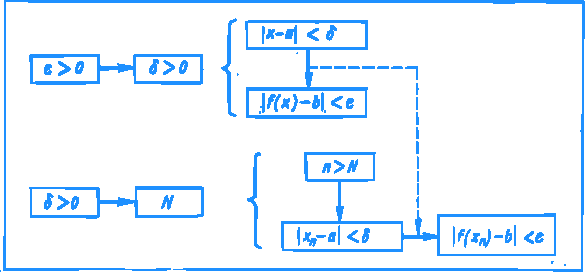
\includegraphics[width=\textwidth]{figures/fig-30.pdf}
\caption{Schematic diagram of the proof that two definitions of the limit of a function are equal.}
\label{fig-30}
\end{figure}

\rdr I shall try to present the structure of the proof as a diagram (\fig{fig-30}).

\athr Your diagram is correct. Will you expand on it. 

\rdr The \emph{first step} of the proof: we find for an arbitrary $\varepsilon
> 0$ a number $\delta > 0$ such that $| f(x)- b | < \varepsilon$ if $|x - a| < \delta$. 

The \emph{second step} of the proof: we take $\delta$ selected at the
first step; choose a sequence $(x_{n})$ convergent to $a$, and find a number $N$ such that  $|x - a| < \delta$ for all $n > N$. Having in mind the arguments used at the first step, we conclude that $| f(x)- b | < \varepsilon$. 

We have thus found for an arbitrary $\varepsilon > 0$ a number $N$ such that  $| f(x_{n})- b | < \varepsilon$ for all $n > N$. This completes the proof.

\athr Correct. In conclusion I want to emphasize several essential points on which the proof hinges. We know that $| f(x)- b | < \varepsilon$ for any $x$ from the $\delta$-neighbourood of $a$. Since a sequence $(x_{n})$ is convergent to $a$, all $x_{n}$ (the whole infinite ``tail'' of the sequence $(x_{n})$ starting from a certain number $N +1$) are contained inside the $\delta$-neighbourhood of point $a$. It then follows that all $f (x_{n} )$ (the whole infinite	``tail'' of the sequence $[f (x_{n} )]$ starting from the same number N + 1.) are contained inside the interval $] b - \varepsilon, b + \varepsilon[$, This proves that the sequence $[f (x_{n})]$ converges to $b$.

\rdr I understand.

\athr Now I am going to prove the following converse theorem.
\begin{mytheo}{Theorem}
If a number $b$ is the limit of a function $f (x)$ at a point $a$ in terms of definition \emph{2}, it is also the limit of the function $f (x)$ at a in terms of definition \emph{1}.
\end{mytheo}
In this case I shall use the proof by contradiction. Assume the contrary to what is to be proved, namely, assume that $b$, the limit of $f (x)$ in terms of definition \emph{2}, is not, however, the limit of $f (x)$ in terms of definition \emph{1}. Can you formulate the last proposition (more exactly, the assumption)?

\rdr As far as I remember, a similar formulation has already been discussed in the previous dialogue. If $b$ is not the limit of the function $f (x)$ at point $a$ (in terms of definition \emph{1}), it means that there is $\varepsilon' > 0$ such that it is impossible to find a necessary $\delta> 0$. Namely, no matter what $\delta$ we select, each time the function $f (x) $assumes a value outside of $]b - \varepsilon', \, b + \varepsilon'[$ for at least one point $x$ from the $\delta$-neighbourhood of point $a$, i.e. the inequality $| f(x)- b | < \varepsilon'$ is violated.

\athr Correct. Assume that we have selected precisely this $ \varepsilon' > 0$. Next take an arbitrary $\delta> 0$, for instance, $\delta_{1} = 1$. As you have said, in any $\delta$-neighbourhood of point $a$ and, hence, in the $\delta$-neighbourhood of this point there is at least one point $x$ (denoted by $x_{1}$) such that $|f(x_{1} -b|  \geqslant \varepsilon'$.

\rdr What happens if the $\delta$-neighbourhood contains many such points $x$? 

\athr It makes no difference. The important fact is that there is \emph{at least one such point}. If there are several such points, take anyone of them and denote it by $x_{1}$.

Now we take a new $\delta$, for instance, $\delta_{2} = \dfrac{1}{2}$. According
to our assumption, the $\delta_{2}$-neighbourhood of point a will contain at least one point $x$ (denoted by $x_{2}$) such that $|f(x_{2} -b | \geqslant \varepsilon'$.

Further we take $\delta_{3} = \dfrac{1}{3}$.The $\delta_{3}$-neighbourhood of point $a$ will also contain at least one point $x$ (point $x_{3}$) such that $|f(x_{3} -b|  \geqslant \varepsilon'$.

We can continue this process for a sequence of the $\delta$-neighbourhoods of point $a$
\begin{equation*}%
\delta_{1} = 1, \,\, \delta_{2} = \dfrac{1}{2}, \,\, \delta_{3} = \dfrac{1}{3}, \,\, \ldots \delta_{n} = \dfrac{1}{n}, \,\, \ldots
\end{equation*}
Note that the $\delta$-neighbourhoods are selected in such a way that the sequence ($\delta_{n}$) converges to zero (is infinitesimal).

If each time we select from each $\delta$-neighbourhood one point $x$ in which $f (x)$ assumes a value outside of the interval $]b- \varepsilon', \, b + \varepsilon'[$, we obtain a sequence composed of points
\begin{equation*}%
x_{1}, \, x_{3}, \, x_{3}, \, \ldots \, x_{n}, \ldots
\end{equation*}
 Since the sequence ($\delta_{n}$) converges to zero, the sequence $(x_{n})$ 
inevitably converges to $a$. A sequence composed of the corresponding	values	of the function	(the sequence	$[f (x_{n} ) ]$ is not convergent to $b$ because for all $n$ we have $|f(x_{n} -b | \geqslant \varepsilon'$. It means that we obtained a sequence $(x_{n} )$ convergent to a for which the sequence $[f (x_{n} ) ]$ is divergent.

This contradicts the condition of the theorem which states that $b$ is the limit of the function at $a$ in terms of definition \emph{2}. It means that for any sequence $(x_{n} )$ convergent to a the corresponding sequence $[f (x_{n} )$  must be convergent to $b$. And the sequence $(x_{n})$ that we have found contradicts this condition.

Hence, the assumption that $b$, being the limit of the function in terms of definition \emph{2}, is not at the same time the limit of the function in terms of definition \emph{1}, is invalidated. This completes the proof of the theorem.

\rdr I must admit of being wrong when I spoke about different natures, of the limit of numerical sequence and the limit of function at a point.

\athr These limits differ but \emph{their nature is the same}. The concept of the \emph{limit of function at a point} is based, as we have seen, on the concept of the \emph{limit of numerical sequence}.

That is why basic theorems about the limits of functions are analogous to those about the limits of sequences.

\rdr We have already noted one of such theorems: the \emph{theorem on the uniqueness of the limit of function at a point}.

\athr This theorem is analogous to that about the uniqueness of the limit of numerical sequence.

I shall also give (without proof) the \emph{theorems on the limit of the sum; the product, and the ratio of functions}.

\begin{mytheo}{Theorems}
If functions $f(x)$ and $g(x)$ have limits at a point $a$, then functions
\begin{equation*}%
\left[f (x) + g (x) \right], \,\, \left[f (x) g (x) \right], \,\, \left( \frac{f(x)}{g(x)} \right)
\end{equation*}
also have limits at this point. These limits equal the sum, product, and ratio, respectively, of the limits of the constituent functions (in the last case it is necessary that the limit of the function $g (x)$ at a be different from zero).
\end{mytheo}
Thus,
\begin{align*}
\lim\limits_{x \to a} [f (x) +g (x)] & = \lim\limits_{x \to a} f (x) + \lim\limits_{x \to a} g (x)\\[5pt]
\lim\limits_{x \to a} [f(x) \, g(x)]& = \lim\limits_{x \to a} f(x) \, \lim\limits_{x \to a} g(x)\\[5pt]
\lim\limits_{x \to a} \left( \frac{f(x)}{g(x)} \right) & = \frac{\lim\limits_{x \to a} f(x)}{\lim\limits_{x \to a} g(x)} \\[5pt]
& \text{under an additional condition} \,\, \lim\limits_{x \to a} g(x) \neq 0
\end{align*}
\rdr We have already discussed the similar theorems for numerical sequences.

\athr Next I wish to make two remarks, using for the purpose specially selected examples.

\textcolor{IndianRed}{\textbf{Note 1.}} It is illustrated by the following example. Obviously
\begin{equation*}%
 \lim\limits_{x \to a} \sqrt{1 - x^{2}} = 0 \,\, \text{and} \,\,  \lim\limits_{x \to a} \sqrt{x - 1} = 0.
  \end{equation*}
  Does it mean that  $\lim\limits_{x \to a} ( \sqrt{1 - x^{2}} + \sqrt{x - 1}) = 0$? 

\rdr The limit of the function $\sqrt{1 - x^{2}}$ at $x = 1$ exists and is equal to zero. The limit of the function $\sqrt{x - 1}$ at $x = 1$ also exists and is also equal to zero. According to the theorem on the limit of the sum, the limit of $f (x) = \sqrt{1 - x^{2}} + \sqrt{x - 1}$ must exist and be equal to the
sum of the two preceding limits, i.e. to zero.

\athr Nevertheless, $f (x) = \sqrt{1 - x^{2}} + \sqrt{x - 1}$ no limit at $x = 1$ for a simple reason that the expression $\sqrt{1 - x^{2}} + \sqrt{x - 1}$ has meaning only at a single point (point $x = 1$). Applying the theorem on the limit of the sum, you have not taken into account the domains of the functions  $\sqrt{1 - x^{2}}$ and  $ \sqrt{x - 1}$. The former has the natural domain over $[-1, \,1]$, while the latter over $[1, \infty[$. 

\rdr Apparently your note also covers the cases when the theorems on the limit of the product and the limit of the ratio of functions are used.

\athr It goes without saying. Working with functions, you must always consider their domains. The natural domains of functions may intersect (or even coincide), but sometimes they may not. This aspect must never be over-looked. Why do you think we never have such complications when working with sequences?

\rdr Obviously because all numerical sequences have one and the same domain, i.e. a set of natural numbers. 

\athr Correct. Now we come to 

\textcolor{IndianRed}{\textbf{Note 2}}. Do you think the limit
\begin{equation*}%
  \lim\limits_{x \to 0} \, \frac{\sin x}{x} \,\, \text{exists?}
  \end{equation*}
  
\rdr In any case the theorem on the limit of the ratio is not valid here because  $\lim\limits_{x \to 0} x = 0$.

\athr In fact, if $\lim\limits_{x \to 0} f(x) = 0$ and $\lim\limits_{x \to 0} g(x) = 0$, the limit of their ratio i.e., the limit of the function $ \dfrac{f(x)}{g(x)}$
may exist. 

\rdr What is this limit? 

\athr It depends on the functions $f(x)$ and $g (x)$.
Let us show, for example, that 
\begin{equation*}%
\boxed{  \lim\limits_{x \to 0} \, \frac{\sin x}{x}  = 1}
\end{equation*}
Note that the function $\dfrac{\sin x}{x} $ is not defined at $x = 0$. This
fact, however, does not interfere with searching for the limit of the function at $x = 0$.

We shall start with well-known inequalities: 
\begin{equation*}%
\sin x < x < \tan x	\,\, \left( 0 < x < \frac{\pi}{2} \right)
\end{equation*}

An assumption that $\left( 0 < x < \frac{\pi}{2} \right)$ will not affect the generality of our results. Dividing $\sin x$ by each term of these inequalities, we obtain 
\begin{equation*}%
1 >   \frac{\sin x}{x}   > \cos x
\end{equation*}
hence
\begin{equation*}%
0 <  \left( 1-  \frac{\sin x}{x}  \right)  < ( 1 -  \cos x)
\end{equation*}
Next we take into account that
\begin{equation*}%
 1 -  \cos x = 2 \sin^{2} \dfrac{x}{2} < 2 \sin \dfrac{x}{2} < 2 \dfrac{x}{2} = x
\end{equation*}
Thus we have
\begin{equation*}%
0 <  \left( 1-  \frac{\sin x}{x}  \right)  < x
\end{equation*}
or 
\begin{equation*}%
-x  <  - \left( 1-  \frac{\sin x}{x}  \right)  < 0
\end{equation*}
whence
\begin{equation*}%
 \left|1 - \frac{\sin x}{x} \right|  < |x|
\end{equation*}
We thus arrive at the following inequality valid for $ |x| < \frac{\pi}{2} $
\begin{equation}%
 \left| \frac{\sin x}{x}  -1 \right|  < |x|
 \label{sinc-limit}
 %eq-1
\end{equation}
By using this inequality, we can easily prove that the
function $\dfrac{\sin x}{x}$ has the limit at $x = 0$, and this limit is
unity. It will be convenient to use definition \emph{1} for the limit of function at a point.

Select an arbitrary $\varepsilon > 0$, demanding for the sake of
simplicity that $\varepsilon < \dfrac{\pi}{2}$. For $\delta$, it is sufficient to take $\delta  =	\varepsilon$  since, according to \eqref{sinc-limit}, the condition $| x - 0 | < \delta$ immediately leads to
\begin{equation*}%
 \left| \frac{\sin x}{x} - 1 \right|  < \delta = \varepsilon
\end{equation*}
Thus, unity is indeed the limit of the function $ \dfrac{\sin x}{x}$ at
$x = 0$. 

\rdr Do we really have to resort to a similar line
of reasoning, based on the definition of the limit of function
at a point, each time we have to find the limit of $ \dfrac{f(x)}{g(x)}$
when both $\lim\limits_{x \to 0} f(x) = 0$ and $\lim\limits_{x \to 0} g(x) = 0$.

\athr No, of course not. The situation we are speaking about is known as an \emph{indeterminate form} of the type $\dfrac{0}{0}$. There are rules which enable one to analyze such a situation in a relatively straightforward manner and, so to say, ``resolve the indeterminacy''. In practice it is usually not difficult to solve the problem of existence of the limit of a function $ \dfrac{f(x)}{g(x)}$ at a specific point and find its value (if it exists). A few rules of evaluation of indeterminate forms of the type $\dfrac{0}{0}$ (and other types as well) will be discussed later. A systematic analysis of such rules, however, goes beyond the scope of our dialogues.

It is important to stress here the following principle (which is significant for further considerations): although the theorem on the limit of the ratio is not valid in the cases when $\lim\limits_{x \to 0} g(x) = 0$, the limit of a function  $\dfrac{f(x)}{g(x)}$ at a point a may exist if $\lim\limits_{x \to 0} f(x) = 0$. The example of the limit of the function  $ \dfrac{\sin x}{x}$ at $x = 0$  is a convincing
illustration of this principle.

\rdr Presumably, a similar situation may take place for numerical sequences as well?

\athr It certainly may. Here is a simple example: 
\begin{align*}%
(x_{n}) & = 1, \, \frac{1}{8}, \, \frac{1}{27}, \,\frac{1}{64}, \, \ldots \frac{1}{n^{3}}, \, \ldots \quad (\lim\limits_{n \to \infty} x_{n} = 0) \\
(y_{n}) & = 1, \, \frac{1}{2}, \, \frac{1}{3}, \,\frac{1}{4}, \, \ldots \frac{1}{n}, \, \ldots \quad (\lim\limits_{n \to \infty} y_{n} = 0)
\end{align*}
It is readily apparent that the limit of the sequence $ \left(\dfrac{x_{n}}{y_{n}}\right)$ is the limit of the sequence $ \left(\dfrac{1}{n^{2}}\right)$. This limit does exist and is equal to zero.

\rdr You mentioned that the existence of the limit of a function $ \dfrac{f(x)}{g(x)}$ at $a$, when both  $\lim\limits_{x \to 0} f(x) = 0$ and $\lim\limits_{x \to 0} g(x) = 0$ the existence of the limit of the type $\dfrac{0}{0}$, is very important for further considerations. Why? 

\athr The point is that one of the most important concepts in calculus, namely, that of \emph{derivative}, is based on the limit of the type $\dfrac{0}{0}$. This will be clear in the subsequent dialogues.
}
% !TEX root = calculus.tex


\chapter{VELOCITY}
\label{velocity}
{\parindent=0pt

\athr We are practically ready to tackle the concept of a \emph{derivative}. This concept, alongside with the concepts of the \emph{limit of numerical sequence} and the \emph{limit of function}, is one of the most important special concepts in calculus.

We may approach the concept of a derivative by considering, for instance, a quantity widely used in physics: the \emph{instantaneous velocity} of nonuniform motion of a body.

\rdr We have been familiarized with this notion when studying kinematics in the course of physics, or, to be precise, the kinematics of nonuniform motion in a straight line.

\athr Exactly. What is your idea of the instantaneous velocity?

\rdr The instantaneous velocity of a body is defined as the velocity of a body at a given moment of time (at a given point of its trajectory).

\athr And what is your idea of the \emph{velocity at a given moment of time}?

\rdr Well, I see it as \ldots If a body moves uniformly, at different moments of time its velocity remains the same. If a body moves non-uniformly (accelerating or decelerating), its velocity will, in the general case, vary from moment to moment.

\athr Don't you feel that the phrase ``velocity at a given moment of time'' is merely a \emph{paraphraze} of the ``instantaneous velocity''? Six of one and half a dozen of the other, eh? The term ``velocity at a given moment of time'' calls for an explanation as much as the term ``instantaneous
velocity''. 

To measure the velocity of a body, one should obviously
measure a certain distance (path) covered by the body, and the time interval during which the distance is covered. But, what path and period of time are meant when we refer to the velocity \emph{at a given moment of time}?

\rdr Yes, in order to \emph{measure} velocity, one must actually know a certain path and time interval during which the path is covered. But our subject is not the measurement, it is a \emph{definition} of the \emph{instantaneous velocity}.

\athr For the time being we shall not bother about a formal definition. It is more important to realize its essential meaning. In order to do this, we cannot avoid the aspect of measurements. Now, how would you find away to measure the velocity of a body at a given moment of time?

\rdr I can take a short time interval $\Delta t$, that is, the period from the given moment of time $t$ to the moment $t + \Delta t$. During this time interval the body covers a distance $\Delta s$. If $\Delta t$ is sufficiently small, the ratio $\dfrac{\Delta s}{\Delta t}$ will give the velocity of the body at the moment $t$. 

\athr What do you mean by a \emph{sufficiently short} time interval? What do you compare it with? Is this interval sufficiently small in comparison with a year, a month, an hour, a minute, a second, or a millisecond?	

\rdr Perhaps, neither a year, a month, an hour nor a minute will do in this case. I see now that the instantaneous velocity can only be measured with a certain degree of accuracy. The smaller is  the smaller is the error with
which, the instantaneous velocity is measured. 

\athr In principle, the concept of the \emph{instantaneous velocity} (or, in other words, ``velocity at a given moment of time'') must be independent of the measurement accuracy. 

The velocity you are talking about, that is, the ratio $\dfrac{\Delta s}{\Delta t}$
is nothing more than the \emph{average velocity during} $\Delta t$. It is not the instantaneous velocity at all. Of course, you are right when you say that the smaller is $\Delta t$ the closer is the value of the average. velocity to the value of the instantaneous velocity. However, no matter how small is $\Delta t$; the
ratio $\dfrac{\Delta s}{\Delta t}$ is always only the average velocity during lit.

\rdr Then a better definition of the instantaneous velocity is beyond me.

\begin{figure}[!ht]%[13]{r}{0.5\textwidth}
\centering
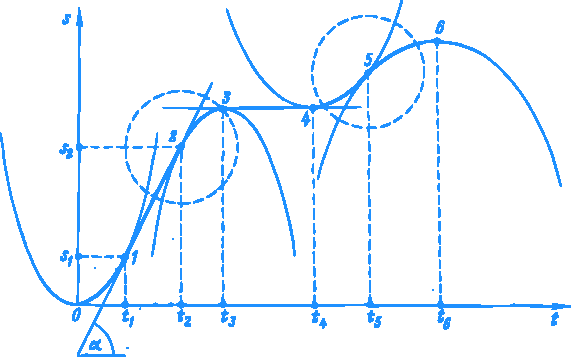
\includegraphics[width=\textwidth]{figures/fig-31.pdf}
\caption{Analysing the concept of instantaneous velocity.}
\label{fig-31}
\end{figure}

\athr Consider a graph of distance covered by a body plotted as a function of time, that is, the graph of the function $s = s (t)$. This graph is shown in \fig{fig-31} by a solid line. Note that in physics one typically uses the same symbol to denote both a function and its values (in this case we use the symbol $s$).

\rdr The figure also shows several thin lines.

\athr The thin lines (parabolas: and straight lines) are shown only to indicate how the graph of $s = s (t)$ was plotted. This graph is thus composed of ``pieces'' of parabolas and straight lines. For instance, for the time interval from 0 to $t_{1}$ the graph is represented by a ``piece'' of the extreme left-hand parabola (portion 0-1 of the graph). Please recall the formula for the distance covered in a uniformly accelerated motion with zero initial velocity.

\rdr This formula is 
\begin{equation}%
s (t) =\dfrac{at^{2}}{2}
\label{uniform-dist}
%eq-1
\end{equation}
 where $a$ is acceleration. 

\athr And the extreme left-hand parabola is the
graph of the function represented by your formula. 

\rdr So for the time interval from 0 to $t_{1}$ the body moves at a constant acceleration. 

\athr Exactly. 

\rdr I see. For the time interval from $t_{1}$ to $t_{2}$ the
body moves uniformly (portion 1-2 of the graph is a straight line); from $t_{2}$ to $t_{3}$ the body moves at a constant deceleration (the graph is an inverse parabola); from $t_{3}$ to $t_{4}$ the body is not moving at all; from $t_{4}$ to $t_{5}$ it moves at a constant acceleration, and from $t_{5}$ to $t_{6}$ it moves at a constant deceleration.

\athr Precisely so. Now let us consider the graph of the function $s (t)$ shown in \fig{fig-31} from a purely mathematical standpoint. Let us pose the following question: How strongly do the values of the function change in response
to the value of its argument $t$ in different portions of the graph?

\rdr In portion 3-4 the values of the function $s (t)$ do not change at all, while in other portions they do. A slower rate of change of the function is observed in the vicinity	of	points	0,	3,	4,	and	 6;	a	faster	rate of change is observed in the vicinity of points 1, 2, and 5. As a matter of fact, the rate of change is equally fast throughout portion 1-2.

\begin{figure}[!ht]%[13]{r}{0.5\textwidth}
\centering
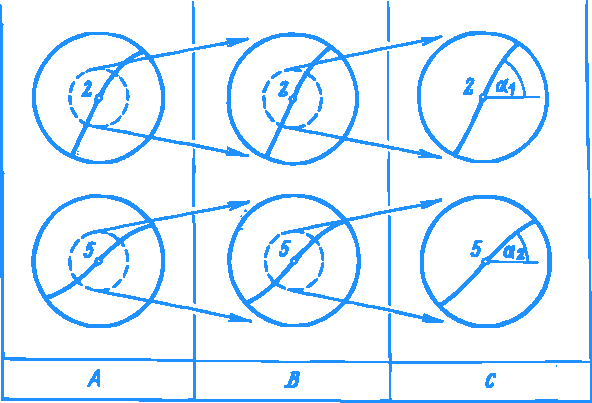
\includegraphics[width=\textwidth]{figures/fig-32.pdf}
\caption{Analysing the concept of instantaneous velocity mathematically.}
\label{fig-32}
\end{figure}

\athr You are a keen observer. And where do you think the rate of change is faster, at point 2 or at point 5? 

\rdr Of course, at point 2. Here the graph of the function has a much steeper slope than at point 5.	

\athr Let us turn to \fig{fig-32}. Here in column $A$ two portions of the graph of the function $s (t)$ are shown separately, namely, those in the vicinity of points 2 and 5 (in \fig{fig-31} these portions are identified by dash circles). In column $B$ the portions of the graph close to points 2 and 5 are shown again, but this time with a two-fold increase in scale. Column $C$ shows the result of another two-fold scale increase. Obviously, as the scale increases, the curvature of the graph $s (t)$ becomes less noticeable. We may say that the graph has a property of ``linearity on a small scale'', which enables us to consider the slope of the graph \emph{at a specific point}. In \fig{fig-32} (in column $C$) it is shown that the slope of the graph at point 2 is ($\alpha_{1}$ (the slope is measured relative to the $t$-axis), while the slope at point 5 is $\alpha_{2}$, and
clearly $\alpha_{2} < \alpha_{1}$.

Denote the slope of the curve $s (t)$ at the moment $t$ by $\alpha (t)$. Then $\tan \alpha (t)$ is said to be the rate of change of the function $s (t)$ at the moment $t$, or simply the instantaneous velocity.

\rdr But why tangent?

\athr You immediately come to it by considering portion 1-2 of the graph in \fig{fig-31}. This portion represents a uniform motion of the body, the rate of change of $s (t)$ being identical at all points. Obviously, it equals the
average velocity during the time interval $t_{2} -	t_{1}$ , which is 
\begin{equation*}%
\frac{s_{2}-s_{1}}{t_{2} - t_{1}} = \tan \alpha
\end{equation*}

\rdr In \fig{fig-32} you have demonstrated a ``straightening'' of the graph by increasing its scale. But this straightening is only \emph{approximate}. Why have you stopped at a mere four-fold scale increase?

\athr We can get rid of this approximation and formulate a more rigorous definition of a slope at a point. To be more specific, we consider a segment of the graph $s (t)$ close to point 5. In this segment we select an arbitrary point $B$ and draw a secant through points 5 and B (\fig{fig-33}). Next, on the same graph between points 5 and $B$ we select an arbitrary point $C$ and draw a new secant $5C$. Further, we select an arbitrary point $D$ in the segment between 5
and $C$ and draw a new secant $5D$. We may continue this process infinitely long and, as a result, we obtain a sequence of secants which converges to a certain straight line (line $5A$ in \fig{fig-33}). This straight line is said to be tangent to the curve at point 5. \emph{The slope of the tangent is said to be the slope of the graph at a given point.}
\begin{figure}[!ht]%[13]{r}{0.5\textwidth}
\centering
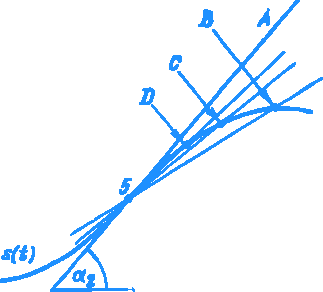
\includegraphics[width=0.5\textwidth]{figures/fig-33.pdf}
\caption{Analysing the concept of instantaneous velocity mathematically.}
\label{fig-33}
\end{figure}

\rdr If I understand you correctly we are now in a position to formulate strictly the answer to the question about the instantaneous velocity.

\athr Try to do it, then.

\rdr The instantaneous velocity of a body at a moment of time $t$ is the rate of change of $s (t)$ at the moment $t$. \emph{Numerically it is equal to the tangent of the slope of the tangent line to the graph of the function $s (t)$ at the moment $t$.}

\athr Very good. But you should have mentioned that $s(t)$ expresses the distance covered by the body as a function of time.

\rdr This is true, my definition of the instantaneous velocity is tied to the \emph{graph} of $s (t)$. What if the function $s (t)$ is not defined graphically?

\athr Anyway, a graph for $s (t)$ always exists. The only ``inconvenience'' in your definition is that it is necessary to take into account the scale of units on the coordinate axes. If the unit of time (on the $t$-axis) and the unit of length (on the $s$-axis) are represented by segments of identical length, the instantaneous velocity at time $t$ is
\begin{equation*}%
\tan \alpha (t) \, \dfrac{\text{unit of length}}{\text{unit of time}}
\end{equation*}
If, however, the segment representing one unit of length is $n$ times greater than the segment representing one unit of time, the instantaneous velocity is
\begin{equation*}%
\frac{1}{n} \, \tan \alpha (t) \, \dfrac{\text{unit of length}}{\text{unit of time}}
\end{equation*}
This ``inconvenience'', however, has no principal significance. But it is also possible to formulate a definition of the instantaneous velocity in a form free of graphic images.

Look at \fig{fig-34} which carries \fig{fig-33} one step further.
\begin{figure}[!ht]%[13]{r}{0.5\textwidth}
\centering
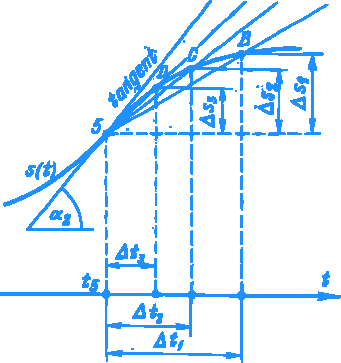
\includegraphics[width=0.5\textwidth]{figures/fig-34.pdf}
\caption{Analysing the concept of instantaneous velocity mathematically.}
\label{fig-34}
\end{figure}

\fig{fig-34} shows that the slope of the secant $5B$ is a ratio $\dfrac{\Delta s_{1}}{\Delta t_{1}}$. In other words, this is the average velocity for the time interval from $t_{5}$ to $t_{5} + \Delta t_{1}$. The slope of the secant $5C $is  $\dfrac{\Delta s_{2}}{\Delta t_{2}}$ that is, the average velocity for the time interval from  $t_{5}$ to  $t_{5} + \Delta t_{2} \,\, (\Delta t_{2} < \Delta t_{1})$. The slope of the secant $5D$ is $\dfrac{\Delta s_{3}}{\Delta t_{3}}$ that is, the average velocity for the time interval from $t_{5}$ to  $t_{5} + \Delta t_{3} \,\, (\Delta t_{3} < \Delta t_{2})$ , etc. Thus, a sequence of the secants converging to the tangent line (drawn at point 5 of the graph $s (t)$) corresponds to a sequence of the average velocities converging to the slope $\alpha_{2}$ of the tangent line, that is, to the value of the instantaneous velocity at the time moment $t_{5}$.

\rdr It comes out that the \emph{instantaneous velocity is the limit of a sequence of average velocities}.

\athr Precisely. The instantaneous velocity is in fact the limit of a sequence of average velocities, provided that the time interval over which the averaging is made tends to zero converging to the moment of time $t$ (viz., $t_{5}$ in \fig{fig-34}).

Now let us formulate the definition in a more rigorous manner. What we want to define is the instantaneous velocity of a body at a moment of time $t$. Consider an arbitrary time interval from $t$ to $t + \Delta t_{1}$. The distance covered by the body during this interval is $\Delta s_{1}$. The average velocity of the body during this time interval is
\begin{equation*}%
v_{\text{av}}  (t, \, \Delta t_{1}) = \frac{\Delta s_{1}}{\Delta t_{1}} 
\end{equation*}
Next we select a shorter time interval $\delta t_{2}$, from $t$ to $t + \Delta t_{2}, \,\, (\Delta t_{2} < \Delta t_{1})$, during which a distance $\Delta s_{2}$ is covered.  Consequently, the average velocity over $\Delta t_{2}$ is
\begin{equation*}%
v_{\text{av}}  (t, \, \Delta t_{2}) = \frac{\Delta s_{2}}{\Delta t_{2}} 
\end{equation*}
We continue this process of selecting shorter and shorter time intervals starting at the moment of time $t$. As a result, we obtain a sequence of the average velocities
\begin{equation*}%
v_{\text{av}}  (t, \, \Delta t_{1}), \,\, v_{\text{av}}  (t, \, \Delta t_{2}), \,\, v_{\text{av}}  (t, \, \Delta t_{3}), \ldots
\end{equation*}
The limit of this sequence for $ \Delta t \to 0$ is the instantaneous
velocity at the moment of time $t$:
\begin{equation}%
v(t) = \lim\limits_{ \Delta t \to 0} v_{\text{av}}  (t, \, \Delta t)
\label{instant-velocity}
%eq-2
\end{equation}
Taking into account that
\begin{equation*}%
v_{\text{av}}  (t, \, \Delta t) = \frac{s (t + \Delta t) - s(t)}{\Delta t}
\end{equation*}
we rewrite expression \eqref{instant-velocity} in the following form
\begin{equation}%
\boxed{
v(t) = \lim\limits_{ \Delta t \to 0} \frac{s (t + \Delta t) - s(t)}{\Delta t}}
\label{instant-velocity}
%eq-3
\end{equation}
As a result, we can formulate the following definition of the instantaneous velocity.
\begin{mytheo}{Definition}
The instantaneous velocity at a moment of time t is the limit of a sequence of average velocities over time intervals from $t$ to $t + \Delta t$ for $\Delta t \to 0$.
\end{mytheo}

\rdr Now I realize that instead of talking about a sufficiently small time interval $\Delta t $ (I am referring to our talk about the ratio $\dfrac{\Delta s }{\Delta t }$ at the beginning of the dialogue), the argument should have been based on the limit transition for $\Delta t \to 0$. In other words, the instantaneous velocity is not $\dfrac{\Delta s }{\Delta t }$  at a sufficiently small  $\Delta t$ but $\lim\limits_{\Delta t \to 0} \, \dfrac{\Delta s }{\Delta t }$ 

\athr Exactly. The definition formulated above for the instantaneous velocity not only exposes the gist of the concept but gives a rule for its calculation, provided that an analytical expression for $s (t)$ is known. Let us make such a calculation assuming that $s(t)$ is given by expression \eqref{uniform-dist}. 

\rdr We should substitute \eqref{uniform-dist} for \eqref{instant-velocity}. This gives
\begin{equation*}%
v(t) =  \lim\limits_{ \Delta t \to 0} \frac{\dfrac{a (t + \Delta t)^{2}}{2} - \dfrac{a t^{2}}{2}}{\Delta t}
\end{equation*}
\athr Go ahead. Remove the parentheses. 

\rdr This will give
\begin{equation*}%
\begin{split}
v(t) & =  \lim\limits_{ \Delta t \to 0} \frac{a (t^{2} + 2t \Delta t + \Delta t^{2} - t^{2})}{2 \Delta t}\\
& = \lim\limits_{ \Delta t \to 0} \left( at + \frac{\Delta t }{2} \right) \\
& = at
\end{split}
\end{equation*}
We have arrived at a familiar formula for the velocity of
uniformly accelerated motion with zero initial velocity:
\begin{equation}%
\boxed{
v(t) = at}
\label{uniform-velocity}
%eq-4
\end{equation}

\athr You are absolutely right. I must congratulate you: for the first time in your life you have carried the so-called operation of \emph{differentiation}. In other words, you have determined for a given function $s (t)$ its \emph{derivative}, that is, the function $v (t)$.

\rdr Does it mean that the instantaneous velocity is a derivative?

\athr Note that a derivative exists only \emph{with respect to} a known \emph{initial} function. If the initial function is $s (t)$ (path as a function of time), the derivative is the instantaneous velocity.

\begin{figure}[!ht]%[13]{r}{0.5\textwidth}
\centering
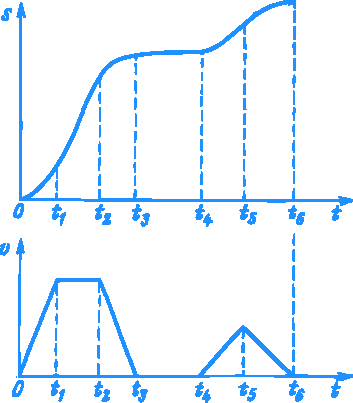
\includegraphics[width=0.6\textwidth]{figures/fig-35.pdf}
\caption{Comparing the graph of a function $s(t)$ and the graph of its rate
of change.}
\label{fig-35}
\end{figure}

Let us return now to the graph $s (t)$ shown in \fig{fig-31}. Our previous arguments and, in particular, relation \eqref{uniform-velocity}, allow us to transform the graph $s (t)$ into a graph of the derivative, that is, the function $v (t)$. A comparison of the two graphs is given in \fig{fig-35}. I recommend that you carefully analyze \fig{fig-35}, interpreting it as a comparison of the graph of a function $s (t)$ and the graph of its rate of change.}
% !TEX root = calculus.tex


\chapter{DERIVATIVE}
\label{derivative}

\athr The previous dialogue gave us an opportunity to introduce the concept of a \emph{derivative} for a specific example from physics (the instantaneous velocity of a body moving non-uniformly along a straight line). Now let us examine this concept from a purely mathematical viewpoint without assigning any physical meaning to the mathematical symbols used.

\begin{figure}[!ht]%[13]{r}{0.5\textwidth}
\centering
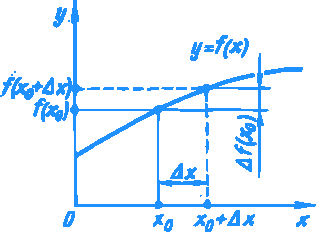
\includegraphics[width=0.6\textwidth]{figures/fig-36.pdf}
\caption{Examining concept of a derivative on an arbitrary function.}
\label{fig-36}
\end{figure}

\fig{fig-36} shows a graph of an arbitrary function $y = f (x)$. Let us select an arbitrary point $x= x_{0}$ from the domain of the function. In the subsequent argument this point is considered as \emph{fixed}. Now consider another point $x$ from the domain of the function and introduce a notation $\Delta x = x -	x_{0}$. The value $\Delta x$ is called the \emph{increment of the independent variable}. The increment is considered with respect to the fixed point $x_{0}$. Depending on the point $x$, the value of $\Delta x$ may. be larger or smaller, positive or negative.

Now let us examine a difference between the values of the function at points $x = x_{0} + \Delta x$ and $x = x_{0}$:
\begin{equation*}%
\Delta f (x_{0}) = f (x_{0} + \Delta x) - f(x_{0})
\end{equation*}
The difference  $\Delta f (x_{0})$ is said to be the \emph{increment of a function $f$ at a point $x_{0}$}. Since $x_{0}$ is fixed, $\Delta f (x_{0})$ should be considered as a function of a variable increment $\Delta x$ of the independent variable.

\rdr Then it is probably more logical to denote this function by $\Delta f (\Delta x)$, and not by $\Delta f (x_{0})$, isn't it?

\athr Probably, you are right. However, the accepted notation is $\Delta f (x_{0})$. Such a notation emphasized the fact that the increment of $f$ (in other words, the given function of $\Delta x$ is referred to point $x_{0}$.

With the concepts of the increment introduced, it is not difficult to evaluate the rate of change of $f$ close to $x_{0}$.


\rdr This rate should be described by the ratio $\dfrac{\Delta f(x_{0})}{\Delta x}$. For instance, if we compare $\Delta f(x_{0})$ with an increment of t at another point from the domain of the function (say, point $x = x_{1}$), we may obtain an inequality
\begin{equation*}%
\frac{\Delta f (x_{1})}{\Delta x} > \frac{\Delta f (x_{0})}{\Delta x} 
\end{equation*}
and therefore conclude that the rate of change of $f$ close to point $x_{1}$ is greater than that close to $x_{0}$.

\athr Please, be careful. You have not said anything about the vague increment $\Delta x$. If $\Delta x$ is too large, the inequality you have just mentioned may lead to a wrong conclusion. I shall make myself clearer by referring to
\fig{fig-37}. As you see,
\begin{equation*}%
\frac{\Delta f (x_{1})}{\Delta x} > \frac{\Delta f (x_{0})}{\Delta x} 
\end{equation*}
You must agree, however, that close to point $x_{0}$ the function changes much faster (the graph of the function has a steeper slope) than in the vicinity of $x_{1}$.

\begin{figure}[!ht]%[13]{r}{0.5\textwidth}
\centering
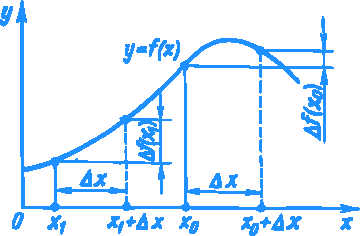
\includegraphics[width=0.6\textwidth]{figures/fig-37.pdf}
\caption{Examining concept of a derivative on an arbitrary function.}
\label{fig-37}
\end{figure}

\rdr It is necessary that the value of the increment $\Delta x$  be sufficiently small. The smaller is $\Delta x$ the more accurate is the information about the rate of change of the function close to the point under consideration.

\athr Well, we can do even better than this. We may, for example, consider the limit of the ratio $ \dfrac{\Delta f (x_{0})}{\Delta x} $ for $\Delta x \to 0$	(remember	the	previous dialogue). 

\rdr This limit will characterize the \emph{rate of change} of the function $f$ directly at $x =x_{0}$. 

\athr Exactly. Let us calculate the limit in detail:
\begin{equation}%
\lim\limits_{\Delta x \to 0}  \frac{\Delta f (x_{0})}{\Delta x} = \lim\limits_{\Delta x \to 0}   \frac{\Delta f (x+ x_{0}) - f (x_{0}) }{\Delta x}
% eq 1 of 09
\label{limit-in-detail}
\end{equation}
and examine first of all the mathematical nature of this limit.

\rdr Since point $x_{0}$ is fixed, it is evidently the limit of the ratio of two functions of  $\Delta x$  for  $\Delta x \to 0$ .

\athr Let us denote these functions by $F$ and $G$:
\begin{equation*}%
 F(\Delta x) = f( x_{0}+ \Delta x) - f(x_{0}),	\qquad G (\Delta x) = \Delta x
\end{equation*}


\rdr Limit \eqref{limit-in-detail} is then 
\begin{equation*}%
\lim\limits_{\Delta x \to 0} \frac{ F(\Delta x) }{ G(\Delta x) }
\end{equation*}
where $\lim\limits_{\Delta x \to 0}  F(\Delta x)=0$ and $\lim\limits_{\Delta x \to 0}  G(\Delta x)=0$. Hence, we have here a limit similar to that discussed at the end of Dialogue Seven, namely, a limit of the type $\dfrac{\infty}{\infty}$. 

\athr Right. This limit, that is, the limit of the type $\dfrac{\infty}{\infty}$ the main subject of this dialogue.

The primary requirement in this case is the \emph{existence} of the limit. It means that the function $f$ should be such that
\begin{equation*}%
\lim\limits_{\Delta x \to 0}F (\Delta x) = 0
\end{equation*}
The necessary condition for satisfying this equality is the \emph{continuity} of $f$ at $x =x_{0}$ But we shall discuss this problem later.


If the limit of the type  $ \dfrac{\infty}{\infty}$ (in other words, limit \eqref{limit-in-detail}) does exist, it is called ``the derivative of the function $f$ at point $x = x_{0}$ and usually denoted by $f'(x_{0})$.''

\begin{mytheo}{Definition}
The derivative of a function $f$ at a point $x_{0}$ (denoted by $f'(x_{0})$) is the limit of the ratio of an increment of the function $f$ at the point $x_{0}$ (denoted by  $\Delta f(x_{0})$) to an increment $\Delta x$ the independent variable for $\Delta x \to 0$:
\begin{equation*}%
f'(x_{0}) = \lim\limits_{\Delta x \to 0} \frac{\Delta f(x_{0})}{\Delta x}
\end{equation*}
or, in a more detailed notation,
\begin{equation}%
f'(x_{0}) = \lim\limits_{\Delta x \to 0} \frac{\Delta f(x_{0})}{\Delta x}
% eq 2 of 9
\label{derivative-defn}
\end{equation}
\end{mytheo}
Note that you are already familiar with the right-hand side of equation \eqref{derivative-defn} (cf. expression \eqref{instant-velocity} from the previous dialogue).

\rdr Actually the derivative of the function $f$ at point 0 is the limit of the function 
\begin{equation*}%
\frac{F}{G} =	\frac{ f (x_{0} + \Delta x) - f (x_{0})}{\Delta x}
\end{equation*}
at $ \Delta x = 0$. The independent variable of the function $\dfrac{F}{G}$
is the increment $\Delta x$. 

\athr You are quite right. However, in what follows you must use the definition of the derivative as formulated above. This definition does not involve the function $\dfrac{F}{G}$ of $\Delta x$ since this function plays, as you understand, only an auxiliary role. We should simply bear in mind that the phrase ``the limit of the ratio of an increment $\Delta f (x_{0})$ to an increment $\Delta x$ for $\Delta x \to 0$'' describes the limit of a function of $\Delta x$, i.e. the function $\dfrac{F}{G}$, which is considered at $\Delta x = 0$.

The derivative can be also interpreted \emph{in terms of geometry}.

\rdr Shall we do it by using again the tangent to the graph of a function?

\athr Yes, of course. Let us take the graph $y = f (x)$ (\fig{fig-38}), fixing a point $x = x_{0}$. Consider an increment $\Delta x_{1}$  of the argument; the corresponding increment of the function at point $ x_{0}$ is $\Delta f_{1} (x_{0})$. Denote the slope of the chord $AB_{1}$ by $\alpha_{1}$ it is readily apparent that 
\begin{equation*}%
\frac{\Delta f_{1}(x_{0})}{\Delta x_{1}}  = \tan \alpha_{1}
\end{equation*}

\begin{figure}[!ht]%[13]{r}{0.5\textwidth}
\centering
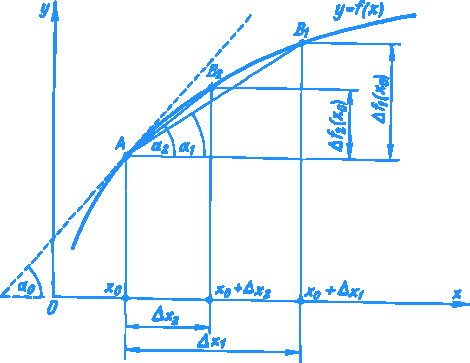
\includegraphics[width=0.8\textwidth]{figures/fig-38.pdf}
\caption{Examining concept of a derivative geometrically.}
\label{fig-38}
\end{figure}

Next take an increment $\Delta x_{1}$ (so that $\Delta x_{2}< \Delta x_{1}$). This increment corresponds to the increment $f_{2}(x_{0})$ of the function $f$ at point $x_{0}$. Denote the slope of the chord $AB_{2}$ by $\alpha_{2}$; it is similarly quite apparent that 
\begin{equation*}%
\frac{\Delta f_{2}(x_{0})}{\Delta x_{2}}  = \tan \alpha_{2}
\end{equation*}


Further, take an increment $\Delta x_{3}$ (so that $\Delta x_{3}< \Delta x_{2}$), and so on. As a result, we obtain an infinitesimal sequence of increments of the independent variable:
\begin{equation*}%
\Delta x_{1}, \, \Delta x_{2},  \,  \Delta x_{3},  \, \Delta x_{4},  \, \ldots \Delta x_{n},  \, \ldots
\end{equation*}
and the corresponding infinitesimal sequence of increments of the function at point $x_{0}$: 
\begin{equation*}%
\Delta f_{1} (x_{0}),  \, \Delta f_{2} (x_{0}),  \, \Delta f_{3} (x_{0}),  \, \Delta f_{4} (x_{0}),  \, \ldots \Delta f_{n} (x_{0}),  \, \ldots
\end{equation*}
This leads to a new sequence of the values of the tangent of the slopes of the chords $AB_{1}, AB_{2}, AB_{3}, \ldots AB_{n}, \ldots$. obtained as a sequence of the ratios of the two sequences given above
\begin{equation}%
\tan \alpha_{1},  \, \tan \alpha_{2},  \, \tan \alpha_{3},  \, \tan \alpha_{4},  \, \dots \tan \alpha_{n},   \, \ldots 
% eq 3 sec 9
\label{geom-defn-derivative}
\end{equation}
Both sequences $\Delta x_{n}$ and $\Delta f_{n} (x_{0})$ converge to zero. And what can be said about the convergence of the sequence ($\tan \alpha_{n}$) or, in other words, the sequence $\dfrac{\Delta f_{n} (x_{0})}{\Delta x_{n}}$?

\rdr Obviously, the sequence $\dfrac{\Delta f_{n} (x_{0})}{\Delta x_{n}}$ converges to $f' (x_{0})$. In other words, the limit of  $\dfrac{\Delta f_{n} (x_{0})}{\Delta x_{n}}$ is the derivative of $f$ at $x_{0}$. 

\athr What are the grounds for this conclusion? 

\rdr Why, isn't it self-evident? 

\athr Let me help you. Your conclusion is based
on \emph{Definition 2} of the limit of function at a point. Don't you think so?

\rdr Yes, I agree. Indeed, a certain number (in this case $f' (x_{0}$ is the limit of a function $\Phi (\Delta x)$ (in this case $\Phi = \dfrac{F}{G}$) at $\Delta x = 0$ if for any sequence $\Delta x_{n}$ convergent to zero the corresponding sequence $(\Phi (\Delta x_{n}))$ converges to this number. Sequence \eqref{geom-defn-derivative} is precisely the sequence $(\Phi (\Delta x_{n}))$ in our case.

\athr Correct. We have thus found that $\lim\limits_{n \to \infty} \tan \alpha_{n} = f' (x_{0})$. Now look at \fig{fig-38} and tell me which direction is the limit for the sequence composed of the chords  $AB_{1}, \, AB_{2}, \,  AB_{3},  \, \ldots AB_{n},  \, \ldots$? 

\rdr It is the direction of the \emph{tangent} to the graph $f (x)$ at point $x = x_{0}$.

\athr Correct. Denote the slope of the tangent line by $\alpha_{0}$. Thus
\begin{equation*}%
\lim\limits_{n \to \infty} \tan \alpha_{n} = \tan \alpha_{0}
\end{equation*}
Consequently,
\begin{equation*}%
f' (x_{0}) = \tan \alpha_{0}
\end{equation*}
We thus obtain the following geometrical interpretation of the derivative:
\begin{mytheo}{}
The derivative of a function $f$ at a point $x_{0}$ is defined by the slope of the tangent to the graph of the function $f$ at the point $x = x_{0}$.
\end{mytheo}

Note that the slope of the tangent is measured relative to the positive direction of the abscissa axis, so that the derivative of $f$ at point $x_{0}$ in \fig{fig-39} is positive (at this point $\tan \alpha_{0} > 0$), while at point $x_{0}$ the derivative of $f$ is negative $\tan \alpha_{0} < 0$).

\begin{figure}[!ht]%[13]{r}{0.5\textwidth}
\centering
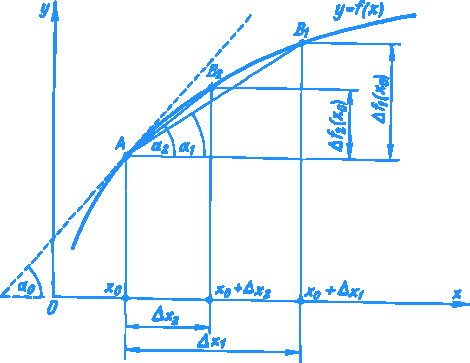
\includegraphics[width=0.8\textwidth]{figures/fig-38.pdf}
\caption{Examining concept of a derivative geometrically.}
\label{fig-39}
\end{figure}

But the geometrical interpretation of the derivative must not upstage the basic idea that
\begin{mytheo}{}
The derivative of a function $f$ at a point $x_{0}$ is the rate of change of $f$ at this point.
\end{mytheo}

In the previous dialogue we analyzed the function $s (t)$ describing the dependence of the distance covered by a body during the time $t$. In this case the derivative of $s (t)$ at a point $t = t_{0}$ is the \emph{velocity} of the body at the moment of time $t = t_{0}$. If, however, we take $v (t)$ as the initial function (the instantaneous velocity of a body as a function of time), the derivative at  $t = t_{0}$ will have the meaning of the acceleration of the body at  $t = t_{0}$. Indeed, \emph{acceleration} is the \emph{rate of change of the velocity} of a body.

\rdr Relation \eqref{derivative-defn} seems to allow a very descriptive (if somewhat simplified) interpretation of the derivative. We may say that
\begin{mytheo}{}
The derivative of a function $y = f (x)$ at a point $x = x_{0}$ shows how much steeper the change in $y$ is in comparison with the change in $x$ in the neighbourhood of $x = x_{0}$.
\end{mytheo}

\athr This interpretation of the derivative is quite justified, and it may be useful at times.

Getting back to the geometrical interpretation of the derivative, we should note that it immediately leads to the following rather important

\begin{mytheo}{Conclusions:}
\begin{enumerate}[label=\textsection]
\item The derivative of a function $f = \text{const}$ (the derivative of a constant) is zero at all the points.
\item The derivative of a junction $f = ax + b$ (where $a$ and $b$ are constants) is constant at all the points and equals $a$.
\item The derivative of a function $f = \sin x$ is zero at the points $x = + \pi n$ (at these points the tangent to the graph of the function is horizontal).
\end{enumerate}
\end{mytheo}

This ``list'' could, of course, be expanded.

Next I would like to attract your attention to the following: from the viewpoint of mathematics a derivative of a function must also be considered as a certain function.

\rdr But the derivative is a limit and, consequently, a \emph{number}!

\athr Let us clarify this. We have fixed a point $x = x_{0}$ and obtained for a function $f (x)$ at this point the number
\begin{equation*}%
\lim\limits_{\Delta x \to 0} \frac{\Delta f (x_{0})}{\Delta x}
\end{equation*}
For each point $x$ (from the domain of $f$) we have, in the general case, its own number
\begin{equation*}%
\lim\limits_{\Delta x \to 0} \frac{\Delta f (x)}{\Delta x}
\end{equation*}
\begin{mytheo}{}
This gives a mapping of a certain set of numbers $x$ onto a different set of numbers $\lim\limits_{\Delta x \to 0} \dfrac{\Delta f (x)}{\Delta x}$. The function which represents this mapping of one numerical set onto another is said to be the derivative and is denoted by $f'(x)$.
\end{mytheo}

\rdr I see. So far we have considered only one value of the function $f (x)$, namely, its value at the point $x = x_{0}$.

\athr I would like to remind you that in the previous dialogue we analyzed $v (t) $ which was the derivative of $s (t)$. The graphs of the two functions (i.e. the initial function $s (t)$ and its derivative $v (t)$) were even compared in \fig{fig-35}.

\rdr Now it is clear.

\athr I would like to make two remarks with regard to $f' (x)$.

\textcolor{IndianRed}{\textbf Note 1}. A function $f' (x)$ is obtained only by using a function  $f (x)$. Indeed,
\begin{equation}%
\boxed{
f' (x) = \lim\limits_{\Delta x \to 0} \frac{f (x + \Delta x) - f(x)}{\Delta x}}
\label{note-1-def}
%eq-4 of 9
\end{equation}
It is as if there is a certain operator (recall \hyperref[function]{Dialogue Four}) which generates $f' (x)$ at the output in response to $f (x)$ at the input. In other words, this operator, applied to the function $f (x)$, ``generates'' $f' (x)$. This operator is usually
denoted by $\dfrac{d}{dx}$. This notation should be interpreted as a single entity and not as a ratio (it reads: ``$d$ over $dx$''). 

Consider an ``image''
\begin{equation*}%
\frac{d}{dx} \boxed{1} = \boxed{2}. 
\end{equation*}
The squares in this
expression symbolize the familiar ``windows''. ``Window'' 1 is to input $f (x)$, while ``window'' 2 outputs $f' (x)$. Thus,
\begin{equation}%
\boxed{
\frac{d}{dx}  f (x) = f' (x)}
\label{note-1-def2}
%eq-5 of 9
\end{equation}

\begin{mytheo}{Definition:}
The operation of obtaining $f' (x)$ from $f (x)$ is said to be the differentiation of $f (x)$.
\end{mytheo}
The operator $\dfrac{d}{dx}$ performs this operation over $f (x)$ and is said to be the operator of differentiation.

\rdr But what exactly is $\dfrac{d}{dx}$ doing with $f (x)$? 

\athr It is exactly the operation prescribed by \eqref{note-1-def}.
We may say that $\dfrac{d}{dx}$ ``constructs'' the ratio 
\begin{equation*}%
\frac{(x + \Delta x) - f(x)}{ \Delta x}
\end{equation*}
from $f (x)$ and determines the limit of this ratio (regarded as a function of $\Delta x$) at $dx = 0$.

\rdr In other words, the operator $dx$ performs  a certain limit transition operation, doesn't it? 

\athr Certainly. The whole	differential	calculus (and with it, integral calculus) can be formulated in terms of certain limit transitions. 

\rdr Why should we introduce an operator $\dfrac{d}{dx}$ if it represents nothing else but the limit transition operation described by \eqref{note-1-def}?

\athr You have posed a very important question. The problem is that if we had formulated differential calculus in terms of limits, using the relations of type \eqref{note-1-def}, all books on calculus should have been increased in their volume several-fold and become hardly readable. The use of the relations of type \eqref{note-1-def2}, instead of \eqref{note-1-def}, makes it possible to avoid this.

\rdr But how can we use the relations of type \eqref{note-1-def2} \emph{without implicitly applying} the relations of type \eqref{note-1-def}?

\athr What is done is this. 

First, using \eqref{note-1-def}, we find the result of applying the operator $\dfrac{d}{dx}$ to a sum, product, and ratio of functions, and to composite
or inverse functions \emph{provided} that the result of applying the operator to the initial function (or functions) is \emph{known}. In other words, the first step is to establish the \emph{rules for the differentiation of functions}.

Second, using  \eqref{note-1-def}, we find out the result of applying $\dfrac{d}{dx}$ to some basic elementary functions (for instance, $y = x^{n}, \, y = \sin x, \,\, \text{and} \,\, y = \log x$).

After these two steps are completed you can practically forget about the relations of type \eqref{note-1-def}. \emph{In order to differentiate a function, it is sufficient to express the function via basic elementary functions (the derivatives of which were obtained earlier) and apply the rules for differentiation.}

\rdr Does it mean that the relations of type \eqref{note-1-def}
could be put aside after they have been used, first, for compiling a \emph{set of differentiation rules} and, second, for making a \emph{table of derivatives for basic elementary functions}?

\athr Yes, this is the procedure. Using the differentiation rules and the table of derivatives for some basic elementary functions you are in a position to forget about the relations of type \eqref{note-1-def} and are free to proceed further by using the ``language'' of the relations of type \eqref{note-1-def2}. A formal course of differential calculus could skip the analysis of limit transition operations, that is, the relations of type \eqref{note-1-def}. It is quite sufficient for a student to learn a set of differentiation rules and a table of derivatives of some functions.

\rdr I certainly prefer to be given the foundation.

\athr Our next dialogue will be devoted to a discussion of the programme of actions as outlined above. At the first step of the programme, the main rules for differentiation will be established on the basis of the relations of \eqref{note-1-def} and, in addition, the derivatives of three functions $y = x^{2}, \, y = \sin x, \, \, \text{and} \,\, y = \log_{a} x$ will be obtained. At the second step, we shall obtain (without reference to the relations of type \eqref{note-1-def}) the derivatives of the following functions: 

$y=x^{n}, \, y=x^{-n}, \, y= \sqrt{x}, \, y= \cos x, \, y= \tan x, \, y = \cot x, \, y = \arcsin x, \, y = \arccos x,\,  y= \arctan x, y = \arccot x, \,\, \text{and} \,\, y = a^{x}$.

\rdr I'll be looking forward to the next dialogue. By the way, you wanted to make one more remark about the derivative $f' (x)$.

\athr \textcolor{IndianRed}{Note 2} concerns the natural domain of a derivative. Let a set $D$ be the domain of $f (x)$. The question is whether $D$ is also the domain of $f' (x)$.

\rdr In any case, the domain of $f' (x)$ cannot be wider than the domain of $f (x)$ because in order to find $f' (x)$ we use $f (x)$.

\athr A carefully balanced answer, to be sure. The domain of $f' (x)$ is in the general case a subset of $D$. It is obtained from $D$ as a result of elimination of those points $x$ for which $\lim\limits_{\Delta x \to 0} \dfrac{\Delta f (x)}{\Delta x}$ does not exist. By the way, this subset is called the \emph{domain of differentiability} of $f (x)$. 

\rdr What are the \emph{conditions of differentiability} of $f(x)$ at any specific point $x$?

\athr Obviously, these conditions are identical to those of the existence of $\lim\limits_{\Delta x \to 0} \dfrac{\Delta f (x)}{\Delta x}$ at point $x$. We have
already observed that it is the limit of the type {\smaller $\dfrac{\infty}{\infty}$}, which necessitates that both the numerator and denominator tend to zero. It means that $f (x)$ must be continuous at $x$. The following theorem could be proved rigorously.

\begin{mytheo}{Theorem:}
The continuity of a function $f (x)$ at a point $x$ is a necessary condition for the existence of $f' (x)$ at $x$.
\end{mytheo}
However, we shall not give the proof of this theorem here. The simple qualitative arguments given above will suffice.

\rdr I wonder whether the continuity of a function is also a \emph{sufficient} condition for its differentiability.

\athr No, it is not. Consider, for example, the function $y = | \log x |$. It is sufficient only to look at its graph (\fig{fig-40}) to conclude that at $x = 1$ the tangent to the graph of the function is, strictly speaking, nonexistent (on approaching $x = 1$ from the left we have one tangent, viz., the straight line $AA$, while on approaching $x = 1$ from the right we have another tangent, viz., the straight line $BB$). It means that $y = | \log x |$ does not have a derivative at $x = 1$, although the function is continuous at this point.

\begin{figure}[!ht]%[13]{r}{0.5\textwidth}
\centering
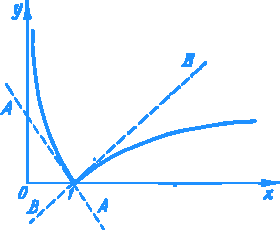
\includegraphics[width=0.6\textwidth]{figures/fig-40.pdf}
\caption{Examining the derivative of the function $y = | \log x |$.}
\label{fig-40}
\end{figure}


In conclusion, let us turn to one interesting property of differentiable functions. 

Let $f (x)$ be a differentiable function, and its increment $\Delta f$ at $x$ be related to the increment $\Delta x$ of the argument as follows:
\begin{equation}%
\Delta f= f' (x) dx +  \eta (\Delta x) \Delta x
\label{diff-func}
%6 of 9
\end{equation}
where $ \eta (\Delta x)$is a function of $ \Delta x$. 

By dividing both parts of \eqref{diff-func} by $\Delta x$, we obtain
\begin{equation*}%
\frac{\Delta f}{\Delta x} =f' (x) + \eta (\Delta x)
 \end{equation*}

Passing to a limit in both sides of the last equation for $\Delta x$ gives $\lim\limits_{\Delta x \to 0} \eta (\Delta x) =0$.

Consequently, $\eta (\Delta x)$ is an \emph{infinitesimal} (we use the same terminology as for numerical sequences, see Dialogue Three).

\begin{mytheo}{Conclusion:}
An increment $\Delta f$ of at a point $x$ of a function $f (x)$ differentiable at this point can be represented by two summands, namely, a summand proportional to the increment $\Delta x$ of the argument (this summand is $f' (x) \Delta x$) and a summand negligible in comparison with the first for sufficiently small $\Delta x$ (this summand is $\eta (\Delta x) \Delta x$, where  $\eta (\Delta x)$ is infinitesimal).
\end{mytheo}

\rdr It seems that this is a formulation of the property of ``linearity on a small scale'' that you mentioned in the previous dialogue (see \fig{fig-32}).

\athr Quite true. The main part of the increment of a differentiable function (a summand linear with respect to $\Delta x$) is called the \emph{differential} of the function.

% !TEX root = calculus.tex


\chapter{DIFFERENTIATION}
\label{differentiation}

\athr Now our aim is a practical realization of the programme outlined in the previous dialogue. This dialogue could be considered as a drill on the calculation of derivatives. We shall divide the talk into three parts.
\begin{enumerate}
\item Differentiation rules.

\item Differentiation of elementary functions	$y = x^{2},	\, y	= \sin x, \,\, \text{and} \,\, y = \log_{a} x$. 
\item Application of differentiation rules to different functions.
\end{enumerate}

Before the start I would like to remind you that the differentiation of a function $f (x)$ is defined as the operation of obtaining $f' (x)$ from $f (x)$. This operation is performed by using the operator of differentiation $\dfrac{d}{dx}$
\begin{equation*}%
\frac{d}{dx} f(x) = f'(x)
\end{equation*}


\section*{The Differentiation Rules}
\label{diff-rules}
% sec 1 of 10

\athr \textbf{Rule One.} We shall prove the following theorem:
\begin{mytheo}{Theorem}
The derivative of the sum of two functions equals the sum of their derivatives provided that they exist, i.e.
\begin{equation}%
\frac{d}{dx} \left[f(x) + g(x) \right] = \frac{d}{dx} f(x)  + \frac{d}{dx} g(x) 
\label{deriv-sum}
% eq 1 of 10
\end{equation}
\end{mytheo}

Denote $f (x) + g (x) =u (x)$. Then the theorem can be written as follows: $u' (x) = f' (x) + g' (x)$. Try to prove this theorem.

\rdr First I write
\begin{align*}%
f' (x) & =\lim\limits_{\Delta x \to 0} \frac{f (x + \Delta x) - f(x)}{ \Delta x} \\
g' (x) & = \lim\limits_{\Delta x \to 0} \frac{g (x + \Delta x) - g(x)}{ \Delta x} \\
u'(x) & = \lim\limits_{\Delta x \to 0} \frac{u (x + \Delta x) - u(x)}{ \Delta x} \\
& = \lim\limits_{\Delta x \to 0}  \frac{f (x + \Delta x) + g (x + \Delta x) - f(x) - g(x)}{ \Delta x} \\
\end{align*}

But I don't know what to do next. 

\athr We shall repeat your writing but drop the limit signs:
\begin{align*}%
\frac{\Delta u(x)}{ \Delta x} & =  \frac{f (x + \Delta x) + g (x + \Delta x) - f(x) - g(x)}{ \Delta x} \\
& =  \frac{f (x + \Delta x)  - f(x) }{ \Delta x} +  \frac{g (x + \Delta x) - g(x)}{ \Delta x} \\
& = \frac{\Delta f(x)}{ \Delta x}  + \frac{\Delta g(x)}{ \Delta x} 
\end{align*}
This gives
\begin{equation*}%
\frac{\Delta u(x)}{ \Delta x}  = \frac{\Delta f(x)}{ \Delta x}  + \frac{\Delta g(x)}{ \Delta x} 
\end{equation*}

\rdr I see. Next we use the well-known theorem on the limit of the sum of functions, and the proof is complete. 

\athr Quite correct. \textbf{Rule Two.} Let us prove the
next theorem:
\begin{mytheo}{Theorem}
 A constant multiplier is factored out of the derivative, that is
\begin{equation}%
\frac{d}{dx} \left[a \, f(x) \right] =a \, \frac{d}{dx} f(x)
\label{deriv-const}
% eq 2 of 10
\end{equation}
\end{mytheo}
The theorem is immediately proved if we use the following obvious equality
\begin{equation*}%
\frac{\Delta \left[a \, f(x) \right]}{ \Delta x}  = a \, \frac{\Delta f(x)}{ \Delta x} 
\end{equation*}

\textbf{Rule Three.} Now we shall consider the theorem on the derivative of the product of two functions.
\begin{mytheo}{Theorem}
The derivative of a function $u (x) = f (x) \, \, g (x)$ is calculated
by using the following formula:
\begin{equation}%
 u' (x) = f' (x) \, g (x) + f (x) \, g' (x)
 \label{deriv-prod}
% eq 3 of 10
\end{equation}
provided that the derivatives $f' (x)$ and $g' (x)$ exist. 
\end{mytheo}
Formula \eqref{deriv-prod} is called the \emph{Leibnitz formula}. Another expression for the same formula is:
\begin{equation*}%
\frac{d}{dx} (f \, g) = g \, \frac{d}{dx} f  +  f \, \frac{d}{dx} g 
\end{equation*}
\rdr Apparently, as in the proof of the first theorem, we must express $\dfrac{\Delta u (x)}{\Delta x}$ through $\dfrac{\Delta f (x)}{\Delta x}$ and $\dfrac{\Delta g (x)}{\Delta x}$. But how to do it? 

\athr The simplest way is
\begin{align*}%
u + \Delta u & = (f + \Delta f) (g +  \Delta g)  \\
& = fg + g \Delta f + f \Delta g + \Delta f \Delta g
\end{align*}
Hence,
\begin{equation*}%
\Delta u = g \Delta f + f \Delta g + \Delta f \Delta g
\end{equation*}
 consequently,
\begin{equation*}%
\frac{\Delta u (x)}{\Delta x} = g(x) \frac{\Delta f (x)}{
\Delta x} +  f(x) \frac{\Delta g (x)}{\Delta x} +   \frac{\Delta f (x)}{
\Delta x} \Delta g(x)
\end{equation*}
 
 Now we find the limit for $\Delta x \to 0$. Notice that neither $g (x)$ nor $f (x)$ depends on $\Delta x $, and $\Delta g (x)$ tends to zero. As a result,
 \begin{equation*}%
\lim\limits_{\Delta x \to 0 } \frac{\Delta u (x)}{\Delta x} = \lim\limits_{\Delta x \to 0 } g(x) \frac{\Delta f (x)}{\Delta x} + \lim\limits_{\Delta x \to 0 } f(x) \frac{\Delta g (x)}{\Delta x}
\end{equation*}
  The theorem is thus proved. 
 
 \textbf{Rule Four.} The next theorem is related to the derivative
of the ratio of two functions. 
\begin{mytheo}{Theorem}
The derivative of a function $u (x) = \dfrac{f(x}{g(x)}$ is: 
\begin{equation}%
u' (x) = \frac{f'(x) g(x) - f(x) g'(x)}{g^{2} (x)}
 \label{deriv-div}
% eq 4 of 10
\end{equation}
provided that the derivatives $f' (x)$ and $g' (x)$ exist, and that $g (x) \neq 0$.
\end{mytheo}
It can be written in a different form:
 \begin{equation*}%
 \ddx \left(\dfrac{f}{g} \right) =\dfrac{g \ddx f - f \ddx g}{g^{2}}
\end{equation*} 
Try to prove this theorem.
 
\rdr I shall proceed by analogy with the preceding proof. I can write
Hence,
 \begin{align*}%
\Delta u & = \dfrac{f + \Delta f}{g + \Delta g} - \dfrac{f}{g} \\
& = \dfrac{g \dfrac{\Delta f}{\Delta x} - f  \dfrac{\Delta g}{\Delta x} }{g^{2} + g \Delta g}
\end{align*} 
 This yields,
 \begin{equation*}%
\frac{\Delta u}{\Delta x} = \dfrac{g \dfrac{\Delta f}{\Delta x} - f  \dfrac{\Delta g}{\Delta x} }{g^{2} + g \Delta g}
\end{equation*} 


Passing then to the limit for $\Delta x \to 0$, I take into account that neither $g$ nor $f$ depend on $\Delta x$, and that $\Delta g$ also tends to zero. Using the known theorems on the limit of the product and the sum of functions, we obtain
\begin{align*}%
\lim\limits_{\Delta x \to 0} \frac{\Delta u}{\Delta x} & = \lim\limits_{\Delta x \to 0} \left(\dfrac{ 1 }{g^{2} + g \Delta g}  \right) \,\, \lim\limits_{\Delta x \to 0} \left( g \dfrac{\Delta f}{\Delta x}  - f \dfrac{\Delta g}{\Delta x}  \right) \\
& = \frac{1}{g^{2}} \left( g \lim\limits_{\Delta x \to 0} \frac{\Delta f}{\Delta x} - 
f \lim\limits_{\Delta x \to 0} \frac{\Delta g}{\Delta x} \right)
\end{align*}
This completes the proof. 

\athr Very good. Now we shall discuss the, problem
of the differentiation of a \emph{composite function} (for composite functions, see \hyperref[more-on-function]{Dialogue Five}. Let $w = h (x)$ be a composite function, and $h (x) = g [f (x)]$. This composite function is the composition of two functions $w =	g (y)$ and $y  = f (x)$.

I remind you that the derivative $f' (x)$ indicates how faster $y$ charges compared to $x$ and the derivative $g' (y)$ indicates how faster $w$ changes compared to $y$.  Consequently, the product $g' (y) f' (x)$ must indicate how faster $w$ changes compared to $x$, i.e. it equals the derivative $h' (x)$.

\textbf{Rule Five.} Thus we arrive at the differentiation rule for
composite functions.
\begin{mytheo}{Theorem}
The derivative of a composite function $h (x) = g [f (x)]$ is:
\begin{equation}%
h' (x) = g' (y) \, f' (x)
 \label{deriv-comp}
% eq 5 of 10
\end{equation}
\end{mytheo}

\rdr We have arrived at this rule using very simple arguments. I wonder whether they can be regarded as a proof of the rule.

\athr No, of course not. Therefore I am going to give the proof of the differentiation rule for composite functions.

Let the independent variable $x$ have an increment $\Delta x$ such that $x + \Delta x$ belongs to the domain of $f (x)$. Then the variable $y$ will have an increment $\Delta y = f (x + \Delta x) - f (x)$, while the variable $w$ will have an increment $\Delta w = g (y + \Delta y) - g (y)$. Since the derivative $g' (y)$ exists.
the increment $\Delta w$ can be expressed as follows
\begin{equation*}%
\Delta w = g'(y) \Delta y + \eta \Delta y
\end{equation*}
where $\eta \to 0$ for $\Delta y \to 0$ (see expression (6) from the previous dialogue). 

Dividing both sides of the equation by $\Delta x$,	 we obtain
\begin{equation*}%
\frac{\Delta w}{\Delta x} = g'(y) \frac{\Delta y}{\Delta x} + \eta \frac{\Delta y}{\Delta x}
\end{equation*}
Next we pass to the limit for $\Delta x \to 0$
\begin{equation*}%
\lim\limits_{\Delta x \to 0} \frac{\Delta w}{\Delta x} = g'(y) \lim\limits_{\Delta x \to 0} \frac{\Delta y}{\Delta x} + \lim\limits_{\Delta x \to 0} \left( \eta \frac{\Delta y}{\Delta x} \right)
\end{equation*}
Since $\lim\limits_{\Delta x \to 0} \frac{\Delta w}{\Delta x} = h' (x)$ and $\lim\limits_{\Delta x \to 0} \frac{\Delta y}{\Delta x} = f'(x)$, we have
\begin{equation*}%
h'(x) = g'(y) \,\, f'(x) + f'(x) \lim\limits_{\Delta  x \to 0} \eta 
\end{equation*}
And since $\Delta y \to 0$ for  $\Delta x \to 0$, 
\begin{equation*}%
\lim\limits_{\Delta  x \to 0} \eta = \lim\limits_{\Delta  y \to 0} \eta = 0
\end{equation*}

Hence we arrive at \eqref{deriv-comp}, namely, at the rule for the differentiation of composite functions.

\textbf{Rule Six.} Finally, I shall give (without proof) the rule for the differentiation of inverse functions.

\begin{mytheo}{Theorem}
If a derivative $y' (x)$ of an initial monotonic function $y (x)$ exists and is not equal to zero, the derivative of the inverse junction $x (y)$ is calculated by the formula:
\begin{equation}%
x' (y) = \frac{1}{ y' (x)}
 \label{deriv-comp}
% eq 6 of 10
\end{equation}
\end{mytheo}

\rdr It seems that this formula can be easily obtained if we make use of the geometrical interpretation of the derivative. Really, consider the graph of a monotonic function $y (x)$ (\fig{fig-41}); its derivative at point $x_{0}$ is $\tan \alpha$. The same curve can, obviously, be regarded as the graph of the inverse function $x (y)$, with $y$ considered as the independent variable instead of $x$, and $x$ considered as the dependent variable instead of $y$. But the derivative of the inverse function at point $y_{0}$ is $\tan \beta$ (see the figure). 
\begin{figure}[!ht]%[13]{r}{0.5\textwidth}
\centering
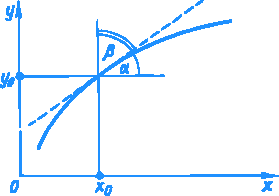
\includegraphics[width=0.6\textwidth]{figures/fig-41.pdf}
\caption{Derivative of a function and its inverse.}
\label{fig-41}
\end{figure}
Since $\alpha + \beta = \dfrac{\pi}{2}$ we have
\begin{equation*}%
\tan \beta = \frac{1}{\tan \alpha}
\end{equation*}

This gives the above-cited differentiation rule for inverse functions.

\athr I must admit that although your line of reasoning is not a rigorous mathematical proof, it is an example of an effective application of geometrical concepts.
\section*{The Differentiation of Functions \\
$y = x^{2}, \, y= \sin x, \, \, \text{and} \,\, y = \log_{a} x$}

\athr Using \eqref{note-1-def} from the previous dialogue, calculate the derivatives of the three indicated functions. Start with $y = x^{2}$. Go ahead.

\rdr I write
\begin{equation*}%
y + \Delta y = (x + \Delta x)^{2} = x^{2} + 2x	\Delta x + \Delta x^{2}
\end{equation*}
Hence, 
\begin{equation*}%
\Delta y =  2x	\Delta x + \Delta x^{2}
\end{equation*}
Consequently,
\begin{equation*}%
\frac{\Delta y}{\Delta x} =  2x	 + \Delta x
\end{equation*}
Further we pass to the limit for $\Delta x \to 0$
\begin{equation*}%
\lim\limits_{\Delta x \to 0} \frac{\Delta y (x)}{\Delta x} =  2x	
\end{equation*}
Therefore,
\begin{equation*}%
y' (x) = 2x
\end{equation*}

\athr You have thus obtained the result of applying the operator $\ddx$ to the function $y = x^{2}$:
\begin{equation}%
\boxed{
\ddx x^{2} = 2x}
\label{deriv-quad}
% eq 7 of 10
\end{equation}

We observe that for a quadratic function  $y = x^{2}$ at the input of the operator $\ddx$ we obtain a linear function $y = 2x$ at the output. 

Now try to differentiate the function $y = \sin x$. 

\rdr I shall write
\begin{equation*}%
y + \Delta y = \sin(x + \Delta x)^{2} = \sin x \cos \Delta x + \cos x \sin \Delta x 
\end{equation*}
Hence,
\begin{equation*}%
\Delta y = \sin x \cos \Delta x + \cos x \sin \Delta x - \sin x
\end{equation*}

\athr You had better use here the formula for the difference between two sines, not the formula for the sine of the sum. Represent $\Delta y$ in the form
\begin{equation*}%
\Delta y =  \sin(x + \Delta x) - \sin x = 2 \sin \frac{\Delta x}{2} \cos \left( x + \frac{\Delta x}{2} \right)
\end{equation*}
Next we obtain
\begin{equation*}%
\frac{\Delta x}{\Delta y} = \dfrac{ \sin \frac{\Delta x}{2}}{\frac{\Delta x}{2}} \cos \left( x + \frac{\Delta x}{2} \right)
\end{equation*}

In taking the limit for $\Delta x \to 0$, recall a result obtained in Dialogue Seven:
\begin{equation*}%
\lmts{\Delta x}{0} \frac{\sin \Delta x}{\Delta x} =1 
\end{equation*}

\rdr Yes, I see. Therefore,
\begin{align*}%
\lmts{\Delta x}{0} \frac{\Delta x}{\Delta y} & = \lmts{\Delta x}{0} \dfrac{ \sin \frac{\Delta x}{2}}{\frac{\Delta x}{2}} \lmts{\Delta x}{0} \cos \left( x + \frac{\Delta x}{2} \right) \\
& = \lmts{\Delta x}{0} \cos \left( x + \frac{\Delta x}{2} \right) \\
& = \cos x
\end{align*}

\athr The operator $\ddx$ applied to the function $y = \sin x$ thus generates the function $y = \cos x$:
\begin{equation}%
\boxed{ \ddx \sin x = \cos x}
\label{deriv-sin}
% eq 8 of 10
\end{equation}
Now we have to differentiate the function $y = \log_{a} x$. This time, however, we should start with a discussion of the transcendental number $e$ (which is usually called the ``base of natural or Napierian logarithms''). The number $e$ may be defined as the limit of a numerical sequence
\begin{equation}%
e  = \lmts{n}{\infty} \left( 1 + \frac{1}{n} \right)^{n}
\label{e-defn}
% eq 9 of 10
\end{equation}
The approximate value of e is: $e = \num{2.7182818284590}\ldots$
Using \eqref{e-defn}, we can show that $e$ is also the limit of $y = (1 + x)^{\dfrac{1}{x}}$ for $x$ tending to zero 
\begin{equation}%
\boxed{e  = \lmts{x}{0} \left( 1 + x \right)^{\dfrac{1}{x}}}
\label{e-defn2}
% eq 10 of 10
\end{equation}
We shall omit the proof of \eqref{e-defn2}. 

\rdr It seems that \eqref{e-defn2} follows logically from \eqref{e-defn}. 

\athr Far from it. Don't forget that in \eqref{e-defn} we deal
with the limit of a numerical sequence, while in \eqref{e-defn2} with the limit of a function at a point. While $n$ are integers, $x$ belongs to the real line (with the exception of $x = 0$). Therefore, the transition from \eqref{e-defn} to \eqref{e-defn2} requires a good deal of time and space.

Now turn to the differentiation of $y = \log_{a} x$. Follow the line adopted above. 

Start.

\rdr Obviously,
\begin{equation*}%
y + \Delta y = \\og_{a} (x+ \Delta x)
\end{equation*}
Hence,
\begin{align*}%
\Delta y & = \log_{a} (x+ \Delta x) -  \log_{a} x\\
& = \log_{a} \frac{x+ \Delta x}{ \Delta x}
\end{align*}
and, consequently,
\begin{equation*}%
\frac{\Delta x}{\Delta y} = \dfrac{ 1}{\Delta x} \log_{a} \frac{x + \Delta x}{x}
\end{equation*}
At this point I would have to find the limit for $\Delta x \to 0$. 

\athr I shall give you a hand here. We can rewrite
\begin{align*}%
\frac{\Delta x}{\Delta y} & = \log_{a} \left( \frac{x + \Delta x}{x} \right)^{\dfrac{1}{\Delta x}} \\
& =  \log_{a} \left( 1 + \frac{\Delta x}{x}  \right)^{\dfrac{x}{\Delta x} \cdot \dfrac{1}{x}} \\
& = \frac{1}{x} \log_{a} \left( 1 + \frac{\Delta x}{x} \right)^{\dfrac{ x}{\Delta x}}
\end{align*}

\rdr I see. This gives
\begin{equation*}%
\frac{\Delta x}{\Delta y}  = \frac{1}{x} \log_{a} \left( 1 + \frac{\Delta x}{x} \right)^{\dfrac{ x}{\Delta x}}
\end{equation*}
To find the limit for $\Delta x \to 0$, we use \eqref{e-defn2}. As a result 
\begin{align*}%
\lmts{\Delta x}{0} \frac{\Delta x}{\Delta y} & = \frac{1}{x} \lmts{\Delta x}{0}  \log_{a} \left( \frac{x + \Delta x}{x} \right)^{\dfrac{x}{\Delta x}} \\
& =  \frac{1}{x}  \log_{a} e \\
& =  \frac{1}{x} \cdot \frac{1}{\ln a}
\end{align*}
(symbol $\ln$ is the standard notation for the \emph{natural logarithm}).
 
\athr We have thus found that the operator $\ddx$ applied to the function $y = \log_{a} x$ gives $ y =  \dfrac{1}{x} \cdot \dfrac{1}{\ln a}$:
\begin{equation}%
\boxed{\ddx \log_{a} x  = \frac{1}{x} \cdot \frac{1}{\ln a}}
\label{deriv-log}
% eq 11 of 10
\end{equation}
Notice that the natural domain of the function $y =  \dfrac{1}{x} \cdot \dfrac{1}{\ln a}$ in \eqref{deriv-log} $] 0, \, \infty [$.

We can sum up our conclusions now. 
 
Using relation \eqref{note-1-def} from Dialogue Nine, first, we have established the six differentiation rules and, second, we have differentiated three functions. The results are summarized in \hyperref[diff-rules]{Table} on the next page, and \fig{fig-42} graphically represents the
result of the action of the operator $\ddx$ on the three selected
functions. The left-hand column in the figure lists the graphs of the three functions $f (x)$, and the right-hand column shows the graphs of the corresponding derivatives $f' (x)$.	


In what follows we shall not use formulas of type \eqref{note-1-def} from Dialogue Nine, that is, we shall not operate in terms of limit transitions. Using the results obtained above, we shall find the derivatives for a number of elementary functions without calculating the relevant limits.
\newpage 
\vspace*{1cm}

\begin{center}
\textcolor{DodgerBlue}{\textbf{The Differentiation Rules}}\\[30pt]
%{\smaller
\begin{tcolorbox}[colback=white,colframe=DodgerBlue]
%\boxed{
\begin{tabular}{p{5cm}>{\color{IndianRed}}l}
%\toprule
\textbf{Rule 1:} the differentiation of the sum of functions   & $\dfrac{d}{dx}(f + g) =  \dfrac{d}{dx}f + \dfrac{d}{dx} g $ \\
 \arrayrulecolor{DodgerBlue}\midrule
\textbf{Rule 2:} the differentiation of the function with constant term & $\ddx(af) = a \ddx f$ ($a$ = constant)\\
\midrule
\textbf{Rule 3:} the differentiation of the product of functions & $\ddx(fg) = f \ddx g + g \ddx f$\\
\midrule
\textbf{Rule 4:} the differentiation of the ratio of functions & $\ddx \dfrac{f}{g} = \dfrac{g \ddx f - f \ddx g }{g^{2}}$\\
\midrule
\textbf{Rule 5:} the differentiation of composite functions & $\ddx g[f(x)] = \left( \dfrac{d}{df} g(f) \right) \ddx f(x)$ \\
\midrule
\textbf{Rule 6:} the differentiation of inverse functions & $\dfrac{d}{dy} x(y) = \dfrac{1}{\ddx y(x)}$ 
%\bottomrule
\label{diff-rules}
\end{tabular}
%}
\end{tcolorbox}
\end{center}

\newpage


\begin{figure}[!ht]%[13]{r}{0.5\textwidth}
\centering
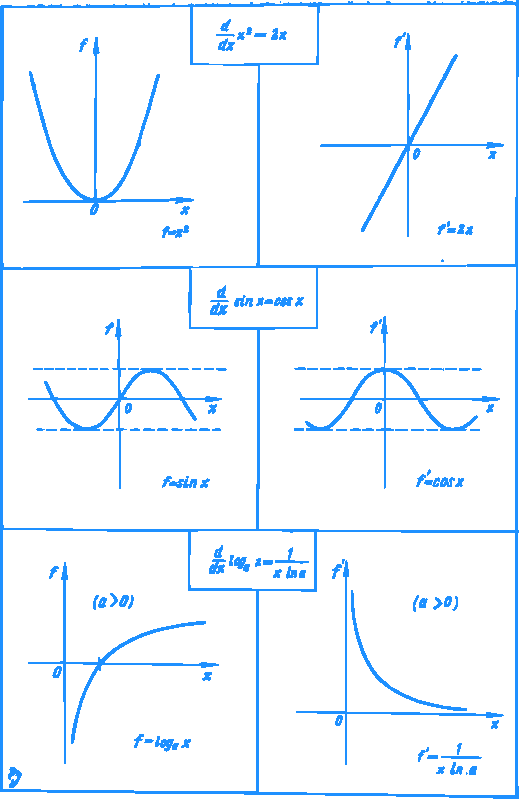
\includegraphics[width=.9\textwidth]{figures/fig-42.pdf}
\caption{Graphs of some basic functions and their derivatives.}
\label{fig-42}
\end{figure}


\section*{The Application of the Differentiation Rules to Different Functions}
\label{sec-3-9}

\athr As a first example, consider the function $y =x^{n}$. Prove that differentiation gives $y = n x^{n - 1}$ , that is,
\begin{equation}%
\boxed{\ddx x^{n}  = n x^{n-1}}
\label{deriv-power}
% eq 12 of 10
\end{equation}
Prove this proposition by using the \emph{method of mathematical induction}.

\rdr For $n = 2$ formula \eqref{deriv-power} holds and yields \eqref{deriv-quad}. Assume now that \eqref{deriv-power} holds for $n = m$. We have to prove that it is also true for $n = m +1$. We write $x^{m+1} = x^{m}\, x$ and use the \emph{Leibnitz formula} (\textbf{Rule Three}):
\begin{equation*}%
\ddx (x^{m}x) = x \ddx x^{m} + x^{m} \ddx x
\end{equation*}
Since $\ddx x = 1$ and according to the assumption $\ddx x^{m} = m x^{m-1}$, we obtain 
\begin{equation*}%
\ddx x^{m+1} = m x x^{m-1} + x^{m} = (m+1) x^{m}
\end{equation*}
The proof is completed. 

\athr The next example is the function $y = x^{-n}$.
Differentiate this function using \textbf{Rule Four} and \eqref{deriv-power}.


\rdr This is simple. Applying \textbf{Rule Four}, we obtain
\begin{equation*}%
\ddx \left( \frac{1}{x^{n}} \right) = \dfrac{-\ddx x^{n}}{x^{2n}}
\end{equation*}
By virtue of \eqref{deriv-power},
\begin{equation}%
\boxed{\ddx x^{-n}  = -n x^{-(n+1)}}
\label{deriv-power-neg}
% eq 13 of 10
\end{equation}
\athr One particular result that follows from \eqref{deriv-power-neg} is
\begin{equation}%
\boxed{\ddx \left( \frac{1}{x} \right)  = - \frac{1}{x^{2}}}
\label{deriv-power-neg}
% eq 14 of 10
\end{equation}
The next example is the function $y = \sqrt{x}$.

\rdr Here I shall use \textbf{Rule Six} (the differentiation rule for inverse functions). The inverse function involved is $x =y^{2}$. Its derivative is given by \eqref{deriv-quad}. As a result,
\begin{equation*}%
\ddx \sqrt{x} = \dfrac{1}{\ddx y^{2}} = \dfrac{1}{2y} = \dfrac{1}{2\sqrt{x}}
\end{equation*}
Thus
\begin{equation}%
\boxed{\ddx  \sqrt{x} = \dfrac{1}{2\sqrt{x}}}
\label{deriv-power-neg}
% eq 15 of 10
\end{equation}


\athr Now we can pass to the \emph{trigonometric} functions. Consider the function $y = \cos x$.

\rdr I propose to use \eqref{deriv-sin} and the identity $\sin^{2} x +  \cos^{2} = 1$. By differentiating both sides of the identity and using \textbf{Rule One}, we obtain
\begin{equation*}%
\ddx \sin^{2} x + \ddx \cos^{2} x = 0
\end{equation*}
Next, by applying \textbf{Rule Five} (the differentiation rule for composite functions) in conjunction with \eqref{deriv-quad}, we find
\begin{equation*}%
2 \sin x \ddx \sin x + 2 \cos x \ddx \cos x = 0
\end{equation*}
From \eqref{deriv-sin}, $\ddx \sin x= \cos x$ so that
\begin{equation*}%
\ddx \cos x = - \sin x 
\end{equation*}
\athr That is correct, although the result can be obtained in a simpler way. Better use the identity $\cos x = \sin \left(\dfrac{\pi}{2} -x \right)$. Further, applying \textbf{Rule Five}, we obtain
\begin{equation*}%
\ddx  \sin \left(\dfrac{\pi}{2} -x \right) = \left(\dfrac{d}{dy} \sin y \right) \ddx  \left(\dfrac{\pi}{2} -x \right)
\end{equation*}
(here  $y = \dfrac{\pi}{2} -x$)

Making use of \eqref{deriv-sin}, we find
\begin{equation*}%
\ddx  \sin \left(\dfrac{\pi}{2} -x \right) = - \dfrac{d}{dy} \sin y = - \cos y = - \sin x
\end{equation*}
Using now the suggested identity, we arrive at the final result:
\begin{equation}%
\boxed{\ddx  \sin x = - \cos x }
\label{deriv-sin}
% eq 16 of 10
\end{equation}

\rdr The operation of differentiation thus ``turns'' the sine into the cosine and, vice versa, that is, the cosine in to	 the sine.

\begin{figure}[!ht]%[13]{r}{0.5\textwidth}
\centering
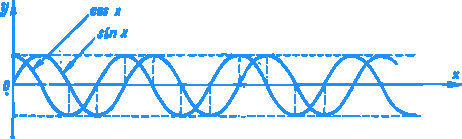
\includegraphics[width=\textwidth]{figures/fig-43.pdf}
\caption{Graphs of the sine and cosine functions.}
\label{fig-43}
\end{figure}

\athr. Yes, it does. But in the last case the sign changes too, that is, the cosine is transformed into the sine with a negative sign. If you plot the graphs of $\sin x$ and $\cos x$ in the same system of coordinates (\fig{fig-43}), you will find that at points $x$ where one of the functions reaches maximum or minimum (takes the value 1 or -1) the other function vanishes. It is readily apparent that this fact has
direct relation to your remark. If, for example, at a certain point $x$ the function $\sin x$ assumes its maximum value, the tangent to its graph at the same point will, obviously, be horizontal. 

Consequently, the derivative of the function (i.e, $\cos x$) must vanish at this point. I recommend that you carefully analyze \fig{fig-43}. In particular, follow the correspondence between the slope of the tangent to the graph of the function drawn at different points and the sign of the derivative at the same points.

Now turn to the next example, the function $y = \tan x$. Difierentiate this function using the results of the differentiation of $\sin x$ and $\cos x$ and applying \textbf{Rule Four}.

\rdr This will be easy:
\begin{align*}%
\ddx \left( \dfrac{\sin x}{\cos x} \right) & = \frac{\cos x \ddx \sin x - \sin x \ddx \cos x}{\cos^{2} x} \\
& = \frac{\cos^{2} x + \sin^{2} x}{\cos^{2} x} \\
& = \frac{1}{\cos^{2} x}
\end{align*}
Finally,
\begin{equation}%
\boxed{\ddx  \tan x = \frac{1}{ \cos^{2} x} }
\label{deriv-tan}
% eq 17 of 10
\end{equation}

\athr The result for $y = \cot x$ can be obtained similarly:
\begin{equation}%
\boxed{\ddx  \cot x = - \frac{1}{ \sin^{2} x} }
\label{deriv-tan}
% eq 18 of 10
\end{equation}
In order to differentiate $y = \arcsin x$, we use \textbf{Rule Six}
\begin{align*}%
\ddx \arcsin x & = \frac{1}{\dfrac{d}{dy} \sin y} \\
& = \frac{1}{\cos y} \\
& = \frac{1}{\cos \, (\arcsin x)}
\end{align*}
Since
\begin{equation*}%
\cos \, (\arcsin x) = \sqrt{1 - x^{2}}
\end{equation*}
 we obtain
\begin{equation}%
\boxed{\ddx  \arcsin x =  \frac{1}{ \sqrt{1 - x^{2} }}}
\label{deriv-arcsin}
% eq 19 of 10
\end{equation}
In order to differentiate $y = \arccos x$, it is sufficient to
use \eqref{deriv-tan} and the identity 
\begin{equation*}%
\arcsin x + \arccos x = \frac{\pi}{2}
\end{equation*}
Therefore,
\begin{equation}%
\boxed{\ddx  \arccos x = - \frac{1}{ \sqrt{1 - x^{2} }}}
\label{deriv-arccos}
% eq 20 of 10
\end{equation}
Using \textbf{Rule Six}, we differentiate the function $y = \arctan x$
\begin{align*}%
\ddx \arctan x & = \frac{1}{\dfrac{d}{dy} \tan y} \\
& = \cos^{2} y \\
& = [\cos \, (\arctan x)]^{2}
\end{align*}
Since 
\begin{equation*}%
\cos \, ( \arccos x ) = \frac{1}{ \sqrt{1 + x^{2}}}
\end{equation*}
we obtain
\begin{equation}%
\boxed{\ddx  \arctan x =  \frac{1}{ \sqrt{1 + x^{2} }}}
\label{deriv-arctan}
% eq 21 of 10
\end{equation}
And, finally, the differentiation of $y = \arccot x$ is carried out by using the identity
\begin{equation*}%
\arctan x + \arccot x = \frac{\pi}{2}
\end{equation*}
and yields
\begin{equation}%
\boxed{\ddx  \arccot x = - \frac{1}{ \sqrt{1 + x^{2} }}}
\label{deriv-arctan}
% eq 22 of 10
\end{equation}

We have thus performed the differentiation of all elementary trigonometric and inverse trigonometric functions,

 In conclusion, let us examine the exponential function $y = a^{x}$. Using \eqref{deriv-log} and \textbf{Rule Six}, we obtain
 
 This gives

\begin{equation}%
\boxed{\frac{d}{dx} a^{x} =  a^{x} \ln a}
\label{exp-deriv1}
% eq (23) of 10
\end{equation}

Result \eqref{exp-deriv1} is very interesting. We see that the differentiation of the exponential function $y = a^{x}$ again yields the exponential function $a^{x}$ multiplied by the constant term $\ln a$. In a particular case of $a= e$, we have $\ln e= 1$,and therefore
\begin{equation}%
\boxed{\frac{d}{dx} e^{x} = e^{x}}
\label{exp-deriv2}
% eq (24) of 10
\end{equation}
The exponential function $y = e^{x}$ is simply called the \emph{exponential curve}. From \eqref{exp-deriv2} it follows that differentiation transforms this function into itself.
% !TEX root = calculus.tex


\chapter{ANTIDERIVATIVE}
\label{antiderivative}

\rdr Differentiation is an operation of finding a function $f' (x)$ for a given function $f (x)$. Presumably, an inverse operation is possible as well, isn't it?

\athr An inverse operation indeed exists. It is called integration. Integration of a function $f (x)$ is an operation by which the so-called anti-derivative is found for the given function $f(x)$.

\begin{mytheo}{Definition}
An antiderivative is defined as a function $F (x)$ whose derivative equals an initial function $f (x)$:
\begin{equation}%
f(x)= \ddx F(x)	
\label{antideriv-def}
% eq 1 of 11
\end{equation}
\end{mytheo}

\rdr Quite clear. In the preceding dialogue we were seeking a derivative $f' (x)$ for a given function $f (x)$, and now we deal with a situation in which the given function $f (x)$ is the derivative of a yet unknown function $F (x)$.

\athr Absolutely right. Take, for example, a function $f (x) = 2x^{2} -	3x$. The differentiation of this function gives its \emph{derivative}
\begin{equation*}%
f'(x) = 4x -3
\end{equation*}
 and its integration gives the antiderivative
\begin{equation*}%
F(x) = \frac{2}{3} x^{3} - \frac{3}{2} x^{2}
\end{equation*}

\rdr But how did you find this antiderivative?

\athr This was simple. I resorted to the well-known rules of differentiation but in a \emph{reverse} order. In other words, I mentally searched for a function that would yield our function $f (x) = 2x^{2} -	3x$ after differentiation. You can easily verify that
\begin{equation*}%
F'(x) = \frac{2}{3} 3 x^{2} - \frac{3}{2} 2 x = 2 x^{2} - 3 x
\end{equation*}

\rdr But then why not take as this antiderivative, for example, a function $F(x)= \dfrac{2}{3} x^{3} - \dfrac{3}{2} x^{2} + 2$.  It will again yield $F' (x) = 2 x^{2} - 3 x$. 

\athr You noticed a very important feature. Indeed, an antiderivative found for a given function is not unique. If $F (x)$ is an antiderivative (for a function $f$), then any function $F (x) + C$, where $C$ is an arbitrary constant, is also an antiderivative for the initial function because
\begin{equation*}%
\ddx [F(x)+C]= \ddx F(x) + \ddx C= \ddx F(x)
\end{equation*}

\rdr This means, therefore, that each given function $f (x)$ corresponds to a \emph{family} of antiderivatives, $F (x) +C$ doesn't it?

\athr Precisely. Take a graph of one of the anti-derivatives. By translating it along the $y$-axis, you will obtain a family of the curves of antiderivatives for a given function $f$. For example, let $f (x) = \sin x$, The curves of
antiderivatives for this function are plotted in \fig{fig-44}. These curves plot functions
\begin{equation*}%
F (x) = - \cos x + C
\end{equation*}
(the dash curve is the graph of the function $f (x) = \sin x$) . The constants $C$ were taken with an increment of 0.5. By reducing this increment, one can obviously obtain a pattern of arbitrarily high density of $F (x)$ curves.

\begin{figure}[!ht]%[13]{r}{0.5\textwidth}
\centering
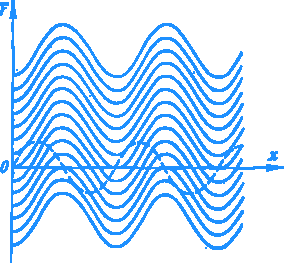
\includegraphics[width=0.6\textwidth]{figures/fig-44.pdf}
\caption{Graphs of the anti-derivatives of the function $f (x) = \sin x$.}
\label{fig-44}
\end{figure}

The figure clearly shows that all the antiderivatives belong to one family (in other words, correspond to the same initial function $f$). This may not always be as clear if the function is represented in an analytical form. Take, for
example, functions $F_{1} =-\cos x$ and $F_{2} =3- 2	\cos^{2} \dfrac{x}{2}$. It would be difficult to say at the first glance that these two
functions are the antiderivatives of \emph{one and the same function} (namely, $f = \sin x$). However, since $2 \cos^{2} \dfrac{x}{2} = 1 + cos x$, we find
\begin{equation*}%
F_{2}(x) = 3- 1 - \cos x =- \cos x + 2
\end{equation*}
\rdr I guess it would be possible to find directly that $F_{1}' (x) = F_{2}' (x)$, wouldn't it?

\athr Of course, it would:
\begin{align*}%
\ddx F_{2} (x) & = -2 \ddx \cos^{2} \dfrac{x}{2}  = 4 \cos \dfrac{x}{2} \sin \frac{x}{2} \cdot \frac{1}{2} = \sin x\\
& \\
\ddx F_{1} (x) & = \ddx (- \cos x) = \sin x
\end{align*}
But the easiest way is to notice that $F_{2} - F_{1} = C$. 

We could find numerous such examples. For instance, it is not difficult to check that the following pairs of functions belong to the same family of antiderivatives (each pair to its own family): 
\begin{enumerate}[label=(\alph*)]
\item $F_{1} = x^{2} - 2x + 3, \,\, F_{2} = (x- 1)^{2}$
\item $F_{1} = \arcsin x, \,\, F_{2} = 1 - \arccos x $
\item $F_{1} = \tan x \, \sin x + \cos x, \,\, F_{2} = (2 \cos x + 1) \dfrac{1}{ \cos x}$
\end{enumerate}
Thus, in case (a) we find $F_{2} -	F_{1} = -2$; both functions are the antiderivatives of the function $f = 2x - 2$.

Please, check cases (b) and (c) yourself. 

\rdr In case (b)  $F_{2} - F_{1} = (1 - \arccos x +
+ \arcsin x) = 1 - \dfrac{\pi}{2}$ both functions are the antiderivatives of the function $f = \dfrac{1}{1 - x^{2}}$

Case (c) is more intricate. Some preliminary manipulations are necessary:
\begin{align*}%
F_{1} (x) & = \tan x \sin x + \cos x = \dfrac{\sin^{2} x + \cos^{2} x}{\cos x} = \dfrac{1}{\cos x}\\
& \\
F_{2} (x) & = \frac{2 \cos x + 1 }{\cos x} = 2 + \dfrac{1}{\cos x}
\end{align*}
Therefore, $F_{2} - F_{1}=2$. Both functions ($F_{1}$ and $F_{2}$) are the antiderivatives of $f = \dfrac{\sin x}{\cos^{2} x}$

\athr Correct. Now, taking into account the results obtained in the previous dialogue, we can compile a table (see  \hyperref[deriv-list]{Table 2}) which gives various functions $f (x)$ in the first column the corresponding derivatives $f' (x)$ in the second column, and the antiderivatives $F (x) + C$, corresponding to the functions $f (x)$, in the third column. I want to stress once more: the transformation $f (x) \to f' (x)$ is the operation of differentiation of the function $f(x)$, and the transformation $f (x) \to [F (x) + C]$ is the operation of integration of the function $f (x)$.

\newpage 
%\vspace*{2cm}

\begin{center}
\textcolor{DodgerBlue}{\textbf{A List of Derivatives and Antiderivatives for Selected Functions}}\\[30pt]
%{\smaller
%\boxed{
\begin{tcolorbox}[colback=white,colframe=DodgerBlue]
\centering
\begin{tabular}{l>{\color{IndianRed}}r>{\color{IndianRed}}r>{\color{IndianRed}}r}
%\toprule
 & Function & Derivative & Antiderivative \\
  & $f(x)$ & $f'(x)$ &  F(x) \\
 \arrayrulecolor{DodgerBlue} \toprule
\circled{\rownumber} & $a$ & 0 & $ax + C$\\
    \arrayrulecolor{DodgerBlue}\midrule
\circled{\rownumber} & $x^{n}$ & $n x^{n-1}$ & $\dfrac{1}{n+1} x^{n+1} + C$\\
\midrule
\circled{\rownumber} & $e^{x}$ & $e^{x}$ & $e^{x} + C$\\
\midrule
\circled{\rownumber} & $\dfrac{1}{x}$ & $-\dfrac{1}{x^{2}}$ & $\ln x + C$\\
\midrule
\circled{\rownumber} & $\sqrt{x}$ &  $\dfrac{1}{2\sqrt{x}}$ & $\dfrac{2}{3} x  \sqrt{x} + C$\\
\midrule
\circled{\rownumber} & $\sin x$ & $\cos x$ & $- \cos x + C$\\
\midrule
\circled{\rownumber} & $\cos x$ & $-\sin x$ & $\sin x + C$\\
\midrule
\circled{\rownumber} & $\dfrac{1}{\cos^{2}} x$ & $2 \dfrac{\sin x}{\cos^{3} x}$ & $- \cot x + C$\\
\midrule
\circled{\rownumber} & $\dfrac{1}{\sin^{2} x}$ & $-2 \dfrac{\cos x}{\sin^{3} x}$ & $\tan x + C$\\
\midrule
\circled{\rownumber} & $\dfrac{1}{1 + x^{2}}$ & $-\dfrac{2 x}{ (1+x^{2})^{2}}$ & $\arctan x + C$\\
\label{deriv-list}
\end{tabular}
%}
\end{tcolorbox}
\end{center}

\newpage

\rdr Examples \circled{8}, \circled{9}, and \circled{10} in \hyperref[deriv-list]{Table 2} give an impression that the transformation $f (x) \to f' (x)$ is more complicated than the transformation $f (x) \to [F (x) + C]$.

\athr This impression stems from a special selection of the functions $f (x)$. Thus, it is easier to differentiate the function $\tan x$ than the function $\dfrac{1}{\cos^{2} x}$. Indeed, in the latter case we have to use the rules for differentiation of a ratio of two functions or of a composite function. 

In general, it should be noted that the operation of integration is substantially more complicated than that of differentiation. The differentiation of elementary functions invariably gives elementary functions. By employing the rules for differentiation discussed in the previous dialogue, you will be able (and with no difficulties, as a rule) to differentiate practically any elementary function. But integration is quite a different proposition. The rules for the integration of elementary functions comprise numerous techniques, and we would need several special dialogues to scan them. But the main point is that not every elementary function has an elementary function for its antiderivative. As one example, I shall mention the antiderivatives of such elementary
functions as $\dfrac{1}{\log x}$ or $\dfrac{1}{ \sqrt{1 + x^{2}}} $.
 As a rule, in such cases one is forced to resort to the methods of the so-called \emph{numerical integration}.

\rdr I was very attentive and want to pose two questions. First: What is meant by the term \emph{elementary function}?

\athr In \hyperref[derivative]{Dialogue Nine} I gave examples of the so-called \emph{fundamental elementary functions} ($x^{n}, \, x^{-n}, \, x^{1/n}, \, \sin x, \, \cos x,$ $\,	\tan x, \,	\cot x,	\, \arcsin x,$ $\,	\arccos x,	\, \arctan x, \,	\arccot x, \, a^{x}, \, \log_{a} x$]. An \emph{elementary function} is any function which can be formed of \emph{fundamental elementary functions} by a \emph{finite} number of the operations of addition, subtraction, multiplication, division, involution, evolution, and taking a modulus, as well as by using the rules for obtaining inverse and composite functions. All the functions used in the previous dialogues are elementary (with an exception of the Dirichlet function mentioned in \hyperref[{more-on-function}]{Dialogue Five}), and many of them are fundamental elementary functions.

\rdr My second question concerns the \emph{rules for integration} you refer to. Could you give at least some examples?

\athr I shall quote three simplest rules.
\begin{mytheo}{Three Simple Rules for Integration}
\begin{enumerate}[label=\protect\circled{\arabic*}]
\item If $F$ is an antiderivative for $f$. and $G$ is an anti-derivative for $g$, an antiderivative for the sum of the functions $f + g$ is a function $F + G$.
\item If $F$ is an antiderivative for $f$ an antiderivative for a function $af$, where $a$ is a constant, is a function $aF$.
\item If $F (x)$ is an antiderivative for $f (x)$, and $a$ and $b$ are constants, an antiderivative for a function $f (ax + b)$ is a function $\dfrac{1}{a} F (ax + b)$.
\end{enumerate}
\end{mytheo}
All the three rules are proved readily by using the rules for differentiation (in the third rule one has to apply the rule for the differentiation of composite functions). Indeed,
\begin{enumerate}[label=\protect\circled{\arabic*}]
\item $\ddx (F+G) = \ddx F + \ddx G= f + g$ 
\item $\ddx (aF)= a \ddx F= af$
\item $\begin{aligned}[t]%
\ddx \left( \frac{1}{a} F (ax + b)  \right)  & = \frac{1}{a} \ddx F(ax +b) =  \frac{1}{a} \dfrac{d}{dy} F(y) \ddx (ax +b) \\
& =  \frac{1}{a} f(y)\, a = f(y) = f(ax +b) 
\\ & \text{here:} \,\, y = ax +b
\end{aligned}$
\end{enumerate}
Of course, the three rules cited above do not exhaust a rich collection of integration rules available in calculus. 

But here these three rules will be sufficient since our goal is quite modest: to give the fundamental idea of an anti-derivative.

\rdr Our discussion of a derivative covered its geometrical interpretation as well. Is there a geometrical  interpretation of an antiderivative?

\athr Yes, there is. Let us find it (besides, we shall need it later).

Consider a function $f (x)$. For the sake of simplicity, assume that this function is \emph{monotonic} (and even \emph{increasing}). Later we shall drop the monotonicity of a function. The most important is that the function be \emph{continuous} over the chosen interval (i.e. over the interval on which it is defined). \fig{fig-45} shows a shaded area (the so-called \emph{curvilinear trapezoid}) bounded by the graph of the function $f (x)$, the interval $[a, x]$ of the $x$-axis, and two perpendiculars	erected from points $a$ and $x$ on the $x$-axis. Let point $a$ be fixed; as for point $x$ (the right-hand end of the interval $[a, \, x]$), it is not fixed and can assume values from a upward (within the domain of definition of the function). Obviously, the \emph{area} of the curvilinear trapezoid shaded in the figure is a \emph{function} of $x$. We shall denote it by $S (x)$,

\begin{figure}[!ht]%[13]{r}{0.5\textwidth}
\centering
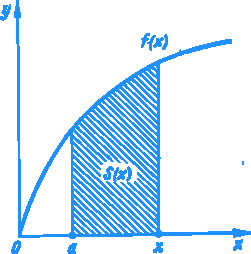
\includegraphics[width=0.5\textwidth]{figures/fig-45.pdf}
\caption{Examining the geometrical interpretation of the antiderivative.}
\label{fig-45}
\end{figure}

Now turn to \fig{fig-46}. Let us give an increment $\Delta x$ to the independent variable $x$. The interval $[a, \, x + \Delta x]$ corresponds to the area $S (x + \Delta x)$. Denote $\Delta S(x) = S (x + \Delta x)- S (x)$. The increment $\Delta S(x)$ is, obviously, the area of the shaded curvilinear trapezoid. The figure shows that
\begin{equation*}%
\text{area} \,\, ADEF < \Delta S (x) < \text{area} \,\, ABCF 
\end{equation*}

\begin{figure}[!ht]%[13]{r}{0.5\textwidth}
\centering
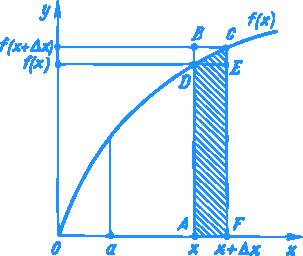
\includegraphics[width=0.6\textwidth]{figures/fig-46.pdf}
\caption{Examining the geometrical interpretation of the antiderivative.}
\label{fig-46}
\end{figure}

But the area $ADEF$ is equal to $f (x) \Delta x$, and the area $ABCF$
is equal to $f (x +  \Delta x) \Delta x$. Therefore,
\begin{equation*}%
\text{area} \,\, ADEF < \Delta S (x) < \text{area} \,\, ABCF 
\end{equation*}
or
\begin{equation*}%
f (x) \Delta x < \dfrac{\Delta S (x)}{ \Delta x}  < f (x + \Delta x)
\end{equation*}
or
\begin{equation*}%
0 < \left(  \dfrac{\Delta S (x)}{ \Delta x}  - f (x) \right) < [f (x) + \Delta x)-	f (x)] = \Delta f(x) 
\end{equation*}

Now we find the limiting values of these inequalities for $\Delta x$ tending to zero. By virtue of the continuity of the function $f (x)$ we conclude that $\lmts{\Delta x}{0} \Delta f (x) = 0$. Consequently,
\begin{equation*}%
\lmts{\Delta x}{0} \left(  \dfrac{\Delta S (x)}{ \Delta x}  - f (x) \right) = 0
\end{equation*}
As the function $f (x)$ is independent of $\Delta x$, the last relation yields
\begin{equation}%
\lmts{\Delta x}{0}  \dfrac{\Delta S (x)}{ \Delta x}  = f (x)
\label{antideriv-geom1}
%eq 2 of 11
\end{equation}
By the definition of derivative,
\begin{equation*}%
\lmts{\Delta x}{0}  \dfrac{\Delta S (x)}{ \Delta x}  = S' (x)
\end{equation*}
Consequently, relation \eqref{antideriv-geom1} signifies that
\begin{equation}%
 f (x)  = S' (x)
\label{antideriv-geom2}
%eq 3 of 11
\end{equation}

Thus, in terms of geometry, \emph{the antiderivative of the function $f$, taken at point $x$, is the area of curvilinear trapezoid bounded by the graph of the function $f (x)$ over the interval $[a, x]$ of the $x$-axis}.

\rdr Presumably, it is one of the possible anti-derivatives, isn't it?

\athr Definitely.

\rdr But it is evident that the area $S (x)$ also depends on the choice of point $a$.

\athr Absolutely correct. By choosing different points $a$, we shall have different areas of curvilinear trapezoids and, correspondingly, different antiderivatives. But all of them will be the antiderivatives of the function $f$ taken at point $x$. It is only important that in all cases $a < x$.

\rdr Then why is it that point $a$ vanishes from the final results?

\athr Your bewilderment is understandable. Let us reformulate the results obtained above. Let $F (x)$ be an antiderivative of a function $f (x)$ taken at point $x$. According to \eqref{antideriv-geom2}, we can write
\begin{equation*}%
S(x) = F(x) + C
\end{equation*}
(here we have used the following theorem: if two functions have equal derivatives, the functions will differ by a constant term). The constant $C$ is found readily since $S (a) = 0$. Therefore,
\begin{equation*}%
S (a) = F (a) + C = 0
\end{equation*}
Hence, $C = -F (a)$. This gives
\begin{equation}%
S(x)=F(x)- F(a)
\label{antideriv-geom3}
%eq 4 of 11
\end{equation}

\begin{mytheo}{Conclusion}
If $F (x)$ is an antiderivative of a function $f (x)$, then the area $S (x)$ of a curvilinear trapezoid bounded by the graph of the junction $f (x)$ over the interval $[a, x]$ is given by the difference $F (x)- F (a)$.
\end{mytheo}
You see now that point $a$ is introduced explicitly. 

\rdr Now everything is clear, 

\athr Relation \eqref{antideriv-geom2} (and from it, \eqref{antideriv-geom3}) can be obtained for every continuous function; the \emph{monotonicity} of a function is \emph{not} a necessary condition. Consider a function $f (x)$ whose graph is plotted in \fig{fig-47}. We choose a point $x$ and wish to prove that for any $\varepsilon > 0$ there is $\delta > 0 $ such that
\begin{equation}%
\left|  \dfrac{\Delta S (x)}{ \Delta x}   - f(x) \right| < \varepsilon
\label{antideriv-geom4}
%eq 5 of 11
\end{equation}

for all $\Delta x$ satisfying the condition $| \Delta x |<  \delta$. 

\begin{figure}[!ht]%[13]{r}{0.5\textwidth}
\centering
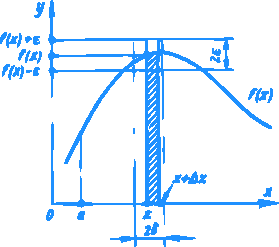
\includegraphics[width=0.6\textwidth]{figures/fig-47.pdf}
\caption{Examining the geometrical interpretation of the antiderivative.}
\label{fig-47}
\end{figure}

\rdr Shall we consider point $x$ as fixed? 

\athr Yes. Increments $\Delta x$ and, correspondingly,
$\Delta S (x)$, are always considered for a definite point $x$.
So we take an arbitrary number $\varepsilon > 0$ (shown in the figure).  As f (x) is a continuous function, there is a number $\delta > 0$ such that 
\begin{equation}%
|f(x) + \Delta x - f(x)| < \varepsilon
\label{antideriv-geom5}
%eq 6 of 11
\end{equation}
for all $\Delta x$ satisfying the condition $| \Delta x | < 0$. This number $\delta$ is the one we were to find.

Indeed, let us choose, for definiteness, that $\Delta x > 0$ but specify that $\Delta x < \delta$. The area of the curvilinear trapezoid shaded in \fig{fig-47} will be denoted by $\Delta S (x)$ (this trapezoid is bounded by the graph of the function $f (x)$ over the interval $[x, \, x + \Delta x]$. Inequality \eqref{antideriv-geom5} yields (see the figure):
\begin{equation*}%
[f(x)  -   \varepsilon] \Delta x < \Delta S (x) < [f(x) - \varepsilon] \Delta x
\end{equation*}
or
\begin{equation*}%
[f(x)  -   \varepsilon]  < \dfrac{\Delta S (x)}{\Delta x} < [f(x) - \varepsilon]
\end{equation*}
or, 
\begin{equation*}%
 -  \varepsilon < \left( \dfrac{\Delta S (x)}{\Delta x} - f(x) \right)  < \varepsilon 
\end{equation*}
or, finally.
\begin{equation*}%
\left| \dfrac{\Delta S (x)}{\Delta x} - f(x) \right|  < \varepsilon
\end{equation*}
which is what we wanted to prove.

You see that a function $f$ needn't be monotonic: relation \eqref{antideriv-geom2} (and with it, \eqref{antideriv-geom3} is easily generalized to the case of an arbitrary continuous function $f$.

Now let us turn again to \fig{fig-44} that gives a family of graphs of the antiderivative $F (x) = - \cos x + C$ for the function $f (x) = \sin x$. Indicate which of these graphs (which antiderivative) stands for $S (x)$ in each of the following three cases: 
\begin{enumerate*}[label=(\alph*)]
\item $a = 0$, 
\item $a = \dfrac{\pi}{2}$, and 
\item $a = \pi$. 
\end{enumerate*}

\rdr The question is clear. I denote the sought functions	by	$S_{1} (x), \, S_{2}	(x)$, and $ S_{3} (x)$, respectively.	These functions are plotted in \fig{fig-48}.

Obviously, we can write
\begin{align*}%
S_{1}(x) & = F(x) - F(0) \\
S_{2}(x) & = F(x) - F(\dfrac{\pi}{2})\\
S_{3}(x) &= F(x) - F(\pi)
\end{align*}

\athr  Correct. It is important to underline that in each of the above three equalities the function $F (x)$ is a function chosen arbitrarily from the family of antiderivatives of $f$, shown in \fig{fig-44}.

\begin{figure}[!ht]%[13]{r}{0.5\textwidth}
\centering
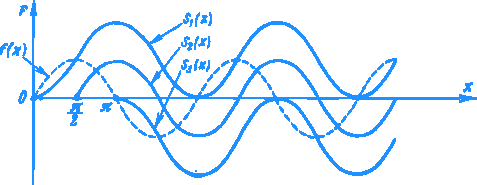
\includegraphics[width=\textwidth]{figures/fig-48.pdf}
\caption{Particular graphs of the antiderivative for specific value of $a$.}
\label{fig-48}
\end{figure}

\rdr It looks as if whatever the selected antiderivative of the function $f$ is, the difference between its values at two points depends only on the choice of these points but not on the choice of a specific antiderivative.

\athr You have pointed out a property of principal significance. It is so important that deserves a special dialogue.
% !TEX root = calculus.tex


\chapter{INTEGRAL}
\label{integral}

\athr We know already that the difference between the values of an antiderivative at two arbitrary points depends only on the choice of these points (and, evidently, on the type of the initial function $f (x))$. As these two points we choose points $a$ and $b$, that is, consider an increment of an antiderivative, $F (b) - F (a)$, This increment plays a very important role among the tools of calculus; it is called the \emph{integral}.
\begin{mytheo}{Definition}
The increment of an anti-derivative $F$ of a function $f$, i,e. $F(b)- F(a)$, is said to be the integral of $f$ from $a$ to $b$.
\end{mytheo}
The notation of the integral is:
\begin{equation*}%
\int_{a}^{b} f(x) \, dx
\end{equation*}
(it reads: ``integral of $f$ of $x$, $dx$, from $a$ to $b$''). The numbers $a$ and $b$ are the \emph{lower} and \emph{upper limits of integration}. The function $f$ is said to be \emph{integrand}, and $x$ the \emph{integration variable}.

Consequently, if $F$ is one of the antiderivatives of the function $f$, then the definition of an integral states that 
\begin{equation}%
\boxed{\int_{a}^{b} f(x) \, dx = F(b)- F(a)}
\label{newton-lebnitz-formula}
% eq 1 of 12
\end{equation}

Formula \eqref{newton-lebnitz-formula} is known in the literature on mathematics as the \emph{Newton-Leibnitz formula}. Remember that $F$ here is an arbitrary antiderivative of the function $f$.
\begin{figure}[!ht]%[13]{r}{0.5\textwidth}
\centering
\includegraphics[width=.9\textwidth]{figures/fig-49.pdf}
\caption{Examining the geometrical interpretation of the integral as area.}
\label{fig-49}
\end{figure}

\rdr As far as I understand, the integral of the function $f$ from $a$ to $b$ is precisely the area of the curvilinear trapezoid bounded by the graph of the function $f (x)$ over the interval $[a, b]$. Is that right?

\athr Absolutely. The expression
\begin{equation*}%
\int_{a}^{b} f(x) \, dx
\end{equation*}
is nothing less than the area of this geometrical figure. \fig{fig-49} shows three cases plotting different integrands:
\begin{enumerate*}[label=(\alph*)]
\item $f(x) = 2x$, 
\item $f(x) = x^{2}$,
\item $f(x) = \sqrt{x}$. 
\end{enumerate*}

The limits of integration are chosen identical in all the three cases: $a = 1, \, b = 2$. The corresponding areas of the curvilinear trapezoids are shaded in the figure:
\begin{align*}%
S_{1} & = \int_{1}^{2} 2 x \, dx \\
S_{2} & = \int_{1}^{2} x^{2} \, dx \\
S_{3} & = \int_{1}^{2} \sqrt{x} \, dx
\end{align*}
The numbers $S_{1}, \, S_{2}$,	and $S_{3}$ are different because the integrands $f (x)$ are different.

We thus find that the expression
\begin{equation*}%
\int_{a}^{b} f(x) \, dx
\end{equation*}
works as a \emph{functional} (recall Dialogue Four). You ``input'' in it a function $f$, and it ``outputs'' a number $S$.

By the way, you can easily find how this functional works. To achieve this, use formula \eqref{newton-lebnitz-formula} and take into account that the antiderivative of the function $f (x) = 2x$ is $F (x) = x^{2} + C$, that of $f(x) = x^{2}$ is $F(x) = \dfrac{1}{3} x^{3}+C$, and that of $f(x) =\sqrt{x}$ is  $F(x) = \dfrac{2}{3} x \sqrt{x} +C$.

The standard notation is: $F (b) - F (a) = F (x) |_{a}^{b}$. Therefore,
\begin{align*}%
\int_{1}^{2} 2 x \, dx & = x^{2} |_{1}^{2} = 4 - 1 = 3 \\
\int_{1}^{2} x^{2} \, dx & = \dfrac{1}{3} x^{3}|_{1}^{2} =  \dfrac{1}{3} (8 -1) =  \dfrac{7}{3} \\
 \int_{1}^{2} \sqrt{x} \, dx & = \dfrac{2}{3} x \sqrt{x} |_{1}^{2} =  \dfrac{2}{3} (2 \sqrt{2} -1)
\end{align*}

With the function $2x$ at the ``input'' of the functional $\int_{1}^{2} f(x) \, dx $, we obtain at the ``output'' the number 3; with $x^{2}$ at the ``input'', we obtain at the ``output'' the number $\dfrac{7}{3}$; and with $\sqrt{x}$ at the ``input'', we obtain at the ``output'' the number  $\dfrac{2}{3} (2 \sqrt{2} -1)$.

\rdr I see that we can rather easily find the areas of various curvilinear trapezoids!

\athr More than only curvilinear trapezoids. For instance, try to find the area of the figure shaded in \fig{fig-50}. 

\begin{figure}[!ht]%[13]{r}{0.5\textwidth}
\centering
\includegraphics[width=.45\textwidth]{figures/fig-50.pdf} 
\caption{Curvilinear trapezoids as integral of a function.}
\label{fig-50}
\end{figure}

\rdr This area is the difference between the areas
of two curvilinear trapezoids: 
\begin{equation*}%
S = \int_{0}^{1} \sqrt{x} \, dx -  \int_{0}^{1} x^{2} \, dx
\end{equation*}
Therefore,
\begin{equation*}%
S = \dfrac{2}{3} x \sqrt{x} |_{0}^{1} -  \dfrac{1}{3} x^{3} |_{0}^{1} = \dfrac{2}{3} 	 - \dfrac{1}{3} = \dfrac{1}{3}
\end{equation*}

\athr Correct. Consider another example. Find the area of the shaded figure in	\fig{fig-51}.

\begin{figure}[!ht]%[13]{r}{0.5\textwidth}
\centering
\includegraphics[width=.45\textwidth]{figures/fig-51.pdf}
\caption{Curvilinear trapezoid as the integral of a function.}
\label{fig-51}
\end{figure}

\rdr The graphs of the functions $\sin x$ and $\cos x$ intersect at the point $x = \dfrac{\pi}{4}$. Consequently, one has to use the antiderivative of the function $\sin x$ over the interval $\left[ 0, \, \dfrac{\pi}{4} \right]$ and that of the function $\cos x$ over the interval $\left[  \dfrac{\pi}{4}, \, \dfrac{\pi}{2} \right]$. Hence,
\begin{align*}%
S & = \int_{0}^{\frac{\pi}{4}} \sin x \, dx + \int_{\frac{\pi}{4}}^{\frac{\pi}{2}} \cos x \, dx  = - \cos x |_{0}^{\frac{\pi}{4}}  + \sin x |_{\frac{\pi}{4}}^{\frac{\pi}{2}} \\
& = - \left(\cos \frac{\pi}{4} - \cos 0 \right) + \left(\sin \frac{\pi}{2} - \sin \frac{\pi}{4}  \right) \\
& = - \left( \frac{\sqrt{2}}{2} - 1 \right) + \left(1 - \frac{\sqrt{2}}{2}  \right) \\
& = 2 - \sqrt{2}
\end{align*}

\athr Perfectly right. Now we shall discuss one ``fine point'', returning to formula \eqref{newton-lebnitz-formula} and rewriting it in the form
\begin{equation}%
\boxed{\int_{a}^{x} f(t) \, dt = F(x)- F(a)}
\label{newton-lebnitz-formula2}
% eq 2 of 12
\end{equation}
What has been changed by this rewriting? 

\rdr First, we have replaced the \emph{constant} upper limit of integration (the number $b$) by the \emph{variable} limit of integration (the variable $x$). Second, we have substituted the integration variable $t$ for the integration variable $x$.

\athr Only the first of these changes is significant. The second (the substitution of the integration variable) is of no consequence. It is easy to see that the formulas
\begin{equation*}%
\int_{a}^{b} f(x) \, dx \,\, \int_{a}^{b} f(t) \, dt \,\, \int_{a}^{b} f(y) \, dy \,\, \int_{a}^{b} f(z) \, dz
\end{equation*}
are \emph{equivalent} since all the four give $F (b) - F (a)$. So it does not matter what \emph{symbol} is used for the integration variable in each particular case.

\rdr Why, then, did you have to substitute the variable $t$ for the integration variable $x$ in \eqref{newton-lebnitz-formula2}?

\athr Only not to confuse the integration variable with the variable upper limit. These are different variables and, of course, must be denoted by different symbols.
The expression
\begin{equation*}%
\int_{a}^{x} f(t) \,\, dt
\end{equation*}
is called the \emph{integral with a variable upper limit}. It is important that in contrast to the expression
\begin{equation*}%
\int_{a}^{b} f(t) \,\, dt
\end{equation*}
this expression yields not a number but a function. According to \eqref{newton-lebnitz-formula2}, this function is $F (x) - F (a)$.

\rdr But if the $\displaystyle\int_{a}^{b} \Box dt$ ``black box'' is a \emph{functional}, then the $\displaystyle\int_{a}^{x} \Box dt$ ``black box'' is an operator? (I have used
here our symbolic notation of ``windows'' into which the function $f$ must be input).

\athr Correct. This is immediately clear in the following unusual table.

\begin{center}
\textcolor{DodgerBlue}{\textbf{An Unusual Table}}\\[20pt]
%{\smaller
\boxed{
\begin{tabular}{>{\color{IndianRed}}c>{\color{IndianRed}}c>{\color{IndianRed}}c}
%\toprule
   $f(x)$ & $\int_{1}^{2} f(t) \,\, dt$ &  $\int_{1}^{x} f(t) \,\, dt$ \\
    \arrayrulecolor{DodgerBlue} \toprule
$2x$ & 3 & $x^{2} -1 $\\
\midrule
$3x^{2}$ & 7 & $x^{3} -1 $\\
\midrule
$4x^{3}$ & 15 & $x^{4} -1 $\\
\midrule
$5x^{4}$ & 31 & $x^{5} -1 $\\
\midrule
$6x^{5}$ & 63 & $x^{6} -1 $
\end{tabular}
}
\end{center}
The second and third columns of this table show \emph{what} the
``output'' of the two ``black boxes'',  $\displaystyle\int_{1}^{2} f(t) \,\, dt$ and  $\displaystyle\int_{1}^{x} f(t) \,\, dt$, is when the ``input'' is a function $f$ of the first column.

The integral $\displaystyle\int_{a}^{x} (\ldots) \,\, dt$ is thus indeed an operator. Note that its effect on a function is \emph{opposite} to that of the operator $\ddx$ (we discussed this operator in Dialogue Nine).

Indeed, take a function $f$ and first apply to it the operator $\displaystyle\int_{a}^{x} (\ldots) \,\, dt$ and then the operator $\ddx: \,\, \ddx \left( \displaystyle\int_{a}^{x} (\ldots) \,\, dt \right) $.
This gives
\begin{equation*}%
\ddx \left( \int_{a}^{x} (\ldots) \,\, dt \right) = \ddx [F(x) - F(a)]  = \ddx F(x) = f(x)	
\end{equation*}
i.e. we obtain the initial function $f$. 

\rdr We could apply these operators to the function in the \emph{reverse} order, couldn't we?

\athr Yes, we could. This means that the expression
\begin{equation*}%
 \int_{a}^{x} \left( \dfrac{d}{dt} f(t) \right) \,\, dt
\end{equation*}
also gives the initial function $f$. At least, to within a constant term.

\rdr Can it be verified?

\athr Yes, and very easily. What function is the antiderivative for $f' (x)$?

\rdr Obviously, the function $f (x) + c$. 

\athr Therefore,
\begin{equation*}%
 \int_{a}^{x} \left( \dfrac{d}{dt} f(t) \right) \,\, dt =  \int_{a}^{x} f'(t) \,\, dt = f(x) - f(a)
\end{equation*}

\rdr Will it be correct to say that while the operator $\ddx$ performs the \emph{operation of differentiation}, the operator $\displaystyle\int_{a}^{x} (\ldots) \,\, dt$ performs the \emph{operation of integration}?

\athr Precisely. It might seem that the topic is exhausted, but the discussion would be incomplete without a clarification of one essential ``subtlety''. Throughout this dialogue we operated with something we called ``the area of a curvilinear trapezoid'' and found that this is the meaning of the integral. But what is the ``area of a curvilinear trapezoid?''

\rdr But surely this is self-evident. One glance at the figures is enough.

\athr Look, for instance, at \fig{fig-45}. It shows a shaded geometrical figure called a curvilinear trapezoid. But it says nothing about the \emph{area} of the trapezoid.

\rdr The area is a standard concept in geometry.

\athr No objections. But do not forget that in geometry you normally apply this concept to a well-defined set of figures: triangles, trapezoids, etc. And you remember that difficulties arise when you try to determine the \emph{area of a circle}. By definition, the area of a circle is the limit of the sequence of the areas of regular polygons inscribed in, or circumscribed around, the circle, for an infinitely increasing number of the sides of the polygon.

\rdr Presumably, the area of a curvilinear trapezoid can also be defined as the \emph{limit of a specific sequence of areas}? 

\athr Yes, this is the normal approach. Consider a curvilinear trapezoid bounded by the graph of a function $f (x)$ over the interval $[a, b]$ (\fig{fig-52}). Let us subdivide the interval $[a, b]$ into n subintervals of identical length $\Delta x = \dfrac{b-a}{n}$ (in \fig{fig-52} $n = 10$). The end points of these n
subintervals are denoted from left to right: 
\begin{equation*}%
x_{0} = a, \, x_{1}, \, x_{2}, \,x_{3}, \, \ldots x_{n} = b
\end{equation*}
On each $\Delta x$-long interval, used as a base, we construct a \emph{rectangle} of altitude $f (x_{k-1})$, where $k$ is the subscript of the right-hand end of this subinterval (this choice is arbitrary; the left-hand end would do equally well). The area of this rectangle is
\begin{equation*}%
f (x_{k-1}) \, \Delta x
\end{equation*}
Consider now a sum of the areas of all such rectangles (this
total area is shaded in \fig{fig-52}): 
\begin{align*}%
S_{n} (a, b) & = f(x_{0}) \Delta x +  f (x_{1}) \Delta x + \ldots + f (x_{n-1}) \Delta x \\
& = [f(x_{0})  +  f (x_{1})  + \ldots + f (x_{n-1})] \,\, \dfrac{b-a}{ n}
\end{align*}
As the function $f (x)$ is continuous, the ensemble of all these rectangles for sufficiently large $n$ (sufficiently small $\Delta x$) will be very close to the curvilinear trapezoid in question, and, at any rate, the closer the larger $n$ is (the smaller $\Delta x$). It is, therefore, logical to assume the following definition:

\begin{figure}[!ht]%[13]{r}{0.5\textwidth}
\centering
\includegraphics[width=.6\textwidth]{figures/fig-52.pdf} 
\caption{Curvilinear trapezoids as integral of a function.}
\label{fig-52}
\end{figure}

\begin{mytheo}{Definition:}
The sequence of sums $(S_{n} (a, b))$ with $n$ tending to infinity has the limit said to be the area of the given curvilinear trapezoid $S (a, b)$:
\begin{equation}%
S(a,b)= \lmts{n}{\infty} S_{n} (a, \, b)
\label{area-of-trapezoid}
% eq 3 of 12
\end{equation}
\end{mytheo}

\rdr The area $S (a, b)$ of a curvilinear trapezoid was shown earlier to be the integral $\displaystyle\int_{a}^{b} f(x) \,\, dx$; consequently, definition \eqref{area-of-trapezoid} is a new definition of the integral:
\begin{equation}%
\boxed{\int_{a}^{b} f(x) \, dx = \lmts{n}{\infty} S_{n} (a, \, b)}
\label{int-def-2}
% eq 4 of 12
\end{equation}
Do you agree? 

\athr Yes, certainly. And note that definition \eqref{int-def-2}
is \emph{independent}, that is, it is not based on the concept of the antiderivative.

Historically, by the way, the integral appeared as \eqref{int-def-2}, the fact that explains the origin of the standard notation. Indeed, if definition \eqref{int-def-2} is rewritten in a slightly different form
\begin{equation}%
\int_{a}^{b} f(x) \, dx = \lmts{n}{\infty} \left( \sum_{k=1}^{n} f(x_{k-1}) \Delta x \right)
\label{int-def-3}
% eq 5 of 12
\end{equation}
you may notice a certain similarity in the form of the left- and right-hand sides of this equality. The very symbol $\int$( the integral sign) originated from the letter $S$ which was often used to denote sums. The product $f(x_{k-1}) dx$ evolved to $f (x) dx$. In the 17th century mathematicians did not use the concept of the limit. They treated integrals as ``sums of an infinitely large number of infinitely small addends'', with $f (x) dx$ being these infinitesimal addends. In this sense, the area of a curvilinear trapezoid $S$ was defined as the ``sum of an infinitely large number of infinitely small areas $f (x) dx$.''

You realize, I hope, that such concepts were obviously lacking mathematical rigorousness.

\rdr This illustrates what you termed on many occasions ``subjective impressions''.

\athr It must be clear to you by now that a strict mathematical interpretation of the concept of the \emph{integral} is possible only if the \emph{limit transition} is used. I have already emphasized that the limit transition is the foundation of calculus. If the concept of the limit is avoided (``limit of sequence'' or ``limit of function''), neither the derivative nor integral can he treated rigorously.

\rdr But the integral can be defined without resorting to  \eqref{int-def-2}. It is quite sufficient to use the Newton-Leibnitz formula \eqref{newton-lebnitz-formula}. And this formula does not involve any limit transitions.

\athr But this formula involves the antiderivative. And the antiderivative involves, in the long run, the concept of the derivative, that is, the unavoidable limit transition.

By the way, your last remark makes me touch the aspects of introducing the integral in the literature. Two methodically distinct approaches are possible. 

The \emph{first approach} (the one used in those dialogues) assumes
that the operation of integration is directly introduced as an operation inverse to differentiation. The Newton-Leibnitz formula \eqref{newton-lebnitz-formula} then serves, in fact, as the definition of the integral: it is defined as an \emph{increment of the anti-derivative}.

The \emph{second approach} assumes that the operation of integration is introduced as an \emph{independent} operation, the integral being defined as the \emph{limit} of a sequence formed of the appropriate sums (see formula  \eqref{int-def-2}). This approach corresponds to the historical progress in mathematics; indeed, originally integral calculus was evolving independently of differential calculus. The profound relationship between the two branches of mathematics had been discovered only by the end of the 17th century when the main problems of the two were understood as \emph{mutually inverse}. The Newton-Leibnitz formula \eqref{newton-lebnitz-formula} was precisely a reflection of this relationship: it was demonstrated that the integral is none other than an increment of the antiderivative.
% !TEX root = calculus.tex


\chapter{DIFFERENTIAL EQUATIONS}
\label{diff-eqns}

\athr You are, certainly, familiar with various types of equations: algebraic, logarithmic, exponential, trigonometric. They have a common feature: by solving these equations one arrives at \emph{numbers} (these are the so-called ``roots'' of equations). Now we are going to deal with a very different type of equations, namely, \emph{equations whose solutions are functions}. Among the equations subsumed into this class are the so-called \emph{differential equations}.

Consider a function $f (x)$. We denote its first derivative (the first-order derivative) by $f' (x)$, its second derivative by $f''(x)$, its third derivative by $f''' (x)$, and so on.

\begin{mytheo}{Definition:}
A differential equation is an equality relating $x, \, f (x), \, f' (x), \, f'' (x)$, etc. A solution of a differential equation is a junction $f (x)$.
\end{mytheo}
\rdr So far you have never mentioned the concepts of second derivative or third derivative.

\athr True, and this is what we are going to do right now.

\rdr It is readily apparent that since a derivative $f (x)$ is a \emph{function}, it can be differentiated, thus yielding a \emph{derivative of the derivative}; I guess, this must be the second derivative of the original function $f (x)$.

\athr By differentiating the function $f (x)$ $n$ times o(of course, if this can be done with the given function), we obtain a derivative of the $n$th order (in other words, ``the $n$th derivative''). Thus, the third derivative of $f (x)$ is obviously,
\begin{equation*}%
f'''(x) = \ddx \left[ \ddx \left( \ddx f (x) \right) \right]
\end{equation*}
 Note that we are, in fact, familiar with the second derivative. As the function $f (x)$ is the first derivative of an anti-derivative $F (x) [f (x)= F' (x)]$, the function $f'' (x)$ can be considered as the second derivative of the antiderivative $F (x)$:
\begin{equation*}%
 f' (x) = F" (x)
\end{equation*}
 
 \rdr We know that the derivative of $f (x)$ (to be exact, its \emph{first} derivative) is the rate of change of this function. Its magnitude is reflected in the slope of the graph of the function $f (x)$ at each point and is measured as the tangent of the angle between the tangent line to the graph and the abscissa axis. Could anything of this type be said about the \emph{second} derivative of $f (x)$?
 
\athr Evidently, the second derivative of $f (x)$ characterizes the rate at which \emph{the rate of change of the function changes with $x$}, so that it is a finer characteristic of the behaviour of the initial function. Look at \fig{fig-53}. What is the difference between functions $f_{1}$ and $f_{2}$ at point $x = x_{0}$?


\begin{figure}[!ht]%[13]{r}{0.5\textwidth}
\centering
\includegraphics[width=.6\textwidth]{figures/fig-53.pdf} 
\caption{Examining behavior of functions and their derivatives at a point.}
\label{fig-53}
\end{figure}


\rdr They have different first derivatives. I can write:
\begin{equation*}%
f_{1} (x_{0}) = f_{2} (x_{0}), \quad	f_{1}' (x_{0}) \neq f_{2}' (x_{0})
\end{equation*}
\athr To complete the picture, note that at the point in question the derivatives differ both in magnitude (the figure clearly shows that $| f_{2}' (x_{0}| < |f_{1}' (x_{0})|$ and in sign: $ f_{1}' (x_{0}) >0, \,\, f_{2}' (x_{0}) < 0$. We say, therefore, that the function $f_{1}$ \emph{increases} (and rather rapidly) at point $x = x_{0}$, while the function $f_{2}$ \emph{decreases} (and comparatively slowly).

Now turn to \fig{fig-54}. We observe that not only the values of the functions $f_{1}$ and $f_{2}$ but also the values of their first derivatives coincide at point  $x = x_{0}$:
\begin{equation*}%
f_{1} (x_{0}) = f_{2} (x_{0}), \quad	f_{1}' (x_{0}) = f_{2}' (x_{0})
\end{equation*}
However, the graph shows a difference in the behaviour of the functions $f_{1}$ and $f_{2}$ in the vicinity of $ x_{0}$. Try to describe this difference.

\begin{figure}[!ht]%[13]{r}{0.5\textwidth}
\centering
\includegraphics[width=.6\textwidth]{figures/fig-54.pdf} 
\caption{Examining behavior of functions and their derivatives at a point.}
\label{fig-54}
\end{figure}

\rdr In the vicinity of $ x_{0}$ the graph of the function $f_{1}$ is convex downward, while that of the function $f_{2}$ is convex upward. Besides, the curvature is greater for the function $f_{2}$ than for $f_{1}$.

\athr These are precisely the finer features of the behaviour of $f_{1}$ close to $x = x_{0}$, and they can be identified by finding the value of the second derivative at $x_{0}$ (by calculating the value of $f'' (x_{0})$). In the case shown in \fig{fig-54} we have
\begin{equation*}%
f_{1}'' (x_{0}) \neq f_{2}'' (x_{0})
\end{equation*}
You will immediately see that $f_{1}'' (x_{0}) > 0$ and $ f_{1}'' (x_{0}) < 0$. Indeed, the slope of $f_{1}$ at $x_{0}$ steadily increases; hence, the slope of $f_{1}'$ is \emph{positive}. On the contrary, the slope of $f_{2}$ at $x_{0}$ steadily decreases; hence, the slope of  $f_{2}'$ is \emph{negative}. It is quite obvious (see the figure) that
\begin{equation*}%
\left| f_{1}'' (x_{0}) \right| < \left|f_{2}'' (x_{0}) \right|
\end{equation*}

\rdr In all likelihood, the third derivative of $f (x)$, i.e, $f''' (x_{0})$, is a still finer 
characteristic of the behaviour of  $f(x)$ at $x= x_{0}$. Am I right?

\athr Precisely. Unfortunately, it is virtually impossible to illustrate this simply enough on a graph of the function $f (x)$.

I think that it is enough for a discussion of derivatives of different orders; let us move on to \emph{differential equations}. Note, first of all, that an equation of the type
\begin{equation}%
f' (x) = \varphi \, (x)
\label{diff-eq-1}
% eq 1 of 13
\end{equation}
where $\varphi \, (x)$ is a given function, can be considered as the simplest particular case in the theory of differential equations; its solution is obtained by a straightforward integration.

Two simple (and, incidentally, very frequently encountered) types of differential equations are
\begin{equation}%
\boxed{f' (x) = p \, f(x)}
\label{exp-growth}
% eq 2 of 13
\end{equation}
\begin{equation}%
\boxed{''(x)= - q\, f(x) \quad (q>0)}
\label{harmonic-osc}
% eq 3 of 13
\end{equation}
where $p$ and $q$ are constants.

Equation \eqref{exp-growth} is called the \emph{differential equation of exponential growth (decay)}, and equation \eqref{harmonic-osc} is the differential equation of harmonic oscillations.

Let us look at these equations more closely. We begin with the differential equation of exponential growth (decay). What conclusions can be drawn from the form of this equation?

\rdr The form of equation \eqref{exp-growth} shows that the rate of change of the function $f (x)$ coincides with the value of the function, to within a constant factor $p$; at each point $x$, In other words, the function $f (x)$ and its first derivative $f' (x)$ coincide, to within the mentioned factor, at each point $x$.

\athr Please, recall \hyperref[differentiation]{Dialogue Ten} and tell me what functions could serve as solutions of this equation. What are the functions for which the derivative coincides with the function itself? In other words, what functions are transformed by differentiation into themselves?

\rdr This property is typical of the exponential function $a^{x}$ for $a = e$. It is called the exponential curve and is often denoted by $\exp \, (x)$. We have found in \hyperref[differentiation]{Dialogue Ten}  that
\begin{equation*}%
\ddx \exp (x) =	\exp (x)
\end{equation*}
\athr Correct. This means that the function $f (x) = \exp \, (px)$ must be taken as a solution of the equation $f' (x) = p \, f (x)$. Indeed,
\begin{align*}%
\ddx \exp \, (px) & = \left( \dfrac{d}{dy} \exp \, (y) \right) \ddx (px) \\
& = p \exp \, (y) =p \exp \, (px)
\end{align*}
For this reason equation \eqref{exp-growth} is called the differential equation of \emph{exponential} growth (decay). Obviously, we have growth if $p > 0$, and decay if $p <0$.

\rdr Apparently, any function
\begin{equation*}%
 f (x) = C \exp \, (px)
\end{equation*}
where $C$ is an arbitrary constant factor, is a solution of this equation, because the constant $C$ is factored out of the derivative.

\athr You are absolutely right.
\begin{mytheo}{}
A solution of a differential equation $f' (x) = p \, f (x)$ is a family of functions
\begin{equation*}%
f(x)= C \exp \, (px)
\end{equation*}
with an arbitrary constant factor $C$ (usually referred to as the integration constant).
\end{mytheo}

Some of functions $C \exp \, (px)$ are plotted in \fig{fig-55} (we have specified $p > 0$).

\begin{figure}[!ht]%[13]{r}{0.5\textwidth}
\centering
\includegraphics[width=.6\textwidth]{figures/fig-55.pdf} 
\caption{Graphs of some of functions $C \exp \, (px)$.}
\label{fig-55}
\end{figure}


The formula $f (x) = C \exp \, (px)$, describing the whole family of functions, is called the \emph{general solution} of a given differential equation. By fixing (i.e. specifying) a value of $C$, one selects (singles out) a \emph{particular solution} from the general solution.

\rdr How can it be done?

\athr Oh, this is elementary. It is sufficient to prescribe a specific value to the function $f (x)$ at a certain point. For example, let us prescribe
\begin{equation*}%
f (x_{0}) = y_{0}
\end{equation*}
In this case we are interested in a single curve among the curves of the whole family (see \fig{fig-55}; the selected curve is shown by a thicker solid line). This curve is a graph of the function $C \exp \, (px)$ for which $C \exp \, (p x_{0}) = y_{0}$, and, therefore, $C = y_{0} \exp (-px_{0})$. Consequently, the particular solution we are seeking for has the form
\begin{equation}%
 f(x) = y_{0} \exp \, [p(x- x_{0})]
 \label{exp-soln}
 % eq 4 of 13
\end{equation}
\rdr We thus obtain that in order to find a specific (particular) solution of the differential equation $f' (x) = p f (x)$, it is necessary to supplement the equation with an additional condition: $f (x_{0}) = y_{0}$.

\athr Precisely. This condition is called the \emph{initial condition.}

Let us turn now to differential equation \eqref{harmonic-osc}:
 \begin{equation*}%
f''(x) = -q \, f(x) \quad (q>0)
\end{equation*}

\rdr In this case the value of the function $f (x)$ coincides at each point not with the rate of change of the function but with the rate of change of its rate of change, with the sign reversed.

\athr In other words, the function $f (x)$ is equal, to within a constant factor, to its second derivative $f'' (x)$. Recall what functions have this property.

\rdr I guess that the solutions of equation \eqref{harmonic-osc} are functions $\sin x$ or $\cos x$.

\athr To be	precise: $\sin \, (\sqrt{q} x)$	or	$\cos \, (\sqrt{q}x)$. Indeed,
\begin{align*}%
\ddx \left( \ddx \sin (\sqrt{q}x) \right) & = \sqrt{q} \ddx \cos (\sqrt{q}x) = - q \sin (\sqrt{q} x) 
\end{align*}
or
\begin{align*}%
\ddx \left( \ddx \cos (\sqrt{q}x) \right) & = - \sqrt{q} \ddx \sin (\sqrt{q}x) = - q \cos (\sqrt{q} x) 
\end{align*}
This is why the equation in question is called the differential equation of \emph{harmonic oscillations}.

It is easily seen that the general solution of equation \eqref{harmonic-osc} can be written in the form
\begin{equation}%
f(x)= C_{1} \sin (\sqrt{q} x) + C_{2} \cos (\sqrt{q}x)
 \label{harmonic-soln}
 % eq 5 of 13
\end{equation}
where $C_{1}$ and $C_{2}$ are arbitrary constants (integration constants). Indeed, 
\begin{align*}%
f'(x) &= \sqrt{q} \, C_{1} \cos (\sqrt{q} x) + - \sqrt{q} \, C_{2} \sin (\sqrt{q}x) \\
f''(x) &= -[q  \, C_{1} \sin (\sqrt{q} x) + \, C_{2} \sin (\sqrt{q}x) ]\\
& = -q \, f(x)
\end{align*}

\rdr But this gives us \emph{two} integration constants instead of one, as in the preceding case.

\athr Yes, and the reason is that differential equation \eqref{harmonic-osc} contains the \emph{second} derivative. Hence, it is necessary to integrate \emph{twice} in order to obtain the function $f (x)$. And we know that each integration leads to a family of anti-derivatives, that is, generates an integration constant. In the general case, the number of integration constants in the general solution of a specific differential equation equals the \emph{maximum} order of derivative in this equation. The general solution of equation \eqref{exp-growth} has a single integration constant because it contains only the first derivative of the sought function and does not involve derivatives of higher order. The general solution of equation \eqref{harmonic-osc} has two integration constants because the equation contains the second-order derivative of the sought function and no derivatives of higher order.

\rdr And how do we write the initial condition for equation \eqref{harmonic-osc}?

\athr One has to prescribe at a point $x = x_{0}$ a value not only to the sought function but also to its first derivative. In this case the initial conditions are written as follows:
\begin{equation}%
f(x_{0})= f_{0} \quad f'(x_{0})= f_{0}'
\label{initial-condn}
 % eq 6 of 13
\end{equation}

\rdr And if a differential equation involved the third derivative, and the general solution contained, as a result, not two but three integration constants? 

\athr In this case the initial conditions would prescribe values to the required function, its first derivative, and its second derivative at a point $x = x_{0}$:
\begin{equation*}%
f(x_{0})= f_{0} \quad f'(x_{0})= f_{0}' \quad f''(x_{0})= f_{0}'' 
\end{equation*}
But let us return to the general solution of equation \eqref{harmonic-osc}. It is usually written not in form \eqref{harmonic-soln} but in a somewhat different form. Namely, either
\begin{equation}%
f(x)= A \, \sin (\sqrt{q} x + \alpha)
 \label{harm-soln2}
 % eq 7 of 13
\end{equation}
or
\begin{equation}%
f(x)= A \, \cos (\sqrt{q} x + \beta)
\tag{\ref{harm-soln2}a}
\label{harm-soln3}
 % eq 7a of 13
\end{equation}

Formula \eqref{harm-soln3} is obtained from \eqref{harm-soln2} if we set $\alpha = \beta + \dfrac{\pi}{2}$.

In what follows we shall use notation \eqref{harm-soln2}. In this form the role of the integration constants $C_{1}$ and $C_{2}$ in general solution \eqref{harmonic-soln} is played by constants $A$ and $\alpha$. Formula \eqref{harmonic-soln} is easily transformed by trigonometry to \eqref{harm-soln2}, by using the formula for the sine of a sum. Indeed,
 \begin{equation*}%
A \sin (\sqrt{q}x + \alpha) = A \sin (\sqrt{q}x) \cos \alpha + A \cos (\sqrt{q}x) \sin \alpha
\end{equation*}
so that
 \begin{equation*}%
C_{1} = A \cos \alpha,	\quad C_{2} = A \sin \alpha 
\end{equation*}
Now try to obtain from general solution \eqref{harm-soln2} a particular solution satisfying initial conditions \eqref{initial-condn}.

\rdr We shall obtain it by expressing the constants
$A$ and $a$ via $f_{0}$ and $f_{0}'$ the first derivative of $f (x)$:

Equality \eqref{harm-soln2} yields an expression for 
 \begin{equation*}%
f'(x) = A \sqrt{q} \cos (\sqrt{q}x + \alpha )
\end{equation*}
In this case initial conditions \eqref{initial-condn} take the form 
\begin{equation}%
\begin{split}
\sin (\sqrt{q} x_{0} + \alpha) & = \frac{f_{0}}{A} \\
\cos (\sqrt{q} x_{0} + \alpha) & = \frac{f_{0}'}{A \sqrt{q}} 
\end{split}
\label{intial-condn2}
%eq 8 of 13
\end{equation}
System \eqref{intial-condn2} must be solved for the unknown constants $A$ and $\alpha$. Squaring both equations of the system and summing them up, we obtain (taking into account that $\sin^{2} \nu + \cos^{2} \nu = 1$)
 \begin{equation*}%
\left( \dfrac{f_{0}'}{A} \right)^{2} + \left( \frac{f_{0}'}{A \sqrt{q}}\right)^{2} = 1
\end{equation*}
This yields
\begin{equation}%
A  = \sqrt{f_{0}^{2} + \left( \dfrac{f^{2}_{0}\prime}{\sqrt{q}} \right)}
 \label{harm-soln3}
 % eq 9 of 13
\end{equation}
Dividing the first equation of system \eqref{intial-condn2} by the second,
we obtain 
\begin{equation}%
\tan (\sqrt{q} x_{0} + \alpha) = \dfrac{f_{0}}{f_{0}\prime} \sqrt{q}
 \label{harm-soln4}
 % eq 10 of 13
\end{equation}


From \eqref{harm-soln4} we can find constant $\alpha$.

The constants $A$ and $\alpha$, expressed in terms of $f_{0 }$ and $f_{0}\prime$ must be substituted into \eqref{harm-soln2}; the result is the particular solution satisfying initial conditions \eqref{initial-condn}.

\athr Assume that initial conditions \eqref{initial-condn} are 
\begin{equation}%
f(0)= 0, \,\,\, f\prime(0)= f_{0}'
\label{intial-condn3}
% eq 11 of 13
\end{equation}

\rdr In this case formulas \eqref{harm-soln3} and \eqref{harm-soln4} yield
\begin{equation}%
A = \dfrac{f_{0}\prime}{\sqrt{q}}
\label{harm-soln5}
% eq 12 of 13
\end{equation}

If $\tan \alpha =0$, then $\alpha= \pi n$, where $n= 0, \pm 1, \pm 2$, And since, first,	
\begin{equation*}%
\sin 	(\sqrt{q}x	+ \alpha)	=	\sin 	(\sqrt{q} x)	\cos \alpha	 + \cos (\sqrt{q}x) \sin \alpha	
\end{equation*}
and, second, in  this particular case $\sin \alpha = 0$ and $\cos \alpha =	\pm 1$, we conclude that either
\begin{equation*}%
f(x) = \dfrac{f_{0}\prime}{\sqrt{q}} \sin (\sqrt{q} x)	
\end{equation*}
or 
\begin{equation*}%
f(x) = - \dfrac{f_{0}\prime}{\sqrt{q}} \sin (\sqrt{q} x)	
\end{equation*}

\athr The second variant is unacceptable because it violates the condition $f\prime (0) =f_{0}'$.

\rdr Hence, the required particular solution is 
\begin{equation}%
f(x) = \dfrac{f_{0}\prime}{\sqrt{q}} \sin (\sqrt{q} x)	
\label{harm-soln6}
% eq 13 of 13
\end{equation}

\athr Very good. Now consider the initial conditions
in the form
\begin{equation}%
f(0)= f_{0}, \,\,\, f\prime(0)= 0
\label{intial-condn4}
% eq 14 of 13
\end{equation}

\rdr Formula \eqref{harm-soln3} yields $A = f_{0}$. However, formula \eqref{harm-soln4} is no help in this case since $ f_{0}' =0$.

\athr I advise you to use the relation derived earlier, namely, the second equation in system \eqref{intial-condn2}. In this case it takes the form $\cos \alpha = 0$.

\rdr We obtain then
\begin{equation}%
A = f_{0}, \,\,\, \cos \alpha = 0
\label{intial-condn4}
% eq 15 of 13
\end{equation}
This yields $\alpha = \dfrac{\pi}{2} + \pi n$, and therefore
 \begin{equation*}%
f(x) = f_{0} \sin \left(\sqrt{q} x + \dfrac{\pi}{2} + \pi n \right)=  f_{0} \cos \left(\sqrt{q} x + \pi n \right)
\end{equation*}

\athr It can he readily found that the particular
solution satisfying initial conditions \eqref{intial-condn4} is of the form
\begin{equation}%
f(x) = f_{0} \cos \left(\sqrt{q} x + \pi n \right)
\label{harm-soln7}
% eq 16 of 13
\end{equation}

Pay attention to the \emph{periodicity} of the functions representing solutions (general or particular) of differential equation \eqref{harmonic-osc}.

\rdr Relation \eqref{harm-soln6} or \eqref{harm-soln7} clearly shows that the \emph{period} of these functions is
\begin{equation}%
x_{1} = \dfrac{2 \pi}{\sqrt{q}}
\label{harm-soln7}
% eq 17 of 13
\end{equation}

\athr Right. Now I want to dwell on one feature of principal significance. The point is that the differential equations discussed above describe quite \emph{definite processes}, and this is especially clear if we use \emph{time} as the independent variable. Denoting this variable by $t$, we can rewrite equations \eqref{exp-growth} and \eqref{harmonic-osc} in the form
\begin{align*}%
f'(t) - p \, f(t) & = 0	
\tag{\ref{exp-growth}a}
\label{exp-growth2}\\
% eq 2a of 13
f''(t)  + q \, f(t) &= 0	\quad (q>0)
\tag{\ref{harmonic-osc}a}
% eq (3a) of 13
\label{harmonic-osc2}
\end{align*}
Equation \eqref{exp-growth2} describes a process of exponential growth $(p > 0)$ or exponential decay $(p < 0)$. Equation \eqref{harmonic-osc2} describes a process of harmonic oscillations with the period
$T \dfrac{2 \pi}{\sqrt{q}}$.

\rdr Would it be correct to say that any differential equation describes a process? I assume that $f$ is a function of time.

\athr Quite true. This is a point worthy of maximum attention. In a sense, it reflects the principal essence of differential equations. Note: a differential equation relates the values assumed by a function and some of its derivatives at an \emph{arbitrary moment of time} (at an \emph{arbitrary point in space}), so that a solution of the equation gives us a picture of the \emph{process evolving in time (in space)}. In other words, a differential equation embodies a \emph{local relation} (a relation at a point $x$, at a moment $t$) between $f, f', f'', \ldots$, thus yielding a certain \emph{picture as a whole}, a certain \emph{process}, an \emph{evolution}. This is the principal idea behind the differential equations.

\rdr And what is the role played by initial conditions?

\athr The role of initial (and boundary) conditions is obvious. A differentia I equation \emph{per se} can only describe the \emph{character} of evolution, of a given process. But a specific pattern of evolution in a process is determined by concrete \emph{initial conditions} (for example, the coordinates and velocity of a body at the initial moment of time).

\rdr Can the character of the process ``hidden'' in a differential equation be deduced simply from the form of this equation?

\athr An experienced mathematician is normally able to do it. One glance at equation \eqref{exp-growth2} is sufficient to conclude that the process is an exponential growth (decay).

Equation \eqref{harmonic-osc2} is a clear message that the process involves oscillations (to be precise, harmonic oscillations). Assume, for example, that differential equation has the following form
\begin{equation}%
f''(t) - p\, f'(t) + q \, f(t)=0	\quad (p<0, \,\, q>0) 
\label{diff-eq2}
% eq 18 of 13
\end{equation}

(compare it to equations \eqref{exp-growth2} and \eqref{harmonic-osc2}). We shall not analyze this equation in detail. We only note that what it ``hides'' is not a harmonic oscillatory process but a process of \emph{damped} oscillations. It can be shown (although we shall not do it) that in this process the amplitude of oscillations will steadily diminish with time by the exponential law $\exp \, (pt)$.

\rdr Does it mean that equation \eqref{diff-eq2} describes a process which combines an oscillatory process and a process of exponential decay?

\athr Precisely. It describes an \emph{oscillatory process}, but the amplitude of these oscillations \emph{decays} with time.
% !TEX root = calculus.tex


\chapter{MORE ON DIFFERENTIAL EQUATIONS}
\label{more-diff-eqns}

\athr All the preceding dialogues (with an exception of Dialogue Eight) left out, or very nearly so, any possible \emph{physical content} of the mathematical concepts and symbols we were discussing. I wish to use this dialogue, which concludes the book, to ``build a bridge'' between higher mathematics and physics, with differential equations as a ``building material''. We shall analyze differential equations of exponential decay and those of harmonic oscillations filling them with a specific physical content.

\rdr In other words, you suggest discussing specific
\emph{physical processes}?

\athr Yes, I do. I emphasize that differential equations play an outstanding role in physics. First, any more or less real physical process cannot, as a rule, be described without resorting to differential equations. Second, a typical situation is that in which \emph{different} physical processes are described by \emph{one and the same} differential equation. It is said then that the physical processes are \emph{similar}. Similar physical processes lead to identical mathematical problems. Once we know a solution of a specific differential equation, we actually have the result for all similar physical processes described by this particular differential equation.

Let us turn to the following specific problem in physics. Imagine an ensemble of decaying radioactive atomic nuclei. Denote by $N (t)$ a function describing the number of atomic nuclei per unit volume which have not decayed by the moment of time $t$. We know that at the moment $t = t_{0}$ the number of non-decayed nuclei (per unit volume) is $N_{0}$, and that the rate of decrease in the number of non-decayed nuclei at the moment $t$ is proportional to the number of non-decayed nuclei at the given moment:
\begin{equation}%
\boxed{
-N' (t) = \dfrac{1}{\tau} \, N(t)}
\label{nuclear-decay}
% eq 1 of 14
\end{equation}
Here $\dfrac{1}{\tau}$ is a proportionality factor; evidently, $\tau$ has the
dimension of time; its physical meaning will be clarified later.

We are to find the function $N (t)$.

This is our specific physical problem. Let us look at it from the mathematical viewpoint.

\begin{figure}[!ht]%[13]{r}{0.5\textwidth}
\centering
\includegraphics[width=0.6\textwidth]{figures/fig-56.pdf} 
\caption{Graphically depicting radioactive decay of nuclei.}
\label{fig-56}
\end{figure}

\rdr Equation \eqref{nuclear-decay} is a differential equation of type
\eqref{harmonic-osc2} from the preceding dialogue, in which$p = -\dfrac{1}{\tau}$. The initial condition in this case is $N (t_{0}) = N_{0}.$ By using result \eqref{exp-soln} of the preceding dialogue, we immediately obtain
\begin{equation}%
\boxed{
N (t) =N_{0} \, \exp \left( - \dfrac{1}{\tau} (t - t_{0}) \right)}
\label{nuclear-decay-soln}
% eq 2 of 14
\end{equation}

\athr Correct. The formula that you have written, i.e, \eqref{nuclear-decay-soln}, describes the \emph{law of radioactive decay}; we find that this decay is exponential. The number of non-decayed nuclei decreases with time exponentially (\fig{fig-56}).

By taking the logarithm of equality \eqref{nuclear-decay-soln} (using natural logarithms), we obtain
\begin{equation*}%
\ln N(t) = \ln N_{0} - \dfrac{t - t_{0}}{\tau}
\end{equation*}
This yields
\begin{equation*}%
\tau = \dfrac{t - t_{0}}{\ln \dfrac{N_{0}}{N(t)}}
\end{equation*}
The constant $\tau$ is, therefore, such a time interval during which the number of non-decayed nuclei diminishes by a factor of $e$ (i.e. approximately by a factor of 2.7); indeed, in this case $\ln \dfrac{N_{0}}{N(t)} = \ln e = 1$.

\begin{figure}[!ht]%[13]{r}{0.5\textwidth}
\centering
\includegraphics[width=0.6\textwidth]{figures/fig-57.pdf} 
\caption{A light wave propagating through a interface medium.}
\label{fig-57}
\end{figure}

Let us turn now to a different physical problem. Let a light wave with intensity $I_{0}$ be incident perpendicularly at a boundary (the so-called interface) of a medium; the wave propagates through the medium with gradually attenuating intensity. We choose the $x$-axis as the wave propagation direction and place the origin (point $x = 0$) on the interface (\fig{fig-57}). We want to find $I (x)$, that is, the light intensity as a function of the depth of penetration into the medium (in other words, on the path traversed within this medium). We also know that the rate of attenuation at a given point $x$ (i.e. the quantity $-I' (x)$ is proportional to the intensity at this point:
\begin{equation}%
\boxed{
-I' (x) = \eta \, I(x)}
\label{light-absorption}
% eq 3 of 14
\end{equation}

Here $\eta$ is the proportionality factor whose dimension is, obviously, that of inverse length; its physical meaning will be clear somewhat later.

This, therefore, is the formulation of the physical problem.

\rdr It is readily apparent that, as in the preceding case, we deal here with a differential equation of exponential decay. The initial condition is $I (0) = I_{0}$. By using result \eqref{exp-soln} of the preceding dialogue, we obtain
\begin{equation}%
%\boxed{
I (x) = I_{0} \exp (- \eta x)
%}
\label{light-absorption-soln}
% eq 4 of 14
\end{equation}
\athr Formula \eqref{light-absorption-soln} describes \emph{Bouguer's law}, well
known in optics: as light penetrates the matter, its intensity decays exponentially (see \fig{fig-57}).  We readily see that the constant $\eta$ is a quantity inverse to the length along which the light intensity diminishes by a factor of $e$. The constant $\eta$ is called the \emph{linear absorption coefficient}.

Note that results \eqref{nuclear-decay-soln} and \eqref{light-absorption-soln} describe two \emph{different} physical problems from different fields of physics. We describe here two \emph{different physical processes}. Nevertheless, the mathematical nature of these physical processes is the same: both are described by the \emph{same differential equation}.

Let us consider a different physical problem. Assume that a ball with mass $m$, attached to fixed walls by elastic springs, vibrates along the $x$-axis (\fig{fig-58}). The origin $x = 0$ is chosen in the position in which the ball is at equilibrium, that is, half-way between the walls. The motion of the ball is governed by \emph{Newton's second law}:
\begin{equation}%
%\boxed{
ma = F
%}
\label{second-law}
% eq 5 of 14
\end{equation}
where $a$ is acceleration, and $F$ is the restoring force. We assume that
\begin{equation}%
%\boxed{
F= - kx
%}
\label{spring-eqn}
% eq 6 of 14
\end{equation}
where $k$ is the elasticity factor characterizing the elasticity of the spring.
We shall consider the displacement of the ball from the equilibrium position (i.e. the quantity $x$) as a function of time, $x (t)$. This is the function we want to find.

\begin{figure}[!ht]%[13]{r}{0.5\textwidth}
\centering
\includegraphics[width=0.6\textwidth]{figures/fig-58.pdf} 
\caption{A mass attached between two elastic springs.}
\label{fig-58}
\end{figure}


We remind the reader that acceleration is the second derivative of a function which describes path as a function of time: $a = x'' (t)$. Consequently, we can rewrite \eqref{second-law}, taking into account \eqref{spring-eqn} in the form
\begin{equation*}%
m x'' (t) + k \, x (t) = 0
\end{equation*}
or
\begin{equation}%
\boxed{
x'' (t) + \dfrac{k}{m} x \, (t) = 0
}
\label{spring-eqn2}
% eq 7 of 14
\end{equation}

\rdr This is a differential equation of type \eqref{harmonic-osc2} of the preceding dialogue provided that $q = \dfrac{k}{m}$.

\athr This means that the general solution must be of the form
\begin{equation}%
%\boxed{
x(t)=A \sin \left( \sqrt{\dfrac{k}{m}} \, t + \alpha \right)
%}
\label{spring-soln}
% eq 8 of 14
\end{equation}

We thus find that the ball in the problem vibrates harmonically around its equilibrium position $x = 0$. The parameter $A$ is, obviously, the \emph{amplitude of vibrations}. The parameter $\alpha$ is called the \emph{initial phase of vibrations}. Recalling relation \eqref{harm-soln7} of the previous dialogue, we conclude that the \emph{period of vibrations} is
\begin{equation}%
%\boxed{
T = 2 \pi \sqrt{\dfrac{m}{k}}
%}
\label{spring-period}
% eq 9 of 14
\end{equation}
Instead of the period $T$, the so-called \emph{angular frequency} $\omega$ is	often used: $\omega=	\dfrac{2 \pi}{T}$.	Formula \eqref{spring-period} yields
\begin{equation}%
%\boxed{
\omega = \sqrt{\dfrac{k}{m}}
%}
\label{spring-period2}
% eq 10 of 14
\end{equation}
By using \eqref{spring-period2}, we rewrite general solution \eqref{spring-soln} in the form
\begin{equation}%
%\boxed{
x(t) = A \sin (\omega t + \alpha)
%}
\label{spring-period2}
% eq 11 of 14
\end{equation}

\rdr And what about the initial conditions in this case? 

\athr Assume that the ball is at rest at $t < 0$. By
setting specific initial conditions at $t = 0$, we choose a method by which vibrations are initiated at the moment $t = 0$. For example, let the initial conditions be given by
relations \eqref{intial-condn3} of the previous dialogue: 
\begin{equation}%
%\boxed{
x(0) = 0,	\quad x'(0) = v_{0}
%}
\label{spring-initial-condn}
% eq 12 of 14
\end{equation}
This means that at the moment $t = 0$ the ball which is at the equilibrium position ($x = 0$) starts moving at a velocity $v_{0}$. According to relation \eqref{harm-soln6} of the previous dialogue, we obtain the following particular solution:
\begin{equation}%
%\boxed{
x (t) = \dfrac{v_{0}}{\omega} \, \sin ( \omega t)	
%}
\label{spring-soln2}
% eq 13 of 14
\end{equation}
Now try to discern the physical meaning of the initial conditions of type \eqref{intial-condn4} of the previous dialogue. 

\rdr These conditions have the form:
\begin{equation}%
%\boxed{
x(0) = x_{0}, \quad x' (0) =0	
%}
\label{spring-soln2}
% eq 14 of 14
\end{equation}
This means that at the initial moment $t = 0$ the ball was displaced from the equilibrium position by $x = x_{0}$ and let go. The corresponding particular solution, following from relation \eqref{harm-soln7} of the previous dialogue, takes the form
\begin{equation}%
%\boxed{
x (t) = x_{0} \cos \, (\omega t)
%}
\label{spring-soln2}
% eq 15 of 14
\end{equation}

\athr
\athr In the first case we thus initiate vibrations by imparting the initial velocity $v_{0}$ to the ball at the equilibrium position (in this case the amplitude $A$ of vibrations is $\dfrac{v_{0}}{\omega}$, and the initial phase $\alpha$, can be set equal to zero, in 0) accordance with \eqref{spring-soln2}). In the second case the vibrations are initiated by displacing the ball from the equilibrium position by $x_{0}$ and then letting it go (in this case $A= x_{0}$, and the initial phase a can be set equal to $\dfrac{\pi}{2}$, in accordance with \eqref{spring-soln2}. 

\rdr Could we consider a case in which at $t = 0$ the ball is displaced from the equilibrium position by $x_{1}$ and simultaneously given an initial velocity $v_{1}$?

\athr Of course, this is one of the possible situations. \fig{fig-59} shows four vibration modes (four particular solutions) corresponding to four different initial conditions

(four different methods of starting the vibrations of the ball):
\begin{enumerate}[label=\protect\circled{\arabic*}]
\item $x(0) =0, \,\, x' (0) = v_{0}$; in this case $A = \dfrac{v_{0}}{\omega}, \,\, \alpha = 0$.
\item $x(0) =x_{0}, \,\, x' (0) = 0$; in this case $A = x_{0}, \,\, \alpha = \dfrac{\pi}{2}$.
\item $x(0) =x_{1}, \,\, x' (0) = v_{1}$; (the initial velocity imparted to the ball has the same direction as the initial displacement); in this case $A = A_{1}, \,\, \alpha = \alpha_{1}$ (see the figure).
 \item $x(0) =x_{1}, \,\, x' (0) = -v_{1}$; (the initial velocity imparted to the ball has the direction opposite to that of the initial displacement); in this case $A = A_{1}, \,\, \alpha = \pi - \alpha_{1}$ (see the figure).
\end{enumerate}
As follows from relation \eqref{harm-soln3} of the preceding dialogue,
\begin{equation}%
%\boxed{
 A_{1} = \sqrt{ x_{1}^{2} + \left( \dfrac{v_{1}}{\omega} \right)^{2}}
 %}
\label{spring-soln3}
% eq 16 of 14
\end{equation}
and according to \eqref{spring-period2},
\begin{equation}%
%\boxed{
 \alpha_{1} = \arctan \left( \dfrac{x_{1} \omega}{v_{1}} \right)
 %}
\label{spring-soln4}
% eq 17 of 14
\end{equation}

\rdr I notice that by fixing specific initial conditions (in other words, by initiating the vibrations of the ball by a specific method), we predetermine the amplitude and initial phase of the vibrations.


\begin{figure}[!ht]%[13]{r}{0.5\textwidth}
\centering
\includegraphics[width=\textwidth]{figures/fig-59.pdf} 
\caption{Four vibration modes (four particular solutions) corresponding to four different initial conditions.}
\label{fig-59}
\end{figure}

\athr Precisely. This is clearly shown in \fig{fig-59}. By the way, the same figure shows that the period of vibrations (their frequency) remains constant regardless of the initial conditions.

To summarize, we note that a harmonic oscillation is characterized by three parameters (see \eqref{spring-period2}) the amplitude $A$, initial phase $\alpha$, and frequency $\omega$, The first two parameters are determined by the choice of initial conditions, and the last parameter is independent of them.

The above-described process of vibrations is one of the \emph{mechanical} processes. Let us turn now to a process of an essentially different physical nature. We shall analyze the motion of electric charges in a circuit consisting of a capacitor with capacitance $C$ and a coil with inductance $L$ (\fig{fig-60}).

\begin{figure}[!ht]%[13]{r}{0.5\textwidth}
\centering
\includegraphics[width=0.4\textwidth]{figures/fig-60.pdf} 
\caption{Analysing electrical oscillations in a circuit with a capacitor and an inductor.}
\label{fig-60}
\end{figure}

Let the capacitor plates have a charge $Q(t)$ at a moment $t$; correspondingly, the potential difference between the capacitor plates will be $\dfrac{Q(t)}{C}$. If the current in the circuit at the moment $t$ is $i (t)$, then the potential difference generated in the coil is $-L i' (t)$. We know that it must be balanced out by the potential difference across the capacitor plates:
\begin{equation}%
%\boxed{
- L i' (t) = \dfrac{Q(t)}{C}	
 %}
\label{lc-ckt}
% eq 18 of 14
\end{equation}
Let us differentiate relation \eqref{lc-ckt}. This gives
\begin{equation}%
%\boxed{
-Li''(t)=  \dfrac{Q'(t)}{C}	
 %}
\label{lc-ckt}
% eq 19 of 14
\end{equation}
Now we shall take into account that
\begin{equation*}%
Q'(t) = i(t)
\end{equation*}
(current intensity, or simply current, is the rate of change of charge). As a result, equation \eqref{lc-ckt} can be rewritten in the form:
\begin{equation*}%
-L i'' (t) = \dfrac{1}{C} i (t)
\end{equation*}
or
\begin{equation}%
\boxed{
i'' (t) + \dfrac{1}{LC} i (t) = 0
 }
\label{lc-ckt2}
% eq 20 of 14
\end{equation}
The resultant differential equation is quite familiar, isn't it?

\rdr This is a differential equation of type \eqref{harmonic-osc2}
of the preceding dialogue provided that $q = \dfrac{1}{LC}$. We con-
clude, therefore, that the process in the circuit is harmonic. 

\athr Note, however, that the process is not that of mechanical vibrations of a ball attached to springs but the process of \emph{electromagnetic oscillations} in an electric circuit. 

\rdr As  $q = \dfrac{1}{LC}$ and using relation \eqref{harm-soln7} of the previous dialogue, we obtain a relation for the period of electromagnetic oscillations in the circuit:
\begin{equation}%
%\boxed{
T =  2 \pi \sqrt{LC}
 %}
\label{lc-ckt-period}
% eq 21 of 14
\end{equation}
The general solution of equation \eqref{lc-ckt2} is then
\begin{equation}%
%\boxed{
i (t) = A \sin \left( \frac{1}{\sqrt{LC}} t + \alpha \right) 
 %}
\label{lc-ckt-soln}
% eq 22 of 14
\end{equation}

\athr Absolutely correct. The two physical processes, namely, the \emph{mechanical vibrations} of a ball attached to springs and the \emph{electromagnetic oscillations} in a circuit, are \emph{mathematically similar}. They are described by the same differential equation. Otherwise you couldn't write, nearly automatically as you did, the period of oscillations (formula \eqref{lc-ckt-period} and the general solution (formula \ref{lc-ckt-soln}).

In our dialogues we have discussed only two (and rather simple) types of differential equations: those of exponential growth (decay) and of harmonic oscillations. And we have illustrated them with a number of physical processes of very different kind.

\rdr I guess that the list of different differential equations, and certainly the list of physical processes described by these equations, could be substantially enlarged.

\athr No doubt. This concludes our discussion of differential equations. I want to note in conclusion that differential equations are widely applied not only in physics but in chemistry, biology, cybernetics, sociology, and other fields of science as well.
% !TEX root = calculus.tex


\chapter*{PROBLEMS}
\addcontentsline{toc}{chapter}{\nameref{problems}}
\label{problems}
\begin{enumerate}[label=\textcolor{IndianRed}{Problem \arabic*},leftmargin=2cm]
\item Find a formula for the nth term from the first several terms of the sequence:
\begin{enumerate}[label=(\alph*)]
\item $\dfrac{1}{11}, \,\,\dfrac{1}{21}, \,\,\dfrac{1}{31}, \,\,\dfrac{1}{41}, \,\,\dfrac{1}{51}, \,\, \ldots$
\item $1, \,\, \dfrac{1}{4}, \,\, \sqrt{3} \,\, \dfrac{1}{16}, \,\, \sqrt{5}, \,\, \dfrac{1}{36}, \,\, \sqrt{7} \,\, \ldots$
\item $ 1, - \left(\dfrac{1}{2} \right)^{2}, \,\, \left(\dfrac{1}{2 \cdot 3} \right)^{3}, \,\, - \left(\dfrac{1}{2 \cdot 3 \cdot 4} \right)^{4}, \,\, \ldots $
\item  $\dfrac{3}{4}, \,\, - \left(\dfrac{6}{7} \right)^{2}, \,\, \left(\dfrac{9}{10} \right)^{3}, \,\, - \left(\dfrac{12}{13} \right)^{4}, \,\, \left(\dfrac{15}{16} \right)^{5}, \,\, \ldots $
\end{enumerate}
\Answer 
\begin{enumerate}[label=(\alph*)]
\item $y_{n} = \dfrac{1}{10n+1}$ 
\item $y_{n} = \dfrac{\sqrt{n}}{2} [1 - ( -1)^{n}] + \dfrac{1}{2n^{2}} \, [1 + (-1)^{n}]$
\item $y_{n} = \dfrac{(-1)^{n+1}}{(n!)^{n}} $
\item $y_{n} = (-1)^{n+1} \left( \dfrac{3n}{3n+1} \right)^{n} $
\end{enumerate}

\item Find the least term of each sequence:
\begin{enumerate}[label=(\alph*)]
\item $y_{n} = n^{2} -5n + 1 $
\item $y_{n} = n + \dfrac{100}{n}$ 
\item $y_{n} = n + 5 \sin\dfrac{\pi n}{2}$ 
\end{enumerate}
\Answer
\begin{enumerate}[label=(\alph*)]
\item $  y_{2} = y_{3}= -5$
\item $ y_{10} = 20 $
\item $ y_{3} = -2$
\end{enumerate}

\item Find the largest term of each sequence:
\begin{enumerate}[label=(\alph*)]
\item $y_{n} = \dfrac{90n}{n^{2} + 9} $
\item $y_{n} = \dfrac{10^{n}}{n!}$ 
\end{enumerate}

\Answer
\begin{enumerate}[label=(\alph*)]
\item $  y_{3}= 15$
\item $ y_{9} = y_{10} = \dfrac{10^{9}}{9!} $
\end{enumerate}

\item Find which of the sequences given below are monotonic:
\begin{enumerate}[label=(\alph*)]
\item $y_{n} = 3n^{2} - n$
\item $y_{n} = n^{2} - 3n $
\item $y_{n} = 7n - n^{2} $
\item $y_{n} =  \log \left( \dfrac{3}{4} \right)^{n}$
\end{enumerate}

\Answer
\begin{enumerate*}[label=(\alph*)]
\item Increasing,
\item nondecreasing;
\item non-monotonic;
\item decreasing.
\end{enumerate*}

\item There are two sequences ($y_{n}$) and ($z_{n}$) such that $0 \leqslant y_{n} \leqslant z_{n}$ for all $n$. The sequence ($z_{n}$) is convergent and its limit is zero. Prove that the sequence ($y_{n}$) is convergent to zero. 

\item Prove that
\begin{enumerate}[label=(\alph*)]
\item $ \lmts{n}{\infty} \dfrac{n}{2^{n}} =0;$
\item $ \lmts{n}{\infty} (\sqrt{n+1} - \sqrt{n -1}) =0 $
\end{enumerate}

\textcolor{DodgerBlue}{Hint.} In problem (a) transform	
\begin{equation*}%
2^{n}= (1+1)^{n} = \left[ 1 + n + \dfrac{}{} + \ldots \right] > \left[ n + \dfrac{n(n- 1)}{2} \right] > \dfrac{n^{2}}{2}
\end{equation*}
and use the theorem proved in problem 5.

In problem (b) transform	
\begin{equation*}%
\sqrt{n + 1} - \sqrt{n -1} = \dfrac{2}{\sqrt{n + 1} + \sqrt{n -1}} < \dfrac{2}{\sqrt{n-1}}
\end{equation*}
and	 use the theorem proved above. 

\item Find the limits of the following sequencers:
\begin{enumerate}[label=(\alph*)]
\item $y_{n} =  \dfrac{2n + \dfrac{1}{n} +3}{ \left(\sqrt{n} + \sqrt{3} \right)^{2}}$
\item $y_{n} =  \dfrac{5n^{2} \left( 1 + \dfrac{1}{n} \right)^{n}}{\dfrac{1}{n} - 3n^{2}}$
\item $y_{n} =  \dfrac{\left( 1 + \dfrac{1}{n} \right)^{n} + \left( 1 + \dfrac{1}{2n} \right)^{2n}}{2 + \dfrac{1}{n} + \dfrac{1}{\sqrt{n}}}$
\item $y_{n} =  \dfrac{2^{n} + n}{2^{n} + \sqrt{n}} (\sqrt{n + 1} - \sqrt{n - 1})$
\end{enumerate}

\Answer
\begin{enumerate*}[label=(\alph*)]
\item 2; 
\item $- \dfrac{5}{3} e$; 
\item $e$; 
\item 0.
\end{enumerate*}

\item Find the function $f (x)$ if $3f (x-1)- f \left( \frac{1 -x}{x} \right)=2x$.

\Answer
$f(x)= \dfrac{3}{4} (x+1) + \dfrac{1}{4(x+1)}$.

\item Find analytical relations and the natural domains of the following functions:
\begin{enumerate}[label=(\alph*)]
 \item $f (1 - x)$;
 \item $f \left( \dfrac{1}{x} \right) $
\end{enumerate}
for $f(x) = \log (x^{2} - 1)$, 
 
 \Answer  \begin{enumerate*}[label=(\alph*)]
\item $\log (x^{2} - 2x); \,\, x < 0, \,\, x > 2$; 
\item $\log \dfrac{1 - x^{2}}{x^{2}}; 0< |x |< 1$. 
\end{enumerate*}

\item Analyze the continuity and differentiability of the function $f (x) = \arcsin (sin x)$ within the limits of the natural domain of the function. 

\Answer The natural domain of the function $f (x)$ is $]-\infty, \infty[$; the function is continuous everywhere; it is differentiable at all points with the exception of points
\begin{equation*}%
x = \pm \dfrac{\pi}{2}, \,\, \pm \dfrac{3 \pi}{2}, \,\, \pm \dfrac{5 \pi}{2}, \,\, \ldots
\end{equation*}

\item Prove that the function $f (x) = \sqrt[3]{x^{2}}$ has no derivative at point $x = 0$.

\item Prove that $3x^{6} -	5x^{3} - 30x < 40$ if $|x| \leqslant 2$. 

\textcolor{DodgerBlue}{Hint.} Find first that the maximum value of the polynomial $f (x) = 3x^{6} -	5x^{3} - 30x$: over the interval $[-2, \, 2]$ is below 40. To do this, find the values of $f (x)$ at the end points of the interval $[-2, \, 2]$ and at the points at which the derivative of $f (x)$ is zero (if these points belong to the indicated interval).

\item Find the maximum and minimum values of the function $f(x) = x- 2 \ln x$ over the interval $[1, \, e]$. 

\Answer The minimum value is $f(2)= 2- 2 \ln 2$, the maximum value is $f (1) = 1$.

\item Find a point $x_{0}$ at which the tangent to the graph of the function $f (x) = x^{2} + 1$ is parallel to the straight line $y= 3x$.

\Answer $x_{0} = \dfrac{3}{2}$.

\item Write the equation of the tangent to the graph of the function $f (x) = x^{2} - 4x +5$ at point $x_{0} = 1$.

 \Answer $y =- 2x + 4$.

\textcolor{DodgerBlue}{Note.} The equation of the tangent to the graph of the function $f(x)$ at $x=x_{0}$ is: $y= f(x_{0}) + f'(x_{0}) (x- x_{0})$, where $f' (x_{0})$ is the value of the derivative of the function at $ x_{0}$.

\item Find the derivatives of the following functions:
\begin{enumerate}[label=(\alph*)]
 \item $f(x) = \sqrt[n]{x}$;
 \item $f(x) = \dfrac{1}{x^{2} + 3}$;
 \item $f(x) = \sqrt{x^{2} + 5}$;
 \item $f(x) = \tan^{2} x$;
 \item $f(x) = \sin^{4} 5x $;
 \item $f(x) = \arcsin \sqrt{x}$;
 \item $f(x) = \ln \dfrac{x^{2} -1 }{10}$;
 \item $f(x) = \ln \dfrac{1 + x}{\sqrt{1 + x^{2}}}$.
 \end{enumerate}

\Answer \begin{enumerate}[label=(\alph*)]
 \item $ \dfrac{1}{n \, \sqrt[n]{x^{n -1}}}$;
 \item $- \dfrac{2x}{(x^{2} + 3)^{2}}$;
 \item $\dfrac{x}{\sqrt{x^{2}+5}}$;
 \item $\dfrac{2 \sin x}{\cos^{2} x}$;
 \item $20 \sin^{2} 5x \, \cos 5x$;
 \item $\dfrac{1}{2 \sqrt{x(1 -x)}}$;
 \item $\dfrac{2x}{x^{2} -1 }$;
 \item $\dfrac{1 - x}{(1 + x)(1 + x^{2})}$.
 \end{enumerate}

\item Verify that the functions 
\begin{align*}%
F_{1} & = \cos^{2} x + \cos^{4} x \\ 
F_{2} & = \cos 2x - \dfrac{1}{4} \sin^{2} 2x \\
F_{3} & = \cos^{4} x + 3 \cos^{2} x + \sin^{2} x 
\end{align*}
are the antiderivatives of one and the same function. Find $F_{2} - F_{1}$ and $F_{3} - F_{1}$. 

\Answer $F_{2} - F_{1} = 1$;  $F_{3} - F_{1} = 2$.

\item Find the area of the curvilinear trapezoid described by the graph of the function $f (x) = x^{2} + 1$ over the inter- val $[-3, 3]$. 

\Answer 24.

\item Find the difference in areas of the curvilinear trapezoids defined by the graphs of the functions $f_{1} = e^{x}$ and $f_{2} = e^{-x}$ over the interval $[0, 1]$.
\Answer $ e +  \dfrac{1}{e}$.

\item Find the value of a minimizing the area of the curvilinear trapezoid defined by the graph of the function $f (x) = (x - a)^{2} +a^{2}$ over the interval $[0, 1]$.

\Answer $a = \dfrac{1}{4}$.

\item Find the area of a figure bounded by the graph of the function $f (x) = x^{2} - 2x +2$ and two tangents to this graph, drawn at points $x_{1} = 0$ and $x_{2} = 2$.

\Answer $ \dfrac{2}{3}$.

\item Find the numbers obtained by evaluating the integral 
$\displaystyle\int_{1}^{2} f(x) \, dx$ of the following functions: 

\begin{enumerate}[label=(\alph*)]
 \item $f(x) = \dfrac{1}{x}$;
 \item $f(x) = \dfrac{1}{x^{2}}$;
 \item $f(x) = \dfrac{1}{x^{3}}$;
 \item $f(x) = \dfrac{1}{x^{4}}$;
 \end{enumerate}

\Answer \begin{enumerate*}[label=(\alph*)]
\item $\ln 2$; 
\item $ \dfrac{1}{2}$;
\item $\dfrac{3}{8}$; 
\item $ \dfrac{17}{24}$.
 \end{enumerate*}

\item Find the functions obtained by evaluating the integral $\displaystyle\int_{1}^{x} f(t) \, dt$ of the following functions: 
\begin{enumerate}[label=(\alph*)]
 \item $f(t) = \dfrac{1}{t}$;
 \item $f(t) = \dfrac{1}{t^{2}}$;
 \item $f(t) = \dfrac{1}{t^{3}}$;
 \item $f(t) = \dfrac{1}{t^{4}}$;
 \end{enumerate}
 
\Answer \begin{enumerate*}[label=(\alph*)]
\item $\ln x$; 
\item $ - \dfrac{1}{x} + 1$;
\item $ - \dfrac{2}{x^{2}} +\dfrac{1}{2}$; 
\item $ - \dfrac{1}{3x^{3}} + \dfrac{1}{3}$.
 \end{enumerate*}
 
\item Verify that $f (x) = (x +1) e^{x}$ satisfies the equation $f'(x)- f(x)=e^{x}$.

\item Find a particular solution of the equation $f' (x) = f (x)$ such that $f(x)= 2$ for $x=2$. 

\Answer $f (x)= 2 \exp \, (x- 2)$.

\item Consider the equation $f' (x) = f (x)$. Find a particular solution for which the tangent to the graph at point $x_{0}$ intersects the ordinate axis at point $y_{1}$.

\Answer $f (x) = \dfrac{y_{1}}{1 - x_{0}} \exp (x - x_{0})$.

\textcolor{DodgerBlue}{Hint.} Make use of the equation of tangent (see Note to problem 15).

\item Consider the graphs of different particular solutions of the equation $f' (x) = f (x)$. Verify that at the same point $x_{0}$ the tangents to all these graphs intersect the abscissa axis at a common point $x = x_{0} -1$.

\item  Find the $n$th derivative of the following functions: 
\begin{enumerate}[label=(\alph*)]
 \item $f(x) = \sin x$;
 \item $f(x) = \cos x$.
 \end{enumerate}

\Answer  \begin{enumerate}[label=(\alph*)]
 \item $f(x) = \sin \left( x + \dfrac{n \pi}{2} \right)$;
 \item $f(x) = \cos \left( x + \dfrac{n \pi}{2} \right)$.
\end{enumerate}


\item  Find the value of the fourth derivative of the function $f (x) = \ln x$ for $x = 2$.

\Answer $ - \dfrac{3}{8}$.

\item Find the area of the curvilinear trapezoid defined by the graph of the third derivative of the function $f (x) = x^{5} - 2 x^{2} + x -1 $ over the interval $[0, 1]$.

\Answer 20.

\end{enumerate}
\cleardoublepage
\includepdf{tarasov-calculus-bc.pdf}
\end{document}


%%% Local Variables:
%%% mode: latex
%%% TeX-master: t
%%% End:
